	  
%DIF LATEXDIFF DIFFERENCE FILE
%DIF DEL paper_old.tex   Thu Aug 15 15:22:56 2019
%DIF ADD paper.tex       Thu Aug 15 08:44:29 2019
%% bare_jrnl.tex
%% V1.4b
%% 2015/08/26\texttt{modeling}
%% by Michael Shell
%% see http://www.michaelshell.org/
%% for current contact information.
%%
%% This is a skeleton file demonstrating the use of IEEEtran.cls
%% (requires IEEEtran.cls version 1.8b or later) with an IEEE
%% journal paper.
%%
%% Support sites:
%% http://www.michaelshell.org/tex/ieeetran/
%% http://www.ctan.org/pkg/ieeetran
%% and
%% http://www.ieee.org/

%%*************************************************************************
%% Legal Notice:
%% This code is offered as-is without any warranty either expressed or
%% implied; without even the implied warranty of MERCHANTABILITY or
%% FITNESS FOR A PARTICULAR PURPOSE! 
%% User assumes all risk.
%% In no event shall the IEEE or any contributor to this code be liable for
%% any damages or losses, including, but not limited to, incidental,
%% consequential, or any other damages, resulting from the use or misuse
%% of any information contained here.
%%
%% All comments are the opinions of their respective authors and are not
%% necessarily endorsed by the IEEE.
%%
%% This work is distributed under the LaTeX Project Public License (LPPL)
%% ( http://www.latex-project.org/ ) version 1.3, and may be freely used,
%% distributed and modified. A copy of the LPPL, version 1.3, is included
%% in the base LaTeX documentation of all distributions of LaTeX released
%% 2003/12/01 or later.
%% Retain all contribution notices and credits.
%% ** Modified files should be clearly indicated as such, including  **
%% ** renaming them and changing author support contact information. **
%%*************************************************************************


% *** Authors should verify (and, if needed, correct) their LaTeX system  ***
% *** with the testflow diagnostic prior to trusting their LaTeX platform ***
% *** with production work. The IEEE's font choices and paper sizes can   ***
% *** trigger bugs that do not appear when using other class files.       ***                          ***
% The testflow support page is at:
% http://www.michaelshell.org/tex/testflow/



\documentclass[journal]{IEEEtran}
%
% If IEEEtran.cls has not been installed into the LaTeX system files,
% manually specify the path to it like:
% \documentclass[journal]{../sty/IEEEtran}





% Some very useful LaTeX packages include:
% (uncomment the ones you want to load)


% *** MISC UTILITY PACKAGES ***
%
%\usepackage{ifpdf}
% Heiko Oberdiek's ifpdf.sty is very useful if you need conditional
% compilation based on whether the output is pdf or dvi.
% usage:
% \ifpdf
%   % pdf code
% \else
%   % dvi code
% \fi
% The latest version of ifpdf.sty can be obtained from:
% http://www.ctan.org/pkg/ifpdf
% Also, note that IEEEtran.cls V1.7 and later provides a builtin
% \ifCLASSINFOpdf conditional that works the same way.
% When switching from latex to pdflatex and vice-versa, the compiler may
% have to be run twice to clear warning/error messages.






% *** CITATION PACKAGES ***
%
%\usepackage{cite}
% cite.sty was written by Donald Arseneau
% V1.6 and later of IEEEtran pre-defines the format of the cite.sty package
% \cite{} output to follow that of the IEEE. Loading the cite package will
% result in citation numbers being automatically sorted and properly
% "compressed/ranged". e.g., [1], [9], [2], [7], [5], [6] without using
% cite.sty will become [1], [2], [5]--[7], [9] using cite.sty. cite.sty's
% \cite will automatically add leading space, if needed. Use cite.sty's
% noadjust option (cite.sty V3.8 and later) if you want to turn this off
% such as if a citation ever needs to be enclosed in parenthesis.
% cite.sty is already installed on most LaTeX systems. Be sure and use
% version 5.0 (2009-03-20) and later if using hyperref.sty.
% The latest version can be obtained at:
% http://www.ctan.org/pkg/cite
% The documentation is contained in the cite.sty file itself.






% *** GRAPHICS RELATED PACKAGES ***
%
\ifCLASSINFOpdf
  \usepackage[pdftex]{graphicx}
  % declare the path(s) where your graphic files are
  \graphicspath{{../pdf/}{../jpeg/}{../images/}}
  % and their extensions so you won't have to specify these with
  % every instance of \includegraphics
  \DeclareGraphicsExtensions{.pdf,.jpeg,.png,.jpg}
\else
  % or other class option (dvipsone, dvipdf, if not using dvips). graphicx
  % will default to the driver specified in the system graphics.cfg if no
  % driver is specified.
 \usepackage[dvips]{graphicx}
  % declare the path(s) where your graphic files are
  \graphicspath{{../eps/}}
  % and their extensions so you won't have to specify these with
  % every instance of \includegraphics
  \DeclareGraphicsExtensions{.eps}
\fi
% graphicx was written by David Carlisle and Sebastian Rahtz. It is
% required if you want graphics, photos, etc. graphicx.sty is already
% installed on most LaTeX systems. The latest version and documentation
% can be obtained at: 
% http://www.ctan.org/pkg/graphicx
% Another good source of documentation is "Using Imported Graphics in
% LaTeX2e" by Keith Reckdahl which can be found at:
% http://www.ctan.org/pkg/epslatex
%
% latex, and pdflatex in dvi mode, support graphics in encapsulated
% postscript (.eps) format. pdflatex in pdf mode supports graphics
% in .pdf, .jpeg, .png and .mps (metapost) formats. Users should ensure
% that all non-photo figures use a vector format (.eps, .pdf, .mps) and
% not a bitmapped formats (.jpeg, .png). The IEEE frowns on bitmapped formats
% which can result in "jaggedy"/blurry rendering of lines and letters as
% well as large increases in file sizes.
%
% You can find documentation about the pdfTeX application at:
% http://www.tug.org/applications/pdftex

%\def\figpath{./images/}
\graphicspath{{./images/}}


%\addbibresource{references}

\usepackage{color}
\usepackage{todonotes}
\usepackage{multirow}

\usepackage[usestackEOL]{stackengine}
\usepackage{xcolor}
%\usepackage{empheq}
%\usepackage{framed}

%%\usepackage{soul}

% *** MATH PACKAGES ***
%
\usepackage{amsmath}
%\usepackage[cmex10]{amsmath}
\usepackage{amssymb}
%\usepackage{IEEEtrantools}
% A popular package from the American Mathematical Society that provides
% many useful and powerful commands for dealing with mathematics.
%
% Note that the amsmath package sets \interdisplaylinepenalty to 10000
% thus preventing page breaks from occurring within multiline equations. Use:
\interdisplaylinepenalty=2500
% after loading amsmath to restore such page breaks as IEEEtran.cls normally
% does. amsmath.sty is already installed on most LaTeX systems. The latest
% version and documentation can be obtained at:
% http://www.ctan.org/pkg/amsmath





% *** SPECIALIZED LIST PACKAGES ***
%
%\usepackage{algorithmic}
% algorithmic.sty was written by Peter Williams and Rogerio Brito.
% This package provides an algorithmic environment fo describing algorithms.
% You can use the algorithmic environment in-text or within a figure
% environment to provide for a floating algorithm. Do NOT use the algorithm
% floating environment provided by algorithm.sty (by the same authors) or
% algorithm2e.sty (by Christophe Fiorio) as the IEEE does not use dedicated
% algorithm float types and packages that provide these will not provide
% correct IEEE style captions. The latest version and documentation of
% algorithmic.sty can be obtained at:
% http://www.ctan.org/pkg/algorithms
% Also of interest may be the (relatively newer and more customizable)
% algorithmicx.sty package by Szasz Janos:
% http://www.ctan.org/pkg/algorithmicx




% *** ALIGNMENT PACKAGES ***
%
\usepackage{array}
% Frank Mittelbach's and David Carlisle's array.sty patches and improves
% the standard LaTeX2e array and tabular environments to provide better
% appearance and additional user controls. As the default LaTeX2e table
% generation code is lacking to the point of almost being broken with
% respect to the quality of the end results, all users are strongly
% advised to use an enhanced (at the very least that provided by array.sty)
% set of table tools. array.sty is already installed on most systems. The
% latest version and documentation can be obtained at:
% http://www.ctan.org/pkg/array


% IEEEtran contains the IEEEeqnarray family of commands that can be used to
% generate multiline equations as well as matrices, tables, etc., of high
% quality.


\usepackage{subfigure}

% *** SUBFIGURE PACKAGES ***
%\ifCLASSOPTIONcompsoc
%  \usepackage[caption=false,font=normalsize,labelfont=sf,textfont=sf]{subfig}
%\else
%  \usepackage[caption=false,font=footnotesize]{subfig}
%\fi
% subfig.sty, written by Steven Douglas Cochran, is the modern replacement
% for subfigure.sty, the latter of which is no longer maintained and is
% incompatible with some LaTeX packages including fixltx2e. However,
% subfig.sty requires and automatically loads Axel Sommerfeldt's caption.sty
% which will override IEEEtran.cls' handling of captions and this will result
% in non-IEEE style figure/table captions. To prevent this problem, be sure
% and invoke subfig.sty's "caption=false" package option (available since
% subfig.sty version 1.3, 2005/06/28) as this is will preserve IEEEtran.cls
% handling of captions.
% Note that the Computer Society format requires a larger sans serif font
% than the serif footnote size font used in traditional IEEE formatting
% and thus the need to invoke different subfig.sty package options depending
% on whether compsoc mode has been enabled.
%
% The latest version and documentation of subfig.sty can be obtained at:
% http://www.ctan.org/pkg/subfig




% *** FLOAT PACKAGES ***
%
%\usepackage{fixltx2e}
% fixltx2e, the successor to the earlier fix2col.sty, was written by
% Frank Mittelbach and David Carlisle. This package corrects a few problems
% in the LaTeX2e kernel, the most notable of which is that in current
% LaTeX2e releases, the ordering of single and double column floats is not
% guaranteed to be preserved. Thus, an unpatched LaTeX2e can allow a
% single column figure to be placed prior to an earlier double column
% figure.
% Be aware that LaTeX2e kernels dated 2015 and later have fixltx2e.sty's
% corrections already built into the system in which case a warning will
% be issued if an attempt is made to load fixltx2e.sty as it is no longer
% needed.
% The latest version and documentation can be found at:
% http://www.ctan.org/pkg/fixltx2e


%\usepackage{stfloats}
% stfloats.sty was written by Sigitas Tolusis. This package gives LaTeX2e
% the ability to do double column floats at the bottom of the page as well
% as the top. (e.g., "\begin{figure*}[!b]" is not normally possible in
% LaTeX2e). It also provides a command:
%\fnbelowfloat
% to enable the placement of footnotes below bottom floats (the standard
% LaTeX2e kernel puts them above bottom floats). This is an invasive package
% which rewrites many portions of the LaTeX2e float routines. It may not work
% with other packages that modify the LaTeX2e float routines. The latest
% version and documentation can be obtained at:
% http://www.ctan.org/pkg/stfloats
% Do not use the stfloats baselinefloat ability as the IEEE does not allow
% \baselineskip to stretch. Authors submitting work to the IEEE should note
% that the IEEE rarely uses double column equations and that authors should try
% to avoid such use. Do not be tempted to use the cuted.sty or midfloat.sty
% packages (also by Sigitas Tolusis) as the IEEE does not format its papers in
% such ways.
% Do not attempt to use stfloats with fixltx2e as they are incompatible.
% Instead, use Morten Hogholm'a dblfloatfix which combines the features
% of both fixltx2e and stfloats:
%
% \usepackage{dblfloatfix}
% The latest version can be found at:
% http://www.ctan.org/pkg/dblfloatfix




%\ifCLASSOPTIONcaptionsoff
%  \usepackage[nomarkers]{endfloat}
% \let\MYoriglatexcaption\caption
% \renewcommand{\caption}[2][\relax]{\MYoriglatexcaption[#2]{#2}}
%\fi
% endfloat.sty was written by James Darrell McCauley, Jeff Goldberg and 
% Axel Sommerfeldt. This package may be useful when used in conjunction with 
% IEEEtran.cls'  captionsoff option. Some IEEE journals/societies require that
% submissions have lists of figures/tables at the end of the paper and that
% figures/tables without any captions are placed on a page by themselves at
% the end of the document. If needed, the draftcls IEEEtran class option or
% \CLASSINPUTbaselinestretch interface can be used to increase the line
% spacing as well. Be sure and use the nomarkers option of endfloat to
% prevent endfloat from "marking" where the figures would have been placed
% in the text. The two hack lines of code above are a slight modification of
% that suggested by in the endfloat docs (section 8.4.1) to ensure that
% the full captions always appear in the list of figures/tables - even if
% the user used the short optional argument of \caption[]{}.
% IEEE papers do not typically make use of \caption[]'s optional argument,
% so this should not be an issue. A similar trick can be used to disable
% captions of packages such as subfig.sty that lack options to turn off
% the subcaptions:
% For subfig.sty:
% \let\MYorigsubfloat\subfloat
% \renewcommand{\subfloat}[2][\relax]{\MYorigsubfloat[]{#2}}
% However, the above trick will not work if both optional arguments of
% the \subfloat command are used. Furthermore, there needs to be a
% description of each subfigure *somewhere* and endfloat does not add
% subfigure captions to its list of figures. Thus, the best approach is to
% avoid the use of subfigure captions (many IEEE journals avoid them anyway)
% and instead reference/explain all the subfigures within the main caption.
% The latest version of endfloat.sty and its documentation can obtained at:
% http://www.ctan.org/pkg/endfloat
%
% The IEEEtran \ifCLASSOPTIONcaptionsoff conditional can also be used
% later in the document, say, to conditionally put the References on a 
% page by themselves.




% *** PDF, URL AND HYPERLINK PACKAGES ***
%
\usepackage{url}
% url.sty was written by Donald Arseneau. It provides better support for
% handling and breaking URLs. url.sty is already installed on most LaTeX
% systems. The latest version and documentation can be obtained at:
% http://www.ctan.org/pkg/url
% Basically, \url{my_url_here}.




% *** Do not adjust lengths that control margins, column widths, etc. ***
% *** Do not use packages that alter fonts (such as pslatex).         ***
% There should be no need to do such things with IEEEtran.cls V1.6 and later.
% (Unless specifically asked to do so by the journal or conference you plan
% to submit to, of course. )


% correct bad hyphenation here
\hyphenation{op-tical net-works semi-conduc-tor}

%%%to get non italic symbols \uptheta example
\usepackage{upgreek}


\usepackage{transparent}

%%%%% DEFINIZIONI DI NUOVI COMANDI

\newcommand{\hl}[1]{\colorbox{yellow}{#1}}
\newcommand{\point}[1]{  \paragraph{\footnotesize \bf[#1]} }
\newcommand{\hldone}[1]{\colorbox{green}{#1}}
\newcommand{\hldoing}[1]{\colorbox{cyan}{#1}}

%\newcommand{\vects}[1]{{#1}}
\newcommand{\vectmm}[1]{ {#1 }}
%\newcommand{\vectm}[1]{ { {\bf  #1} }}
\newcommand{\vectm}[1]{\ensuremath{\mathbf{#1}}}
\newcommand{\vects}[1]{{ \boldsymbol    {#1}}}
\newcommand{\vect}[1]{ \mathbf{#1}}
\newcommand{\real}[1]{{\frak Re} (#1)}
\newcommand{\imag}[1]{ {\frak Im} (#1)}
\newcommand{\sgn}{\operatorname{sgn}}
\newcommand{\fulleqref}[1]{(\ref{#1}) on page~\pageref{#1}}
\newcommand{\fullfigref}[1]{Figure \ref{#1} on page~\pageref{#1}}
\newcommand{\figref}[1]{Figure \ref{#1}}
\newcommand{\expon}[1]{e^{#1}}
\newcommand{\vectlong}[1]{  \begin{bmatrix} #1 \end{bmatrix} }
\newcommand{\mat}[1]{  \begin{pmatrix} #1 \end{pmatrix} }



%%%definition to write above or below formulas
\def\calloutsym{%
	\ensurestackMath{%
		\scalebox{2}{\color{red}\stackunder[2pt]{}{\downarrow}}}%
}
\newcommand\callouttext[1]{%
	\def\stacktype{S}\renewcommand\useanchorwidth{T}\stackText%
	\stackunder{\calloutsym}{\scriptsize\Longstack{#1}}\stackMath%
}
\newcommand\callout[3][1.5pt]{%
	\def\stacktype{L}\stackMath\stackunder[#1]{#2}{\callouttext{#3}}%
}



% Syntax: \colorboxed[<color model>]{<color specification>}{<math formula>}
\newcommand*{\colorboxed}{}
\def\colorboxed#1#{%
	\colorboxedAux{#1}%
}
\newcommand*{\colorboxedAux}[3]{%
	% #1: optional argument for color model
	% #2: color specification
	% #3: formula
	\begingroup
	\colorlet{cb@saved}{.}%
	\color#1{#2}%
	\boxed{%
		\color{cb@saved}%
		#3%
	}%
	\endgroup
}



%
%\markboth{Transactions on Robotics, ̃, No. ̃*, ̃August 2019}{Chiaradia \MakeLowercase{\textit{et al.}}: Modeling, Design and Control of the Rehab-Exos}

%%%%%%%%%%%%%%%%%%%%  BEGIN THE DOCUMENT   %%%%%%%%%%%%%%%%%%
%DIF PREAMBLE EXTENSION ADDED BY LATEXDIFF
%DIF UNDERLINE PREAMBLE %DIF PREAMBLE
\RequirePackage[normalem]{ulem} %DIF PREAMBLE
\RequirePackage{color}\definecolor{RED}{rgb}{1,0,0}\definecolor{BLUE}{rgb}{0,0,1} %DIF PREAMBLE
\providecommand{\DIFadd}[1]{{\protect\color{blue}\uwave{#1}}} %DIF PREAMBLE
\providecommand{\DIFdel}[1]{{\protect\color{red}\sout{#1}}}                      %DIF PREAMBLE
%DIF SAFE PREAMBLE %DIF PREAMBLE
\providecommand{\DIFaddbegin}{} %DIF PREAMBLE
\providecommand{\DIFaddend}{} %DIF PREAMBLE
\providecommand{\DIFdelbegin}{} %DIF PREAMBLE
\providecommand{\DIFdelend}{} %DIF PREAMBLE
%DIF FLOATSAFE PREAMBLE %DIF PREAMBLE
\providecommand{\DIFaddFL}[1]{\DIFadd{#1}} %DIF PREAMBLE
\providecommand{\DIFdelFL}[1]{\DIFdel{#1}} %DIF PREAMBLE
\providecommand{\DIFaddbeginFL}{} %DIF PREAMBLE
\providecommand{\DIFaddendFL}{} %DIF PREAMBLE
\providecommand{\DIFdelbeginFL}{} %DIF PREAMBLE
\providecommand{\DIFdelendFL}{} %DIF PREAMBLE
%DIF END PREAMBLE EXTENSION ADDED BY LATEXDIFF

\begin{document}
%
% paper title
% Titles are generally capitalized except for words such as a, an, and, as,
% at, but, by, for, in, nor, of, on, or, the, to and up, which are usually
% not capitalized unless they are the first or last word of the title.
% Linebreaks \\ can be used within to get better formatting as desired.
% Do not put math or special symbols in the title.
\title{ Modeling, Design, and Control of the Rehab-Exos,	 \\ a Joint Torque Controlled Upper-Limb Exoskeleton}
%
%
% author names and IEEE memberships
% note positions of commas and nonbreaking spaces ( ~ ) LaTeX will not break
% a structure at a ~ so this keeps an author's name from being broken across
% two lines.
% use \thanks{} to gain access to the first footnote area
% a separate \thanks must be used for each paragraph as LaTeX2e's \thanks
% was not built to handle multiple paragraphs
%

\author{Domenico~Chiaradia$^*$,
	Massimiliano~Solazzi$^*$,
	Rocco~Vertechy$^\dagger$,
	and~Antonio~Frisoli$^*$% <-this % stops a space
	\thanks{$^*$D. Chiaradia, M. Solazzi and A. Frisoli are  with the PERCRO Laboratory, TeCIP Institute, Scuola Superiore Sant`Anna, Pisa, Italy.  E-mail: d.chiaradia@santannapisa.it.}% <-this % stops a space
	\thanks{$^\dagger$R. Vertechy is with the DIN-Department of Industrial Engineering University of Bologna, Bologna, Italy. E-mail: rocco.vertechy@unibo.it.}% <-this % stops a space
	\thanks{Manuscript received xxx,yy,2018; revised xxx,yy,2018}}


% note the % following the last \IEEEmembership and also \thanks - 
% these prevent an unwanted space from occurring between the last author name
% and the end of the author line. i.e., if you had this:
% 
% \author{....lastname \thanks{...} \thanks{...} }
%                     ^------------^------------^----Do not want these spaces!
%
% a space would be appended to the last name and could cause every name on that
% line to be shifted left slightly. This is one of those "LaTeX things". For
% instance, "\vectmbf{A} \vectmbf{B}" will typeset as "A B" not "AB". To get
% "AB" then you have to do: "\vectmbf{A}\vectmbf{B}"
% \thanks is no different in this regard, so shield the last } of each \thanks
% that ends a line with a % and do not let a space in before the next \thanks.
% Spaces after \IEEEmembership other than the last one are OK (and needed) as
% you are supposed to have spaces between the names. For what it is worth,
% this is a minor point as most people would not even notice if the said evil
% space somehow managed to creep in.



% The paper headers
%\markboth{Journal of \LaTeX\ Class Files,~Vol.~14, No.~8, August~2015}%
%{Shell \MakeLowercase{\vectmit{et al.}}: Bare Demo of IEEEtran.cls for IEEE Journals}
% The only time the second header will appear is for the odd numbered pages
% after the title page when using the twoside option.
% 
% *** Note that you probably will NOT want to include the author's ***
% *** name in the headers of peer review papers.                   ***
% You can use \ifCLASSOPTIONpeerreview for conditional compilation here if
% you desire.




% If you want to put a publisher's ID mark on the page you can do it like
% this:
%\IEEEpubid{0000--0000/00\$00.00~\copyright~2015 IEEE}
% Remember, if you use this you must call \IEEEpubidadjcol in the second
% column for its text to clear the IEEEpubid mark.



% use for special paper notices
%\IEEEspecialpapernotice{(Invited Paper)}




% make the title area
\maketitle

\graphicspath{{imgRevised/},{images/},{bioImg}}
% As a general rule, do not put math, special symbols or citations
% in the abstract or keywords.
\DIFdelbegin %DIFDELCMD < % As a general rule, do not put math, special symbols or citations
% in the abstract or keywords.
% in the abstract or keywords.
\begin{abstract}
	In the last two decades, the research on exoskeletons has been increasing for several applications. The mechanical architecture of the exoskeleton directly influences its performances in term of torque and position control. An other aspect is the complexity of the joint design and the number of the required actuators and sensors per joint. In this work we present an upper-limb exoskeleton designed with compact elastic joints with torque sensors based on strain gauges. The torque sensor performances and the design aspects that affect the unwanted non-axial moment load crosstalk are addressed in this study. The joints have a high reduction ratio and they display an output torque of 150 Nm, nevertheless, they are transparent by control and show a low error in both haptic force rendering and position control. Good transparency and force rendering are obtained by model-based full-state feedback control. The control schema takes into account part of the torque sensor non-linearities. Performances have been evaluated using different controls showing that this solution is a valid trade-off among exoskeleton complexity, maximum torque, transparency and haptic capabilities.
\end{abstract}
%DIFDELCMD < %%%
\DIFdelend \DIFaddbegin \begin{abstract}
%In the last two decades, the research on exoskeletons has been increasing. The mechanical architecture of the exoskeleton directly influences its performances in term of torque and position control. 
%Another aspect is the complexity of the joint design and the number of the required actuators and sensors per joint.
This work presents a new upper-limb exoskeleton design endowed with compact elastic joints with torque sensors based on strain gauges. 
The torque sensor performance and the design aspects that affect unwanted non-axial moment load crosstalk are addressed in this study.
%The joints have a high reduction ratio and can display an output torque of 150 Nm, nevertheless, they are transparent by control.
% exhibiting  a low error in both haptic force rendering and position control. 
 
% Good transparency and force rendering are obtained by model-based full-state feedback control. The control schema takes into account part of the torque sensor non-linearities. Performances have been evaluated using different controls showing that this solution is a valid trade-off among exoskeleton complexity, maximum torque, transparency and haptic capabilities.
%%
%
A new state-feedback interaction torque controller is proposed by modeling the multi-dof non-linear system dynamics and providing compensation of non-linear effects such as friction and gravity components. The proposed controller confers transparency to the joints.
%To improve transparency a new state-feedback interaction torque control is proposed modeling the multi-dof non-linear system dynamics and providing compensation of non-linear effects such as friction and gravity components. %, in order to achieve an accurate estimation of human interaction force.

% This is accomplished by a single joint optimum observer that ensures joint torque tracking, while a centralized control estimates and compensates for the dynamics of the whole system. 
 %Moreover, we have evaluated the effect of dynamic compensation on system transparency highlighting good results.
To validate the proposed controller as well as the chosen mechanical architecture, the full-state feedback controller was  compared with two  other benchmark state-feedback controllers,  in two tasks of  the zero desired force tracking ({\em transparency}) and  contact with a virtual stiff wall ({\em haptic rendering}). 
The {\em transparency} benchmarking test was performed experimentally with 10 subjects at two different reference speeds. In both experimental conditions, the proposed joint torque controller achieved higher performance, demonstrating how an active impedance by control can reach optimal performance if suitable state feedback is employed.
 
 
\end{abstract}
\DIFaddend 

% Note that keywords are not normally used for peerreview papers.
\begin{IEEEkeywords}
Joint torque sensor, elastic joint, upper limb exoskeleton, full-state feedback control, transparency, haptic rendering
\end{IEEEkeywords}


% For peer review papers, you can put extra information on the cover
% page as needed:
% \ifCLASSOPTIONpeerreview
% \begin{center} \bfseries EDICS Category: 3-BBND \end{center}
% \fi
%
% For peerreview papers, this IEEEtran command inserts a page break and
% creates the second title. It will be ignored for other modes.
\IEEEpeerreviewmaketitle

\DIFdelbegin %DIFDELCMD < \section{Introduction}

Exoskeletons are robotic interfaces for human-robot interaction where the highest physical symbiosis with the human operator is achieved.
Unlike many industrial robots  designed to exhibit a stiff structure and therefore to be used with a rigid position control, the exoskeletons are in direct contact with humans, so that  they have to satisfy  safety and compliance requirements.
In the last two decades, several exoskeleton solutions have been proposed using different implementation principles accordingly to the field of application.
Some important applications of the exoskeletons are post-stroke neurorehabilitation \cite{lo2012exoskeleton,pirondini2016evaluation}, assistance for limb movements, human power augmentation for lifting  heavy loads \cite{kim2016powered}) and teleoperation \cite{buongiorno2018wres, rebelo2014bilateral} to enhance the master immersivity and dexterity.
%
%Intro sulle architetture di giunto dove si illustrano le diverse tipologie, dove si contestualizza la nostra scelta e si motiva la nostra scelta.
\par In human-robot interaction devices, different actuation systems and technologies have been exploited.
Technologies based on geared solutions \cite{mihelj2007armin,vertechy2009development,carignan2005design}, tendon drives \cite{frisoli2009force,perry2007upper}, hybrid solutions (screw and cable actuators) \cite{garrec2008able} and  on pneumatic or hydraulic  actuation \cite{tsagarakis2003development,klein2010optimization} can be found in literature.
\par However in human-robot interaction applications, a fundamental characteristic of the actuation systems is its compliance. The actuators found in recent exoskeletons and humanoids can be classified accordingly to \cite{vanderborght2013variable} in two main categories, variable impedance actuators (VIA) and stiff actuators suitable for position control strategies. For HRI the use of purely position controlled solution is of limited interest. On the other hand, a variable impedance can be obtained by control (called active impedance by control) or can be a mechanical property, also defined passive impedance (inherent compliance or inherent damping). \figref{fig:exosActuators} shows a scheme of the two variable impedance typologies.
%
\par In inherent compliance systems an electric motor is coupled with a spring with fixed (Series Elastic Actuator - SEA) or variable stiffness (Variable Stiffness Actuators – VSA). Inherent damping systems are based on the control of the friction by means of eddy currents, controlled rheology or fluid dynamic. Recently double actuation architectures have been developed for variable impedance actuators	\cite{tagliamonte2012double}, coupling the stiff motor in parallel with the elastic element (Parallel Elastic Actuators - PEA).  Both SEA and VSA have been implemented in exoskeleton as for example in Lopes \cite{veneman2007design}, an exoskeleton for the gait assistance that is based on SEA actuation, or in NEUROexos elbow exoskeleton \cite{vitiello2013neuroexos} that is based on VSA and in ALTACRO locomotion exoskeleton \cite{cherelle2010maccepa} that introduces a Mechanically Adjustable Compliance and Controllable Equilibrium Position Actuator (MACCEPA).
%. 
\par All the variable impedance actuators have the advantage of absorbing impacts and SEA, PEA and VSA (inherent compliance) can eventually mechanically storage energy during passive phases and release it in active phases of the movement cycle. In general, adding a series elastic element reduces the peak power demand on the motor.  VSAs generally use two motors which increases the size, weight and complexity of the actuator in comparison with an SEA \cite{wolf2011dlr}.

\par On the other side, active impedance systems are electric motors coupled with a transmission/reduction system; they can be classified
according to the backdrivability and sensing system. Force controlled actuators implement a force/torque sensor
in the joint and can achieve impedance behavior by closed-loop control.
In general traditional actuators, due to the absence of elastic or damping elements, can be lighter and more compact
than passive variable impedance actuators, but their time response and dynamic bandwidth is limited by control and electrical properties of actuators, such as maximum velocity of electrical motor.
%
%The actuation system influences the control design: active exoskeletons can be classified as impedance based design (open-loop impedance control \cite{frisoli2009force} and impedance control with force feedback) or admittance-based design (admittance control with position feedback) \cite{carignan2000closed}.
%
%Open-loop impedance control exoskeletons rely on lightweight designs with joint-delocated motors and backdrivable mechanical solutions, typically implemented making use of tendon transmissions \cite{frisoli2009force}, \cite{perry2007upper}; the most challenging limitations are the friction effects due to the transmission system, that can be compensated only by means of feed-forward compensation based on approximate models, the complexity of the transmission and the difficulty to be mechanically configured in a bilateral configuration, working both for left and right arm. 
%On the other side admittance-based design requires force sensing and can achieve higher stiffness values, but relies on the adopted control for canceling system dynamics and inertia.
%Exoskeleton with a single force/torque sensor localization, such as one torque sensor at the exoskeleton elbow joint and a six-axis force/torque sensor at the exoskeleton handle \cite{carignan2008controlling} or shoulder \cite{nef2007armin}, can accurately regulate interaction forces at the exoskeleton terminal link (i.e. the handle) only.
%Lightweight robots with joint torque sensors \cite{albu2007dlr} allow for multi-contact force/torque control (i.e. the regulation of interaction force/torques at multiple points distributed over multiple links).
%
%
%The correct estimation of interaction force between human and exoskeleton in admittance designs requires control approaches that compensate for friction, inertial and gravity properties of the exoskeleton mechanical structure, but  a complete cancellation of these effects is  difficult to achieve.
%
\begin{figure}[]
	\centering
	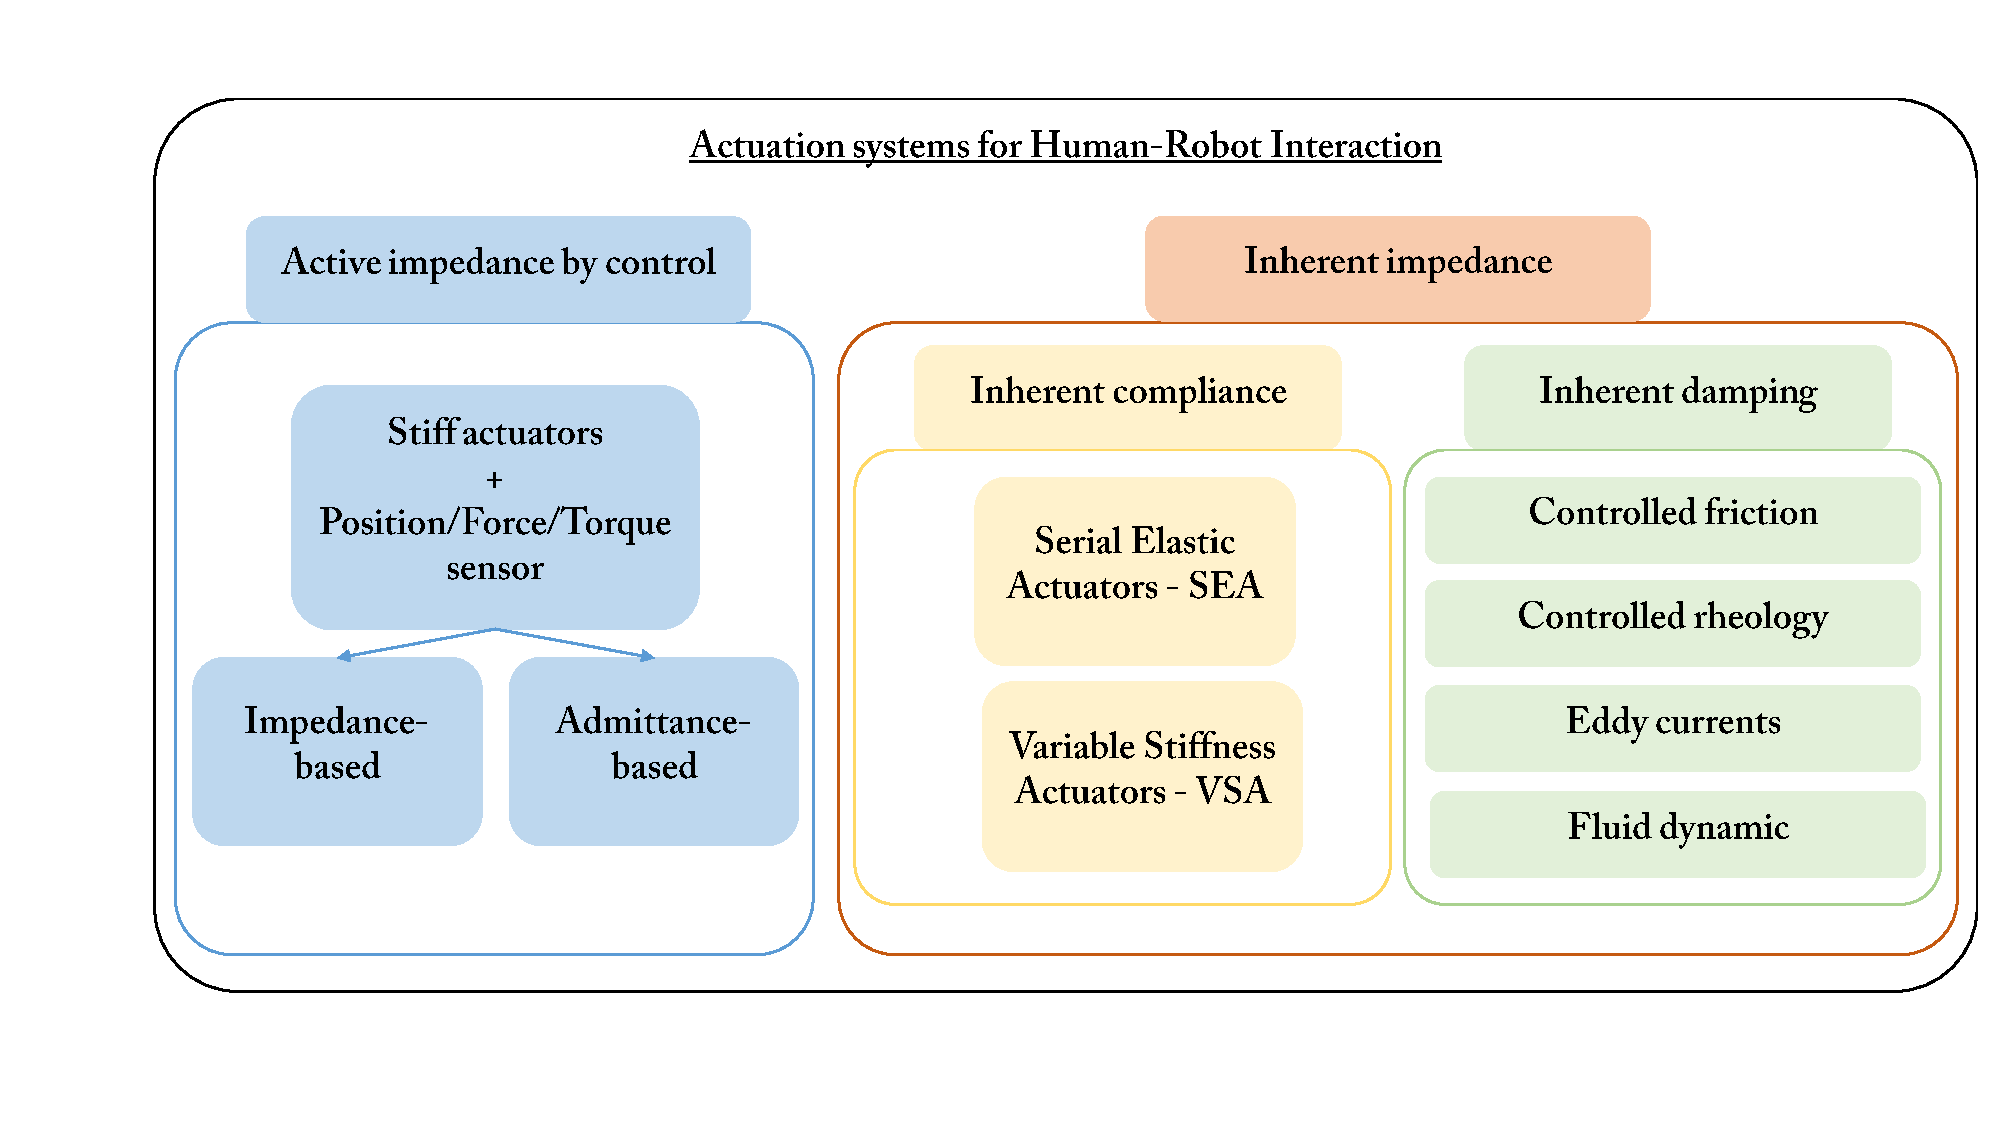
\includegraphics[width=1 \columnwidth]{actuators}
	\caption{Schema of variable impedance actuation systems for human-robot interaction. The impedance can be simulated and  actively changed by control (this relies on position and torque sensors) or can be an inherent mechanical property of the actuator. In the latter case the mechanical stiffness can be a fixed value (SEA) or can be adjusted (VSA), and the damping can be controlled.}
	\label{fig:exosActuators}
\end{figure}
%
\begin{figure}[htb]
	\centering
	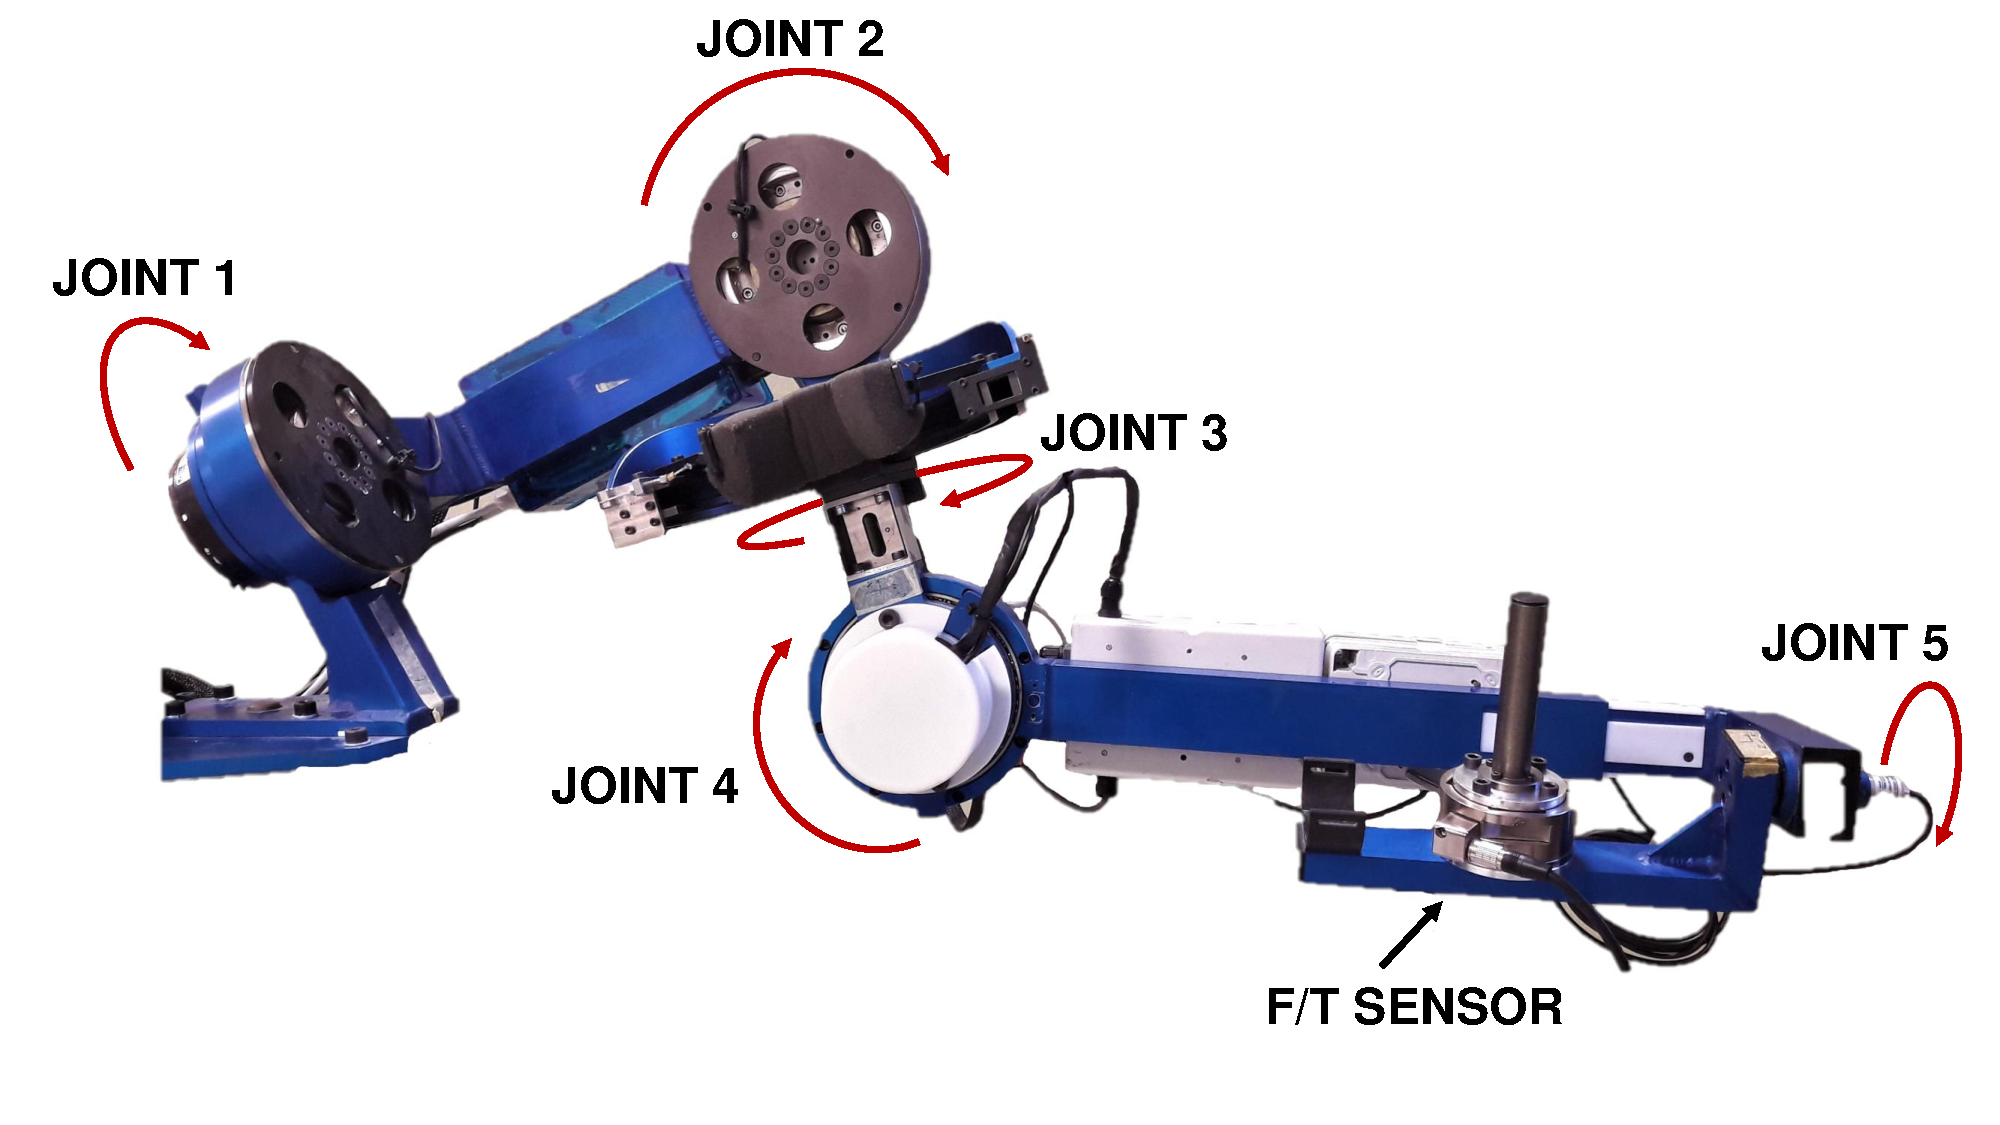
\includegraphics[width=0.95\columnwidth]{RehabDescription} 
	\caption{The Rehab-Exos. It is a 5 DOF upper-limb exoskeleton  with 4 actuated joints. The joints $J_1$, $J_2$ and $J_4$ share the same characteristics: high reduction ratio (100:1) by means of harmonic drive, embedded torque sensor and maximum actuation torque of 150 \ Nm. The joint $J_3$ is composed by a semi-circular guide actuated by a DC motor through tendon transmission. Joint $J_5$ is passive and the exoskeleton is equipped of a force/torque sensor at the end-effector that is used for evaluation purposes.}
	\label{fig:rehabexos1} 
\end{figure}
%
\par Solutions based on joint torque sensor have been proposed in the last years mostly for lower limb exoskeletons. In \cite{kim2015design} and in \cite{aguirre2011design} two knee exoskeletons based on joint torque sensor were presented; the latter exoskeleton implements an admittance control based on the torque sensor reads. In \cite{hwang2015method} the torque sensor for a lower limb exoskeleton allows to accurately estimate the human muscular torque that were exerted during the human-robot interaction. The advantage of joint torque sensor based solutions is their compactness and robustness, but when the torque sensor is embedded in the joint it is sensitive to the link inertia in addition to the human interaction torques, thus affecting the system transparency. A mechanical solution is presented in \cite{zanotto2013improving} where the transparency of a lower-limb exoskeleton has been improved by positioning the force/torque sensor on the supporting cuffs, that is at the interaction point between the human leg and the exoskeleton.
\par Even if SEA and VSA are less compact then traditional actuators, for example \cite{cestari2014ares} proposed a solution based on a VSA for an exoskeleton of the leg that reduced the lateral size and integrates a torque sensor based on spring's deflection reads. Sensors used to measure these deflections are generally encoders \cite{dos2017design} and potentiometers \cite{junior2016series}; the latter usually require custom mechanical supports to avoid errors related with its sensitivity to misalignments.
While the deflection based force estimation becomes a most widely utilized method for the SEAs and VSAs and performs fidelity force control performance in various robotic applications, there are still difficulties because of the practical issues such as spring deflection measurement error or noise of the encoder signal \cite{lee2018integrated}. These factors have much negative impact on SEA with high stiffness. In \cite{leal2018polymer}, for example, a polymer optical fiber has been mounted on the torsional spring of a SEA to read angles and torques in a more accurate way without considerably enlarging the size of the actuator at the cost of a more specific system electronics.
\par Thus, the use of inherent compliant actuation systems rather than achieving compliance by control systems is not a trivial choice and it depends on the desired mechanical features and is the result of a trade-off among compactness, weight, simplicity, costs, safety, efficiency and compliance.
A good trade-off that prefer compactness, simplicity and uses just one motor is an active impedance by control actuation system that integrates an elastic component to transmit and to measure axial torques at the same time.

\par In this paper we address the issue of a collaborative robot behavior, by designing an upper limb exoskeleton based on joint torque actuators endowing joint torque sensors and extend our previously work presented in \cite{solazzi2014interaction}. 
The Rehab-Exos allows to obtain a physical interaction characterized by good transparency and force rendering accuracy, it is capable to exert a wide range of forces and at the same time it exhibits high position accuracy due to high gear reduction ratio.
\par The first part of the paper widely treats the critical issue due to the use of a torque sensor embedded in the joint and in particular the sensitivity to non-axial load has been studied. Then, in the second part the joint model and the control technique are presented.
\par In particular, for what concern transparency we propose an interaction torque control that take into account the multi-dof non linear system dynamics and provide a compensation of non-linear effects such as inertial and gravity components, to achieve an accurate estimation of human interaction force.
This is accomplished by a single joint optimum observer that ensures joint torque tracking, while a centralized control estimates and compensates for the dynamics of the whole system. Moreover, we have evaluated the effect of dynamic compensation on system transparency highlighting good results.
\par To validate the proposed control as well as the chosen mechanical architecture, the full-state feedback control  has been compared with a basic feedback control and a passivity-based feedback control in two tasks: the zero desired force and the contact with a virtual stiff flat surface. 
For what concern haptic rendering, we evaluate at geometrical level the quantitative and qualitative behavior of the proposed controller and we compared it with the other two implemented controllers.
Results reward the chosen mechanical and control strategy as presented in the last part of this paper.
 
\par This paper is structured as follows: Section \ref{sec:systemDesign} presents the design of the Rehab-Exos with a particular focus on the strain gauge-based torque sensor design and issues. Section \ref{Single joint model} provides a mathematical model of the single joint whereas in the Section \ref{Full dynamics model} the full dynamics model of the Rehab-Exos is described. Section \ref{sec:Full_state_feedback_controllers} explains the proposed full state feedback controller and recalls two torque controls already known in literature. Section \ref{sec:experimentsResults} presents the experiments and the obtained results.
Finally, discussions and conclusions are addressed in Sections \ref{sec:discussion} and \ref{sec:conclusion} respectively.  

%
%Active exoskeleton systems are robotic devices that can be worn on the user's body, implying that they should satisfy requirements of safety and better compliance.
%After the Fukushima event in Japan, the application of these human-robot interfaces in the area of rescue robotics and teleoperation has became an emerging field of research,
%for which the development of upper limb active exoskeletons with dexterous manipulation abilities has become a hot topic of research.
%Another relevant sector of application of active exoskeletons is represented by neuro-motor rehabilitation post-stroke \cite{lo2012exoskeleton}, where different prototypes and commercial solutions have been recently proposed.
%
%
%While the general rationale for the design of high performance haptic interfaces are the satisfaction of the requirements of high force fidelity, transparency
%and backdrivability, specific issues need to be addressed in exoskeleton design in terms of safety, kinematics and ....
%
%For what concerns, upper limb exoskeletons, we should consider:
%\begin{description}
%\item[User requirements] Safety: the structure is always in close contact with the user
%\item[Design issues, kinematics, mechanical design]
%The kinematics should be adjusted to user arm, Possibility of adjusting the size of the system to avoid internal forces
%Complexity of shoulder motion, Non periodicity of upper limb movement compared to lower limb, Intrinsic 3D spatial motion Both left and right arm schemes should be implementable
%\item[Design issues, control] Low inertia should be achieved, possibility of employing force sensors, Remote vs. local actuation, High forces required (no gravity cancellation provided by support elements e.g., support plans)
%\end{description}
%
%%In SSSA there is a consolidated experience in the design and development of new exoskeleton systems \cite{frisoli2005new}, as shown in figure~\ref{fig:exos@SSSA}.
%
%%%%%%%%%%%%%%%%%%%%%%%%%%%%%%%%%%%%%%%%%%%%%%%%%%%%%%%%%%%%%%%%%%%%%%%%%%%%%%%%%%%%%%%%%%%%%%%%%%%%%%%%%%%%%%%%%%%%
%%%%%%%%%%%%%%%%%%%%%%%%%%%%%%%%%%%%%%%%%%%%%%%%%%%%%%%%%%%%%%%%%%%%%%%%%%%%%%%%%%%%%%%%%%%%%%%%%%%%%%%%%%%%%%%%%%%%
%%%%%%%%%%%%%%%%%%%%%%%%%%%%%%%%%%%%%%%%%%%%%%%%%%%%%%%%%%%%%%%%%%%%%%%%%%%%%%%%%%%%%%%%%%%%%%%%%%%%%%%%%%%%%%%%%%%%
%%%%%%%%%%%%%%%%%%%%%%%%%%%%%%%%%%%%%%%%%%%%%%%%%%%%%%%%%%%%%%%%%%%%%%%%%%%%%%%%%%%%%%%%%%%%%%%%%%%%%%%%%%%%%%%%%%%%

%DIFDELCMD < 
\section{System design} \label{sec:systemDesign}
%\hldone{Done}
The Rehab-Exos is an active robotic exoskeleton (\figurename \ \ref{fig:rehabexos1}) which is designed with the idea to be compact, easily reconfigurable and to have a good trade-off between transparency and force replication.
It was conceived for rehabilitation applications and it is designed in such a way to generate controlled contact forces/torques not only at its end-link handle, but also at  intermediate links. When the user is wearing the device he can control the full force interaction with the exoskeleton and guide/be guided involving all articulations of the arm (wrist, shoulder, elbow). 
The physical interaction between user and exoskeleton is monitored by the joint torque sensors which performances depend on several design and implementation aspects that are addressed in subsection \ref{subsec:DesignTorqueSensor}.
%%%%%%%%%%%%%%%%%%%%%%%%%%%%%%%%%%%%%%%%%%%%%%%%%%%%%%%%%%%%%%%%%%%%%%%%%%%%%%%%%%%%%%%%%%%%%%%%%%%%%%%%%%%%%%%%%%%%
%%%%%%%%%%%%%%%%%%%%%%%%%%%%%%%%%%%%%%%%%%%%%%%%%%%%%%%%%%%%%%%%%%%%%%%%%%%%%%%%%%%%%%%%%%%%%%%%%%%%%%%%%%%%%%%%%%%%
\subsection{Mechanical design of the Rehab-Exos} 
%\hldone{Done}
\label{subsec:mechanicalDesign}
As depicted in \figurename \ \ref{fig:rehabexos1} and in \figurename \ \ref{fig:rehabexosSchema}, the exoskeleton has a serial architecture isomorphic with the human kinematics that comprises: a shoulder joint  fixed in space and composed by three active joints $J_1$, $J_2$ and $J_3$; an active elbow joint $J_4$; and a passive revolute joint $J_5$ allowing for wrist prono/supination.  For a more detailed description of both Rehab-Exos and actuation groups, the reader can refer to \cite{vertechy2009development}.
%\begin{figure}[htb]
%	\centering
%	\subfigure[Exoskeleton kinematics]{\includegraphics[width=0.49\columnwidth]{\figpath{exos1}}\label{fig:exos_kinematics}}
%	\subfigure[CAD section of the joint actuator ]{\includegraphics[width=0.49\columnwidth]{\figpath{JointActuator}}\label{fig:exos_actuator}}
%	\caption{The Rehab-Exos CAD model showing overall kinematics and actuator structure}
%\end{figure}
\begin{figure}[]
	\centering
	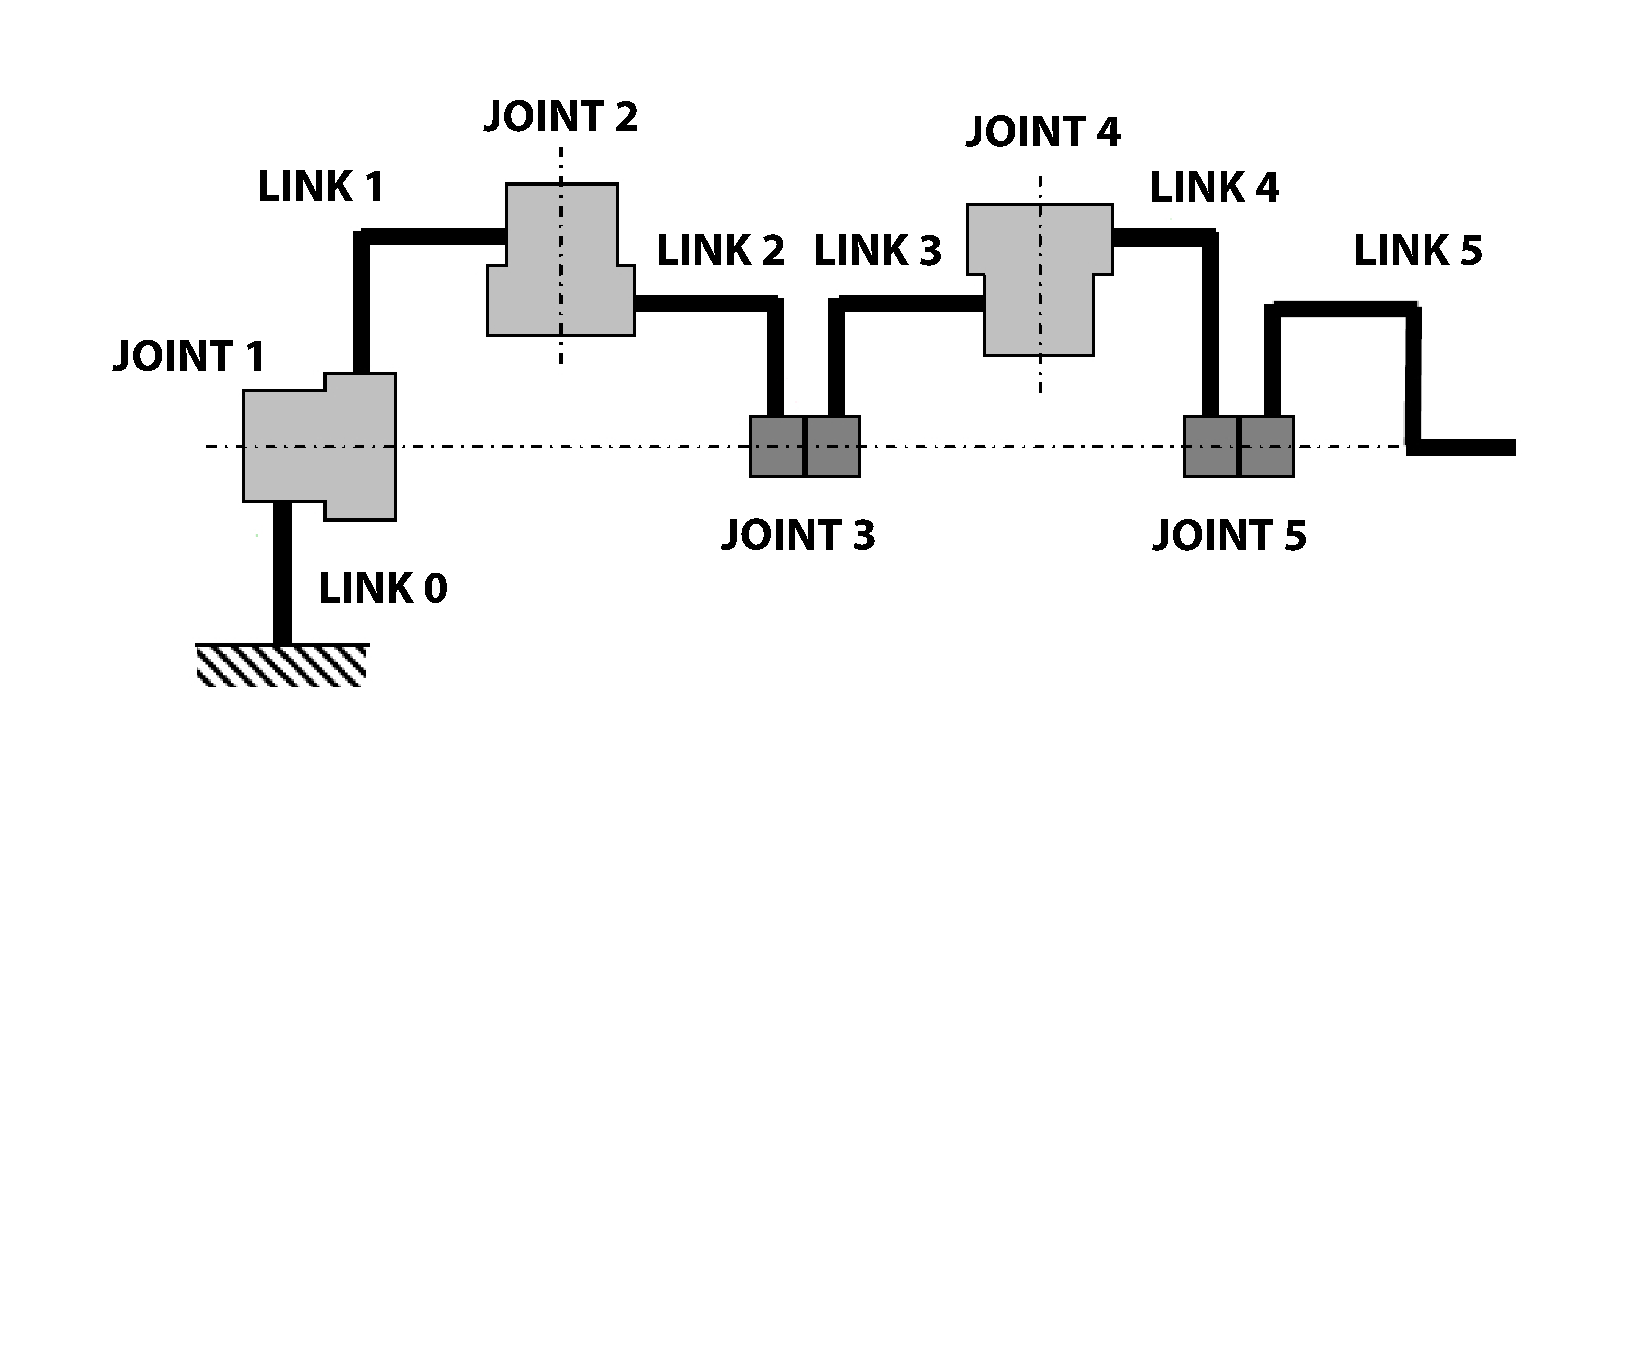
\includegraphics[width=0.9\columnwidth]{SchemaExos}
	\caption{A schematic representation of the Rehab-Exos exoskeleton.}
	\label{fig:rehabexosSchema}
\end{figure}
%
%
\begin{figure}[]
	\centering
	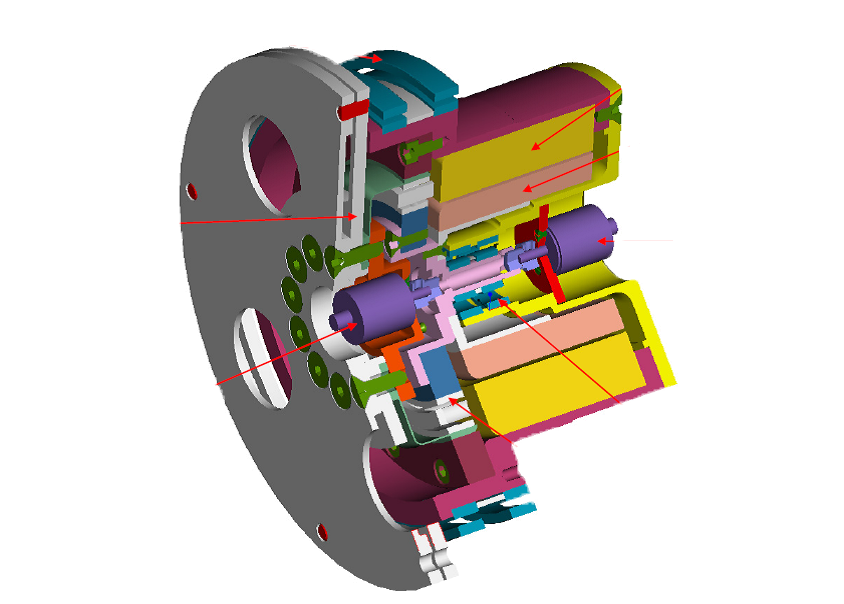
\includegraphics[width=0.7\columnwidth]{JointActuator}
	\caption{CAD section of the $J_1$, $J_2$ and $J_4$ joint actuator of the Rehab-Exos.}
	\label{fig:exosActuatorCAD}
\end{figure}
%
\par The three joints $J_1$, $J_2$ and $J_4$ of the exoskeleton are motorized through identical actuation groups. Each joint features a custom-made frame-less brush-less torque motor integrating a compact Harmonic Drive (HD) component set. The actuator provides a joint output torque equal to $150\ Nm$ with an overall weight equal to $3.7\ Kg$ and a motor shaft inertia reduced to the joint output shaft $Jm = 3.7\ Kgm^2$. The Harmonic Drive performs a reduction equal to 100:1. Due to the adopted mechanical components, the joints feature limited back-drivability at motor power-off and limited mechanical complexity to ease maintenance as well as reduce costs. A CAD section of the $J_1$, $J_2$ and $J_4$ joints is depicted in \figurename \ \ref{fig:exosActuatorCAD}.
Joint $J_3$ is characterized by a tendon transmission that is used to transmit the actuation torque through an open semi-circular guide. More detail on the joint $J_3$ can be found in \cite{vertechy2009development}.

\subsection{Design aspects of the strain gauge based torque sensor}
%\hldone{Done}
\label{subsec:DesignTorqueSensor}
The three joints $J_1$, $J_2$ and $J_4$ have a torque sensor featuring a four-spoke-shape geometry. 
Despite further augmenting the actuation group compliance, the availability of joint-torque sensors enables for multi-contact force control at multiple points distributed over the links and, additionally, makes it possible: 1) to close a stable high-bandwidth torque inner loop around each joint which is weakly affected by robot link variable inertia; 2) to suppress robot vibrations produced by the inherent transmission compliance (Harmonic Drive); 3) to reduce internal disturbance torques caused by actuator and reducer (for instance friction losses, actuator's torque ripples and gear teeth wedging actions); to measure externally applied forces/moments and complex non-linear dynamic interactions between joints and links.
\par The sensor consists of two fully balanced strain gauge bridges placed on different beams of the spoke, which is located at the joint output shaft. 
%
%
\begin{table}[t]
	\renewcommand{\arraystretch}{1.3}
	\caption{Characteristic dimensions of the torque sensor}
	\label{tab:sensorDimension}
	\centering
	\begin{tabular}{c c}
		\hline \hline
		\bfseries Dimension & \bfseries Value [$mm$] \\
		\hline
		R & 78 \\
		r & 38 \\
		L & 24 \\
		a & 4 \\
		round radius & 2 \\
		\hline \hline
	\end{tabular}
\end{table} 
%
\begin{figure}[]
	\centering
	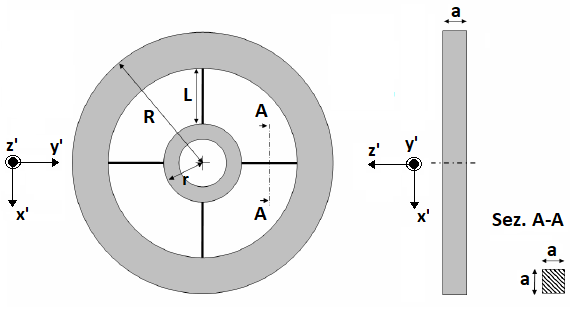
\includegraphics[width=0.7\columnwidth]{sensorDimensions}
	\caption{Characteristic dimensions of the torque sensor.}
	\label{fig:sensorDimensions}
\end{figure}
%
The sensor is made by AISI 630 steel, an harmonic steel exhibiting yield strength of 1950 MPa, Young's modulus of 196 GPa and has been dimensioned to exhibit low weight and high sensitivity to axial moments.
The axial torsional stiffness of the sensor is $k_s = 30 \ kNm/rad$ and can be calculated as in \eqref{eqn:sensorStiffness}.
\begin{equation}
\label{eqn:sensorStiffness}
k_{s} = \frac{\tau}{\theta} = \frac{Ea^4(r+L(1-Q))}{3L^2(1/2-Q)}	
\end{equation}
where the adimensional parameter Q is given by
\begin{equation}
\label{eqn:adimensionalQ}
Q = \frac{3r+L}{6r+3L}	
\end{equation}
where, according to \figurename \ \ref{fig:sensorDimensions}, $R$ is the radius of the external sensor ring, $r$ is the radius of the internal sensor ring, $L$ is length of the beams and $a$ is the side length of the beam section.
The characteristic dimensions of the sensor are reported in \tablename \ \ref{tab:sensorDimension}.
Moreover, the overall joint torsional stiffness reduced to the joint output shaft is $k = 11.38\ kNm/rad$.
\par The position of the strain gauges on the beam is a trade-off: if they were positioned in the middle of the beam the sensor sensitivity would be low, on the contrary, if they were positioned near the extremities the sensor reads would be affected by the non-linearities of the rounds of the beam. The selected distance from the extremities was $p = 1/8 \ L = 3 \ mm$.
To estimate the strain of the beam in a given point with distance $p$ from the inner ring under a certain axial torque $\tau$, the normal tension $\sigma_p$ that acts on that point $p$ needs to be computed as
\begin{equation}
\label{eqn:normalTensionOnBeam}
\sigma_p = \frac{3\tau((1-Q)L-p)}{2a^3((1-Q)L+r)}	
\end{equation}
and then the strain follow as 
\begin{equation}
\label{eq:strainEq}
\epsilon_A= \frac{\sigma}{E}
\end{equation} 
where $E$ is the Young's modulus.
\par Theoretically, i.e. using \eqref{eq:strainEq}, at $3 \ mm$ from the inner ring and under an axial torque of $120 Nm$,  a maximum strain of $2.7*10^-3 \ m$ is obtained.
The same test has been conducted using a FEM software tool (Ansys\textregistered) because the surface of the strain gauge is not negligible compared to the beam one (see \figurename \ \ref{fig:strainGaugeDeformation}) obtaining a maximum strain of $1.98*10^-3 \ m$.
The strain of each strain gauge when a $1 \ Nm$ load is applied can be shown in \tablename \ \ref{tab:sensorStrain}.
\begin{table}[]
	\renewcommand{\arraystretch}{1.3}
	\caption{Strain of the 4 strain gauges}
	\label{tab:sensorStrain}
	\centering
	\begin{tabular}{c c c c}
		\hline \hline
		\bfseries Probe 1 [m] & \bfseries Probe 2 [m] & \bfseries Probe 3 [m] & \bfseries Probe 4 [m]\\
		\hline
		1.65e-5  & -1.33e-5 & -1.91e-5 & 2.2546e-5\\
		\hline \hline
	\end{tabular}
\end{table} 
%
\par An important characteristic of the torque sensor is the sensitivity to non-axial moments, thus an experimental test has been conducted to compute the sensitivity, i.e. a predetermined non-axial torque has been exerted on the sensor in 4 configurations (angle) of the sensor.
Experimental results are reported in \tablename \ \ref{tab:sensorNonAxialResults} and the sensitivity is equal to
\begin{equation}
S_S=\frac{C_{mis}}{C_S}=0.067
\label{eq:sensitivityToNonAxLoad}
\end{equation} 
%
\begin{table}[]
	\renewcommand{\arraystretch}{1.3}
	\caption{Sensor reads to non-axial moments}
	\label{tab:sensorNonAxialResults}
	\centering
	\begin{tabular}{cc}
		\hline \hline
		\bfseries Applied Torque [Nm] & \bfseries Sensor reads per angle [Nm]\\
		$\;$ &	\begin{tabular}{cccc} $0^\circ$   & $45^\circ$ & $90^\circ$ & $180^\circ$ \end{tabular} \\
		\hline
		32 & \begin{tabular}{cccc} 1.6 & 2.4 & 2.2 & 2.3 \end{tabular} \\
		64 & \begin{tabular}{cccc} 2.9 & 4.8 & 4.4 & 4.4 \end{tabular} \\
		96 & \begin{tabular}{cccc} 4.5 & 7.5 & 6.9 & 6.9 \end{tabular} \\
		\hline \hline
	\end{tabular}
\end{table} 
The sensitivity to non-axial moments is relatively high compared to one mentioned in \cite{kashiri2017sensor}. %This non-ideal and non-linear characteristic were not found in the initial test-rig, instead non-axial loads are there in the multi-link mounted exoskeleton. 
%Despite the presence of the ball bearings, two factors influence the sensor readings. The first factor is the way the mechanical parts are assembled (assembly errors), the second is the non-axial loads influence on the sensor readings. 
\par The reason of these results has been investigated and two causes (or a combination of them) have been proposed. The first cause of error could be a strain gauges mounting misalignment. The second cause could be an excessive deformation of the sensor due to the non-axial moments. 
About the first hypothesis, the sensitivity of the strain gauges to non-axial load $C_S$ (when a flexible model of the HD is considered) due to strain gauges misalignment can be modeled as
\begin{equation}
S_{misal}= k_s \cdot (k_{ex} \cdot e_x + k_{e\theta} \cdot e_{\theta})
\label{eq:sensitivityMisalignment}
\end{equation}
where $k_s$ is a scaling factor equal to $7.87e^{-3}$, $k_{ex}$ is the sensitivity to linear mounting misalignment  equal to $3$, $k_{e\theta}$ is the sensitivity to angular mounting misalignment equal to $2.3$, whereas $e_x$ and $e_{\theta}$ are the positional and angular misalignment errors respectively (see \figurename \ \ref{fig:strainGaugeMisalignment}). Equation \eqref{eq:sensitivityMisalignment} and the measured sensitivity of 0.067 lead to a misalignment errors of millimeters and decades of degree, but these values are over the actual misalignment the installation operator may have introduced as can be seen in \figurename \ \ref{fig:strainGaugeParticular}.
%
\begin{figure}[]
	\centering
	\subfigure[]{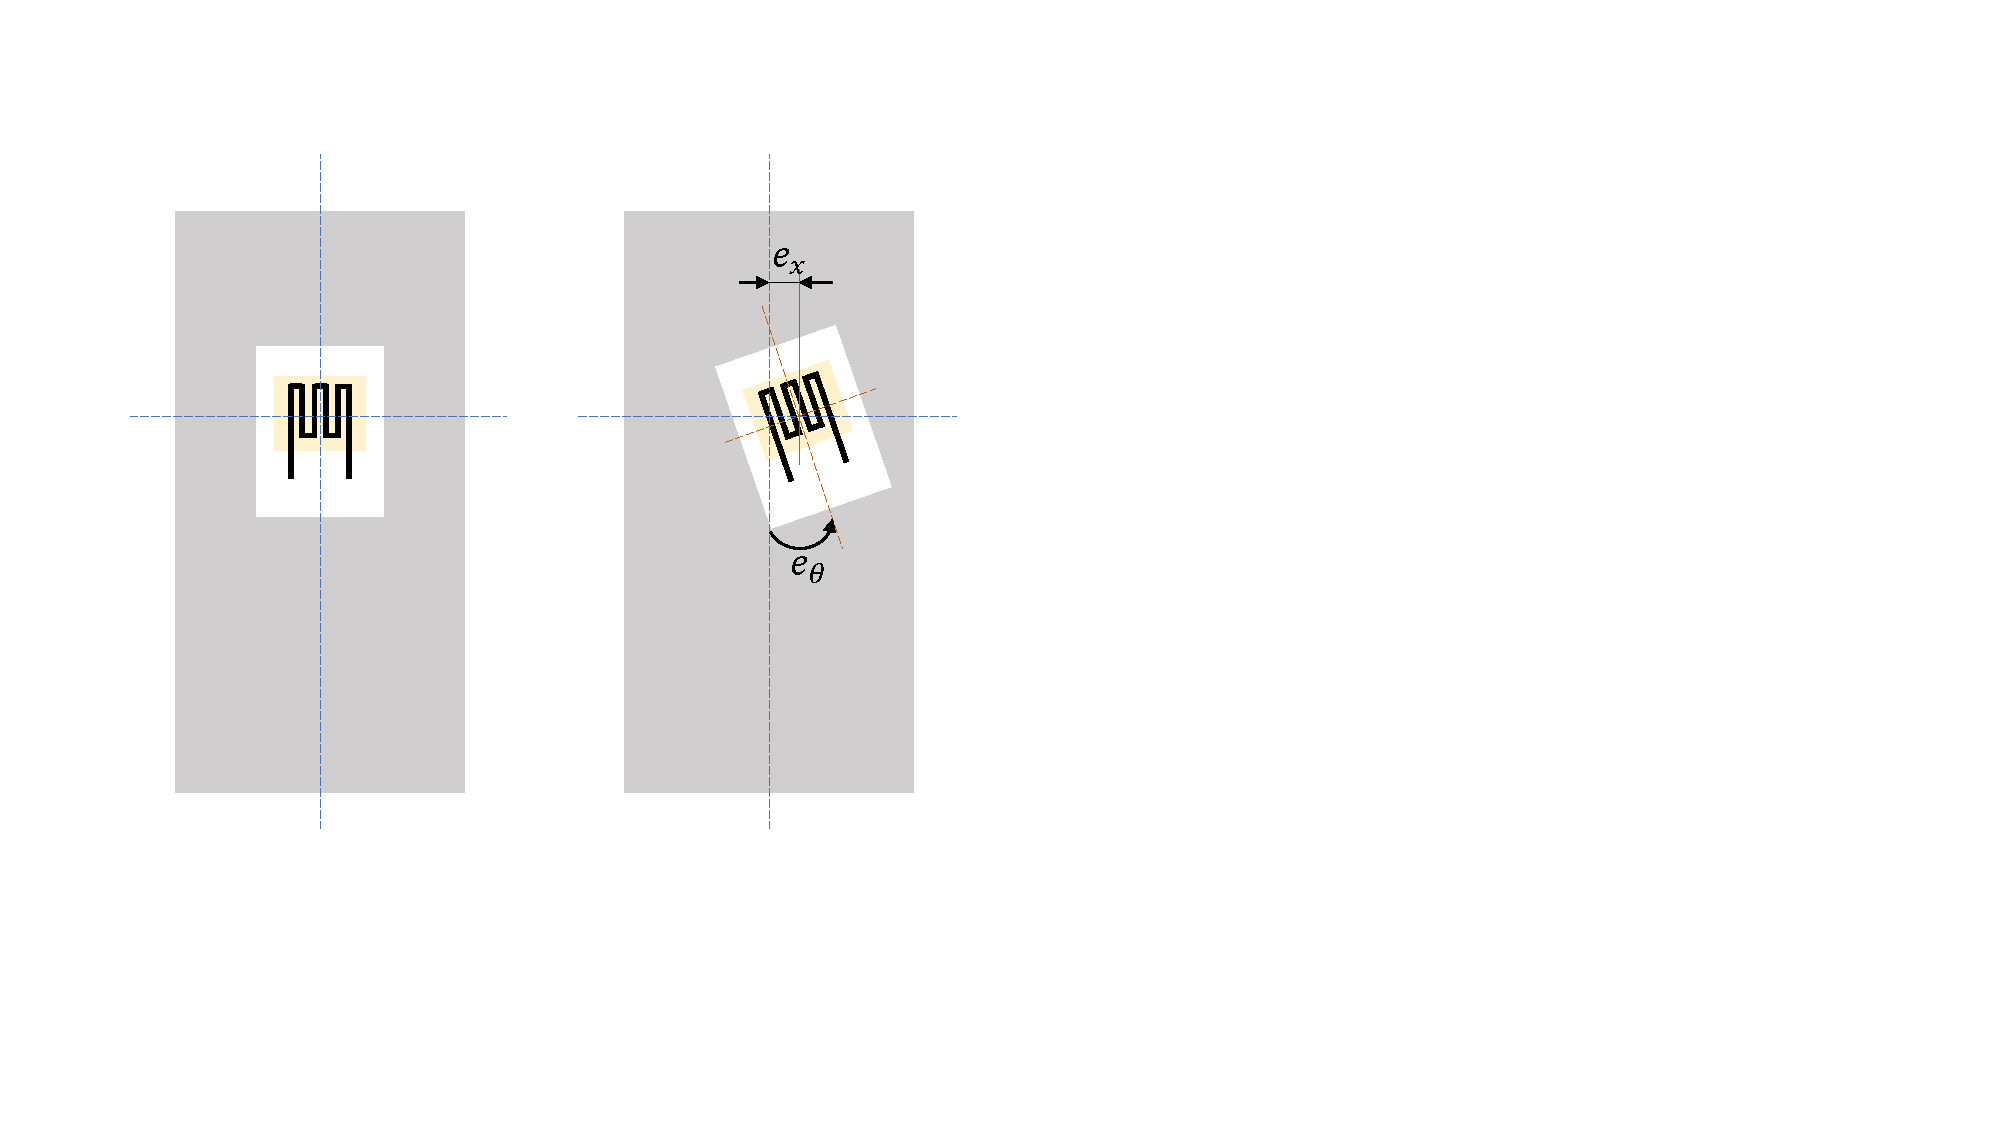
\includegraphics[height=0.35\columnwidth]{erroreMontaggioSensore} \label{fig:strainGaugeMisalignment}}
	\subfigure[]{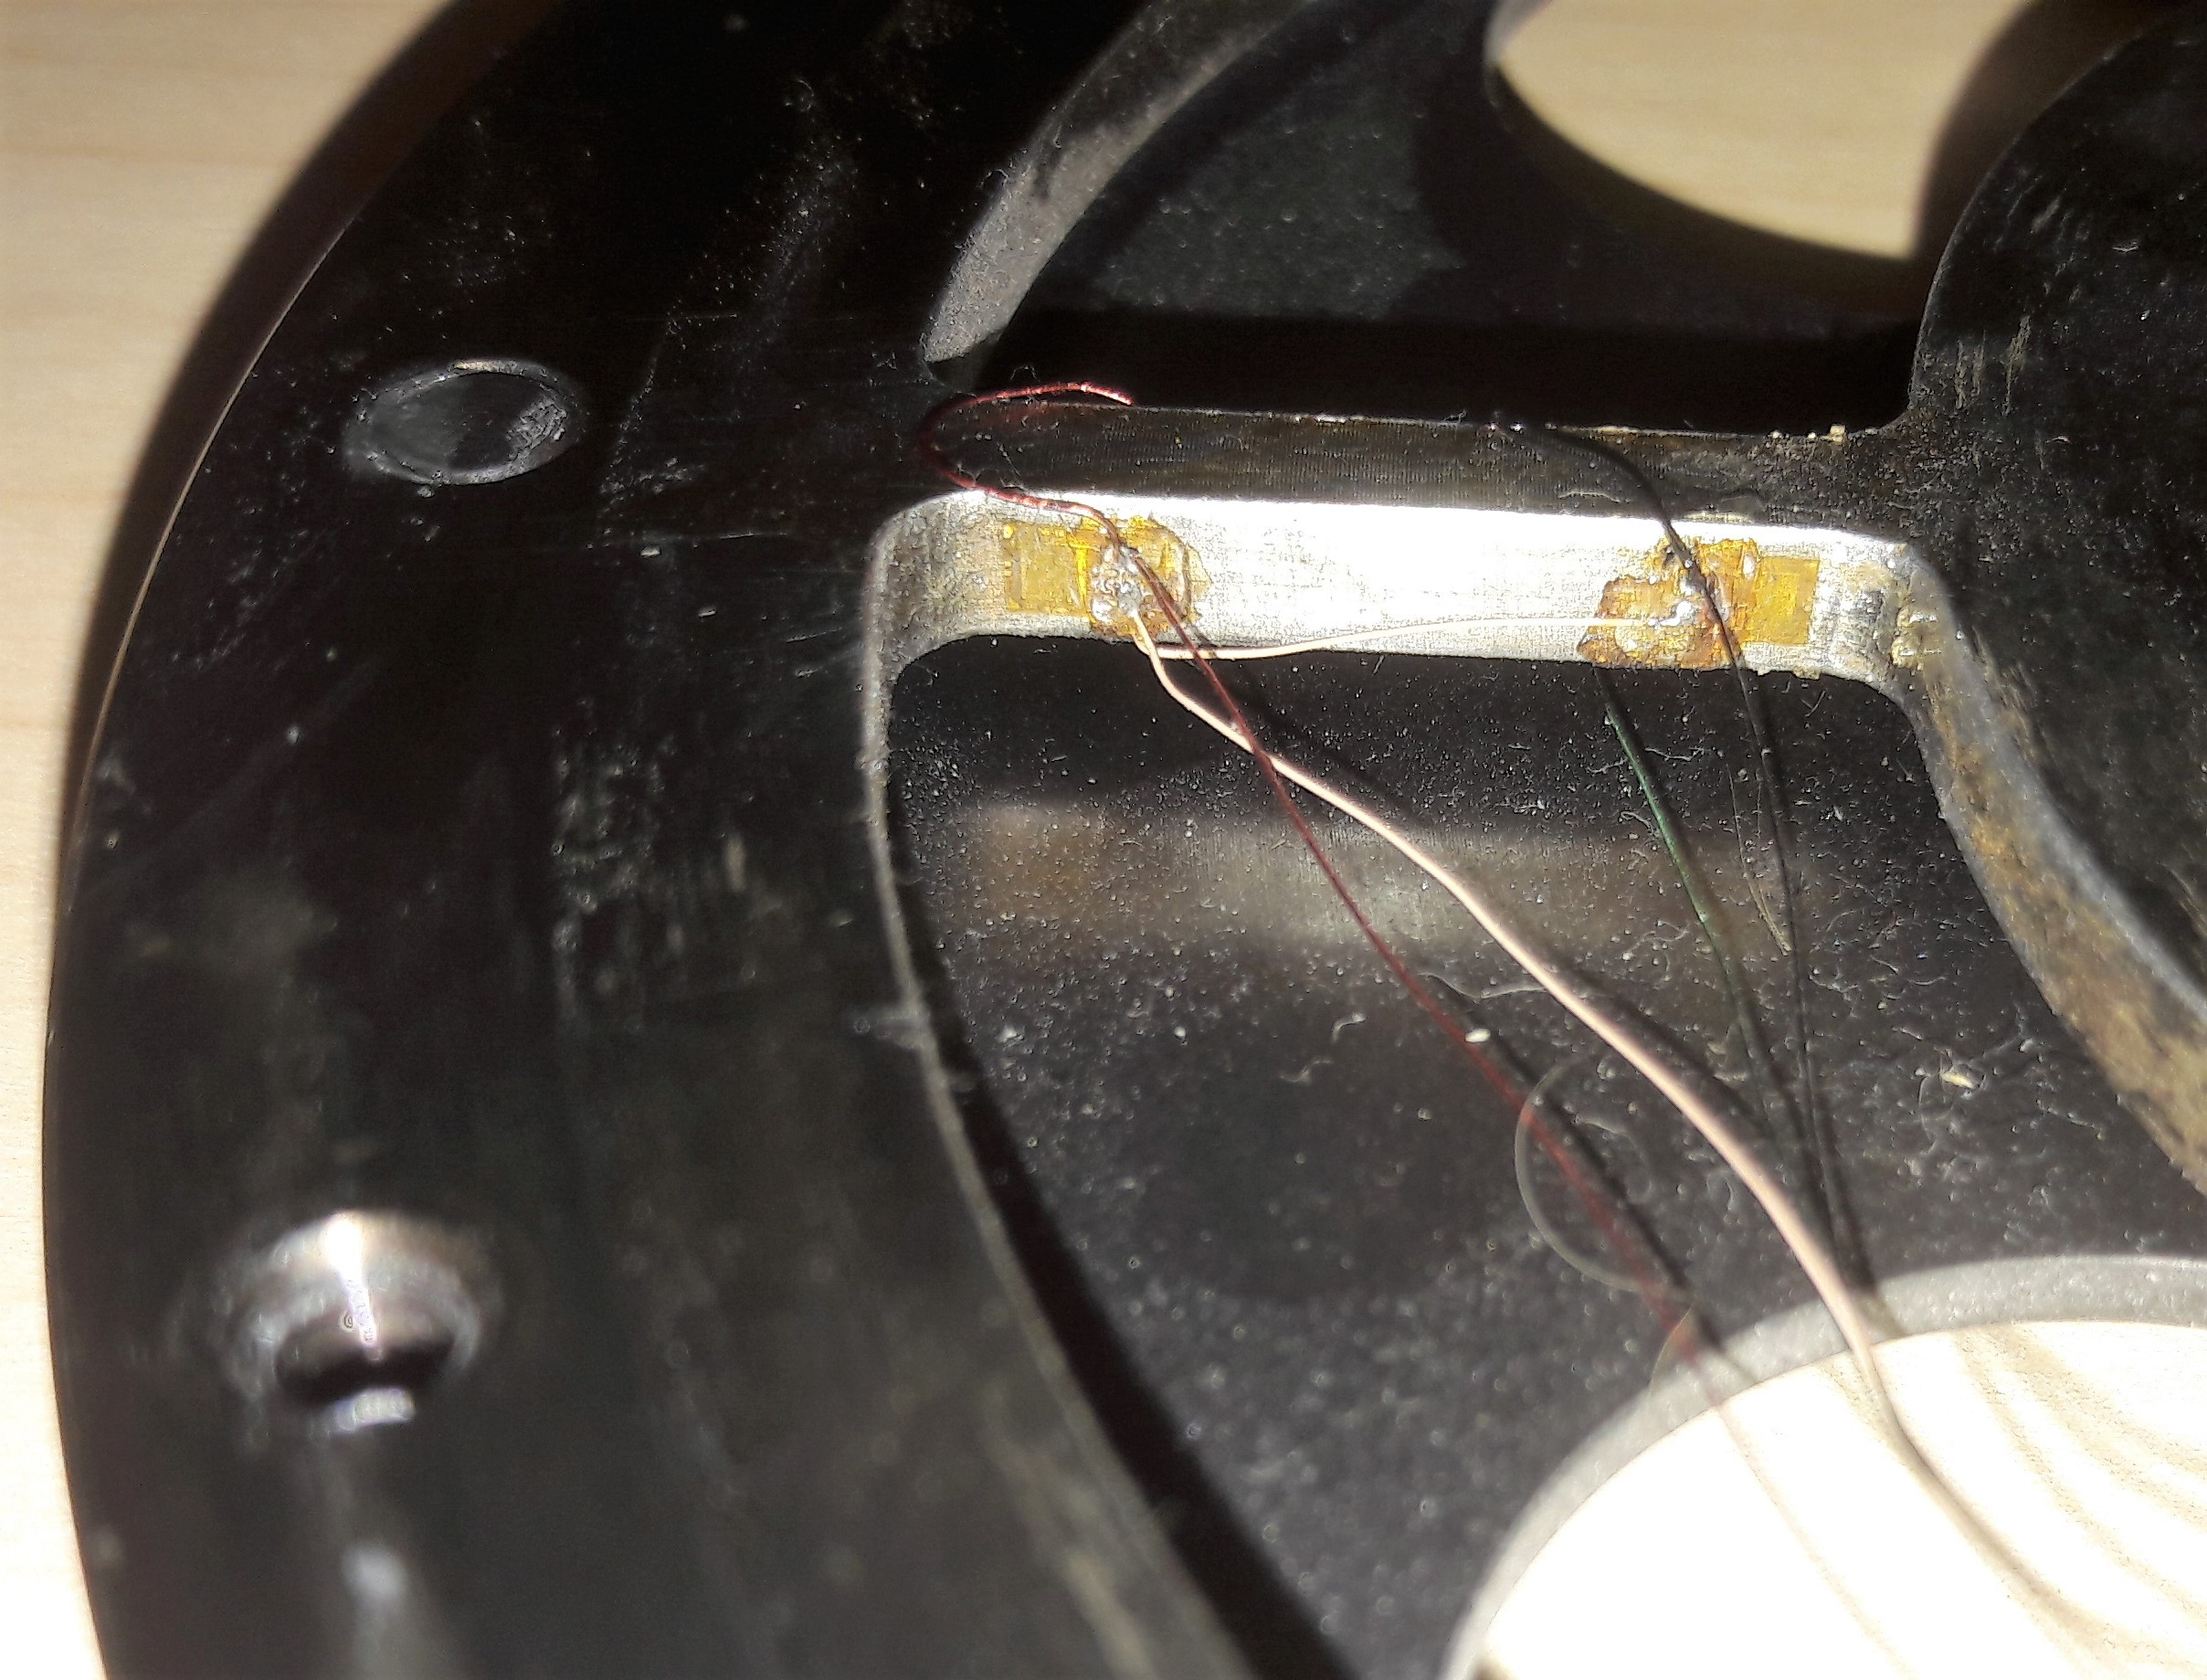
\includegraphics[height=0.32\columnwidth]{strainGaugeParticular.jpg} \label{fig:strainGaugeParticular}}
	\caption{A possible cause of high sensitivity to non-axial load is the strain gauges's mounting misalignment. The linear displacement $e_x$ and the angular one $e_{\theta}$ are highlighted in (a). A detail of the mounted strain gauges on the torque sensor in (b).} 
\end{figure}

About the second hypothesis it is worth to notice that the sensor from a structural point of view is in series to the HD and this series is in parallel with a couple of bearings. This parallel chain composes a hyper-static system (see \figurename \ \ref{fig:schemaGiuntoEMolle}), therefore the excessive sensitivity may be due mounting misalignment of the mechanical parts of the chain. 
%
\begin{figure}[]
	\centering
	\subfigure[]{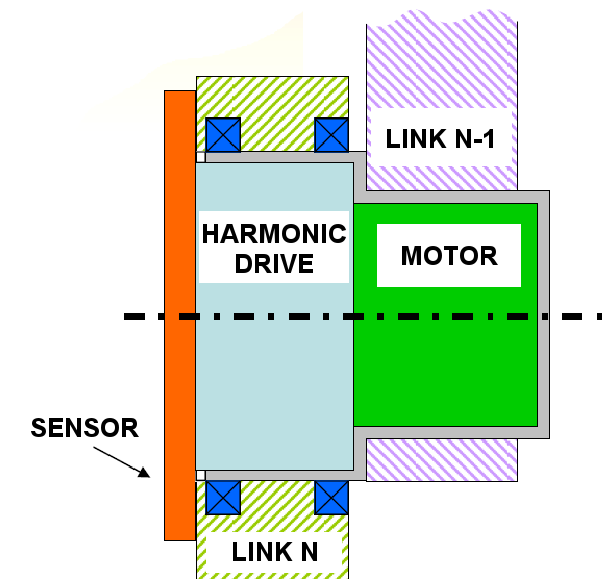
\includegraphics[width=0.49\columnwidth]{schemaGiuntoMod}\label{fig:schemaLinkGiuntoSens}}
	\subfigure[]{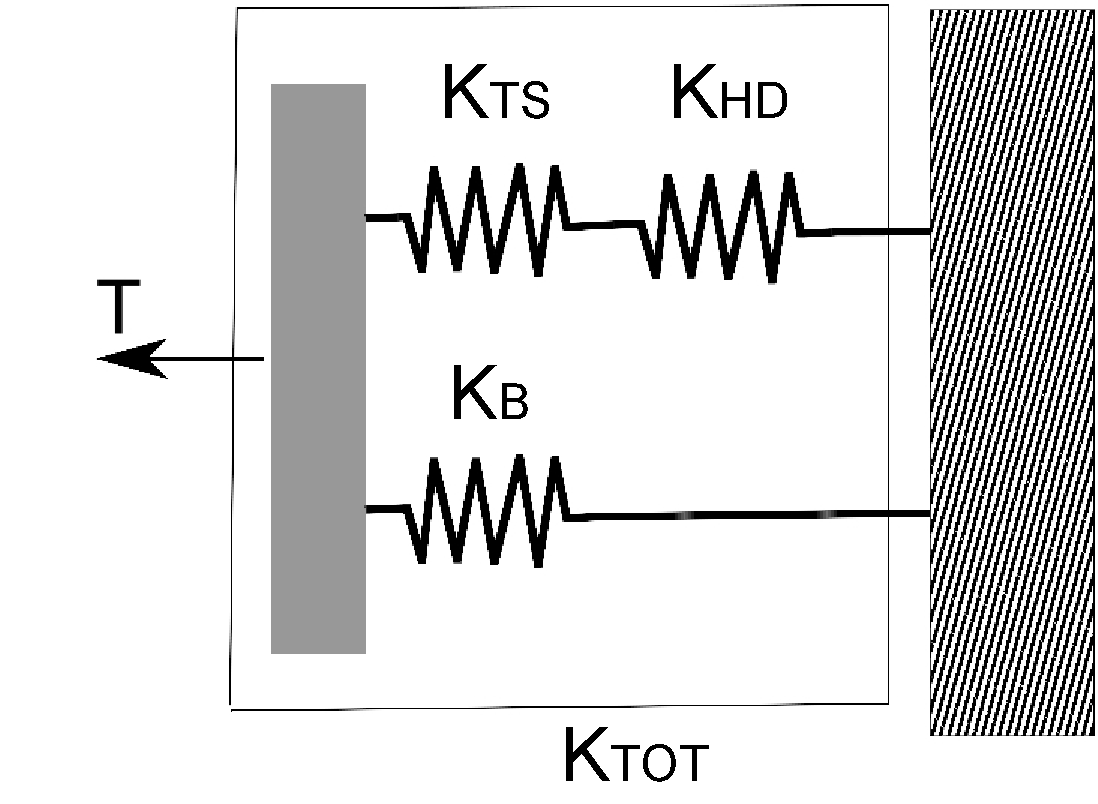
\includegraphics[width=0.49\columnwidth]{schemaMolle.pdf}\label{fig:schemaMolle}}
	\caption{In a), the schematic representation of the joint. The torque sensor is a series elastic element between the motor and the link n. The torque sensor is not structural and has been designed to transmit only axial torque. In b), the kinematic chain of the joint to non-axial loads. $K_{TS}$ and $K_{HD}$ are the stiffness of the torque sensor and of the Harmonic Drive to non-axial load respectively, whereas $K_B$ is the bearing stiffness.}
	\label{fig:schemaGiuntoEMolle}
\end{figure}
%
\par For the study of the hyper-static system a linear  elastic behavior of the system parts were supposed and the system response at non-axial moments was modeled as a mono-dimensional model as in \figurename \ref{fig:schemaMolle}.
The overall joint stiffness to non-axial moments $K_{TOT}$ was experimentally evaluated, whereas the non-axial moment stiffness of the torque sensor $K_{TS}$ and of the HD $K_{HD}$ were computed via FEM analysis. The FEM results are depicted in \figurename \ \ref{fig:strainGaugeDeformation} and the stiffness values are reported in table \tablename \ \ref{tab:nonAxialStiffness}.
%
\begin{figure}[]
	\centering
	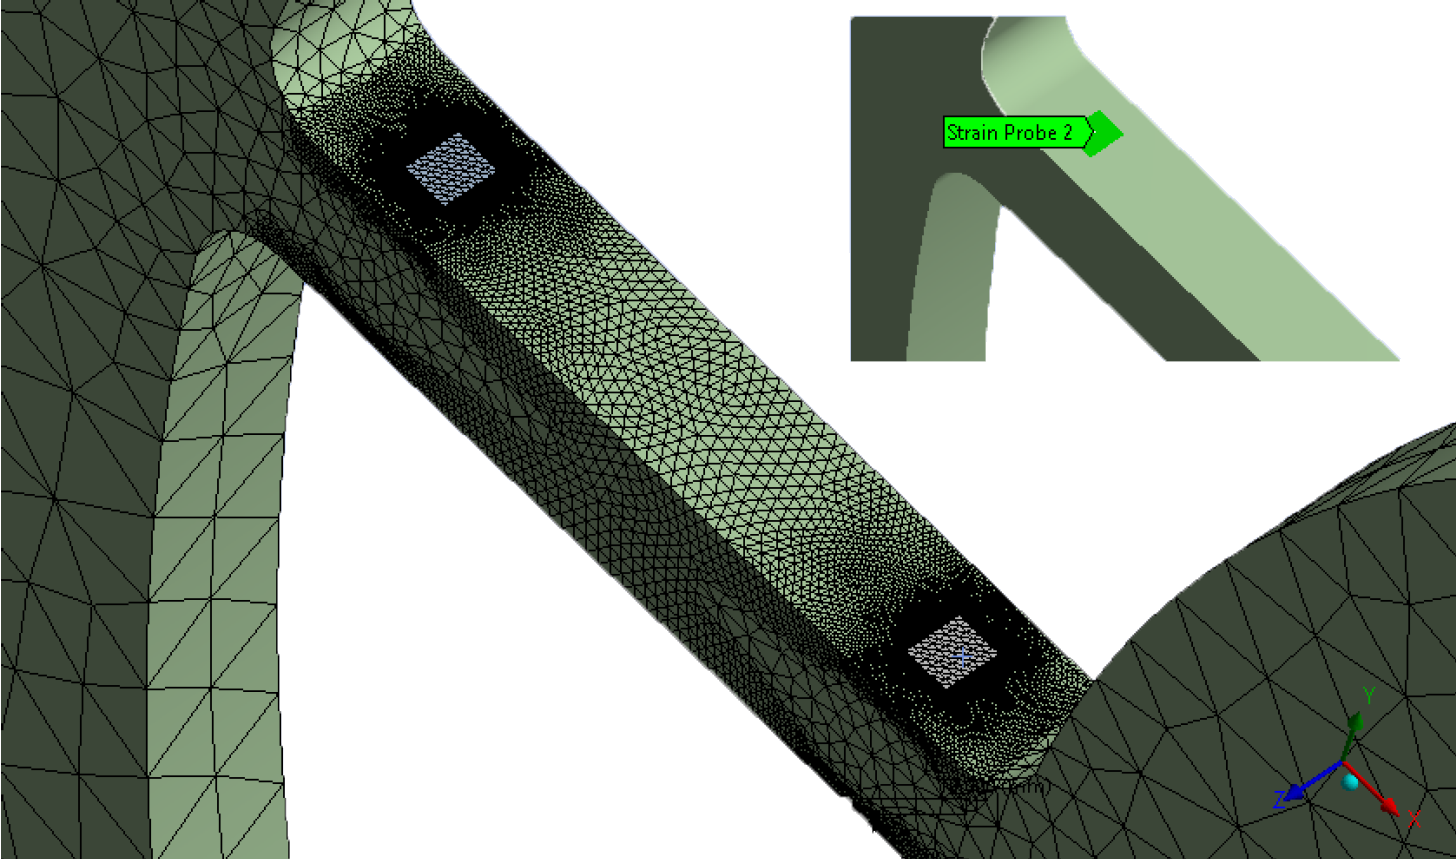
\includegraphics[width=0.7\columnwidth]{strainGaugeDeformation} 
	\caption{For the FEM analysis a more dense grid mesh for the zone of interest has been used. For each area the average strain along the radial direction has been computed.}
	\label{fig:strainGaugeDeformation}
\end{figure}
%
\begin{table}[]
	\renewcommand{\arraystretch}{1.3}
	\caption{Stiffness of the components}
	\label{tab:nonAxialStiffness}
	\centering
	\begin{tabular}{c c}
		\hline \hline
		\bfseries Component & \bfseries Stiffness [kNm/rad]\\
		\hline
		$K_{TS}$  & 4.1\\
		$K_{HD}$  & 0.4\\
		$K_{B}$   & 23.6\\
		\hline
		$K_{TOT}$   & 24\\
		\hline \hline
	\end{tabular}
\end{table}
%
%
\par A possible mounting misalignment of the hyper-static chain may be a collinear and/or concentric mounting misalignment between the sensor axis and the bearing axis. In this case, the HD works as an universal joint that connect the sensor (that is connected to the (n+1)-th link ) and the n-th link. The sensitivity to non-axial moments defined in equation \eqref{eq:sensitivityToNonAxLoad} and  the mechanical properties  in \tablename \ \ref{tab:nonAxialStiffness} lead to a theoretical mounting misalignment of about $0.5 \ mm$, but this value is not in agreement with the design tolerances and components data-sheets from which a misalignment of about $0.05 \ mm$ results in the worst case.
%
%The internal joint-torque sensor introduces controlled torsional compliance that is used at the same time to transmit joint torque actuation  from the motor to the link and to measure it. 
%The torque sensor is not structural and the mechanical transmission is parallel (see the scheme in \figurename \ \ref{fig:schemaLinkGiuntoSens}). The planar sprocket hub has been designed to be sensitive only to the torque along the motor axes exchanged between the motor on the link $n-1$ and the link $n$, while theoretically the torques along the other two axes are transmitted directly through the ball bearings between the link $n-1$ and the link $n$.
\par To summarize, unwanted sensor reads to non-axial load may be due to the combination of effects from sensor mounting misalignments and HD excessive deformation. 
\par In order to minimize this undesired effect the authors propose a method based on artificial neural networks (ANN) to characterize and compensate this non-linear behavior that results difficult to model.
%
%
Considering the ideal and linear sensor, the torque readings can be expressed as $\tau_s = k_v * v$, where $v$ is the measured voltage tension and $k_v$ is the torque sensor's voltage constant. In the real case it be can written $\hat{\tau}_s = k_v * v + \delta\tau$, where $\delta\tau$ is the non-linear influence on the sensor readings due to the mounting and non-axial loads.
By experimental evidence, it's possible to assert that the term $\delta\tau$ varies in a non-linear way with respect the exoskeleton pose (joint angles) and load.
\par The mounting errors influence the torque readings non-linearly with respect to the joint angle, while the non-axial torques depends in part on the interaction with human and in part on the dynamics and gravitational torques acting on the considered joint.
%\begin{figure}[htb]
%	\centering
%	\includegraphics[width=0.55\columnwidth]{\figpath{schemaGiuntoMod}}	
%	\caption{}
%	\label{fig:schemaLinkGiuntoSens}
%\end{figure}
%
\begin{figure}[]
	\centering
	\subfigure[]{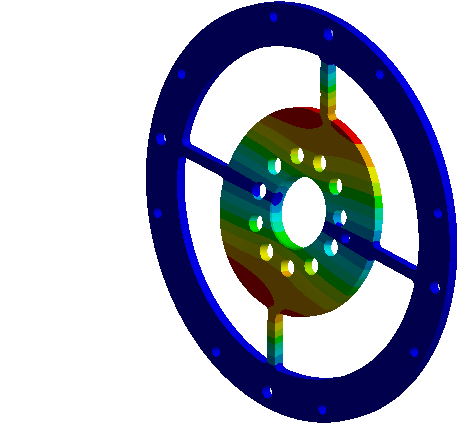
\includegraphics[height=0.4\columnwidth]{sensoreCarichiSpuri} \label{fig:sensoreCarichiSpuri}	}
	\subfigure[]{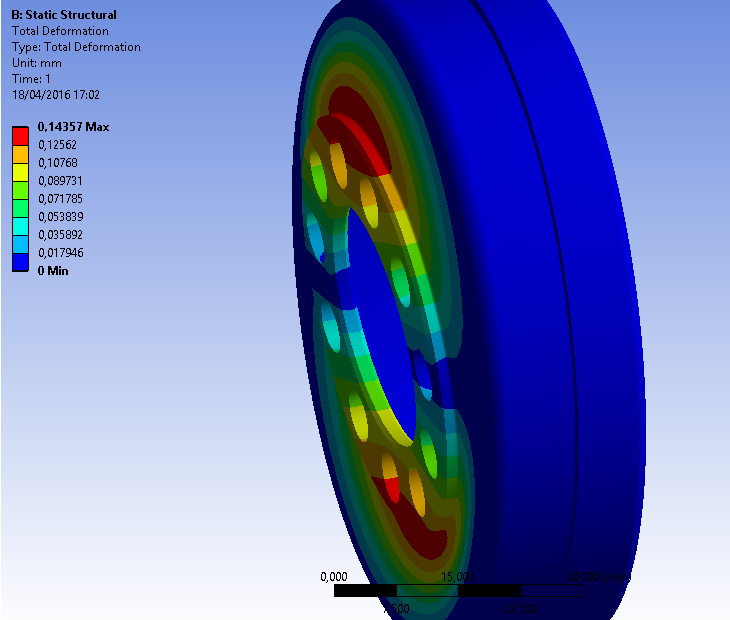
\includegraphics[height=0.4\columnwidth]{HDCarichiSpuri} \label{fig:HDCarichiSpuri} }
	\caption{The FEM analysis results of the torque sensor (a) and of the flexible spline (b) deformation under non-axial load.}
\end{figure}
%
%
For all the three sensors the $k_v$ constants have been experimentally evaluated. In order to minimize the effect of non-linear undesired term $\delta\tau$,  an ANN has been used. ANN is a mathematical approximation approach that is capable to infer non-linear behavior from experimental acquisitions. The ANN with 7 neurons in the hidden layer and sigmoid activation function are deputed to estimate the error on the basis of the 4 angles and load on each axis. The angular information is useful to infer the assembly error component, whereas for the load influence the gravitational torque has been used. 
\par To train the neural network the whole workspace has been partitioned in 414 target points. The torque sensor readings were acquired while the exoskeleton was holding the target position. For each joint, the training has been done using as input the 4 angles and the gravity torque that act on the joint (computed by model), and as output the residual value $\hat{\delta\tau} = G_i(\vect{\theta_m}) - k_v * v$, where $G_i$ is the gravity load on the i-th joint when the pose is given by the angle vector $\vect{\theta_m}$. The set of target points was divided in 3 parts: 70\% for the training set, 20\% for the validation set and 10\% for the test set. The regression value between the ANN output and the target points is 0.99.
The actual sensor torque estimation is given by $\bar{\tau}_s = k_v * v + \delta\tau(\vect{\theta_m},G_i)$, and a scheme of this estimation is shown in the \figurename \ \ref{fig:NN_schema}.
\begin{figure}[]
	\centering
	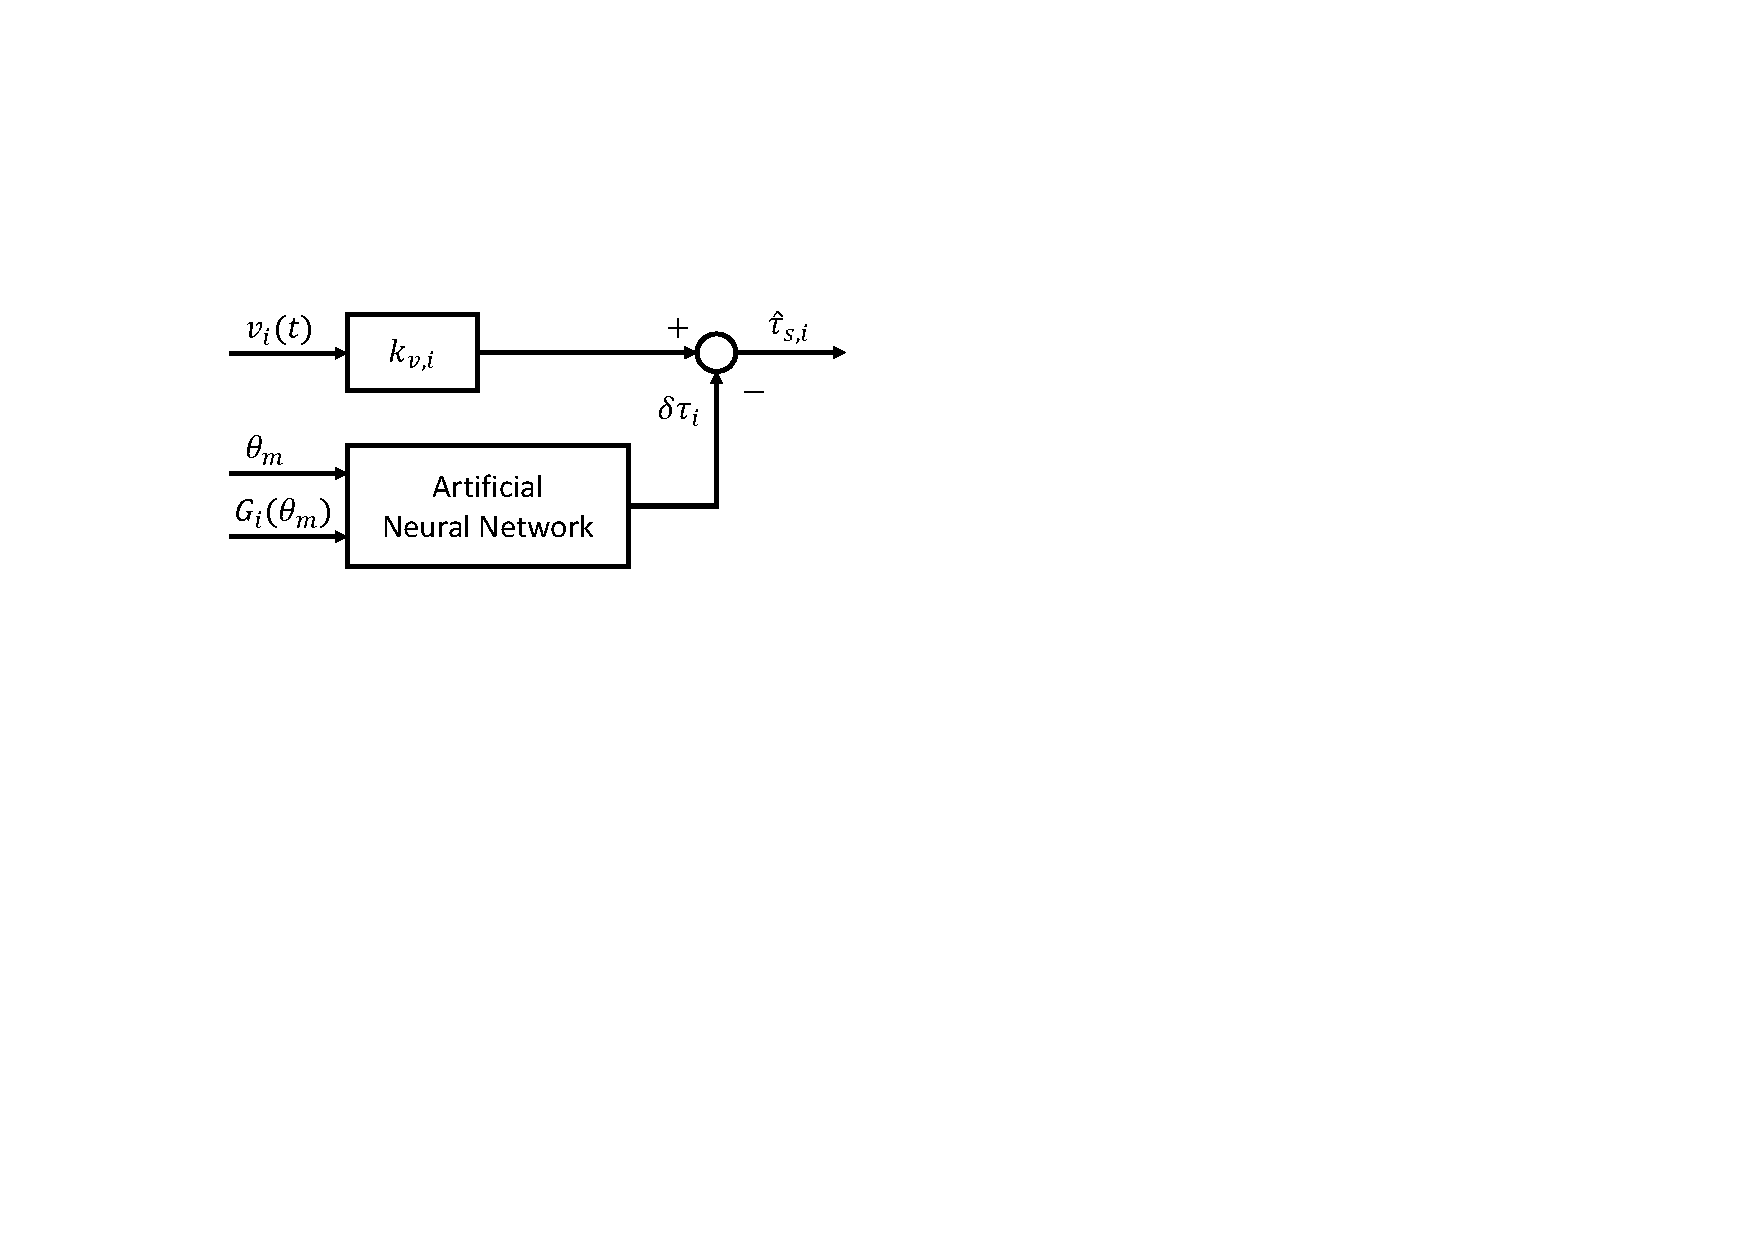
\includegraphics[width=0.7\columnwidth]{torqueEstimation}	
	\caption{The estimated sensor torque is obtained as the sum of sensor's reading and the predicted undesired non-linear term.}
	\label{fig:NN_schema}
\end{figure}
%\hl{QUi} As can be shown in the \figurename \ N, the introduction of the undesired term prediction induce a reduction in interaction force while a zero torque following control is implemented (see section N). Note that the force reduction is measured by the end effector force/torque sensor, while the  torque control use only the estimated torque using the sensor readings.
%%%%%%%%%%%%%%%%%%%%%%%%%%%%%%%%%%%%%%%%%%%%%%%%%%%%%%%%%%%%%%%%%%%%%%%%%%%%%%%%%%%%%%%%%%%%%%%%%%%%%%%%%%%%%%%%%%%%
%%%%%%%%%%%%%%%%%%%%%%%%%%%%%%%%%%%%%%%%%%%%%%%%%%%%%%%%%%%%%%%%%%%%%%%%%%%%%%%%%%%%%%%%%%%%%%%%%%%%%%%%%%%%%%%%%%%
\subsection{Control Hardware}
%\hldone{Done}
The control architecture of the Rehab-Exos is decentralized and based on the EtherCAT communication bus in order to guarantee both optimal signal to noise ratio in the acquisition of analogical signals, i.e. force sensors, and higher standards of safety.
The EtherCAT communication network consists of one master controller and four Ethercat Slave Controllers (ESC), one for each actuation joint.
The master controller is handled by Simulink Real-Time\texttrademark \ Operating System that executes the centralized control model at $2 \ kHz$ frequency.

Motors of the exoskeleton consist of three $170 \ VDC$ power supplied brush-less motors on the 1st, 2nd and 4th joint each one driven by programmable current driver and one $48 \ VDC$ power supplied DC motor on the 3th joint.  All of them are provided with one incremental encoder and one torque sensor.

Each ESC board is a custom control board featuring an up-to $72 \ Mhz$ ARM7 micro-controller, 4 14-bit DAC output interfaces (to set the reference of the current drives), 10 14-bit Analog-to-Digital Converter (ADC) channels (to acquire the torque signals through 2 Wheatstone full-bridge channels that are pre-amplified) and the EtherCAT ET1100 controller linking to double-port Ethernet interface.
%\begin{figure}[ht]
%	\centering
%	{\includegraphics[width=0.95\columnwidth]{\figpath{HWControlDiagram}}}
%	\caption{The decentralized control architecture}
%	\label{fig:ControlArchitecture}
%\end{figure}
%DIFDELCMD < %%%%%%%%%%%%%%%%%%%%%%%%%%%%%%%%%%%%%%%%%%%%%%%%%%%%%%%%%%%%%%%%%%%%%%%%%%%%%%%%%%%%%%%%%%%%%%%%%%%%%%%%%%%%%%%%%%%%
%%%%%%%%%%%%%%%%%%%%%%%%%%%%%%%%%%%%%%%%%%%%%%%%%%%%%%%%%%%%%%%%%%%%%%%%%%%%%%%%%%%%%%%%%%%%%%%%%%%%%%%%%%%%%%%%%%%%
\section{Dynamic model} \label{sec:dynamic_model}

\subsection{Single joint model} \label{Single joint model}
%\hldone{DONE}
The joints of the exoskeleton can be modeled with a lumped parameter model due to the elasticity of the harmonic drive speed reducer and torque sensor (for joints 1, 2 and 4) and of tendon transmission for joint 3. The used single joint model is a 2-mass with spring and damper (Fig. \ref{fig:exos_singlejoint_model}).
\par The single joint dynamics is formulated by the following equations:
\setlength{\arraycolsep}{0.0em}
\footnotesize
\begin{align}
%\label{eqn:dinamicaMotoreSingoloGiunto}
J_{m,i} \ddot{\theta}_{m,i}  + c_{m,i}\dot{\theta}_{m,i} + c_{t,i} (\dot{\theta}_{m,i}-\dot{\theta}_{j,i})  
{+}\:k_{t,i} ({\theta_{m,i}}-{\theta_{j,i}}) &= \tau_{m,i}+\tau_ {d,i} \nonumber	\\
\label{eqn:dinamicaLinkSingoloGiunto}
J_{l,i} \ddot{\theta}_{j,i}+c_{t,i} (\dot{\theta}_{j,i}-\dot{\theta}_{m,i})
+k_{t,i} ({\theta_{j,i}}-{\theta_{m,i}}) &= \tau_{l,i}	
\end{align}
\normalsize
\setlength{\arraycolsep}{5pt}
where referring to the i-th joint, $\theta_ {m,i}$ and $\theta_ {j,i}$ stand for motor and joint angles respectively, $k_{t,i}$ and $c_{t,i}$ are the stiffness and viscous coefficient of the transmission, that were experimentally characterized.
$J_{m,i}$ is motor inertia, $J_{l,i}$ is average link inertia considered as constant, $\tau_{m,i}$ is the motor torque, $\tau_{d,i}$ is a disturbance torque acting on the motor rotor  which accounts for internal friction and ripple effects of both motor and harmonic drive, while $\tau_{l,i}$ is the external torque acting directly on the output link. The $\tau_{l,i}$ torque accounts for the 
exogenous input due to the interaction  with the human, and endogenous input accounting for unmodeled non-linear effects, such as dynamic or gravity forces.
\begin{figure}[ht]
	\centering
	{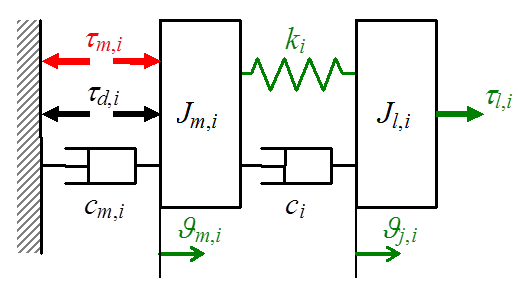
\includegraphics[width=0.5\columnwidth]{2massModel}}
	\caption{The 2-mass model for each joint}
	\label{fig:exos_singlejoint_model}
\end{figure}
%%%%%%%%%%%%%%%%%%%%%%%%%%%%%%%%%%%%%%%%%%%%%%%%%%%%%%%%%%%%%%%%%%%%%%%%%%%%%%%%%%%%%%%%%%%%%%%%%%%%%%%%%%%%%%%%%%%%
%%%%%%%%%%%%%%%%%%%%%%%%%%%%%%%%%%%%%%%%%%%%%%%%%%%%%%%%%%%%%%%%%%%%%%%%%%%%%%%%%%%%%%%%%%%%%%%%%%%%%%%%%%%%%%%%%%%%
\subsubsection{Experimental characterization of single joint performance}
%\hldone{DONE}
%\point{Insert here experimental data and procedures with indication of dynamic bandwidth}
As described in \ref{subsec:mechanicalDesign} the joint is equipped with a torque sensor that is a part of the transmission chain and is capable of measuring the elastic torque $\tau_{s,i}$, which acts between motor rotor and joint output link. The elastic sensor torque can be expressed by $\tau_{s,i} = k_{t,i} (\theta_{j,i}-\theta_{m,i})$. The joint dynamics can be re-written expliciting the $\tau_{s,i}$ readings starting from  $\tau_{s,i}$ definition, its 1st and 2nd derivatives and using the equations  \ref{eqn:dinamicaLinkSingoloGiunto}. It is obtained:
\begin{equation}
\label{eqn:dinamicaSensoreCoppia}
\ddot{\tau}_{s,i} + \frac{c_{t,i}}{J_i}\dot{\tau}_{s,i} + \frac{k_{t,i}}{J_i}\tau_{s,i}= \frac{k_{t,i}}{J_{l,i}}\tau_l + \frac{k_{t,i}}{J_{l,i}}\tau_g - \frac{k_{t,i}}{J_{m,i}}\tau_d - \frac{k_{t,i}}{J_{m,i}}\tau_m
\end{equation}
where $J_i = J_l J_m /(J_l+J_m)$. The natural frequency of this system is $\omega_n = \sqrt{k_{t,i} /J_i } /2\pi$. The natural frequency has been experimentally evaluated for a single joint in a test-rig analyzing the response of the $\tau_s$ when a chirp command is used for the $\tau_m$ motor torque. 
\par From Fig. \ref{fig:exos_singlejoint_model}, use of the Half-Power Bandwidth method returns c = 11.8Nms/rad as the overall damping coefficient of the flexible joint (this value has also been validated via the Logarithmic Decrement method).
\begin{figure}[ht]
	\centering
	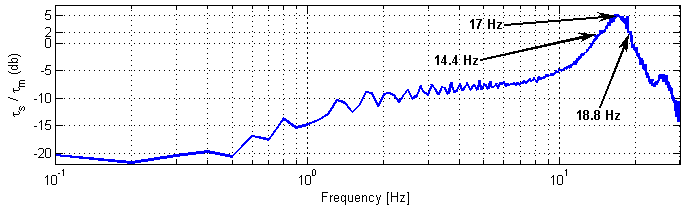
\includegraphics[width=1\columnwidth]{OpenLoopJointBode}
	\caption{Experimental open-loop response (Bode magnitude plot) of joints 1,2 and 4: joint sensor torque vs. motor torque command.}
	\label{fig:OpenLoopJointBode}
\end{figure}
Considering the exoskeleton, every joint see a link inertia that depends on the pose so the natural frequency of each joint depends on the pose of the exoskeleton. 
Considering an average link inertia, it can be obtained the natural frequency for each joint elastic transmission. Results are shown in the \tablename \ \ref{tab:naturalFrequencies}.
%\begin{table}[!t]
%	\renewcommand{\arraystretch}{1.3}
%	\caption{The natural frequency of the joints}
%	\label{tab:naturalFrequencies}
%	\centering
%	\begin{tabular}{|c|c|c|}
%		\hline
%		\bfseries Joint & \bfseries Avg. link inertia [$Kg/m^2$] & \bfseries Natural freq. [$Hz$]\\
%		\hline\hline
%		1 & 0.9639 & 19.3930\\
%		\hline
%		2 & 1.11 & 18.3501\\
%		\hline
%		4 & 0.1925 & 39.6797\\
%		\hline
%	\end{tabular}
%\end{table}
\begin{table}[!t]
	\renewcommand{\arraystretch}{1.3}
	\caption{The natural frequency of the joints}
	\label{tab:naturalFrequencies}
	\centering
	\begin{tabular}{c c c}
		\hline \hline
		\bfseries Joint & \bfseries Avg. link inertia [$Kg/m^2$] & \bfseries Natural freq. [$Hz$]\\
		\hline
		1 & 0.9639 & 19.3930\\
		2 & 1.11 & 18.3501\\
		4 & 0.1925 & 39.6797\\
		\hline \hline
	\end{tabular}
\end{table}
For all these three joints the motor inertia is the same and it is equivalent to $3.742 \ Kg/m^2$


%%%%%%%%%%%%%%%%%%%%%%%%%%%%%%%%%%%%%%%%%%%%%%%%%%%%%%%%%%%%%%%%%%%%%%%%%%%%%%%%%%%%%%%%%%%%%%%%%%%%%%%%%%%%%%%%%%%%
%%%%%%%%%%%%%%%%%%%%%%%%%%%%%%%%%%%%%%%%%%%%%%%%%%%%%%%%%%%%%%%%%%%%%%%%%%%%%%%%%%%%%%%%%%%%%%%%%%%%%%%%%%%%%%%%%%%%
%%%%%%%%%%%%%%%%%%%%%%%%%%%%%%%%%%%%%%%%%%%%%%%%%%%%%%%%%%%%%%%%%%%%%%%%%%%%%%%%%%%%%%%%%%%%%%%%%%%%%%%%%%%%%%%%%%%%
%%%%%%%%%%%%%%%%%%%%%%%%%%%%%%%%%%%%%%%%%%%%%%%%%%%%%%%%%%%%%%%%%%%%%%%%%%%%%%%%%%%%%%%%%%%%%%%%%%%%%%%%%%%%%%%%%%%%
\subsection{Multiple joints model} \label{Full dynamics model}

Given the single joint two-mass model, the dynamic model of the whole exoskeleton can be formulated in matrix form as follows:
\setlength{\arraycolsep}{0.0em}


%\footnotesize

\begin{equation}
\left \{
\begin{IEEEeqnarraybox}[][c]{l}
\vectm{J_m}    \vectm{D} \vects{\ddot{\theta}_m} + \vectm{B_m  D} \vects{\dot{\theta}_m}  + \vectm{C_t}  ( \vectm{D} \vects{\dot{\theta}_m} - \vects{\dot{\theta}_j} )+ 
\:\vectm{K_t}  ( \vectm{D} \vects{\theta_m}- \vects{\theta_j} ) =  \\ \vects{\tau_m} +\vects{\tau_d}   \\
\vectm{M}(\vects{\theta_j}) \vects{\ddot{\theta}_j}  + \vectm{C}( \vects{\dot{\theta}_j}, \vects{\theta_j})   \vects{\dot{\theta}_j} +   \vectm{C_t}  ( \vects{\dot{\theta}_j} - \vectm{D} \vects{ \dot{\theta}_m} )
{+}\: \vectm{K_t}  ( \vects{\theta_j} - \vectm{D}\vects{\theta_m} ) + \\ + \vects{G}( \vects{\theta_j}) = \vectm{J}^T \vects{F_h}
\label{eqn:dinamicaLinkMultiGiunto}
\end{IEEEeqnarraybox}
\right . %\label{eqn:dinamicaMotoreMultiGiunto}
\end{equation}
%\label{eqn:dinamicaMotoreMultiGiunto} 
\normalsize
\setlength{\arraycolsep}{5pt}



%\begin{eqnarray}
%\label{eqn:dinamicaMotoreMultiGiunto}
%\vectm{J_m}    \vectm{D} \vects{\ddot{\theta}_m} + \vectm{B_m  D} \vects{\dot{\theta}_m}  + \vectm{C_t}  ( \vectm{D} \vects{\dot{\theta}_m} - \vects{\dot{\theta}_j} )+ 
%\:\vectm{K_t}  ( \vectm{D} \vects{\theta_m}- \vects{\theta_j} ) =  \nonumber\\ \vects{\tau_m} +\vects{\tau_d}
%\end{eqnarray}


%\begin{eqnarray}
%\label{eqn:dinamicaLinkMultiGiunto}
%\vectm{M}(\vects{\theta_j}) \vects{\ddot{\theta}_j}  + \vectm{C}( \vects{\dot{\theta}_j}, \vects{\theta_j})   \vects{\dot{\theta}_j} +   \vectm{C_t}  ( \vects{\dot{\theta}_j} - \vectm{D} \vects{ \dot{\theta}_m} )+ 
%{+}\: \vectm{K_t}  ( \vects{\theta_j} - \vectm{D}\vects{\theta_m} ) + \nonumber\\ + \vects{G}( \vects{\theta_j}) = \vectm{J}^T \vects{F_h}
%\end{eqnarray}


%where $\vectm{D}$ is a diagonal matrix modeling the reduction factor introduced by joint speed reducers, $\vectm{J_m}$ and $\vectm{B_m}$ are diagonal matrices modeling inertia and viscous friction at motor respectively; $\vectm{K_t}$ and $\vectm{C_t}$ are diagonal matrices modeling stiffness and damping associated to the elastic transmission; $\vects{G}$ models the effects of gravity force on links.
where $\vectm{J_m}$, $\vectm{B_m}$, $\vectm{D}$, $\vectm{K_t}$ and $\vectm{C_t}$ are diagonal matrices.  $\vectm{J_m}$ and $\vectm{B_m}$ model inertia and viscous friction at motor respectively, while $\vectm{K_t}$ and $\vectm{C_t}$ model stiffness and damping associated to the elastic transmission and $\vectm{D}$ models  the transmission reduction factor introduced by joint gearheads; $\vects{G}$ models the effects of gravity force on links.
$\vects{F_h}$ are the external  forces  acting on the system  due to human interaction  and the respective joint torques are computed by multiplying them by the transposed Jacobian matrix  $J^T$ evaluated in the actual exoskeleton configuration. The multi-joint model introduces cross-coupling among joints and non-linearities, with terms $ \vectm{C}( \vects{\dot{\theta}_j}, \vects{\theta_j})  $ that models Coriolis effects and $\vectm{M}(\vects{\theta_j}) $ that represents links inertia.

By taking into account that
that the real dynamics has terms  $\vectm{M}(\vects{\theta_j}) $  and $ \vectm{C}( \vects{\dot{\theta}_j}, \vects{\theta_j}) $ depending on the actual joint configuration, the first term can be decoupled into a diagonal constant component and a variable component as follows:
\begin{equation}
\vectm{M }  \vects{\ddot{\theta}_j}=
\overline{\vectm{M} } \vects{\ddot{\theta}_j} + \Delta \vectm{M} (\vects{\theta_j}) \vects{\ddot{\theta}_j} 
\label{eq:InertialComponent}
\end{equation}
and introducing  the following variable substitution for joint torque $\vects{\tau_s}$
\footnotesize
\begin{equation}
\left \{
\begin{aligned}
\vects{\tau_s} & = - \vectm{K_t}  ( \vectm{D} \vects{\theta_m}- \vects{\theta_j} ) \\
\vects{\dot{\tau_s}} & = - \vectm{K_t}  ( \vectm{D}  \vects{\dot{\theta}_m} - \vects{\dot{\theta}_j} ) \\
\vects{\ddot{\tau_s}} & = - \vectm{K_t}  ( \vectm{D}  \vects{\ddot{\theta}_m} - \vects{\ddot{\theta}_j} ) \\
\end{aligned}
\right .
\label{eq:taus}
\end{equation}
\normalsize

the dynamics equations can be reformulated as follows:

%\footnotesize
\begin{equation}
\left \{
\begin{IEEEeqnarraybox}[][c]{l}
\vectm{ J_m  D } \vects{ \ddot{\theta}_m} + \vectm{B_m D}\vects{\dot{\theta}_m}  = \vectm{K_t}^{-1} \vectm{C_t}\vects{ \dot{\tau}_s} + \vects{\tau_s} + \vects{u} + \vects{\tau_d} \\
\vects{\ddot{\tau}_s}  + \vectm{C_t J_i}^{-1} \vects{\dot{\tau}_s} + \vectm{K_t J_i}^{-1} \vects{\tau_s} = \vectm{K_t   J_m}^{-1}  \vectm{B_m D}\vects{\dot{\theta}_m}+  \\
{+}\:\overline{\vectm{M}}^{-1} \vectm{K_t J}^T \vects{F_l} - \vectm{K_t J_{m}}^{-1} \vects{\tau_d} - \vectm{K_t J_m}^{-1} \vects{u}
\end{IEEEeqnarraybox}
\right .
\label{eq:taus}
\end{equation}
\normalsize
%\label{eq:dynamics_eq1}
%\label{eq:dynamics_eq2}
\setlength{\arraycolsep}{0.0em}


\setlength{\arraycolsep}{5pt}

where  $\vects{u}$ represents the actual control command and the external  disturbance forces  have been collected within the external load  force  $\vects{F_l}$  term (see Appendix I for detailed derivation of terms).

This form of the dynamics equation is useful for defining a full-state feedback control law and an optimal observer for the estimation of joint torque.

%\begin{multline}
%%\begin{aligned}
% \overline{M}K_t^{-1}\vects{\ddot{\tau_s}} + K_t^{-1}  C_t (I+  \overline{M} J_m^{-1}) ]\vects{\dot{\tau_s}}  +\\
% + (I+   \overline{M} J_m^{-1})\vects{\tau_s}  =  \overline{M}(\vects{q_j}) J_m^{-1}  B_m    D  \dot{\vects{\theta}}_m   \\ +  J^T  \vects{F_{l}}-\overline{M} J_m^{-1} \vects{u}- \overline{M} J_{m}^{-1}\vects{\tau_d}
%%\end{aligned}
%\label{eqdyn}
%\end{multline}


%so if 
%then it follows that 
%$$[I+  \overline{M} J_m^{-1}]=\overline{M} J_i^{-1}$$
%then by replacing $J_i$ in equation 	\eqref{eqdyn}, we find the  set of dynamic equations: 



%%%%%%%%%%%%%%%%%%%%%%%%%%%%%%%%%%%%%%%%%%%%%%%%%%%%%%%%%%%%%%%%%%%%%%%%%%%%%%%%%%%%%%%%%%%%%%%%%%%%%%%%%%%%%%%%%%%%
%%%%%%%%%%%%%%%%%%%%%%%%%%%%%%%%%%%%%%%%%%%%%%%%%%%%%%%%%%%%%%%%%%%%%%%%%%%%%%%%%%%%%%%%%%%%%%%%%%%%%%%%%%%%%%%%%%%%
%\subsection{(?) Different models for interaction torque control}
%
%\label{Centralized interaction torque control}

%%%%%%%%%%%%%%%%%%%%%%%%%%%%%%%%%%%%%%%%%%%%%%%%%%%%%%%%%%%%%%%%%%%%%%%%%%%%%%%%%%%%%%%%%%%%%%%%%%%%%%%%%%%%%%%%%%%%
%%%%%%%%%%%%%%%%%%%%%%%%%%%%%%%%%%%%%%%%%%%%%%%%%%%%%%%%%%%%%%%%%%%%%%%%%%%%%%%%%%%%%%%%%%%%%%%%%%%%%%%%%%%%%%%%%%%%

%%%%%%%%%%%%%%%PROBLEM HERE INSERTION POINT %%%%%%%%%%%%%%%%%%%%%%%%%%%%%%%%



\subsubsection{Joint acceleration estimation}  \label{acc_observer}

The full dynamics model of the exoskeleton  is dependent on the acceleration of each joint. In order to estimate and compensate for the dynamics of the device, an observer for the joint acceleration has been designed. 
The observer estimates the acceleration from motor encoder $\theta_{m,i}$,  joint torque $\tau_{s,i}$ and the imposed control torque $\tau_{m,i}$.
$\tau_{s,i}$ is the torque measured by the sensor at the joint and can be expressed as in equation (\ref{eq:taus}).

The acceleration can be estimated starting from a model of the actuation group (motor and gearhead), in particular by modeling the torque acting on the actuation group as $\tau_{m,i}-\tau_{s,i}$ and by considering the losses as a static and a velocity-dependent viscous friction. Thus, the acceleration can be estimated as:



%\begin{equation}
%\left \{
%\begin{aligned}
%\ddot{\theta}_{m,i}=0 \quad for -\tau_A<\tau_{m,i}-\tau_s<\tau_A \\
%\ddot{\theta}_{m,i}=\frac{\tau_{m,i}-\tau_{s,i}-k_f\dot{\theta}_{m,i}}{J_{m,i}}
%\end{aligned}
%\right .
%\label{tau_acc}
%\end{equation}

\begin{equation}
\left \{
\begin{aligned}
\ddot{\theta}_{m,i} & =0 \quad \text{for} -\tau_{A,i}<\tau_{m,i}-\tau_{s,i}<\tau_{A,i} \\
\ddot{\theta}_{m,i} & =\frac{\tau_{m,i}-\tau_{s,i}  -c_{m,i}\dot{\theta}_{m,i}}{J_{m,i}} \quad \text{ otherwise}
\end{aligned}
\right .
\label{tau_acc}
\end{equation}

where $\tau_{A,i}$ is the static friction torque and $c_{m,i}$ is the dynamic friction coefficient that were experimentally evaluated.
The torque saturation effects due to power supply voltage limits are modeled as:

\begin{equation}
k_c\frac{-V_{max}-k_v\dot{\theta}_{m,i}}{R}<\tau_{m,i}<k_c\frac{V_{max}-k_v\dot{\theta}_{m,i}}{R}
\label{torque_saturation}
\end{equation}
depending on the electric constants of each motor, and in particular  where $k_c$ is the associated torque constant, $k_v$ is the velocity constant, $R$ is the winding terminal resistance and $V_{max}$ is the maximum supply voltage to the motor.
An optimum Kalman observer has been used to estimate the acceleration term $\ddot{\theta}_{m,i}$ and a diagram of the estimation of acceleration by using control and measured torques is shown in Fig. \ref{fig:acc_estimation}.

\begin{figure}[htb]
	\centering
	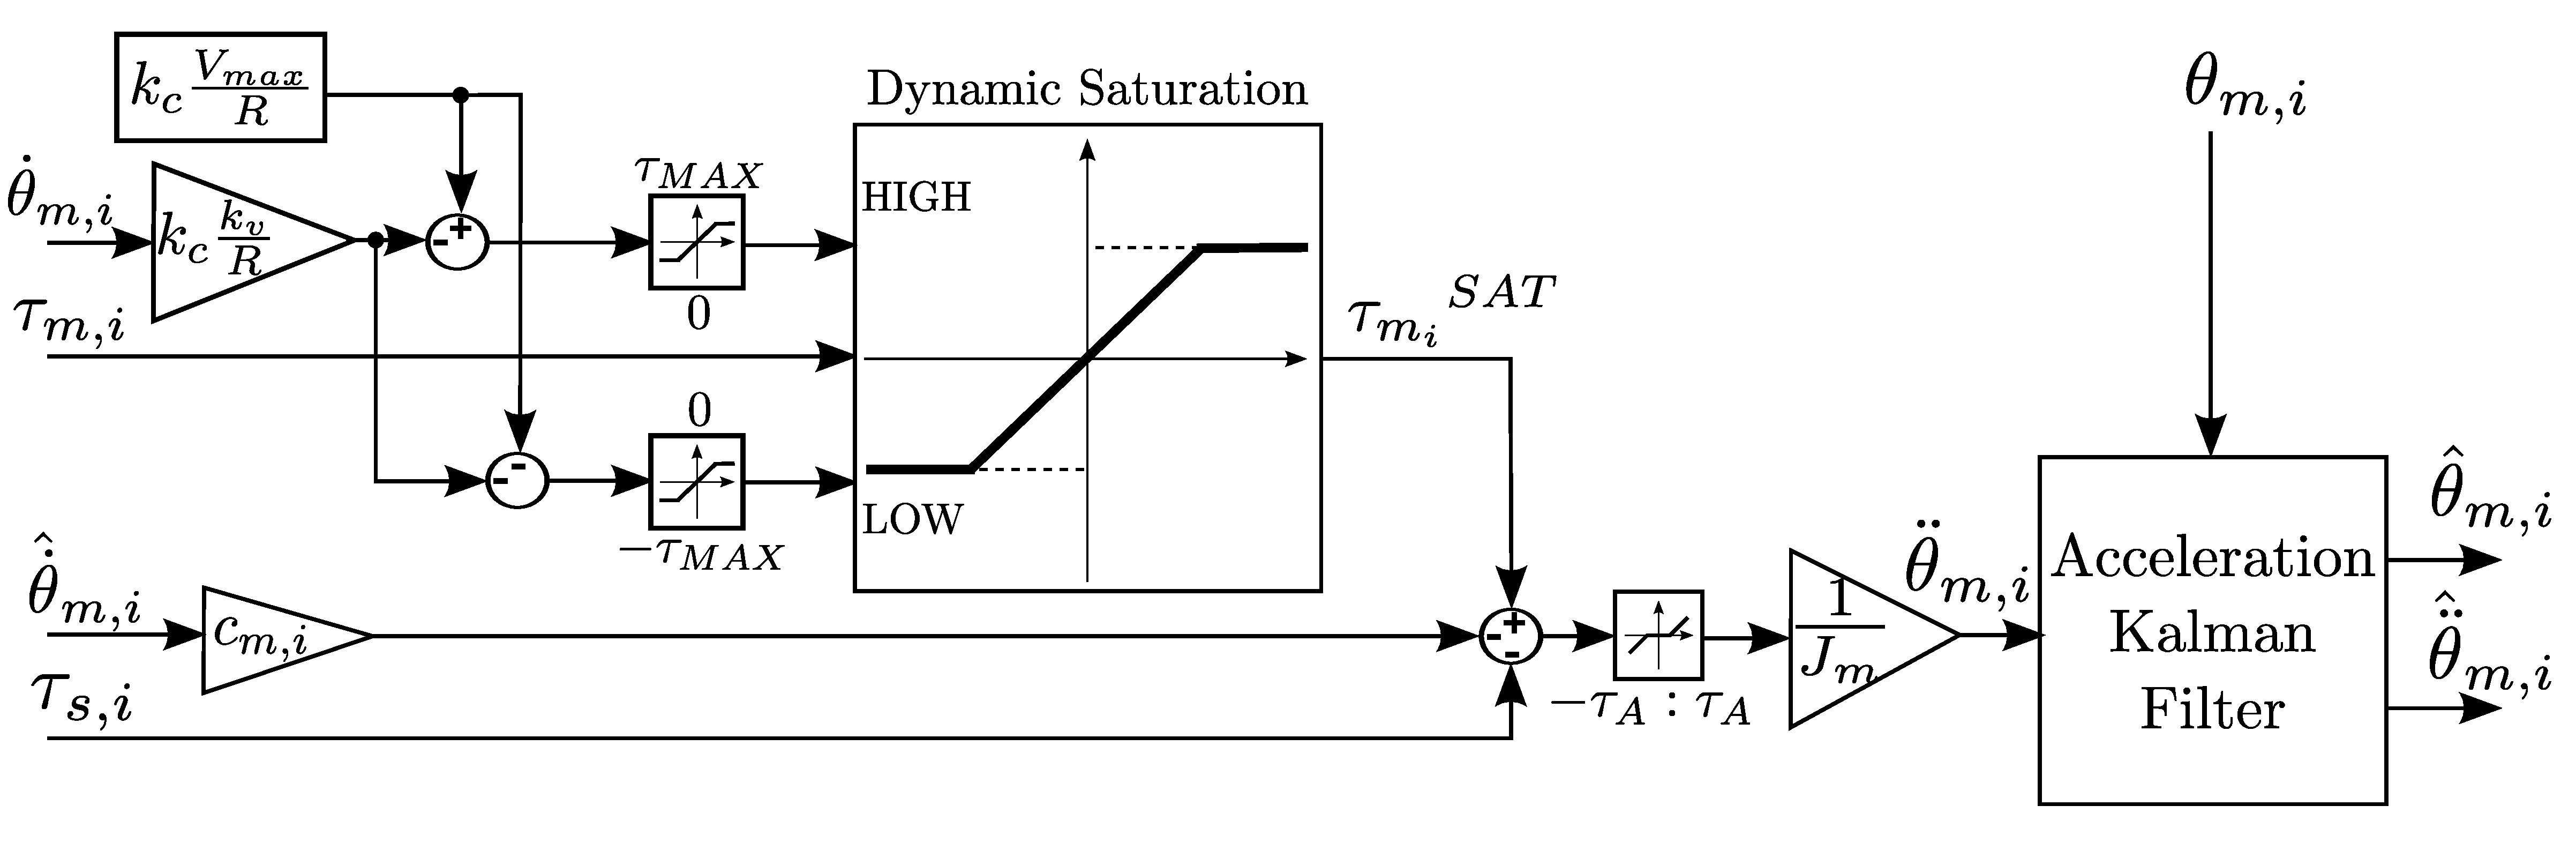
\includegraphics[width=1.0\columnwidth]{DynamicSaturation}
	\caption{Estimation of the acceleration from torque measurement}
	\label{fig:acc_estimation}
\end{figure}
%
%While $\tau_{s,i}$ is directly measured by the joint torque sensor  and $\tau_{m,i}$ is derived from motor command,
%an optimum Kalman observer has been used to estimate the acceleration term $\ddot{\theta}_{m,i}$
%from direct position measurements.
%

The model can be expressed in the state variable form as follows:
%

\begin{equation}
\left \{
\begin{aligned}
\vects{\dot{x}}=\vectm{A}\vects{x} + \vectmm{\Gamma}\vects{d} \\
\vects{y}=\vectm{C}\vects{x}
\end{aligned}
\right .
\end{equation}
%
where
%
\begin{equation}
\begin{aligned}
\vects{x}=\vectlong{ {\theta_{m,i}} \\ \dot{\theta}_{m,i} \\ \ddot{\theta}_{m,i}}
\vectm{A}=\mat{0 & 1 & 0  \\
	0 & 0 & 1 \\
	0 & 0 & 0 }
\vectmm{\Gamma}=\vectlong{ 0 \\ 0 \\ 1}
\vectm{C}=\mat{1 & 0 & 0  \\
	0 & 0 & 1} 
\end{aligned}
\end{equation}
%
and $d$ is the process noise.

The observer can be formulated as:
%
\begin{equation}
\vects{\dot{\hat{x}}}=\vectm{A}\vects{\hat{x}}+\vectm{L}(\vects{y}-\vectm{C}\vects{\hat{x}})
\end{equation}
%
where L is the gain matrix of the observer. A scheme of the observer is depicted in figure (\ref{fig:block_acc_observer}). 
%
\begin{figure}[htb]
	\centering
	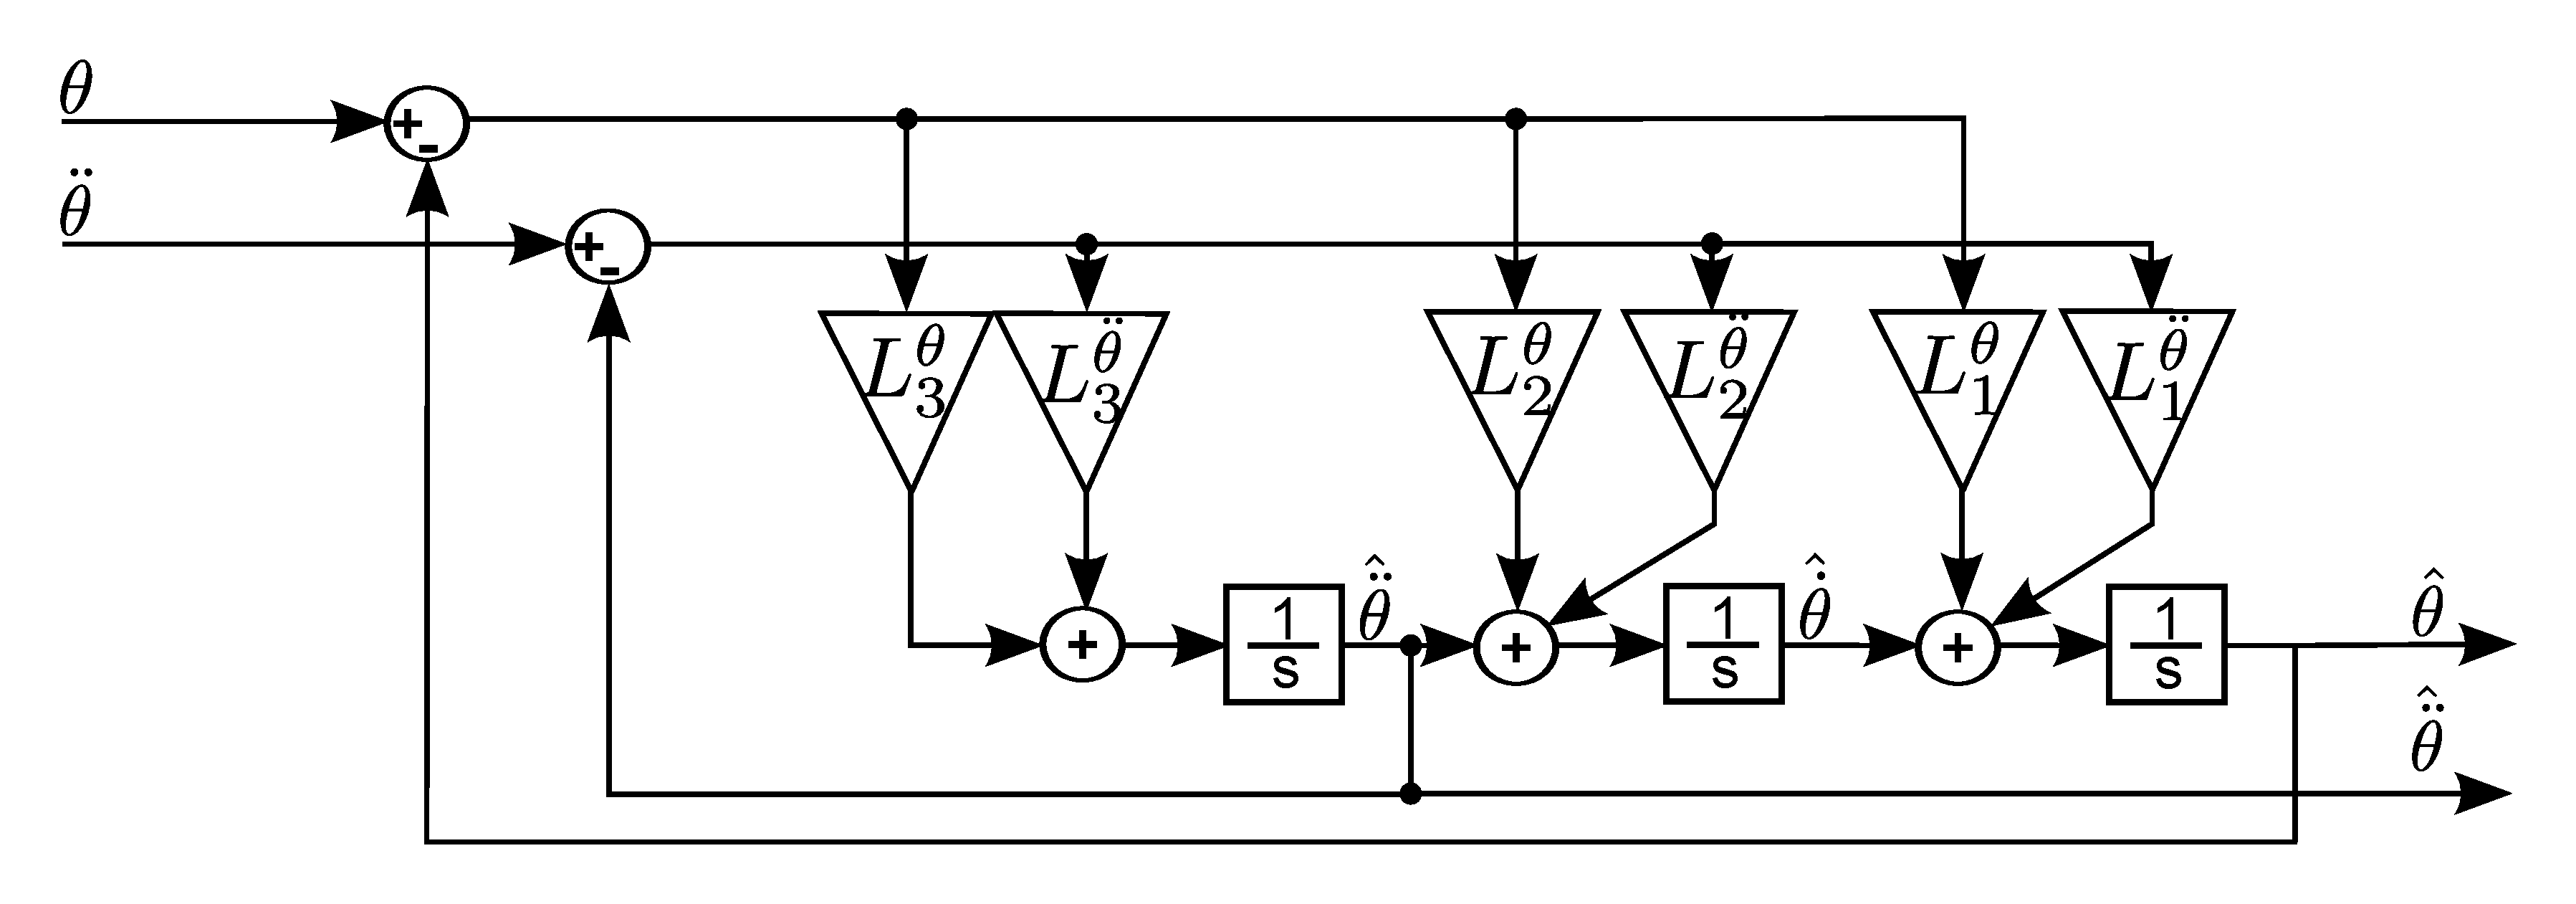
\includegraphics[width=1.0\columnwidth]{aKalmanFilter}
	\caption{Block diagram of the acceleration observer}
	\label{fig:block_acc_observer}
\end{figure}

As an example, the comparison between the real-time estimated acceleration (red dotted line) and the off-line calculated acceleration (blue solid line) for the first two joints is shown in figure \ref{fig:acceleration_validation}.
%
\begin{figure}[htb]
	\centering
	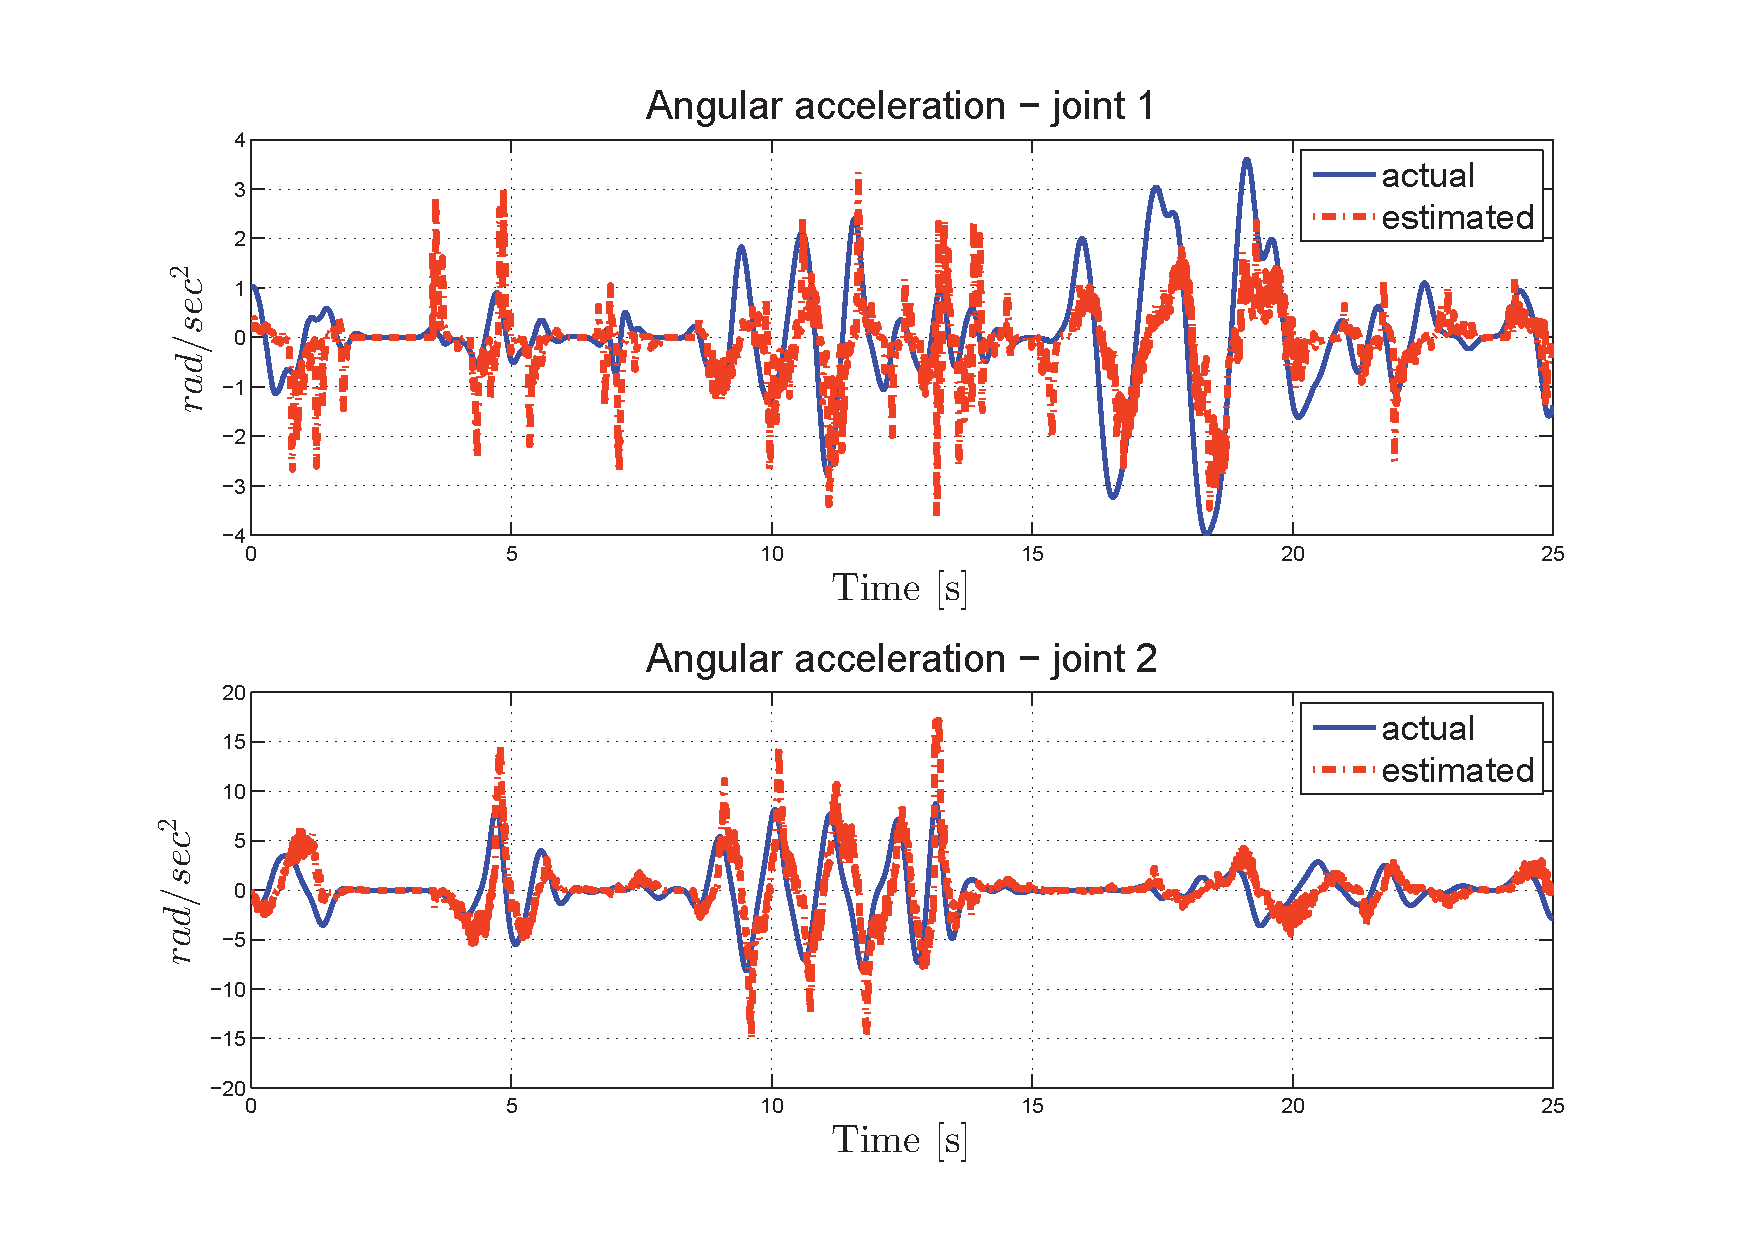
\includegraphics[width=1.0\columnwidth]{a1_a2_vs_ak1_ak2.pdf}
	\caption{Comparison between the estimated and actual acceleration}
	\label{fig:acceleration_validation}
\end{figure}

%%%%%%%%%%%%%%%%%%%%%%%%%%%%%%%%%%%%%%%%%%%%%%%%%%%%%%%%%%%%%%%%%%%%%%%%%%%%%%%%%%%%%%%%%%%%%%%%%%%%%%%%%%%%%%%%%%%%
%%%%%%%%%%%%%%%%%%%%%%%%%%%%%%%%%%%%%%%%%%%%%%%%%%%%%%%%%%%%%%%%%%%%%%%%%%%%%%%%%%%%%%%%%%%%%%%%%%%%%%%%%%%%%%%%%%%%

\subsubsection{Dynamics compensation} \label{Dynamics compensation}

% Spiegare da dove viene fuori la storia della compensazione, dato che taul non è osservabile e che per imporre il meglio possible la taul mediante taum c'è bisogno di compensare\hl{TO DO}
As reported by equation (\ref{eq:extraForces}), the torques measured by joint sensors are due to the human force and any load applied on the links ($\vects{F_l}$). To have a good estimation of human forces by torque sensors, it is necessary to remove from torque measurements the gravity and dynamics loads applied to the links. The gravity contribution  depends only on the pose of the exoskeleton and it can be calculated by the position signals provided by the motor encoders. The gravitational term is already compensated in feed-forward by the term $\hat{\vectm{G}}(\vectm{D}\vects{\hat{\theta}_m})$ in $\vects{\tau_{m}}$,
except for the term $\delta \vects{g}$.
On the other side, the dynamics contribution depends both on the pose and the acceleration and velocity of the links, which are not directly provided by any sensor, but are provided in first approximation as $\vectm{D} \vects{\hat{\ddot{\theta}}_m}$  by the observer described in section \ref{acc_observer}.

The dynamics torques due to the links inertia and measured by the joint torque sensors can be so estimated as the sum of the inertial contribute and the Coriolis effect:

\begin{equation}
\vects{\hat{\tau}_{dyn}}  \eqsim \hat{\vectm{M}}(\vectm{D} \vects{\theta_m}) \vectm{D} \vects{\ddot{\theta}_m}+\hat{\vectm{C}}(\vectm{D} \vects{\theta_m},\vectm{D} \vects{\dot{\theta}_m})\vectm{D} \vects{\dot{\theta}_m}
\end{equation}

where matrices $\hat{\vectm{M}}$ and $\hat{\vectm{C}}$ are calculated taking into account for each joint the inertia of the parts supported by the torque sensor, discarding the inertia of the actuator of the joint.

The estimated dynamic torques are then used to compensate the dynamic effects of the link: the compensation torques $\alpha \vects{\hat{\tau}_{dyn}}$, with $0<\alpha<1$, are a percentage of the estimated torques $\vects{\hat{\tau}_{dyn}}$. The compensation torques are added to the desired torques $\vects{\tau_s^D}$ as input to the state feedback controller and feed-back with the estimated torque $\vects{\hat{\tau}_s}$. 

%%%%%%%%%%%%%%%%%%%%%%%%%%%%%%%%%%%%%%%%%%%%%%%%%%%%%%%%%%%%%%%%%%%%%%%%%%%%%%%%%%%%%%%%%%%%%%%%%%%%%%%%%%%%%%%%%%%%
%%%%%%%%%%%%%%%%%%%%%%%%%%%%%%   Full state feedback controller    %%%%%%%%%%%%%%%%%%%%%%%%%%%%%%%%%%%%%%%%%%%%%%%%%
%%%%%%%%%%%%%%%%%%%%%%%%%%%%%%%%%%%%%%%%%%%%%%%%%%%%%%%%%%%%%%%%%%%%%%%%%%%%%%%%%%%%%%%%%%%%%%%%%%%%%%%%%%%%%%%%%%%%
%%%%%%%%%%%%%%%%%%%%%%%%%%%%%%%%%%%%%%%%%%%%%%%%%%%%%%%%%%%%%%%%%%%%%%%%%%%%%%%%%%%%%%%%%%%%%%%%%%%%%%%%%%%%%%%%%%%%
%%%%%%%%%%%%%%%%%%%%%%%%%%%%%%%%%%%%%%%%%%%%%%%%%%%%%%%%%%%%%%%%%%%%%%%%%%%%%%%%%%%%%%%%%%%%%%%%%%%%%%%%%%%%%%%%%%%%
%\section{Joint Torque Feedback Controllers: Full state feedback, Basic feedback and Passivity-Based feedback}
%DIFDELCMD < \section{Full state, basic and passivity-based feedback controllers} 
\label{sec:Full_state_feedback_controllers}

From the full dynamic model of the exoskeleton, a novel  full state feedback control law   was  derived and implemented. This control law is  identified in the following with the acronym JTFC1  and  explained in subsection \ref{subsec:JTFC1}.
To implement the control, the state of the system and, more in particular, the joint torque was estimated through a Kalman Filter described in  subsection \ref{subsec:kalmanTorque}.
To evaluate the performance of  the proposed full state feedback control,  two other torque controls inspired to existing joint torque controls available in literature have been implemented, identified respectively with the acronyms JTFC2 and JTFC3.
% We searched for torque controls designed for joint torque-based robots with a joint structure similar to the Rehab-Exos one.
\par The JTFC2, presented in subsection \ref{subsec:JTFC2}, is based on a  torque control   for  single joint based on torque sensor first  introduced by Hashimoto \cite{hashimoto1998experimental}. In order to compare the basic torque control with our full state feedback control, the Hashimoto formulation was extended and generalized to a multi-dof case. 
\par The JTFC3, reported in subsection \ref{subsec:JTFC3}, was inspired to the passivity-based control law \cite{kugi2008passivity}
implemented for the DLR Light Weight Robot III (LWR III)   that guarantees the passivity of the controlled system. The DLR LWR III shows a joint design compatible with the Rehab-Exos one, since both systems make use of the joint torque sensor to estimate the interaction torques/forces with the environment/human.


%%%%%%%%%%%%%%%%%%%%%%%%%%%%%%%%%%%%%%%%%%%%%%%%%%%%%%%%%%%%%%%%%%%%%%%%%%%%%%%%%%%%%%%%%%%%%%%%%%%%%%%%%%%%%%%%%%%%
%%%%%%%%%%%%%%%%%%%%%%%%%%%%%%%%%%%%%%%%%%%%%%%%%%%%%%%%%%%%%%%%%%%%%%%%%%%%%%%%%%%%%%%%%%%%%%%%%%%%%%%%%%%%%%%%%%%%
\subsection{An optimal observer for estimation of joint torque}\label{subsec:kalmanTorque}
Since the correct state estimation  is essential for the design of a full-state feedback joint-torque controller, the knowledge of the interaction torques between the human arm and the exoskeleton are required for  torque control implementation. The joint torque sensor provides a raw measurement $\tau_{s,i}$ that can be used together with the measured joint position $\theta_{m,i}$ to filter the sensed torque and to estimate the full system state, given by $[\tau_{s,i},\ \dot{\tau}_{s,i},\ \theta_{m,i},\ \dot{\theta}_{m,i},\ \tau_{d,i},\ \tau_{l,i}]$, where $\vects{\tau_l}=\vectm{J}^T \vects{F_l}$. 
Thus, a full-state Kalman filter has been designed to clean out both  $\theta_{m,i}$ from quantization noise $w_{\theta,i}$ and $\tau_{s,i}$ from measurement noise $w_{\tau,i}$, as well as to estimate the remaining variables.
%
\par 
Following \cite{vertechy2012interaction}, the dynamics of the two state components $\tau_{d,i}$ and $\tau_{l,i}$ can be modeled as two distinct Wiener processes (i.e. as two distinct non-stationary random processes) $\dot{\tau}_{d,i}=v_{d,i}$ and $\dot{\tau}_{l,i}=v_{l,i}$. Starting from equations (\ref{eq:dynamics_eq1},\ref{eq:dynamics_eq2}) the following meta-system can be derived:
%


%%%%%%DA VERIFICARE COSA SUCCESSO

\begin{equation}
\left \{
\begin{aligned}
\vects{\dot{\tau}_i} &=\vectm{A_i}\vects{\tau_i}+\vectm{B_i}\vects{\tau_{m,i}}+\vectmm{\Gamma}\vects{v_i} \\
		\vects{y_i} &=\vectm{C}\vects{\tau_i}+\vects{w_i}
		\end{aligned}
		\right .
		\label{eq:metasystem}
		\end{equation}
		%
		where $\vects{\tau_i}^T=[ \dot{\tau}_{s,i}\ \tau_{s,i}\ \dot{\theta}_{m,i}\ \theta_{m,i}\  \tau_{l,i} \tau_{d,i}\ ]$ is the meta-state vector, $\vects{v_i}^T=[ v_{l,i}\ v_{d,i} ]$ is the vector of process noises with variances $V_{l,i}$ and $V_{d,i}$, $\vects{w_i}^T=[ w_{\tau,i}\ w_{\theta,i} ]$ is the vector of measurement noises with variances $W_{l,i}$ and $W_{d,i}$, whereas:
		%
		\begin{equation}
		\begin{aligned}
		\vectm{A_i}=\mat{ \frac{-c_{t,i}}{J_i}  & \frac{-k_{t,i}}{J_i}& \frac{k_{t,i}b_{m,i}}{J_{m,i}} & 0 & \frac{ k_{t,i}}{J_{l,i}} &  \frac{-k_{t,i}}{J_{m,i}} \\
			1 & 0 & 0 & 0 & 0 & 0\\
			\frac{c_{t,i}}{  k_{t,i} J_{m,i} }&  \frac{1}{J_{m,i}} &  \frac{ -b_{m,i}}{J_{m,i}} & 0 & 0 &  \frac{1}{J_{m,i}}\\
			0 & 0 & 1 & 0 & 0 & 0\\
			0 & 0 & 0 & 0 & 0 & 0\\
			0 & 0 & 0 & 0 & 0 & 0} \\
		\vectm{B_i}=\vectlong{ \frac{ -k_{t,i}}{J_{m,i}} \\ 0 \\ \frac{1}{J_{m,i}} \\ 0 \\ 0 \\ 0}  \quad
		\vectmm{\Gamma}=\mat{ 0 & 0 \\ 0 & 0 \\ 0 & 0 \\ 0 & 0 \\ 1 & 0 \\ 0 & 1} \quad
		\vectm{C}=\mat{0 & 0 \\  1 & 0 \\  0 & 0  \\
			0 & 1 \\  0 & 0 \\ 0 & 0 } 
		\end{aligned}
		\label{stateobserver}
		\end{equation}
		%%%%%%%%%%%%%%%%%%%%%%%%%%%%%%%%%%%%%%%%%%%%%%%%%%%%%%%%%%%%%%%%%%%%%%%%%%%%%%%%%%%%%%%%%%%%%%%%%%%%%%%%%%%%%%%%%%%%
		%%%%%%%%%%%%%%%%%%%%%%%%%%%%%%%%%%%%%%%%%%%%%%%%%%%%%%%%%%%%%%%%%%%%%%%%%%%%%%%%%%%%%%%%%%%%%%%%%%%%%%%%%%%%%%%%%%%%


	\subsection{A full state feedback controller (JTFC1)} \label{subsec:JTFC1}
	
	The proposed control law is based on the full state obtained from the state  observer described by (\ref{eq:metasystem})  (\ref{stateobserver}), where the input control $\vects{u}$ is splitted up into one term $\vects{u_f}$, which implement control force behavior, and another term $\vects{u_g}$, which acts as a gravity compensation
	
	\begin{equation}
	\label{generic_control_law1}
	\begin{aligned}
	\vects{u} &= \vects{u_f} + \vects{u_g}
	\end{aligned}
	\end{equation}
	
The two above terms are expressed as:
	
	\setlength{\arraycolsep}{0.0em}
	
	\begin{eqnarray}{ll}
			\label{eq:JTCF1_control_law_a}
				\vects{u_g} &= \vects{G}(\vectm{D}\vects{\hat{\theta}_m}) \\
			\vects{u_f} &  =- \vectm{J_m} \vectm{K_t}^{-1} \vects{\ddot{\tau}_s^D} + \vectm{B_m} \vectm{D}\vects{\dot{\theta}_m} + \vectm{J_m} \overline{\vectm{M}^{-1}}  \vectm{J^T} \vects{\hat{F}_l} \nonumber  \\
			&{-}\:\vects{\hat{\tau}_d} - {\vectm{J}_i^{-1}} \vectm{J_m} \vects{\tau_s^D} + \vectm{K_p} \vects{e} + \vectm{K_d} \vects{\dot{e}}	
			\label{eq:JTCF1_control_law_b}
		\end{eqnarray}
			
			

	\setlength{\arraycolsep}{5pt}
	
	where  $\vects{e}=\vects{\tau_s}-\vects{\tau_s^D}$ is the error on sensor torque, given the desired sensor torque  $\vects{\tau_s^D}$.
	Let us assume moreover that $\vects{\dot{\tau}^D=0}$ and  $\vects{\ddot{\tau}^D=0}$,
	so that 
	$\vects{\dot{e}}=\vects{\dot{\tau}_s}$ and $\vects{\ddot{e}}=\vects{\ddot{\tau}_s}$ the expression \eqref{eq:JTCF1_control_law_b} of $\vects{u_f}$ can be rewritten as
	
	\footnotesize
	\setlength{\arraycolsep}{0.0em}
	\begin{IEEEeqnarray}{l}
	\label{eq:JTCF1_control_law_uf_simple}
	\vects{u_f} = \: \vectm{B_m}   \vectm{D}\vects{\dot{\theta}_m} +  \vectm{J_m} \overline{\vectm{M}^{-1}} \vectm{J^T} \vects{\hat{F}_l} - {\vectm{J_i^{-1}}} \vectm{J_m} \vects{\tau_s^D}  {-}\:\vects{\hat{\tau}_d} + \vectm{K_p} \vects{e} + \vectm{K_d} \vects{\dot{e}}
	\end{IEEEeqnarray}
	\normalsize
	\setlength{\arraycolsep}{5pt}
	
	The modified dynamics with the control laws  (\ref{generic_control_law1}), (\ref{eq:JTCF1_control_law_a}) and (\ref{eq:JTCF1_control_law_uf_simple}), leads to a stable error dynamics equations:
	
	\begin{align}
	\vects{\ddot{\theta}_m} &= \vects{\ddot{\theta}_j} -\vectm{K_t^{-1}} \vects{\ddot{e}}
\\
	\vects{0} & = \vects{\ddot{e}} + ( \vectm{C_t} \vectm{J_i^{-1}} + \vectm{K_d} \vectm{K_t}  \vectm{J_m^{-1}})\vects{\dot{e}}+ ( \vectm{K_t} \vectm{J_i^{-1}}  + \vectm{K_p}  \vectm{K_t}  \vectm{J_m^{-1}})\vects{e}
	\end{align}
	
	The convergence of error $\vects{e}$ to zero can so be adjusted by choosing the proportional and derivative gains $\vectm{K_p}$ and $\vectm{K_d}$, to obtain the desired dynamic response.
	
	\par Figure \ref{fig:full state} reports the schema of the proposed full state feedback control that takes into account the dynamic compensation contributes. Note that the torque sensor reads $\tau_{s,i}$ and the commanded motor torques  $\tau_{m,i}$ are net of the gravity compensation term $u_g$.
	
	\begin{figure}[]
		\centering
		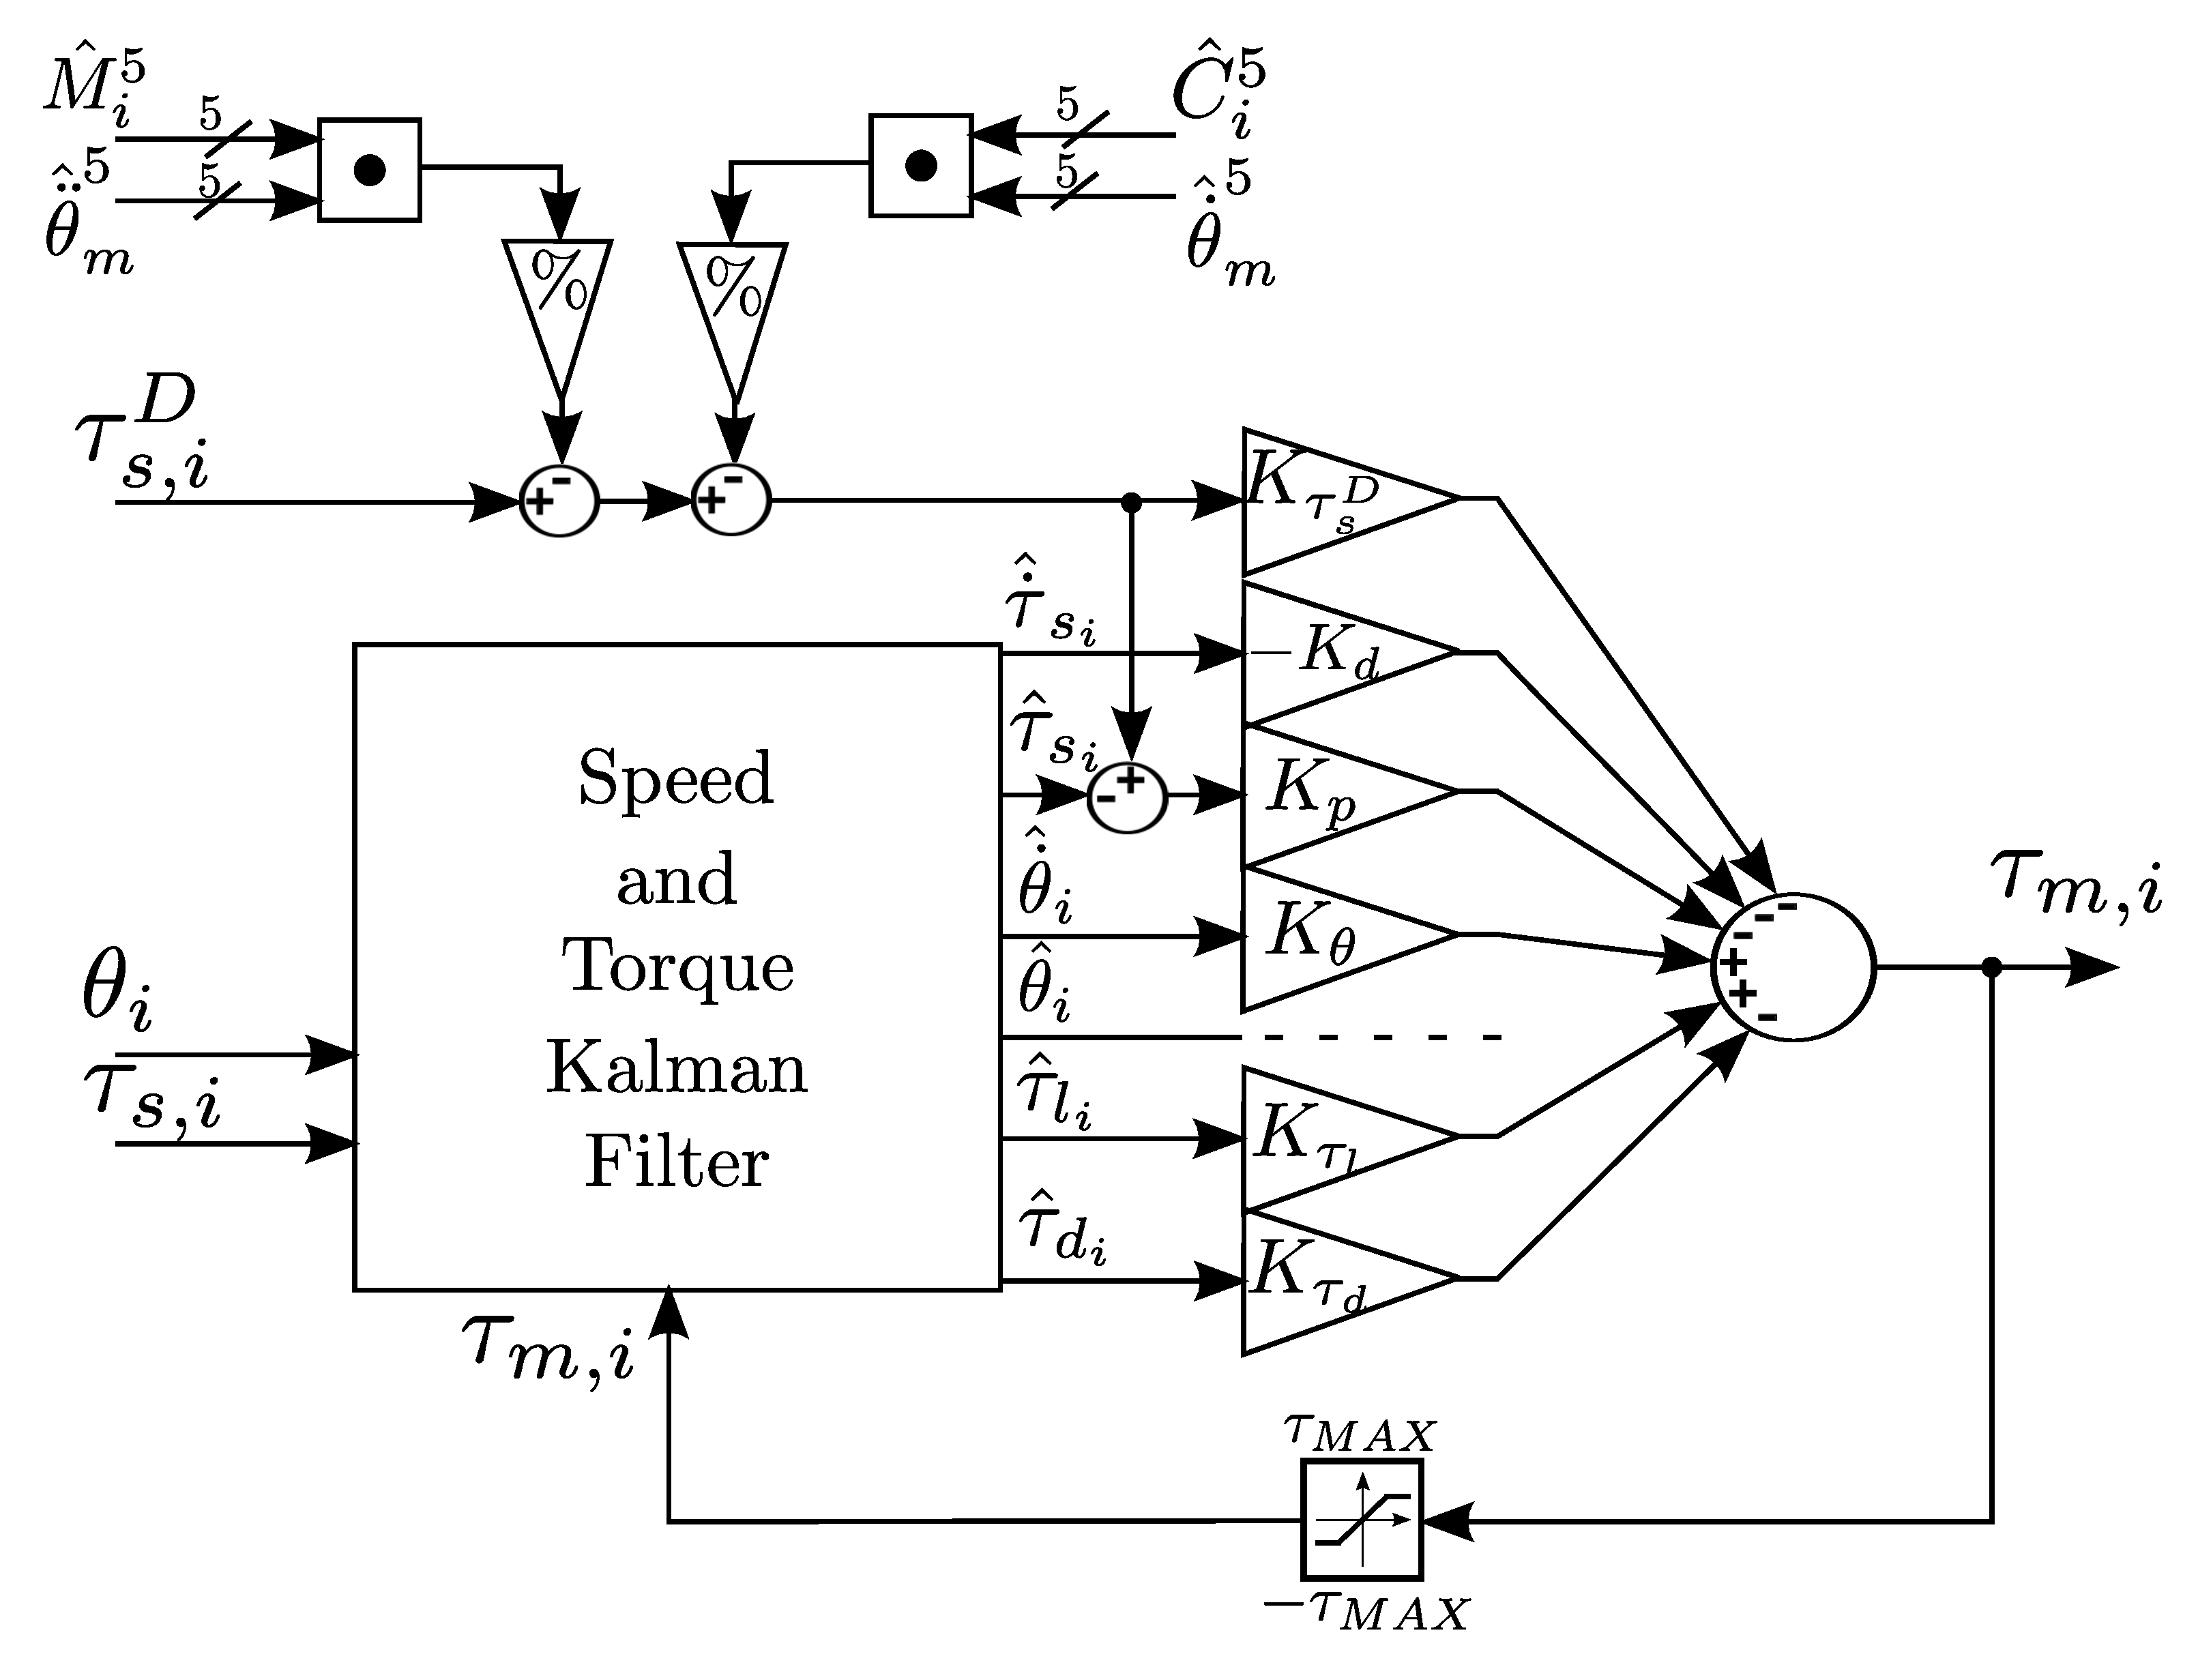
\includegraphics[width=1.0\columnwidth]{FullStateControlFeedback.pdf}
		\caption{The schema of the full state control feedback with the dynamic compensation.}
		\label{fig:full state}
	\end{figure}
	%\subsubsection{Torque tracking}
	%
	%\hl{Queste 3 formule} sono già state scritte precedentemente. ATTENZIONE! Scegli dove metterle!
	%
	%\setlength{\arraycolsep}{0.0em}
	%\begin{equation}
	%\vects{u_g} = \vects{G}(\vects{D\hat{\theta}_m})
	%\label{eq:JTCF1_control_law_a2}
	%\end{equation}
	%\begin{eqnarray}
	%\label{eq:JTCF1_control_law_b2}
	%\vects{u_f} = && - \vects{J_m} \vects{K_t}^{-1} \vects{\ddot{\tau}_s^D} + \vects{B_m} \vects{D \dot{\theta}_m} + \vects{J_m} \vects{\overline{M}^{-1}}  \vects{J^T} \vects{\hat{F}_l}  \nonumber \\
	%&&{-}\:\vects{\hat{\tau}_d} - {\vects{J}_i^{-1}} \vects{J_m} \vects{\tau_s^D} + \vects{K_p} \vects{e} + \vects{K_d} \vects{\dot{e}}	
	%\end{eqnarray}
	%\setlength{\arraycolsep}{5pt}
	%
	%\setlength{\arraycolsep}{0.0em}
	%\begin{eqnarray}
	%\label{eq:JTCF1_control_law_uf_simple2}
	%\vects{u_f} = &&\: \vects{B_m}   \vects{D \dot{\theta}_m} +  \vects{J_m} \vects{\overline{M}^{-1}} \vects{J^T} \vects{\hat{F}_l} - {\vects{J_i^{-1}}} \vects{J_m} \vects{\tau_s^D}  \nonumber \\
	%&&{-}\:\vects{\hat{\tau}_d} + \vects{K_p} \vects{e} + \vects{K_d} \vects{\dot{e}}
	%\end{eqnarray}
	%\setlength{\arraycolsep}{5pt}
	
	%\subsubsection{Impedance control / haptic rendering} \label{subsub:impedanceCJICF2}
	%
	%For the haptic rendering test, the control law was designed as an impedance control. As internal torque loop was used the law  (\ref{eq:JTCF1_control_law_uf_simple}), while the desired end-effector force $F_{ee}^D$ was chosen as
	%%
	%\begin{equation}
	%\label{eq:desiredVE}
	%\left \{
	%\begin{aligned}
	%& F_{ee}^D = 0, \ \ \ \quad \quad \quad \quad \quad \quad \quad \quad  x < x_d \\
	%& F_{ee}^D = \vectm{K_x} (\vects{x - x_d}) - \vectm{D_x}\vects{\dot{x}}, \quad  x \geq x_d  \\
	%\end{aligned}
	%\right .
	%\end{equation}
	%%
	%%\begin{equation}
	%%\tau^D = \vects{K_x} (\vects{x - x_d}) - \vects{D_x J \dot{\theta}} \frac{\vects{x - x_d}}{\left| \vects{x - x_d} \right|}
	%%\end{equation}
	%%
	%obtaining the equivalent torque control law
	%%
	%\setlength{\arraycolsep}{0.0em}
	%\begin{eqnarray}
	%\label{eq:JICF1_control_law}
	%\vects{u_f} = &&\: \vectm{B_m}  \vectm{D}\vects{\dot{\theta}_m} + \vectm{J_m} \vectm{\overline{M}^{-1}} \vectm{J^T} \vects{F_l} -\vects{\tau_d} \nonumber \\ 
	%&&{-}\: {\vectm{J}_i^{-1}} \vectm{J_m J^T}(\vectm{K_x} (\vects{x - x_d}) - \vectm{D_x}\vects{\dot{x}}) \nonumber \\ 
	%&&{+}\: \vectm{K_p} \vects{e} + \vectm{K_d} \vects{\dot{e}}
	%\end{eqnarray}
	%\setlength{\arraycolsep}{5pt}
	%%
	%where x is coordinate along the normal axis to the surface, $x_d$ is the wall coordinate, $K_x$ and $D_x$ are the desired stiffness and damping respectively of the simulated virtual environment.
	%In (\ref{eq:JICF1_control_law}) for the computation of $\vects{J} = \vects{J}(\vects{\bar{\theta}_l})$ and for the gravity compensation term is used $\vects{\bar{\theta}_l} = \vects{D} \vects{\theta_m}$.


%%%%%%%%%%%%%%%%%%%%%%%%%%%%%%%%%%%%%%%%%%%%%%%%%%%%%%%%%%%%%%%%%%%%%%%%%%%%%%%%%%%%%%%%%%%%%%%%%%%%%%%%%%%%%%%%%%%%
%%%%%%%%%%%%%%%%%%%%%%%%%%%%%%%%%%%%%%%%%%%%%%%%%%%%%%%%%%%%%%%%%%%%%%%%%%%%%%%%%%%%%%%%%%%%%%%%%%%%%%%%%%%%%%%%%%%%
\subsection{A basic state feedback controller (JTFC2)} \label{subsec:JTFC2}

The basic state feedback controller is derived assuming the following full model dynamics (extended the one introduced for a single joint by Hashimoto \cite{hashimoto1998experimental}), that differs from (\ref{eqn:dinamicaLinkMultiGiunto})  for the absence of external forces:

%\setlength{\arraycolsep}{0.0em}
%\begin{eqnarray}
%\label{eq:JICF1_control_law}
%\vects{u_f} = &&\: \vects{B_m}  \vects{D \dot{\theta}_m} + \vects{J_m} \vects{\overline{M}^{-1}} \vects{J^T} \vects{F_l} -\vects{\tau_d} \nonumber \\ 
%&&{-}\: {\vects{J}_i^{-1}} \vects{J_m J^T}(\vects{K_x} (\vects{x - x_d}) - \vects{D_x J \dot{\theta}} \frac{\vects{x - x_d}}{\left| \vects{x - x_d} \right|}) \nonumber \\ 
%&&{+}\: \vects{K_p} \vects{e} + \vects{K_d} \vects{\dot{e}}
%\end{eqnarray}
%\setlength{\arraycolsep}{5pt}



\begin{equation}
\left \{
\begin{IEEEeqnarraybox}[][c]{l}
\vectm{J_m}  \vectm{D} \vects{\ddot{\theta}_m} + \vectm{K_t}  ( \vectm{D} \vects{\theta_m} - \vects{\theta_j} ) = \vects{\tau_m} +\vects{\tau_d}  \\
\vectm{M}(\vects{\theta_j}) \vects{\ddot{\theta}_j} + \vectm{C}(\vects{\dot{\theta}_j}, \vects{\theta_j}) \vects{\dot{\theta}_j}  + \vectm{K_t}( \vects{\theta_j} - \vectm{D}\vects{\theta_m}) + \vects{G}(\vects{\theta_j}) = \vectm{J^T} \vects{F_h}
\label{dynamic_model_modifiedHashimoto_1}
\end{IEEEeqnarraybox}
\right . %\label{eqn:dinamicaMotoreMultiGiunto}
\end{equation}
%\label{eqn:dinamicaMotoreMultiGiunto} 
\normalsize


%\begin{equation}
%\label{dynamic_model_modifiedHashimoto_1}
%\vectm{J_m}  \vectm{D} \vects{\ddot{\theta}_m} + \vectm{K_t}  ( \vectm{D} \vects{\theta_m} - \vects{\theta_j} ) = \vects{\tau_m} +\vects{\tau_d}
%\end{equation}

%\begin{equation}
%\label{dynamic_model_modifiedHashimoto_2}
%\vectm{M}(\vects{\theta_j}) \vects{\ddot{\theta}_j} + \vectm{C}(\vects{\dot{\theta}_j}, \vects{\theta_j}) \vects{\dot{\theta}_j}  + \vectm{K_t}( \vects{\theta_j} - \vectm{D}\vects{\theta_m}) + \vects{G}(\vects{\theta_j}) = \vectm{J^T} \vects{F_h}
%\end{equation}

\begin{equation}
\label{dynamic_model_modifiedHashimoto_3}
\vects{\tau_s} = -\vectm{K_t} (\vectm{D}\vects{{\theta}_m} - \vects{\theta_j})
\end{equation}


Assuming the above full model dynamics, the input control $\vects{u}$ is designed as in (\ref{generic_control_law1}), where for $\vects{u}_g$ is used (\ref{eq:JTCF1_control_law_a}).
%\begin{equation}
%\label{generic_control_law2}
%\vects{u}  =  \vects{u_f} + \vects{u_g}
%\end{equation}
%
%For $\vects{u}_g$ is used (\ref{eq:JTCF1_control_law_a}). %\hl{oppure una stima del tipo $G(K^{-1}_t \tau_s - D \theta_m)$}. \\
%
%The basic control law used in \cite{hashimoto1998experimental} can be generalized in case of multi-joint robot and, according to the  proposed notation, it is
%
%\setlength{\arraycolsep}{0.0em}
%\begin{eqnarray}
%\label{JTFC2_uf_control_law_noSimplified}
%\vects{u_f} = &&\: -\vectm{J_m} \vectm{{K^{-1}_t}} ( - \vects{{\ddot{\tau}^D}_s} - \vectm{J^{-1}_i} \vectm{J_m} \vects{{\tau^D}_s} - \vectm{K_d}(\vects{\dot{\tau}_s} - \vects{{\dot{\tau}^D}_s}) \nonumber \\ 
%&&\: -\vectm{K_p}(\vects{\tau_s} - \vects{\tau^D_s})) 
%\end{eqnarray}
%\setlength{\arraycolsep}{5pt}

The basic control law used in \cite{hashimoto1998experimental} can be generalized in case of multi-joint robot. Thus, according to the  proposed notation, if one assumes  $\vects{e}=\vects{\tau_s}-\vects{\tau_s^D}$ as the error on sensor torque, given the desired sensor torque  $\vects{\tau_s^D}$, ans one assume moreover that $\vects{\dot{\tau}^D}=\vects{0}$ and  $\vects{\ddot{\tau}^D}=\vects{0}$, so that 
$\vects{\dot{e}}=\vects{\dot{\tau}_s}$ and  $\vects{\ddot{e}}=\vects{\ddot{\tau}_s}$, the control law can be written as

\setlength{\arraycolsep}{0.0em}
\begin{equation}
\label{JTFC2_control_law_final}
\vects{u_f} = - \vectm{J^{-1}_i} \vectm{J_m} \vects{\tau^D_s} + \vectm{J_m} \vectm{K^{-1}_t} \vectm{K_d} \vects{\dot{e}} + \vectm{J_m} \vectm{K^{-1}_t} \vectm{K_p} \vects{e} 
\end{equation}
\setlength{\arraycolsep}{5pt}

The modified dynamics with the control law  (\ref{JTFC2_control_law_final}), leads to the following error dynamics equations:

\setlength{\arraycolsep}{0.0em}
\begin{align}
\label{JTFC2_error_equation1}
\vects{\ddot{\theta}_m} &= \vectm{D^{-1}} \vects{\ddot{\theta}_l} - \vectm{D^{-1}} \vectm{K_t^{-1}} \vects{\ddot{e}}
\\
\label{JTFC2_error_equation2}
\vectm{J^T} \vects{F_l} - \vectm{K_t} \vectm{J^{-1}_m} \vects{\tau_d}& = \vects{\ddot{e}} + \vectm{K_d} \vects{\dot{e}} + (\vectm{K_p} + \vectm{J^{-1}_i} \vectm{K_t}) \vects{e}
\end{align}
\setlength{\arraycolsep}{5pt}


%\subsubsection{Torque tracking}
%
%\setlength{\arraycolsep}{0.0em}
%\begin{eqnarray}
%\label{JTFC2_control_law_noSimplified}
%\vects{u_f} = &&{-}\: \vects{J_m} \vects{K^{-1}_t} ( -\vects{\ddot{\tau}^D_s} - \vects{J^{-1}_i} \vects{J_m} \vects{\tau^D_s} - \vects{K_d} (\vects{\dot{\tau}_s} - \vects{\dot{\tau}^D_s})  \nonumber \\
%&&{-}\: \vects{K_p}(\vects{\tau_s} - \vects{\tau^D_s})) 
%\end{eqnarray}
%\setlength{\arraycolsep}{5pt}
%
%If one assume  $\vects{e}=\vects{\tau_s}-\vects{\tau_s^D}$ as the error on sensor torque, given the desired sensor torque  $\vects{\tau_s^D}$, ans one assume moreover that $\vects{\dot{\tau}^D}=\vects{0}$ and  $\vects{\ddot{\tau}^D}=\vects{0}$,
%so that 
%$\vects{\dot{e}}=\vects{\dot{\tau}_s}$ and  $\vects{\ddot{e}}=\vects{\ddot{\tau}_s}$, the (\ref{JTFC2_control_law_noSimplified}) can be rewritten as
%
%\begin{equation}
%\label{JTFC2_control_law}
%\vects{u_f} = - \vects{J^{-1}_i} \vects{J_m} \vects{\tau^D_s} + \vects{J_m} \vects{K^{-1}_t} \vects{K_d} \vects{\dot{e}} + \vects{J_m} \vects{K^{-1}_t} \vects{K_p} \vects{e}
%\end{equation}

%\subsubsection{Impedance control / haptic rendering}
%
%The impedance control law for the JTFC2 uses the same desired end-effector force as in (\ref{eq:desiredVE}) that leads to the equivalent torque control law
%%
%\setlength{\arraycolsep}{0.0em}
%\begin{eqnarray}
%\label{eq:JICF2_control_law}
%\vects{u_f} = &&{-}\: \vectm{J^{-1}_i} \vectm{J_m J^T}(\vectm{K_x} (\vects{x - x_d}) - \vectm{D_x}\vects{\dot{x}}) \nonumber \\
%&&{+}\: \vectm{J_m}  \vectm{K^{-1}_t} \vectm{K_d} \vects{\dot{e}} + \vectm{J_m} \vectm{K^{-1}_t} \vectm{K_p} \vects{e} 
%\end{eqnarray}
%\setlength{\arraycolsep}{5pt}
%%
%whit the same terms' meaning.
%%%%%%%%%%%%%%%%%%%%%%%%%%%%%%%%%%%%%%%%%%%%%%%%%%%%%%%%%%%%%%%%%%%%%%%%%%%%%%%%%%%%%%%%%%%%%%%%%%%%%%%%%%%%%%%%%%%%
%%%%%%%%%%%%%%%%%%%%%%%%%%%%%%%%%%%%%%%%%%%%%%%%%%%%%%%%%%%%%%%%%%%%%%%%%%%%%%%%%%%%%%%%%%%%%%%%%%%%%%%%%%%%%%%%%%%%
\subsection{A passivity-based feedback controller (JTFC3)} \label{subsec:JTFC3}

The passivity-based state feedback is derived assuming the following full model dynamics (introduced by Ott in \cite{kugi2008passivity}), that differs from  (\ref{eqn:dinamicaLinkMultiGiunto}) for the absence of the motor's viscous friction term:

\footnotesize
\begin{equation}
\left \{
\begin{IEEEeqnarraybox}[][c]{l}
\label{dynamic_model_modifiedKugi_1}
\vectm{J_m}  \vectm{D} \vects{\ddot{\theta}_m} + \vectm{C_t}(\vectm{D}\vects{\dot{\theta}_m} - \vects{\dot{\theta}_j}) + \vectm{K_t}(\vectm{D}\vects{\theta_m} - \vects{\theta_j}) = \vects{\tau_m}  \\
\vectm{M}(\vects{\theta_j}) \vects{\ddot{\theta}_j} {+}\: \vectm{C}(\vects{\dot{\theta}_j},\vects{\theta_j}) \vects{\dot{\theta}_j} + \vectm{C_t}(\vects{\dot{\theta}_j} - \vectm{D}\vects{\dot{\theta}_m})  {+}\: \vects{G}(\vects{\theta_j})+\\
 + \vectm{K}(\vects{\theta_j} - \vectm{D}\vects{\theta_m}) = \vectm{J^T} \vects{F_h} 
\end{IEEEeqnarraybox}
\right . %\label{eqn:dinamicaMotoreMultiGiunto}
\end{equation}
\normalsize


\setlength{\arraycolsep}{0.0em}
%\begin{equation}
%\label{dynamic_model_modifiedKugi_1}
%\vectm{J_m}  \vectm{D} \vects{\ddot{\theta}_m} + \vectm{C_t}(\vectm{D}\vects{\dot{\theta}_m} - \vects{\dot{\theta}_j}) + \vectm{K_t}(\vectm{D}\vects{\theta_m} - \vects{\theta_j}) = \vects{\tau_m} 
%\end{equation}
%\begin{eqnarray}
%\label{dynamic_model_modifiedKugi_2}
%\vectm{M}(\vects{\theta_j}) \vects{\ddot{\theta}_j} &&{+}\: \vectm{C}(\vects{\dot{\theta}_j},\vects{\theta_j}) \vects{\dot{\theta}_j} + \vectm{C_t}(\vects{\dot{\theta}_j} - \vectm{D}\vects{\dot{\theta}_m}) \nonumber \\
%&&{+}\: \vects{G}(\vects{\theta_j}) + \vectm{K}(\vects{\theta_j} - %\vectm{D}\vects{\theta_m}) = \vectm{J^T} \vects{F_h} 
%\end{eqnarray}
\begin{equation}
\label{dynamic_model_modifiedKugi_3}
\vects{\tau_s} = - \vectm{K_t} (\vectm{D} \vects{\theta_m} - \vects{\theta_j})
\end{equation}
\setlength{\arraycolsep}{5pt}
%
%In \cite{kugi2008passivity} the control law is
%
%\begin{equation}
%\label{generic_control_law3}
%\vects{u} =  \vects{u_f} + \vects{u_g}
%\end{equation}

In \cite{kugi2008passivity} the control law $\vects{u}$ is designed as in (\ref{generic_control_law1}) where $\vects{u_g}$ are the torques due to the gravity. For this work $\vects{u_g}$ is calculated as in (\ref{eq:JTCF1_control_law_a}). Whereas, the term $\vects{u_f}$ after some algebraic transformations can be written as:
%\hl{oppure una stima del tipo $\vects{G}(\vects{K^{-1}_t \tau_s} - \vects{D \theta_m})$ OPPURE la loro}, while the term $\vects{u_f}$ is given by
%
%\begin{equation}
%\label{control_law_Kugi_1}
%\vects{u_f} = - \vectm{J_m} \vectm{J^{-1}_{\theta}} \vects{\tau^D_s} - (\vectm{I} - \vectm{J_m} \vectm{J^{-1}_{\theta}})(\vects{\tau_s} + \vectm{B_m} \vectm{K^{-1}_t} \vects{\dot{\tau}_s})
%\end{equation}
%
%that can be rewritten as
\begin{equation}
\label{control_law_Kugi_2}
\vects{u_f} =  -\vects{\tau^D_s} + (\vectm{J_m} \vectm{J^{-1}_{\theta}} - \vectm{I}) \vectm{B_m} \vectm{K^{-1}_t} \vects{\dot{e}} + (\vectm{J_m} \vectm{J^{-1}_{\theta}} - \vectm{I}) \vects{e}
\end{equation}


%\begin{equation}
%\label{control_law_Kugi}
%\begin{align}
%\vects{u}_f &= \vects{J}_m \vects{J}^{-1}_{\theta} \vects{u}' + (\vects{I} - \vects{J}_m \vects{J}^{-1}_{\theta})(\vects{\tau}_s + \vects{B}_m \vects{K}^{-1}_t \vects{\dot{\tau}}_s) + \vects{K}_d(\vects{\dot{\tau}}_s - \vects{\dot{\tau}}^D_s) + \vects{K}_p(\vects{\tau}_s - \vects{\tau}^D_s) 
%\end{align}
%\end{equation}
%
%Ott explains the function of joint torque feedback like a motor inertia reducer, that brings the value of $\vects{B}$ to $\vects{B}_\theta$ (in our model $\vects{J}_m$ to $\vects{J}_i$). Using  \eqref{control_law_Kugi} the resulting system dynamics are given by
%
%\begin{equation}
%\label{dynamic_model_modifiedKugi_reducedInertia}
%\begin{align}
%\vects{J}_i \vects{\ddot{\theta}}_m + \vects{C}_t(\vects{D\dot{\theta}}_m - \vects{\dot{\theta}}_j) + \vects{K}_t(\vects{D\theta}_m - \vects{\theta}_j) &=  \vects{u}' \\
%\vects{M}(\vects{\theta}_j) \vects{\ddot{\theta}}_j + \vects{C}(\vects{\dot{\theta}}_j,\vects{\theta}_j) \vects{\dot{\theta}}_j + G(\vects{\theta}_j) + \vects{C}_t(\vects{D\dot{\theta}}_m - \vects{\dot{\theta}}_j) + \vects{K}_t(\vects{\theta}_j - \vects{D\theta}_m) &= \vects{J}^T \vects{F}_h \\
%\vects{\tau}_s &= - \vects{K}_t (\vects{D\theta}_m - \vects{\theta}_j)
%\end{align}
%\end{equation}
%
%where
%
%\begin{equation}
%\label{kugi_control_input}
%\begin{align}
%\vects{u}' &= -\vects{ \tau}^D_s
%\end{align}
%\end{equation}

The modified dynamics within the control law  (\ref{control_law_Kugi_2}), leads to the following error dynamics equations:

\setlength{\arraycolsep}{0.0em}

%%prova
%\footnotesize
\begin{equation}
\begin{IEEEeqnarraybox}[][c]{ll}
\label{JTFC3_error_equation_1}
\vects{\ddot{\theta}_m} = \vectm{D^{-1}} \vects{\ddot{\theta}_j} - \vectm{D^{-1}} \vectm{K_t^{-1}} \vects{\ddot{e}}  
\\
%\label{JTFC3_error_equation_2}
\vectm{K_t} \vectm{M^{-1}}\:(\vects{\theta_j})(-\vects{\tau^D_s} + \vectm{J^T} \vects{F_l}) = \nonumber \\
\vects{\ddot{e}} {+}\: ( \vectm{J_i^{-1}} +  \vectm{B^{-1}_m} \vectm{M^{-1}}(\vects{\theta_j}) \vectm{B_m}  + \vectm{K_d} \vectm{K_t}  \vectm{J^{-1}_i}) \vects{\dot{e}} + \nonumber \\
{+}\: ( \vectm{K_t} \vectm{J^{-1}_i} + \vectm{K_t} \vectm{M^{-1}}(\vects{\theta_j}) + \vectm{K_p} \vectm{K_t} \vectm{J^{-1}_i}) \vects{e} 
\end{IEEEeqnarraybox}
\end{equation}
\setlength{\arraycolsep}{5pt}
\normalsize

%\subsubsection{Torque tracking}
%
%\begin{equation}
%\label{control_law_Kugi_torque}
%\vects{u_f} = -\vects{J_m} \vects{J^{-1}_{\theta}} \vects{\tau^D_s} - (\vects{I} - \vects{J_m} \vects{J^{-1}_{\theta}})(\vects{\tau_s} - \vects{B_m} \vects{K^{-1}_t} \vects{\dot{\tau}_s})
%\end{equation}
%
%that can be rewritten as
%
%\begin{equation}
%\label{control_law_Kugi}
%\vects{u_f} =  -\vects{\tau^D_s} + (\vects{J_m} \vects{J^{-1}_{\theta}} - \vects{I}) \vects{B_m} \vects{K^{-1}_t} \vects{\dot{e}} + (\vects{J_m} \vects{J^{-1}_{\theta}} - \vects{I}) \vects{e}
%\end{equation}

%\subsubsection{Impedance control / haptic rendering}
%
%The impedance control law for the JTFC3 uses the same desired end-effector force as in (\ref{eq:desiredVE}) that leads to the equivalent torque control law
%%
%\setlength{\arraycolsep}{0.0em}
%\begin{eqnarray}
%\label{eq:JICF3_control_law}
%\vects{u_f} = &&{-}\: \vectm{J^T}(\vectm{K_x} (\vects{x - x_d}) - \vectm{D_x} \vects{\dot{x}}) \nonumber \\
%&&{+}\: (\vectm{J_m} \vectm{J^{-1}_{\theta}} - \vectm{I}) \vectm{B_m} \vectm{K^{-1}_t} \vects{\dot{e}} + ( \vectm{J_m} \vectm{J^{-1}_{\theta}} - \vectm{I}) \vects{e}
%\end{eqnarray}
%\setlength{\arraycolsep}{5pt}
%%
%whit the same terms' meaning.

%In (\ref{JICF2_control_law}) for the computation of $\vects{J} = \vects{J}(\vects{\bar{\theta}_l})$ and for the gravity compensation term is used:
%
%\begin{equation}
%\label{JICF2_control_law_theta_l_1}
%\vects{\bar{\theta}_{l,n+1}} = \vects{T_c} (\vects{\theta_{l,n}})
%\end{equation}
%\begin{equation}
%\label{JICF2_control_law_theta_l_2}
%\vects{T_c} (\vects{\theta_l}) = \vects{\theta_m} - \vects{K^{-1}_t} (\vects{G}(\vects{\theta_l}) - \vects{J^T}(\vects{\theta_l}) \vects{K_x} (\vects{x - x_d}))
%\end{equation}


%%%%%%%%%%%%%%%%%%%%%%%%%%%%%%%%%%%%%%%%%%%%%%%%%%%%%%%%%%%%%%%%%%%%%%%%%%%%%%%%%%%%%%%%%%%%%%%%%%%%%%%%%%%%%%%%%%%%
%%%%%%%%%%%%%%%%%%%%%%%%%%%%%%%%%%%%%%%%%%%%%%%%%%%%%%%%%%%%%%%%%%%%%%%%%%%%%%%%%%%%%%%%%%%%%%%%%%%%%%%%%%%%%%%%%%%%
\subsection{Impedance control / haptic rendering} \label{sub:impedanceCJICF}

The three torque control laws are used as inner feedback loop of the impedance control used to test the exoskeleton in the haptic rendering task. The desired end-effector force $F_{ee}^D$ is due to the interaction with the virtual environment impedance. More in detail, the desired force is defined by:
%
\begin{equation}
\label{eq:desiredVE}
\left \{
\begin{aligned}
& \vect{ F_{ee}^D} = 0, \ \ \ \quad \quad \quad \quad \quad \quad \quad \quad  x < x_d \\
& \vect{F_{ee}^D} = \vectm{K_x} (\vects{x - x_d}) - \vectm{D_x}\vects{\dot{x}}, \quad  x \geq x_d  \\
\end{aligned}
\right .
\end{equation}
%
%\begin{equation}
%\tau^D = \vects{K_x} (\vects{x - x_d}) - \vects{D_x J \dot{\theta}} \frac{\vects{x - x_d}}{\left| \vects{x - x_d} \right|}
%\end{equation}
%
%obtaining the equivalent torque control law
%%
%\setlength{\arraycolsep}{0.0em}
%\begin{eqnarray}
%\label{eq:JICF1_control_law}
%\vects{u_f} = &&\: \vectm{B_m}  \vectm{D}\vects{\dot{\theta}_m} + \vectm{J_m} \vectm{\overline{M}^{-1}} \vectm{J^T} \vects{F_l} -\vects{\tau_d} \nonumber \\ 
%&&{-}\: {\vectm{J}_i^{-1}} \vectm{J_m J^T}(\vectm{K_x} (\vects{x - x_d}) - \vectm{D_x}\vects{\dot{x}}) \nonumber \\ 
%&&{+}\: \vectm{K_p} \vects{e} + \vectm{K_d} \vects{\dot{e}}
%\end{eqnarray}
%\setlength{\arraycolsep}{5pt}
%
where $\vect{x}$ is the coordinate along the normal axis to the surface, $\vect{x_d}$   is the wall coordinate, $\vectm{K_x}$ and $\vectm{D_x}$ are the desired stiffness and damping respectively of the simulated virtual environment.

%%%%%%%%%%%%%%%%%%%%%%%%%%%%%%%%%%%%%%%%%%%%%%%%%%%%%%%%%%%%%%%%%%%%%%%%%%%%%%%%%%%%%%%%%%%%%%%%%%%%%%%%%%%%%%%%%%%%
%%%%%%%%%%%%%%%%%%%%%%%%%%%%%%%%%%%%%%%%%%%%%%%%%%%%%%%%%%%%%%%%%%%%%%%%%%%%%%%%%%%%%%%%%%%%%%%%%%%%%%%%%%%%%%%%%%%%


%%%%%%%%%%%%%%%%%%%%%%%%%%%%%%%%%%%%%%%%%%%%%%%%%%%%%%%%%%%%%%%%%%%%%%%%%%%%%%%%%%%%%%%%%%%%%%%%%%%%%%%%%%%%%%%%%%%%
%%%%%%%%%%%%%%%%%%%%%%%%%%%%%%%%%%%%%%%%%%%%%%%%%%%%%%%%%%%%%%%%%%%%%%%%%%%%%%%%%%%%%%%%%%%%%%%%%%%%%%%%%%%%%%%%%%%%
%%%%%%%%%%%%%%%%%%%%%%%%%%%%%%%%%%%%%%%%%%%%%%%%%%%%%%%%%%%%%%%%%%%%%%%%%%%%%%%%%%%%%%%%%%%%%%%%%%%%%%%%%%%%%%%%%%%%
%%%%%%%%%%%%%%%%%%%%%%%%%%%%%%%%%%%%%%%%%%%%%%%%%%%%%%%%%%%%%%%%%%%%%%%%%%%%%%%%%%%%%%%%%%%%%%%%%%%%%%%%%%%%%%%%%%%%

%DIFDELCMD < 
\section{Experiments and Results} \label{sec:experimentsResults}

The performance of the torque and impedance controls have been assessed by experimental tests. 
The tests show how the torque controls behave in constant and varying desired torque tracking.
The first one is the transparency test in which the robot tries to keep the joint torque at zero Nm while the user is moving the exoskeleton.
The second test is the haptic rendering with a slanted flat surface with different simulated stiffness.
More details on each test are reported in the subsections below.
\par The implemented control laws (\ref{eq:JTCF1_control_law_uf_simple}), (\ref{JTFC2_control_law_final}) and (\ref{control_law_Kugi_2}) have been set using the model parameters. The proportional and derivative PD gains ($K_p$ and $K_d$) have been chosen to obtain a desired error dynamics, more in detail the form that guarantees the minimum ITAE index. Notice that the control laws (\ref{eq:JTCF1_control_law_uf_simple}) and (\ref{JTFC2_control_law_final}) have two degrees of freedom, i.e. $K_p$ and $K_d$ can be independently chosen, whereas the control law (\ref{control_law_Kugi_2}) exhibits a 1 degree of freedom, thus the two control gains are linked and they are calculated as a function of the desired inertia $J_{\theta}$.

%%%%%%%%%%%%%%%%%%%%%%%%%%%%%%%%%%%%%%%%%%%%%%%%%%%%%%%%%%%%%%%%%%%%%%%%%%%%%%%%%%%%%%%%%%%%%%%%%%%%%%%%%%%%%%%%%%%%
%%%%%%%%%%%%%%%%%%%%%%%%%%%%%%%%%%%%%%%%%%%%%%%%%%%%%%%%%%%%%%%%%%%%%%%%%%%%%%%%%%%%%%%%%%%%%%%%%%%%%%%%%%%%%%%%%%%%
\subsection{Transparency} \label{subsec:transparency}

For the transparency test, two kinds of trials have been done.
The first type of trial uses the JTFC1 control law described in the subsection \ref{subsec:JTFC1} in order to verify how much the dynamics compensations improve the desired torque tracking.
The second type of trials are useful to compare the three control laws and to understand how the terms of the control inputs are related to the desired torque tracking.
During the transparency tests the user has been linked with the exoskeleton in 2 points: the arm in order to transmit the shoulder movement, and the forearm in order to exchange the elbow movement.
\par In order to validate the interaction torque control and to evaluate the torque tracking performance, an additional force sensor has been mounted on the end-effector of the exoskeleton to measure the actual forces $\vects{F_h^*}$  applied by the user. 
As transparency index the measured end effector norm force and the reflected torques at the joints have been used.
The reflected torques at the joint are calculated as $\vects{\tau_s^*}=\vects{J^T F_h^*}$ and then compared to the interaction torques estimated by the optimal observer.

\subsubsection{How dynamic compensation affects the transparency} \label{subsubsec:compensationAndTransparency}

In order to understand how the dynamic compensation affects the transparency the scheme of figure \ref{fig:full state} has been implemented, that uses the JTFC1 control law plus the dynamics terms multiplied by $\alpha$, with $0 \leq \alpha \leq 1$.

The experimental results for torque tracking, with a desired torque $\vects{\tau_s^D=0}$, are shown for the second joint $J_2$ in \figurename \ \ref{fig:torque_validation}, that is the joint with the highest link inertia. A user has moved without constraints the exoskeleton, grabbing the force sensor mounted at the end effector. The control was set to follow his movement at zero-torque without (\figurename \ \ref{fig:torque_validation_nocomp}) and with (\figurename \ \ref{fig:torque_validation_comp}) dynamics compensation. 
\par The upper plots show the joint position (blue solid line) and acceleration (red dotted line), to demonstrate the movements were similar in both cases. The lower plots represent the interaction torques estimated by the observer (blue solid line) and measured by the force sensor (red dotted line). Even if the estimated torques are similar in both cases, with dynamics compensation the actual interaction forces are lower, demonstrating that torque tracking is more precise and the user has to compensate less for the links dynamics.

\begin{figure}[htb]
	\centering
	\subfigure[Without dynamics compensation]{ 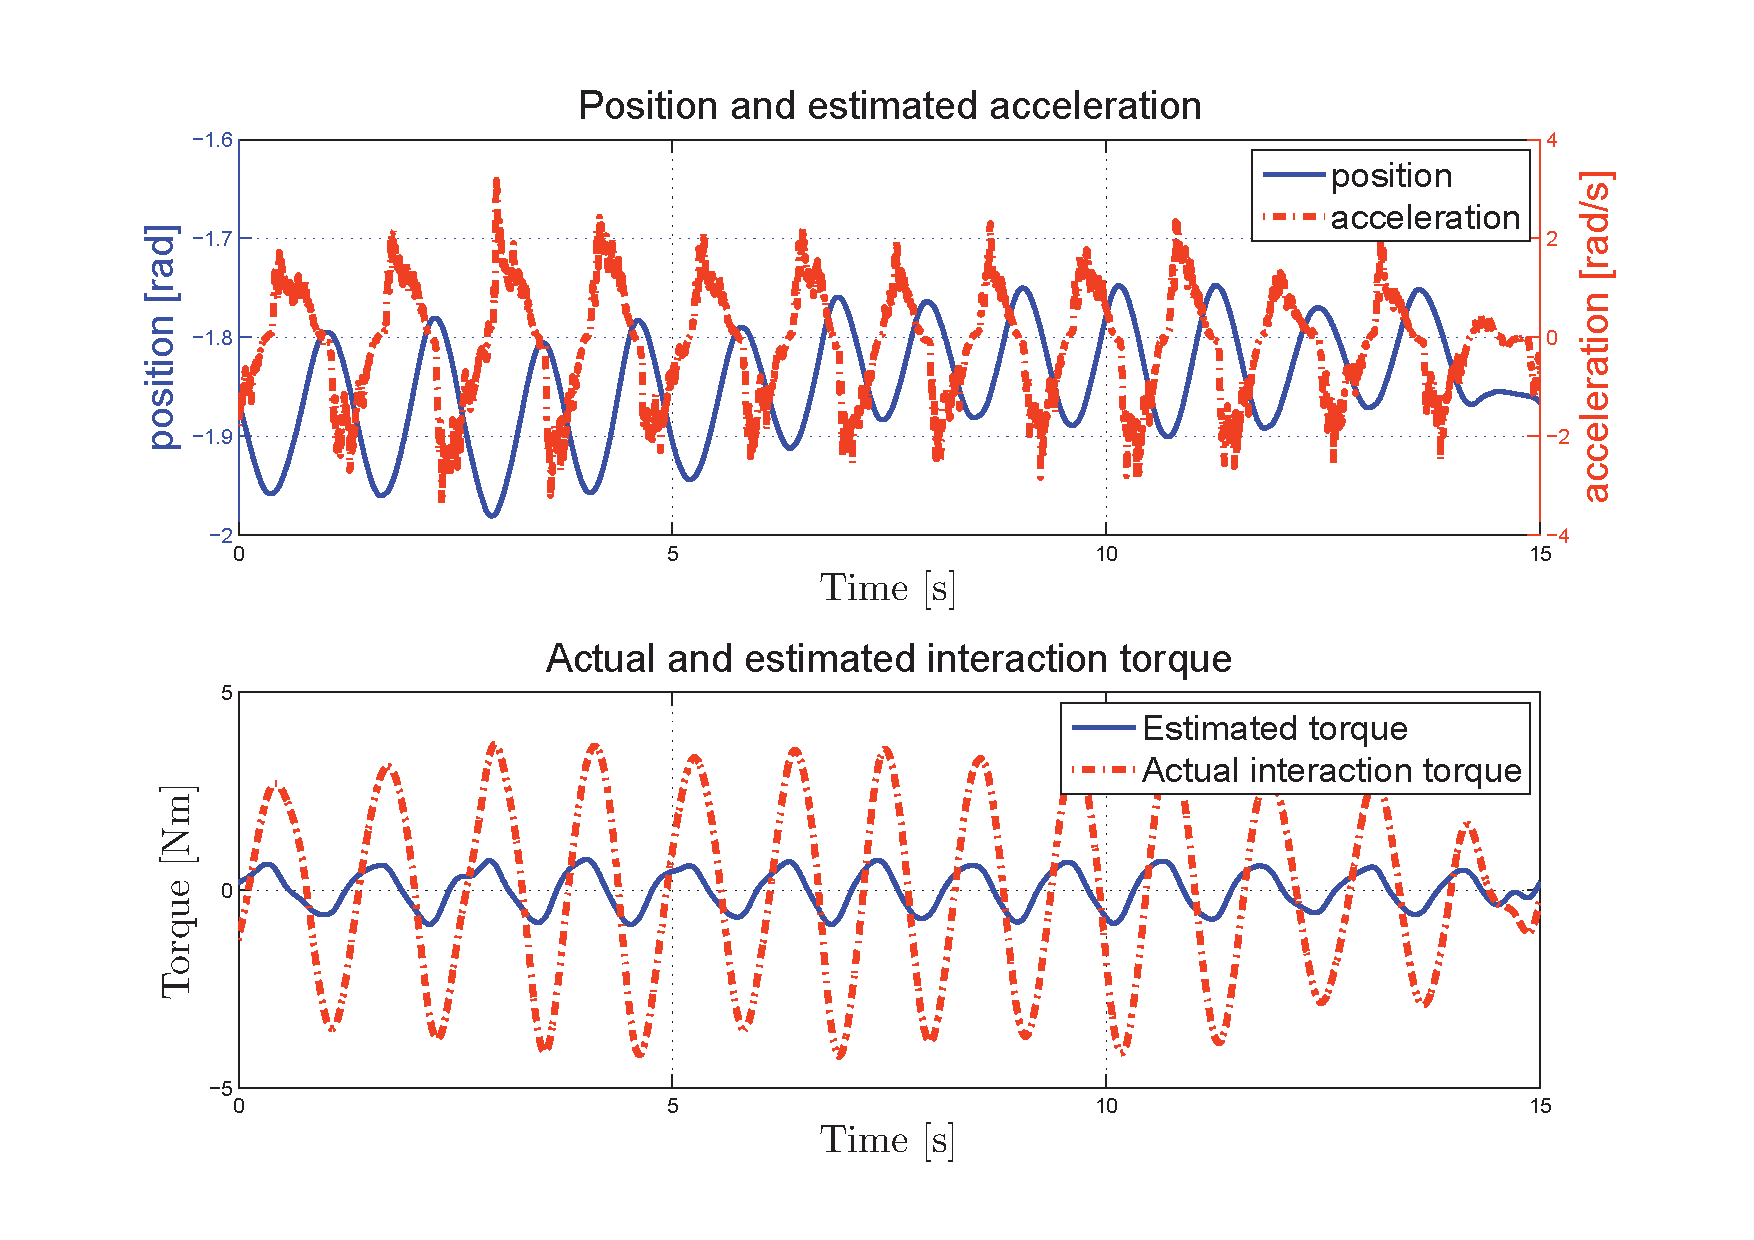
\includegraphics[width=1\columnwidth]{a_p_ts2_vs_ets2_nocomp.pdf}\label{fig:torque_validation_nocomp}}
	\subfigure[With dynamics compensation]{  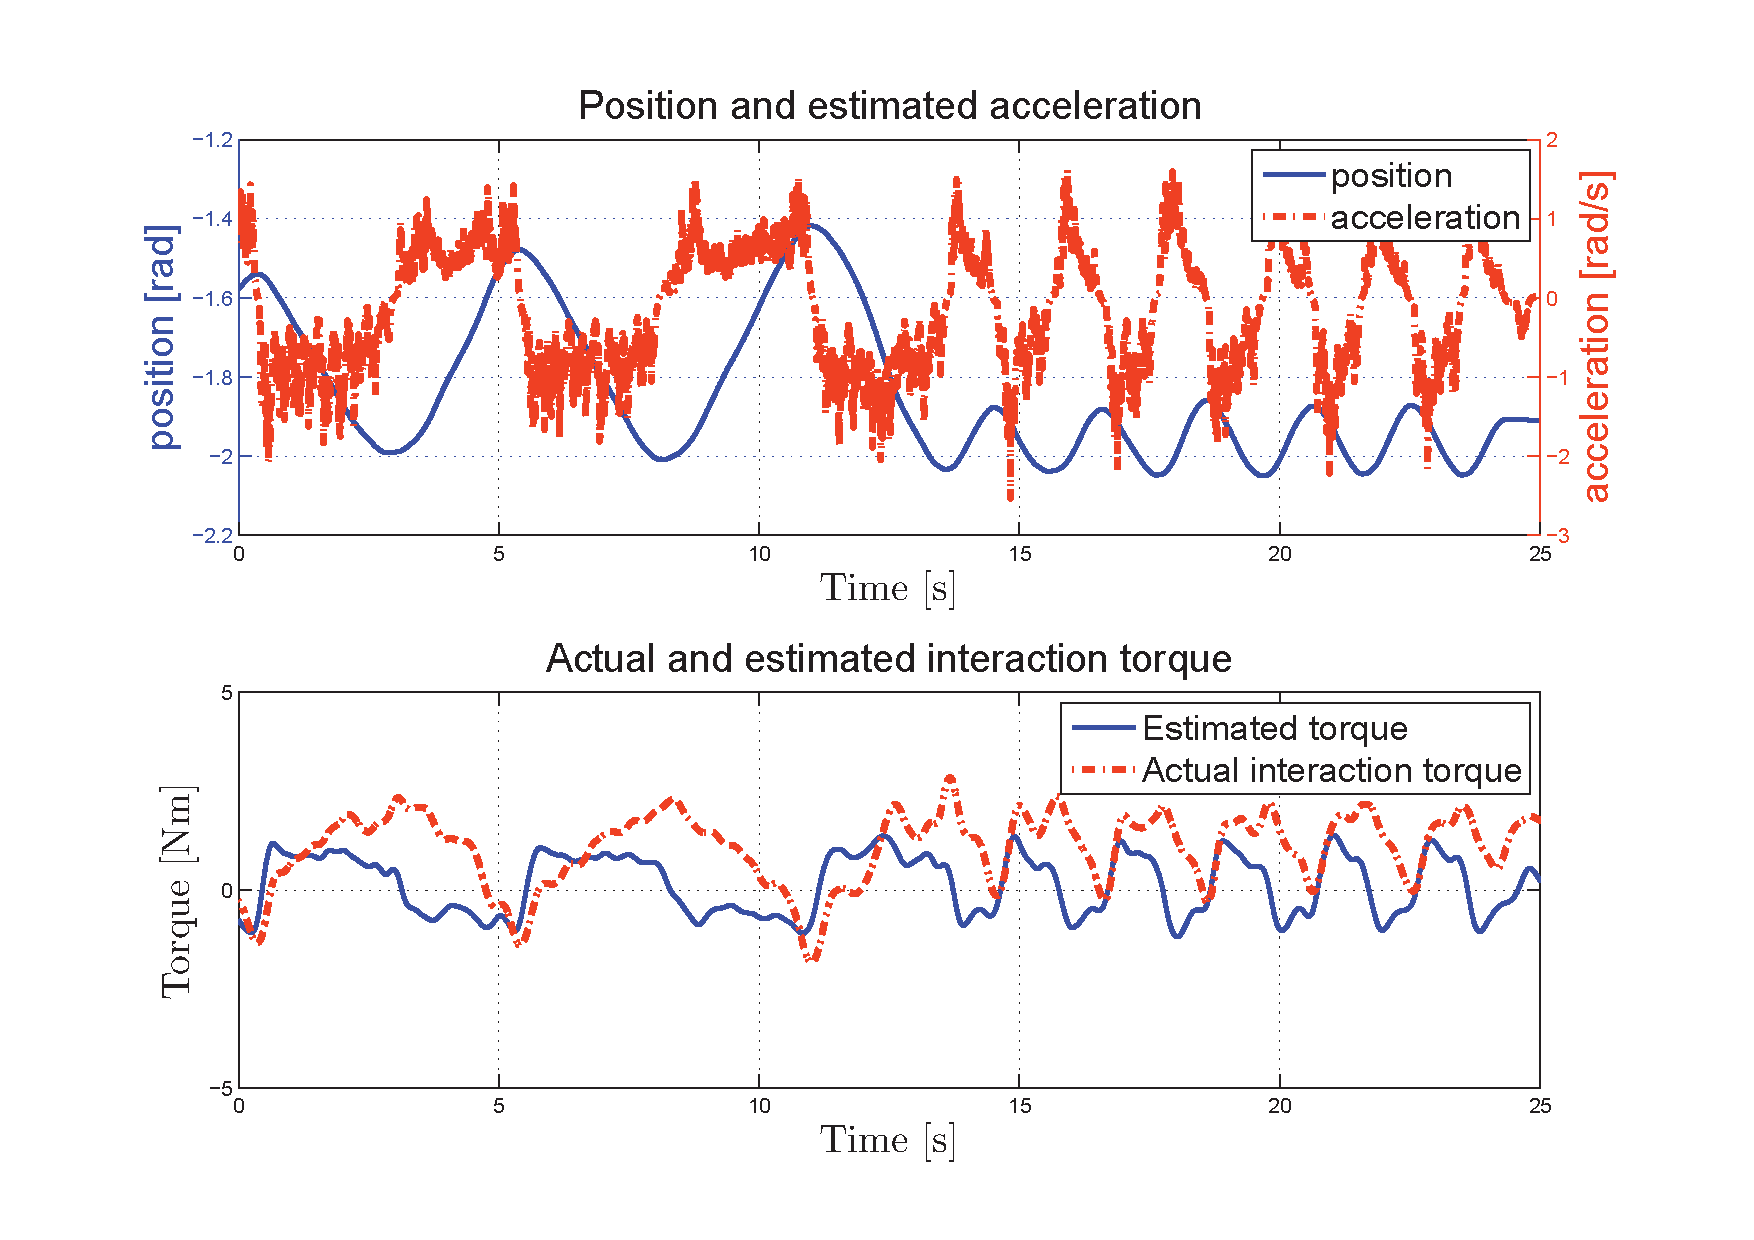
\includegraphics[width=1\columnwidth]{a_p_ts2_vs_ets2_comp.pdf}\label{fig:torque_validation_comp}}
	\caption{Comparison between the measured torque $\tau_s$ and calculated torque by force sensor}
	\label{fig:torque_validation}
\end{figure}



\subsubsection{Comparison between the three torque controllers JTFC1, JTFC2 and JTFC3}
For this kind of trials the three joint torque controls presented in the section \ref{sec:Full_state_feedback_controllers} were tested with a desired torque set to zero ($\vects{\tau_s^D=0}$) as for the trials in the subsection \ref{subsubsec:compensationAndTransparency}. 
\par In order to have comparable results and repeatability of trials, the transparency of the exoskeleton was tested with the same subject while he was trying to perform the same circular trajectory at the end effector, with the same velocity using the three different controls. The subject had visual cue (a circle of 150 mm of radius) while performing the task.
To evaluate the transparency performances only data in the same range of speed were used.
Despite the user tried to track the desired trajectory, the executed ones and their speeds were someway influenced by the used torque control. The average speed at the end effector of the three controls are listed in the \tablename \ \ref{tab:transparencySpeeds}.
%
%\begin{table}[!t]
%	\renewcommand{\arraystretch}{1.3}
%	\caption{The natural frequency of the joints}
%	\label{tab:transparencySpeeds}
%	\centering
%	\begin{tabular}{|c|c|c|}
%		\hline
%		\bfseries Control & \bfseries Avg. speed [$m/s$] & \bfseries Std. dev. [$m/s$]\\
%		\hline\hline
%		JTFC1 & 0.4198 & 0.0810\\
%		\hline
%		JTFC2 & 0.4460 & 0.1374\\
%		\hline
%		JTFC3 & 0.3867 & 0.1213\\
%		\hline
%	\end{tabular}
%\end{table}
\begin{table}[]
	\renewcommand{\arraystretch}{1.3}
	\caption{Mean and Std. Dev. of the e.e. speed in the transparency experiments}
	\label{tab:transparencySpeeds}
	\centering
	\begin{tabular}{c c c}
		\hline \hline
		\bfseries Control & \bfseries Avg. speed [$m/s$] & \bfseries Std. dev. [$m/s$]\\
		\hline
		JTFC1 & 0.4198 & 0.0810\\
		JTFC2 & 0.4460 & 0.1374\\
		JTFC3 & 0.3867 & 0.1213\\
		\hline \hline
	\end{tabular}
\end{table}
%
The real trajectories can be shown in the \figurename \ \ref{fig:traittorie3D}.
\begin{figure}[htb]
	\centering
	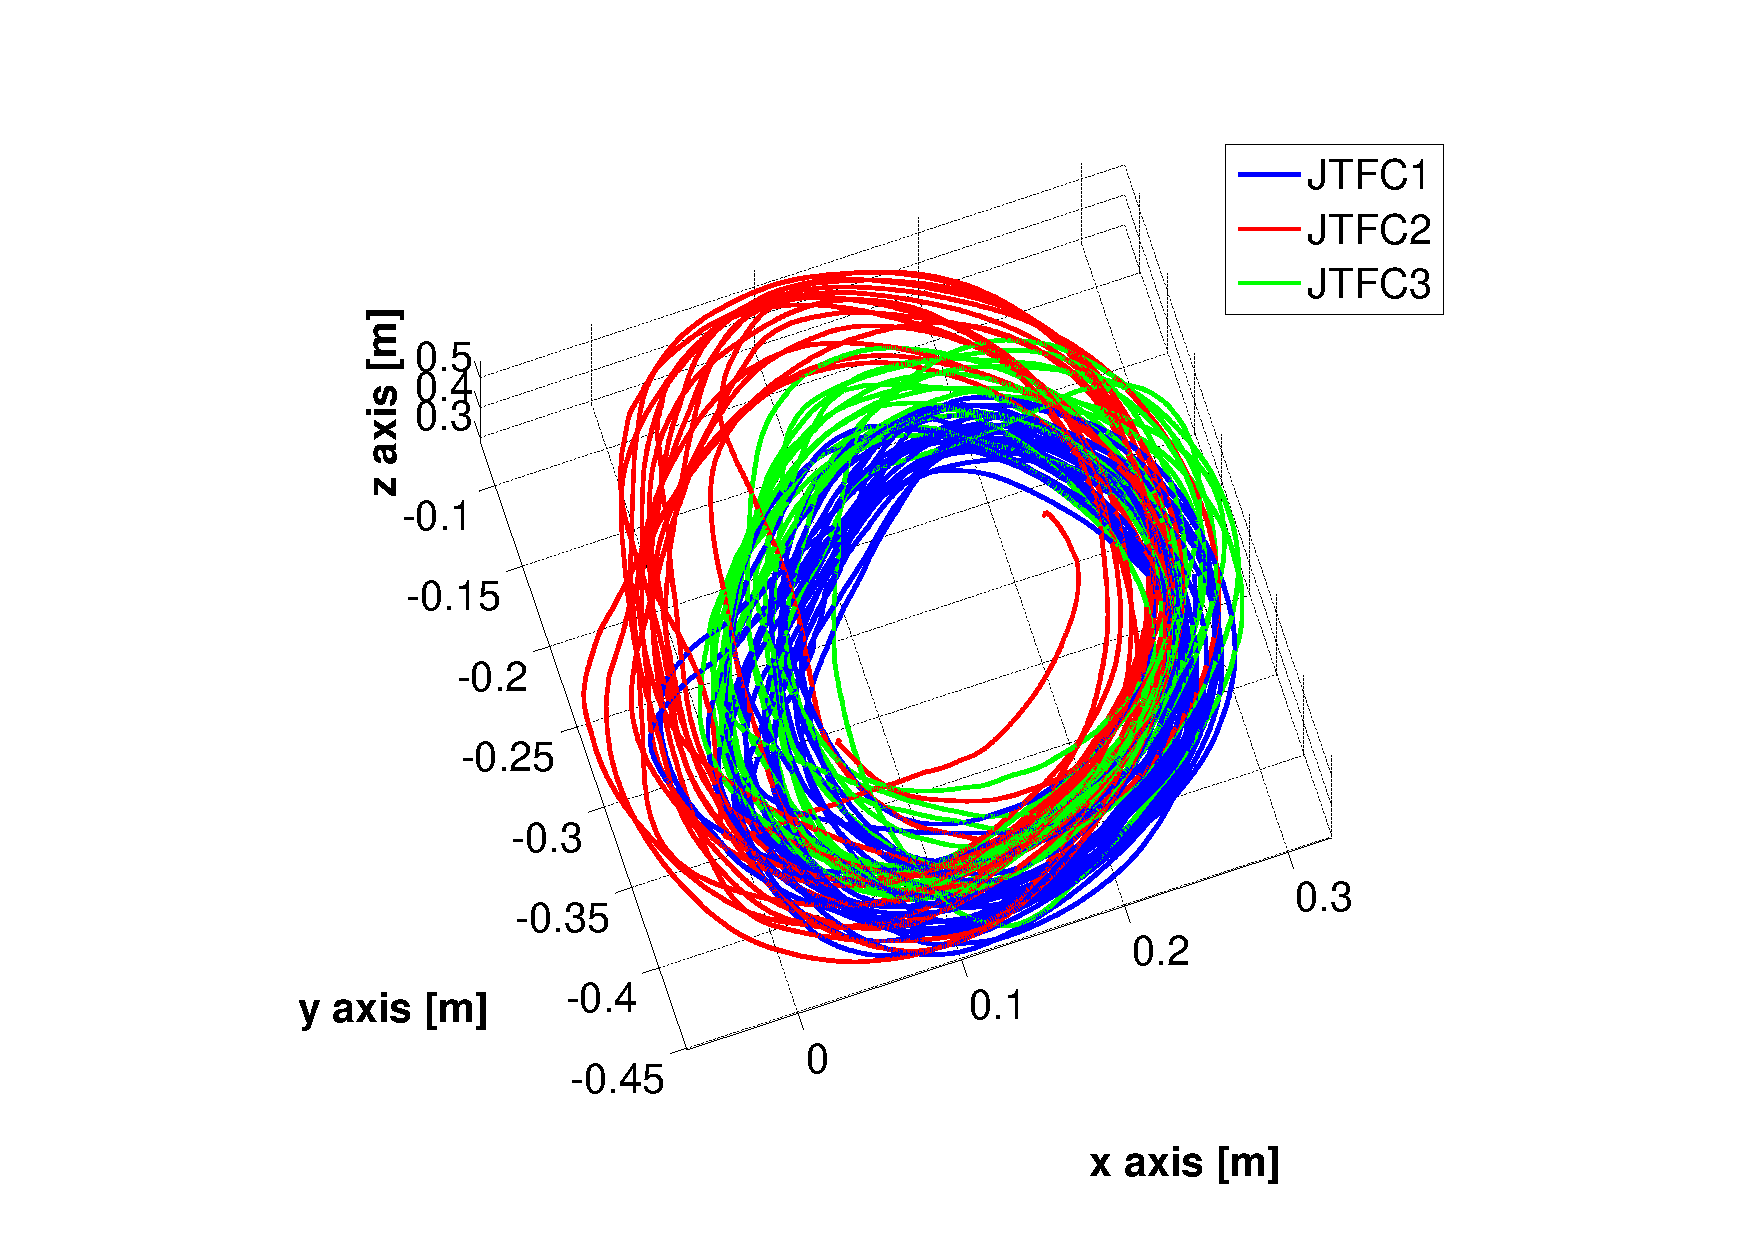
\includegraphics[width=0.99\columnwidth]{traiettorieCircolari2}
	\caption{The trajectories performed during the transparency test using the three control laws.}
	\label{fig:traittorie3D}
\end{figure}
%\begin{figure}[htb]	
%	\centering
%	\includegraphics[width=0.7\columnwidth]{\figpath{traiettorieCircolariPianoXY}}
%	\label{fig:traiettorieXY}
%	\caption{The Rehab-Exos CAD model showing overall kinematics and actuator structure}
%\end{figure}
%
\par As the reader can see, the red trajectories (the ones obtained by using the control JTFC2) are less accurate due to the limited torque control performance. Moreover, from the analysis of the control torque errors at the joints (\figurename \ \ref{fig:transparencyJointErrors}), it can be seen that the control JTFC2 exhibits an average error that is independent from the link inertia. The torque error over link inertia ratio for the elbow joint is the highest and this leads to a greater disturbance on the fine trajectory execution.
\begin{figure}[htb]
	\centering
	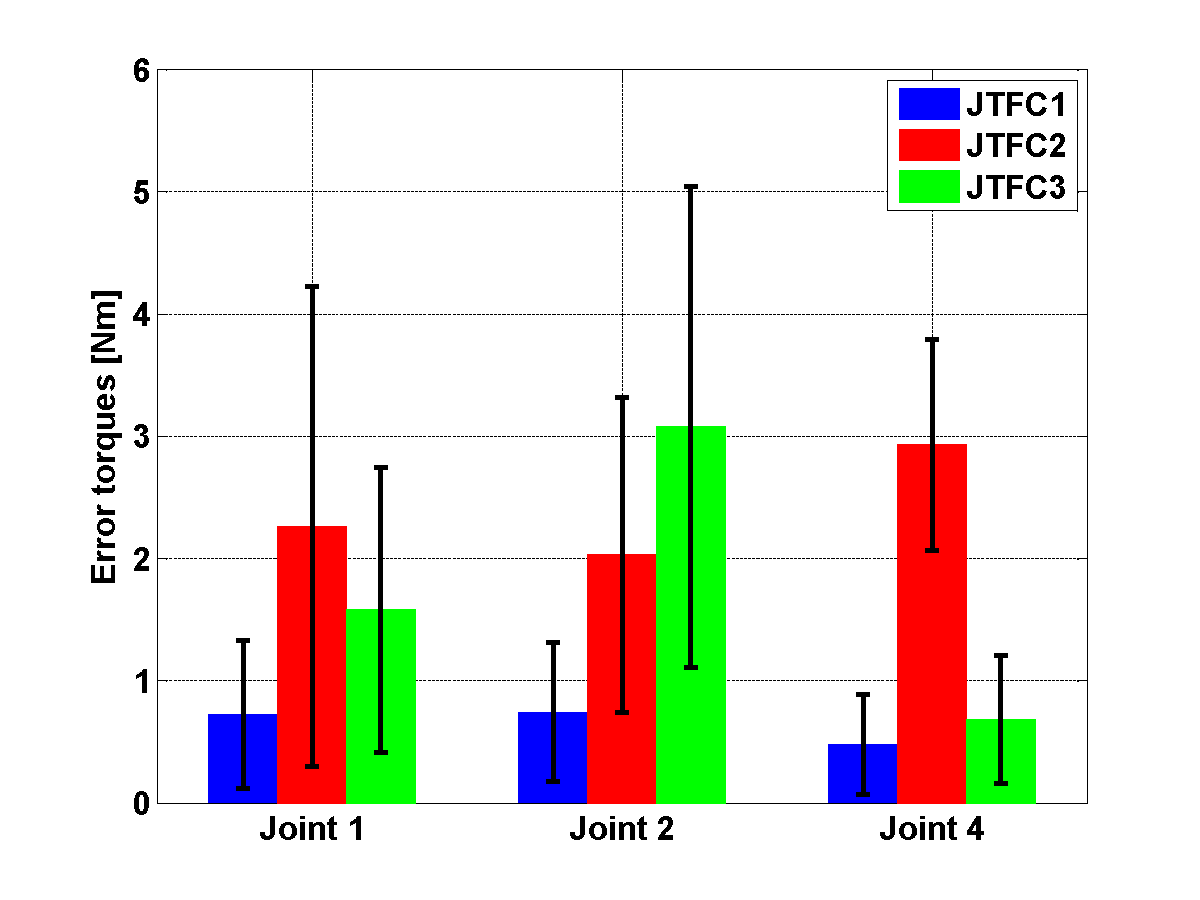
\includegraphics[width=1\columnwidth]{erroriTrasparenzaGiunti}
	\caption{The torque errors of the 3 controllers for joints 1, 2 and 4.}
	\label{fig:transparencyJointErrors}
\end{figure}
%
The average force measured at the end effector are shown in \figurename \ \ref{fig:transparencyEeErrors}.
\begin{figure}[htb]
	\centering
	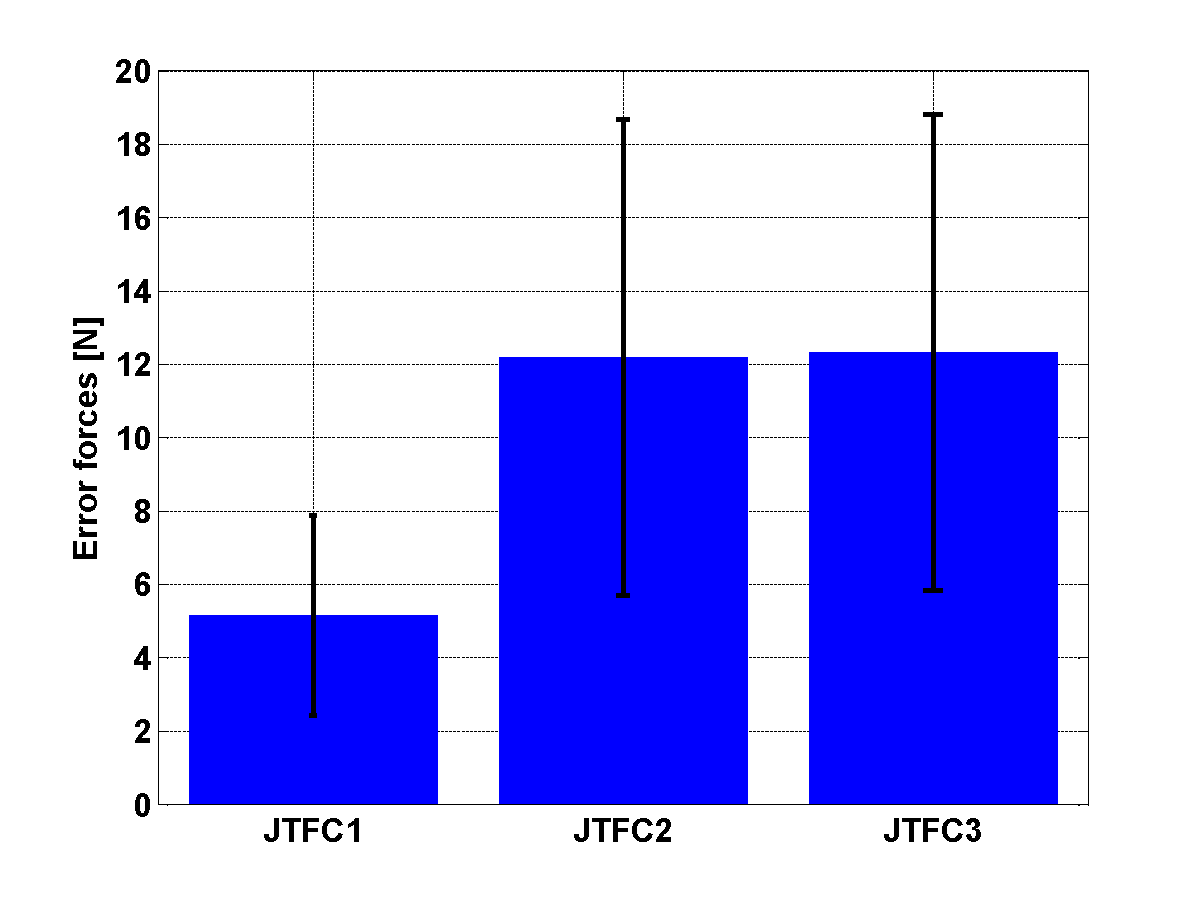
\includegraphics[width=1\columnwidth]{erroreForzaEETrasparenza}
	\caption{The force error at the end effector of the 3 controllers.}
	\label{fig:transparencyEeErrors}
\end{figure}
%
\par The value of the end-effector forces provides an overall index of the exoskeleton transparency with a given torque control (when $\vects{\tau_s^D=0}$). The control JTFC1 that implements a full-state feedback control performs better because it models in a more accurate and general way the joint dynamics. Moreover, the control JTFC1 compensates for the modeled effects. Notice that, at joint level, the control JTFC3 behaves more similar to JTFC1 rather than to the control JTFC2, in fact the torque errors of the control JTFC1 and JTFC3 seems to be correlated to the link inertia.

%%%%%%%%%%%%%%%%%%%%%%%%%%%%%%%%%%%%%%%%%%%%%%%%%%%%%%%%%%%%%%%%%%%%%%%%%%%%%%%%%%%%%%%%%%%%%%%%%%%%%%%%%%%%%%%%%%%%
%%%%%%%%%%%%%%%%%%%%%%%%%%%%%%%%%%%%%%%%%%%%%%%%%%%%%%%%%%%%%%%%%%%%%%%%%%%%%%%%%%%%%%%%%%%%%%%%%%%%%%%%%%%%%%%%%%%%
\subsection{Haptic rendering}

The implemented torque controls can be used to render the interaction forces exchanged with a virtual surface of a given stiffness and damping, acting as impedance controls. In these tests the contact forces at the end-effector are proportional to the penetration length of the end-effector into the virtual wall surface and to its speed. The force is then converted to desired torques at the joints by multiplying the equation defined in (\ref{eq:desiredVE}) by the transpose of the Jacobian, where the equations (\ref{eq:JTCF1_control_law_uf_simple}), (\ref{JTFC2_control_law_final}) and (\ref{control_law_Kugi_2}) have been used respectively for JFTC1, JFTC2 and JFTC3.
%The design of the exoskeleton allows to control the torque on every joint, so it is possible to render an interaction force not only at the end effector but on every link of the robot. In this case, in equation (\ref{jacobian}) a modified Jacobian will be used to convert forces not applied on the end effector.
\par In the experiments the user grabs the exoskeleton only at the end effector without applying any other force on the links. In this way, the forces measured by the end-effector's force sensor have been used to evaluate the overall system performance since these forces are not involved for the torque control.
\par The rendering experiments were composed by four different type of trials as depicted in \figurename \ \ref{fig:renderingTestType}:
\begin{itemize}
	\item T1: "Slide on surface" experiment with moderate forces;
	\item T2: "Slide on surface" experiment with high forces;
	\item T3: "Collision with a surface" experiment with moderate speed;
	\item T4: "Collision with a surface" experiment with high speed.
\end{itemize}

During the T1 and T2 trials the experimenter slided the end-effector on the surface without sudden variations of penetration. The difference between the T1 and T2 trials is the average level of force along the orthogonal axes at the surface.
In the T3 and T4 trials the aim is to test the dynamic performance of the controls, so the experimenter pushed the end-effector on the surface. The difference between the T3 and T4 trials is the average slope of the desired force profiles.
The 4 tests have been evaluated for each controls and with three different environment parameters, in order to consider a low, an intermediate and a high stiff wall. 
\begin{figure}[htb]
	\centering
	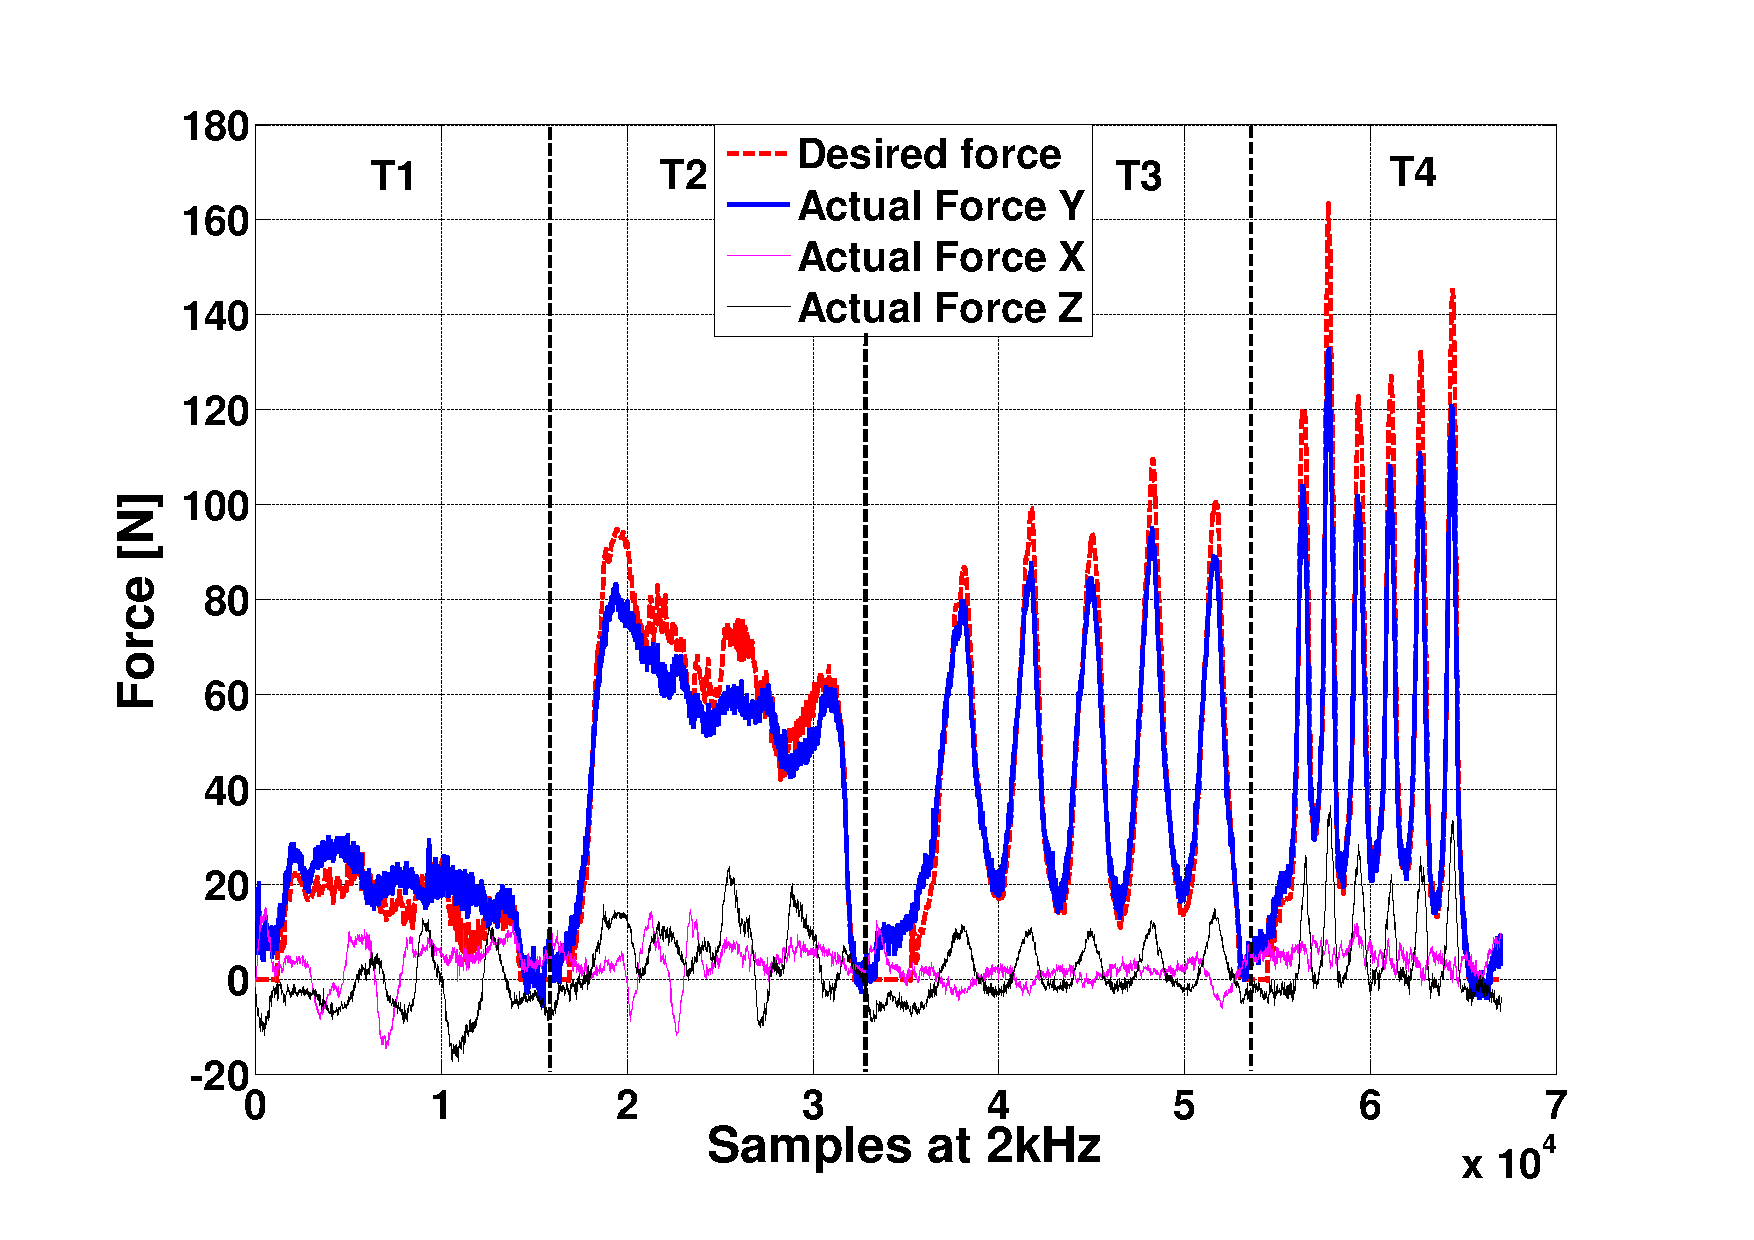
\includegraphics[width=1\columnwidth]{proveRendering}
	\caption{The four trial types during an haptic rendering test. The desired forces is plotted with red dashed lines, the measured orthogonal forces are plotted with blue solid lines while the two tangential components are with magenta and black solid lines.}
	\label{fig:renderingTestType}
\end{figure}

\par The \tablename \ \ref{tab:meanForcesRendering} reports the three environment parameters, the average forces involved in the T1 and T2 trials, the average force peaks and the average slope of the T3 and T4 trials.
%\begin{table}[!t]
%	\renewcommand{\arraystretch}{1.3}
%	\caption{The average forces involved in the T1 and T2 trials, the average force peaks and the average slope of the T3 and T4 trials.}
%	\label{tab:meanForcesRendering}
%	\centering
%	\begin{tabular}{|c|c|c|c|c|}
%		\hline
%		\bfseries Env. Params. & \bfseries T1 & \bfseries T2 & \bfseries T3 & \bfseries T4 \\
%		\hline\hline
%		5 kN/m  &  22.22 $N$ & 50.79 $N$ & 83.33 $N$ & 112.33 $N$\\ 2 Ns/m & - & - & 127.28 $N/s$ & 518.49 $N/s$\\ 
%		\hline
%		20 kN/m &  22.81 $N$ & 66.14 $N$ & 103.97 $N$ & 136.97 $N$\\ 7 Ns/m & - & - & 159.25 $N/s$ & 550.99 $N/s$\\
%		\hline
%		40 kN/m  &  24.98 $N$ & 59.37 $N$ & 88.32 $N$ & 126.20 $N$\\ 10 Ns/m & - & - & 120.39 $N/s$ & 616.03 $N/s$\\
%		\hline
%	\end{tabular}
%\end{table}
\begin{table}[]
	\renewcommand{\arraystretch}{1.3}
	\caption{The average forces involved in the T1 and T2 trials, the average force peaks and the average slope of the T3 and T4 trials.}
	\label{tab:meanForcesRendering}
	\centering
	\begin{tabular}{c c c c c}
		\hline \hline
		\bfseries Env. Params. & \bfseries T1 & \bfseries T2 & \bfseries T3 & \bfseries T4 \\
		\hline
		5 kN/m  &  22.22 $N$ & 50.79 $N$ & 83.33 $N$ & 112.33 $N$\\ 2 Ns/m & - & - & 127.28 $N/s$ & 518.49 $N/s$\\ 
		\hline
		20 kN/m &  22.81 $N$ & 66.14 $N$ & 103.97 $N$ & 136.97 $N$\\ 7 Ns/m & - & - & 159.25 $N/s$ & 550.99 $N/s$\\
		\hline
		40 kN/m  &  24.98 $N$ & 59.37 $N$ & 88.32 $N$ & 126.20 $N$\\ 10 Ns/m & - & - & 120.39 $N/s$ & 616.03 $N/s$\\
		\hline \hline
	\end{tabular}
\end{table}

\par To evaluate the performances of the three different torque controls three indexes have been proposed, i.e. 
\begin{itemize}
	\item the mean of the norm of the error force vectors;
	\item the mean of the absolute value of the error of the orthogonal component;
	\item the mean of the angle between the desired forces and the measured ones.
\end{itemize}

\begin{figure}[htb]
	\centering
	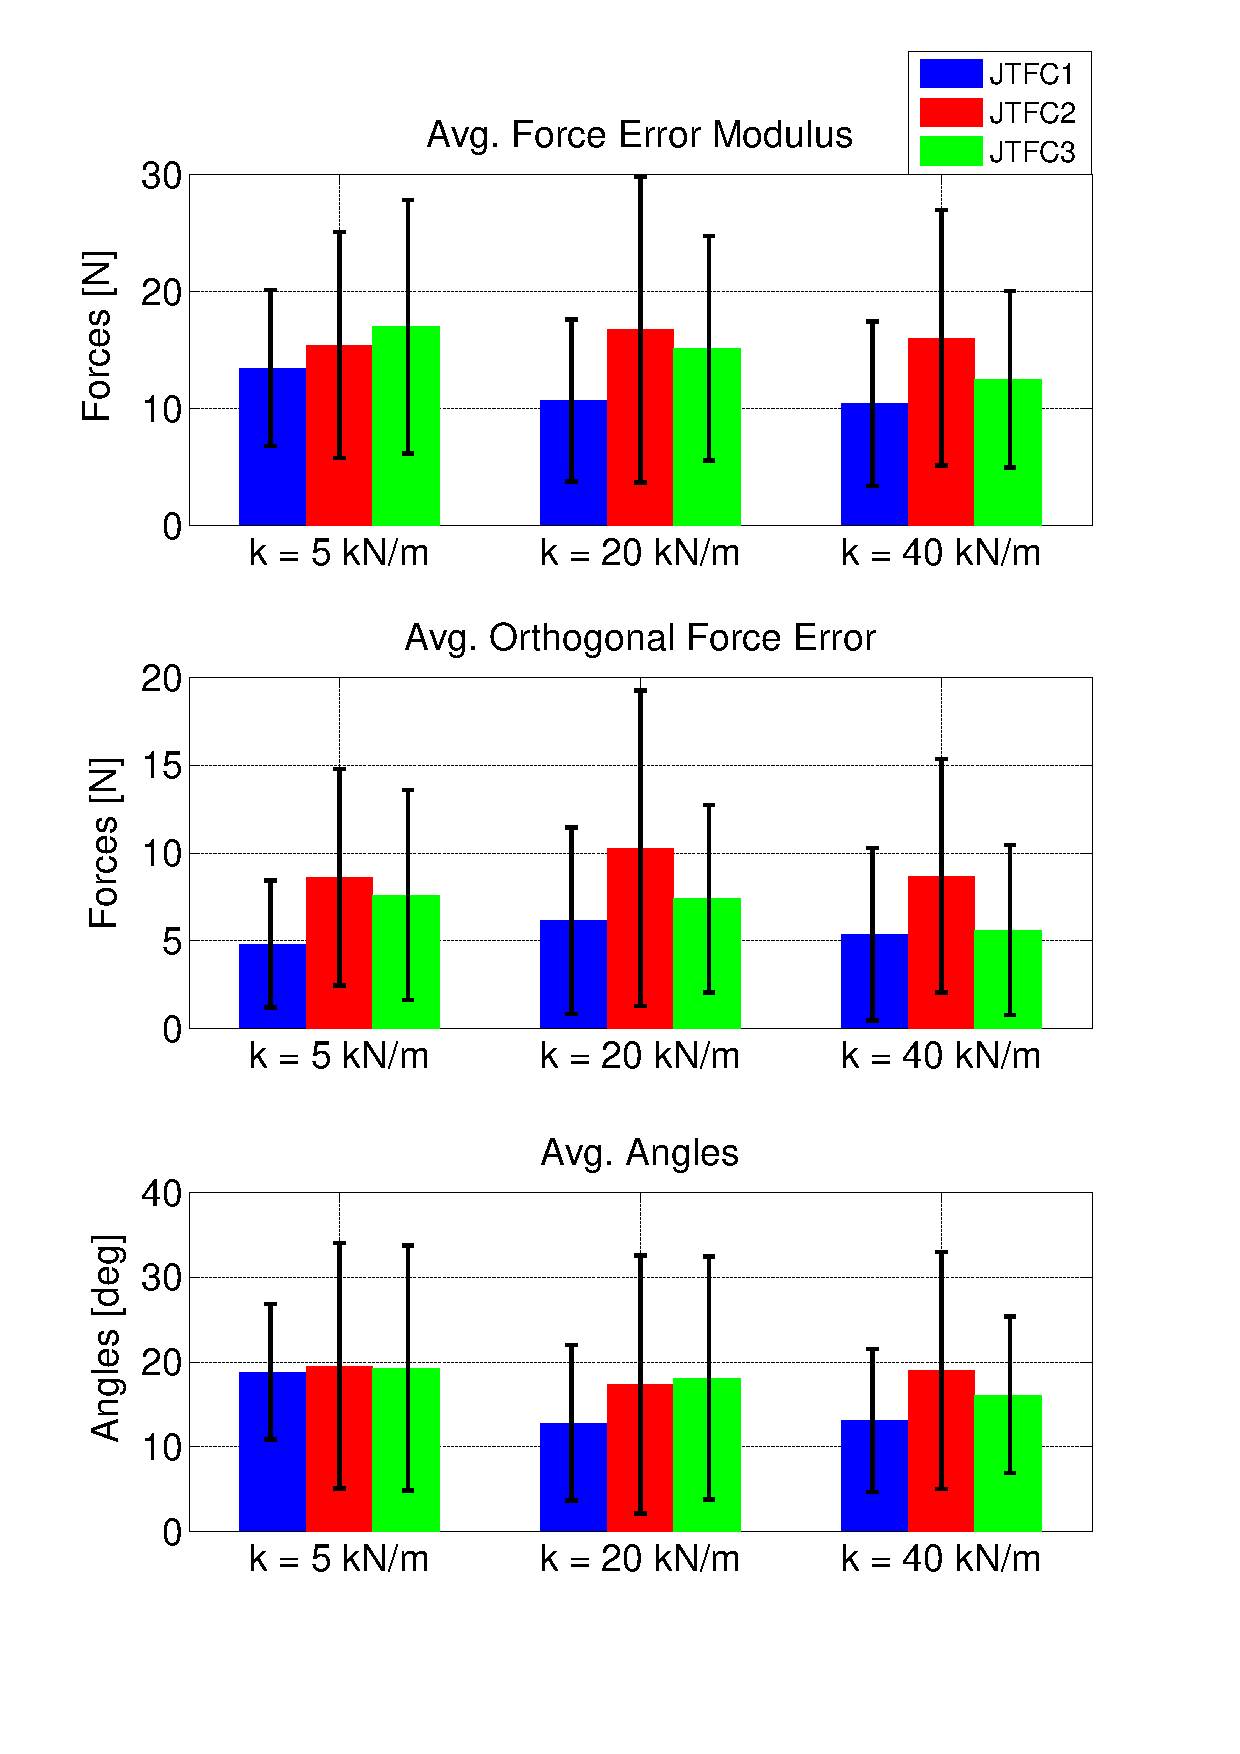
\includegraphics[width=1\columnwidth]{erroriForzeAngoliRendering}
	\caption{At the top, the average of the modulus of the error force vectors at the end effector of the 3 controllers in the rendering task. For this test, 3 stiffness has been evaluated: 5kN/m (small), 20 kN/m (medium) and 40 kN/m (high). In the middle, the average error forces of the orthogonal component. At the bottom, the average angle between the desired force vectors and the measured ones.}
	\label{fig:renderingErrors}
\end{figure}

\par The results can be shown in the \figurename \ \ref{fig:renderingErrors}. The first graph shows the average difference between the rendered forces by the controls and the desired forces with an aggregate index, i.e. the norm of the error vector. From this graph the reader can see that in all the condition the JTFC1 control performs better then the others, in fact the mean of the error is around 10 N in all the three cases.
\par To decompose the informations given in the first graph, other two indexes are considered, that are the average error of the orthogonal component of the force and the angle between the desired and the rendered forces. Unlike the norm of the error vector, these two indexes give information on the amplitude and the direction of the undesired force components. The second graph highlights that the JTFC1 control leads to an average error of 5 N along the task direction independently from the environment parameters, that is a good result coupled with the exhibited stable contact with the surface in every condition.
The third graph is substantially in agreement with the previous ones.

%%%%%%%%%%%%%%%%%%%%%%%%%%%%%%%%%%%%%%%%%%%%%%%%%%%%%%%%%%%%%%%%%%%%%%%%%%%%%%%%%%%%%%%%%%%%%%%%%%%%%%%%%%%%%%%%%%%%
%%%%%%%%%%%%%%%%%%%%%%%%%%%%%%%%%%%%%%%%%%%%%%%%%%%%%%%%%%%%%%%%%%%%%%%%%%%%%%%%%%%%%%%%%%%%%%%%%%%%%%%%%%%%%%%%%%%%
%%%%%%%%%%%%%%%%%%%%%%%%%%%%%%%%%%%%%%%%%%%%%%%%%%%%%%%%%%%%%%%%%%%%%%%%%%%%%%%%%%%%%%%%%%%%%%%%%%%%%%%%%%%%%%%%%%%%
%%%%%%%%%%%%%%%%%%%
%DIFDELCMD < %%%
\DIFdelend \DIFaddbegin \section{Introduction}

Exoskeletons are robotic interfaces for human-robot interaction where the highest physical symbiosis with the human operator is achieved 
\cite{Frisoli2019Encylopedia}.
%\hldoing{insert here wearable robots citation from encylopedia of robotics}
Unlike many industrial robots  designed to exhibit a stiff structure and behavior,  therefore to be used with a rigid position control, the exoskeletons are in direct contact with humans, so that  they have to satisfy  safety and compliance requirements common to physical Human-Robot Interaction (pHRI) devices \cite{bajcsy2017learning}.
\par In physical Human-Robot Interaction applications, moreover  there are other performance measures inherently depending on the actuation and control that need to be considered, among which the two most relevant ones are {\em transparency} and  {\em haptic rendering}: 

%
%\begin{description}[\setlabelwidth{$\alpha\omega\pi\theta\mu$}\usemathlabelsep]
%	\item[$\gamma\delta\beta$] Is the index of..
%	\item[$\alpha\omega\pi\theta\mu$] Gives the....
%\end{description}
	
%	[\setlabelwidth{Haptic rendering}]
\noindent
%\setlength{\IEEEdlabelindent}{-0.5 \parindent}
\setlength{\IEEEiednormlabelsep}{-2 \parindent}
\begin{IEEEdescription}
	%[\IEEEsetlabelwidth{Very long label} \IEEEusemathlabelsep]
	\item[{\bf Transparency }] \hspace{2 cm}
	%Transparency
	 relates to the ability of the
	robotic system interacting with a human who is moving
	voluntarily
	not to apply any assistance/
	resistance to free motion
	\cite{jarrasse2010methodology},
	or equivalently means that the robot’s
	reaction forces perceived by the user are minimal \cite{just2018exoskeleton}.
	No standard procedures exist for the measurement of transparency in pHRI, but for exoskeletons there is a general consensus  to refer not only to end-effector resistance forces, but also to single joints resistance torques or measurements at contact points \cite{just2018exoskeleton}.
	\item[{\bf Haptic rendering} ] %\hspace{2 cm}
	 %Haptic rendering 
	 \hspace{2.7 cm}
	  refers to the capability of the device to render a desired dynamic behavior, such as a virtual impedance  or a virtual wall, i.e. a
	task featuring both very high impedance (when in contact
	with the wall) and very low impedance (when out of
	contact) \cite{colgate1994factors}. Better mechanical structures,
	including appropriate dimensioning of the sensors and
	actuators, combined with more effective
	control strategies  should predict the maximum
	stiffness that can be displayed by existing devices   \cite{diolaiti2005criterion}.
\end{IEEEdescription}


In the last two decades, several exoskeleton solutions have been proposed using different implementation principles according to the field of application, such as  neurorehabilitation and assistance \cite{lo2012exoskeleton,pirondini2016evaluation,xiloyannis2019physiological}, human power augmentation \cite{kim2016powered}) and telepresence \cite{buongiorno2018wres, rebelo2014bilateral,buongiorno_chiaradia_marcheschi_solazzi_frisoli_2019}, where different actuation systems and technologies have been exploited, based on geared solutions \cite{mihelj2007armin,vertechy2009development,carignan2005design}, tendon drives \cite{frisoli2009force,perry2007upper}, hybrid solutions \cite{garrec2008able,onTheEdgeTiseni19}, pneumatic or hydraulic  actuation \cite{tsagarakis2003development,klein2010optimization}.

% can be found in literature.

% to enhance the master immersivity and dexterity.
%
%Intro sulle architetture di giunto dove si illustrano le diverse tipologie, dove si contestualizza la nostra scelta e si motiva la nostra scelta.
%\par In physical Human-Robot Interaction (pHRI) devices, 


%%%compliance of actuator temporary removed
As shown in  \figref{fig:exosActuators}, the actuators found in recent exoskeletons and humanoids for pHRI  can be mainly classified in two main categories, the {\em active impedance by control} and {\em inherent impedance }  (compliance, damping) according to how they adjust the impedance displayed to the user, obtained  either by control in the first case or as a mechanical property in the second case 
\cite{vanderborght2013variable}. %% shows a scheme of the two variable impedance typologies.


% in two main categories, variable impedance actuators (VIA) and stiff actuators suitable for position control strategies. For pHRI the use of purely position controlled solutions is of limited interest. On the other hand,
\begin{figure}[]
	\centering
	%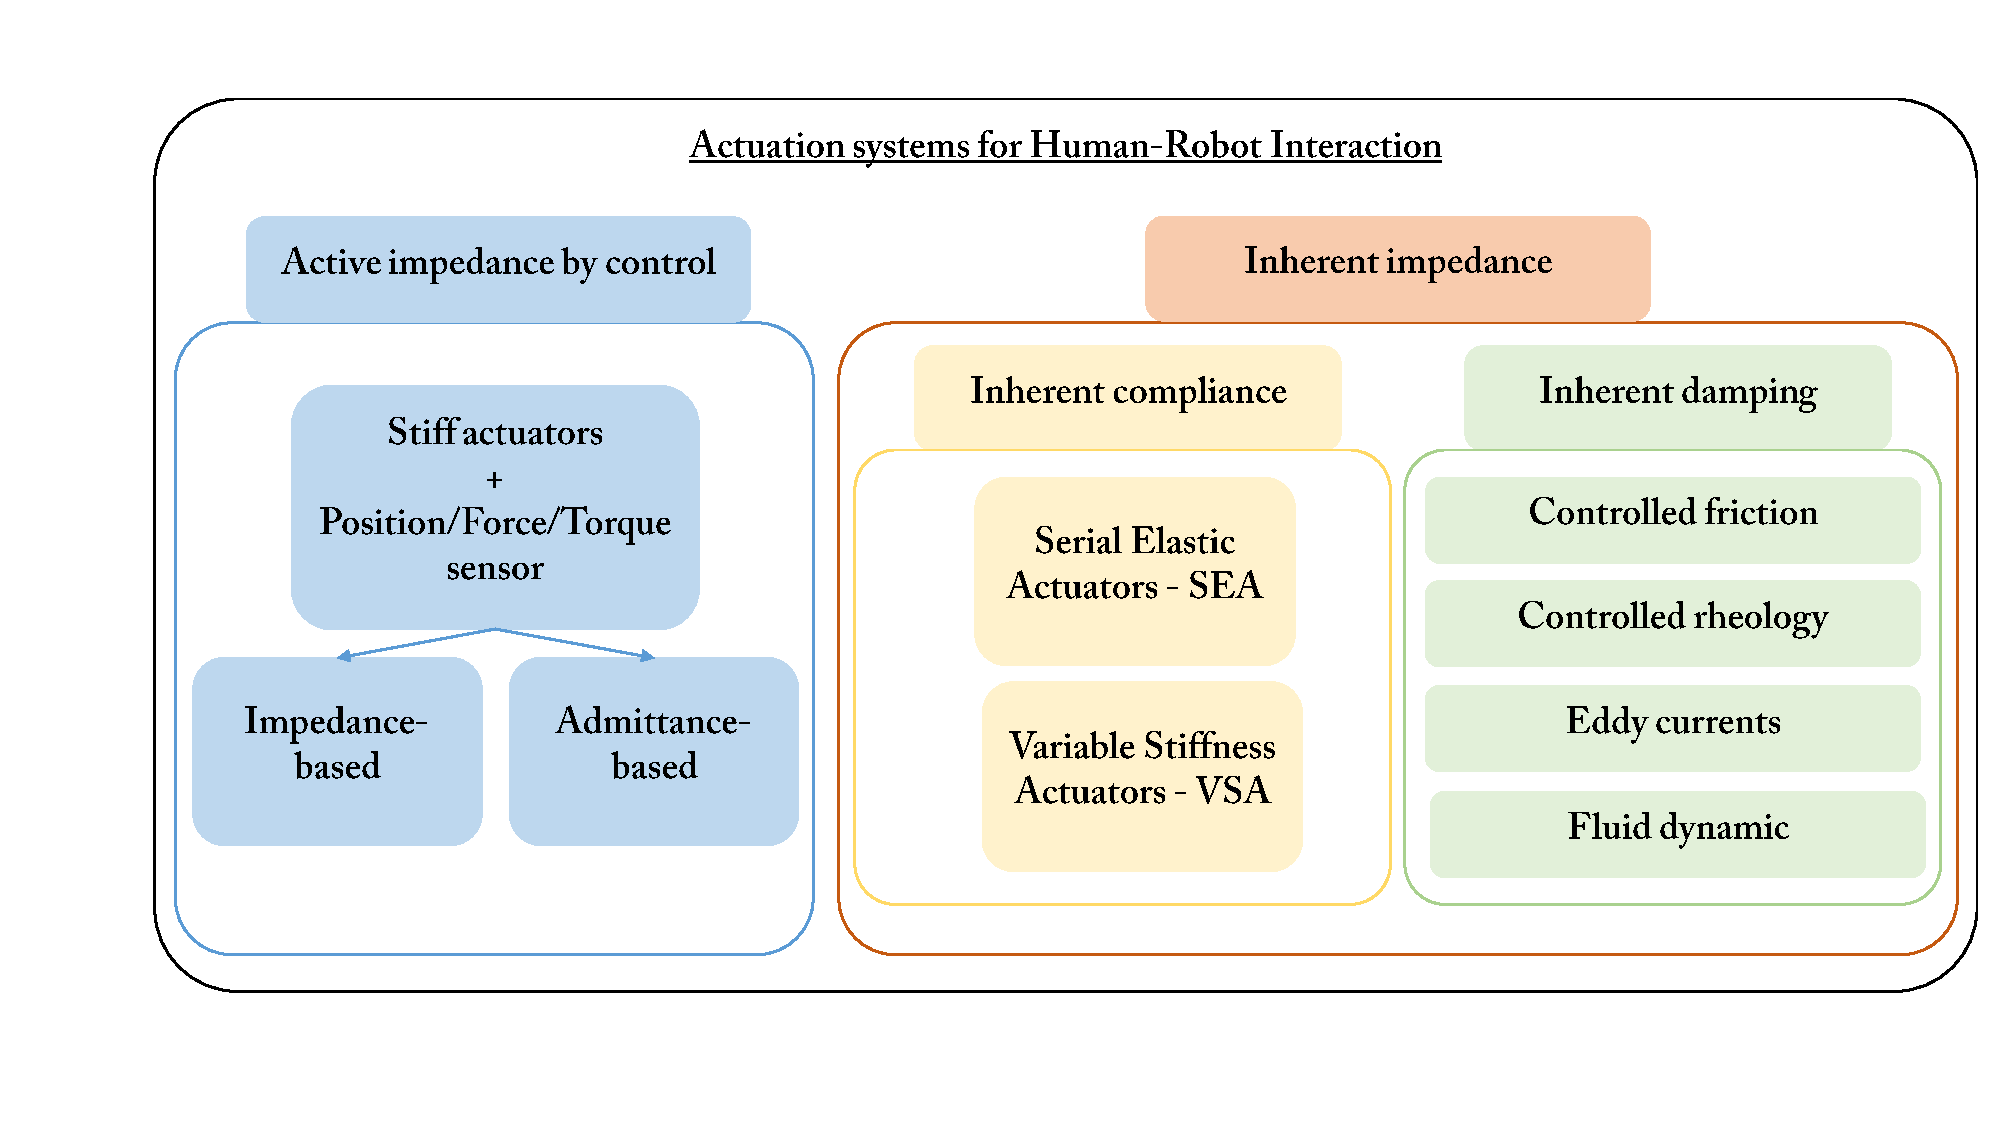
\includegraphics[width=1 \columnwidth]{actuators}
	\def\svgwidth{1\columnwidth}
	\begin{footnotesize}
		\input{imgRevised/SoA.pdf_tex}
	\end{footnotesize}
	\caption{Schema of variable impedance actuation systems for human-robot interaction. The impedance can be simulated and  actively changed by control (this relies on position and torque sensors) or can be an inherent mechanical property of the actuator. In the latter case the mechanical stiffness can be a fixed value (SEA) or can be adjusted (VSA), and the damping can be controlled.}
	\label{fig:exosActuators}
\end{figure}
%
\par In {\em  inherent compliance } actuators an electric motor is coupled with a spring with fixed (Series Elastic Actuator - SEA) or variable stiffness (Variable Stiffness Actuators - VSA), based on the principle that  adding a series elastic element reduces the peak power demand to the motor. {\em Inherent damping } actuators are based on the control of the friction by means of eddy currents, controlled rheology or fluid dynamics. 
%Recently double actuation architectures have been developed for variable impedance actuators	\cite{tagliamonte2012double}, coupling a stiff motor in parallel with an elastic element (Parallel Elastic Actuators - PEA).  Both SEA and VSA have been implemented in exoskeleton as for example in Lopes \cite{veneman2007design}, an exoskeleton for the gait assistance that is based on SEA actuation, or in NEUROexos elbow exoskeleton \cite{vitiello2013neuroexos} that is based on VSA and in ALTACRO locomotion exoskeleton \cite{cherelle2010maccepa} that introduces a Mechanically Adjustable Compliance and Controllable Equilibrium Position Actuator (MACCEPA).
%. 
% 

%Recently double actuation architectures have been developed for variable impedance actuators	\cite{tagliamonte2012double}, coupling a stiff motor in parallel with an elastic element (Parallel Elastic Actuators - PEA).  
Both SEA and VSA have been implemented in exoskeleton as for example in Lopes \cite{veneman2007design},  in NEUROexos elbow exoskeleton \cite{vitiello2013neuroexos}and  ALTACRO locomotion exoskeleton \cite{cherelle2010maccepa}.

All the variable impedance actuators have the advantage of absorbing impacts and SEA and VSA % (inherent compliance) 
can eventually mechanically store energy during passive phases and release it in active phases of the movement cycle.  VSAs generally use two motors which increases the size, weight and complexity of the actuator in comparison with an SEA \cite{wolf2011dlr}.

\par On the other side, {\em active impedance by control}  actuators are composed of electric motors coupled with a transmission/reduction system; they can be classified
according to the backdrivability and sensing system. Force controlled actuators implement a force/torque sensor
at the joint level and can achieve impedance behavior by closed-loop control.
In general traditional actuators with no elastic or damping elements can be lighter and more compact
than passive variable impedance actuators, but their time response and dynamic bandwidth is limited by control and electrical properties of actuators, such as maximum velocity of electrical motor.
%
%The actuation system influences the control design: active exoskeletons can be classified as impedance based design (open-loop impedance control \cite{frisoli2009force} and impedance control with force feedback) or admittance-based design (admittance control with position feedback) \cite{carignan2000closed}.
%
%Open-loop impedance control exoskeletons rely on lightweight designs with joint-delocated motors and backdrivable mechanical solutions, typically implemented making use of tendon transmissions \cite{frisoli2009force}, \cite{perry2007upper}; the most challenging limitations are the friction effects due to the transmission system, that can be compensated only by means of feed-forward compensation based on approximate models, the complexity of the transmission and the difficulty to be mechanically configured in a bilateral configuration, working both for left and right arm. 
%On the other side admittance-based design requires force sensing and can achieve higher stiffness values, but relies on the adopted control for canceling system dynamics and inertia.
%Exoskeleton with a single force/torque sensor localization, such as one torque sensor at the exoskeleton elbow joint and a six-axis force/torque sensor at the exoskeleton handle \cite{carignan2008controlling} or shoulder \cite{nef2007armin}, can accurately regulate interaction forces at the exoskeleton terminal link (i.e. the handle) only.
%Lightweight robots with joint torque sensors \cite{albu2007dlr} allow for multi-contact force/torque control (i.e. the regulation of interaction force/torques at multiple points distributed over multiple links).
%
%
%The correct estimation of interaction force between human and exoskeleton in admittance designs requires control approaches that compensate for friction, inertial and gravity properties of the exoskeleton mechanical structure, but  a complete cancellation of these effects is  difficult to achieve.
%

%
%\begin{figure}[htb]
%	\centering
%	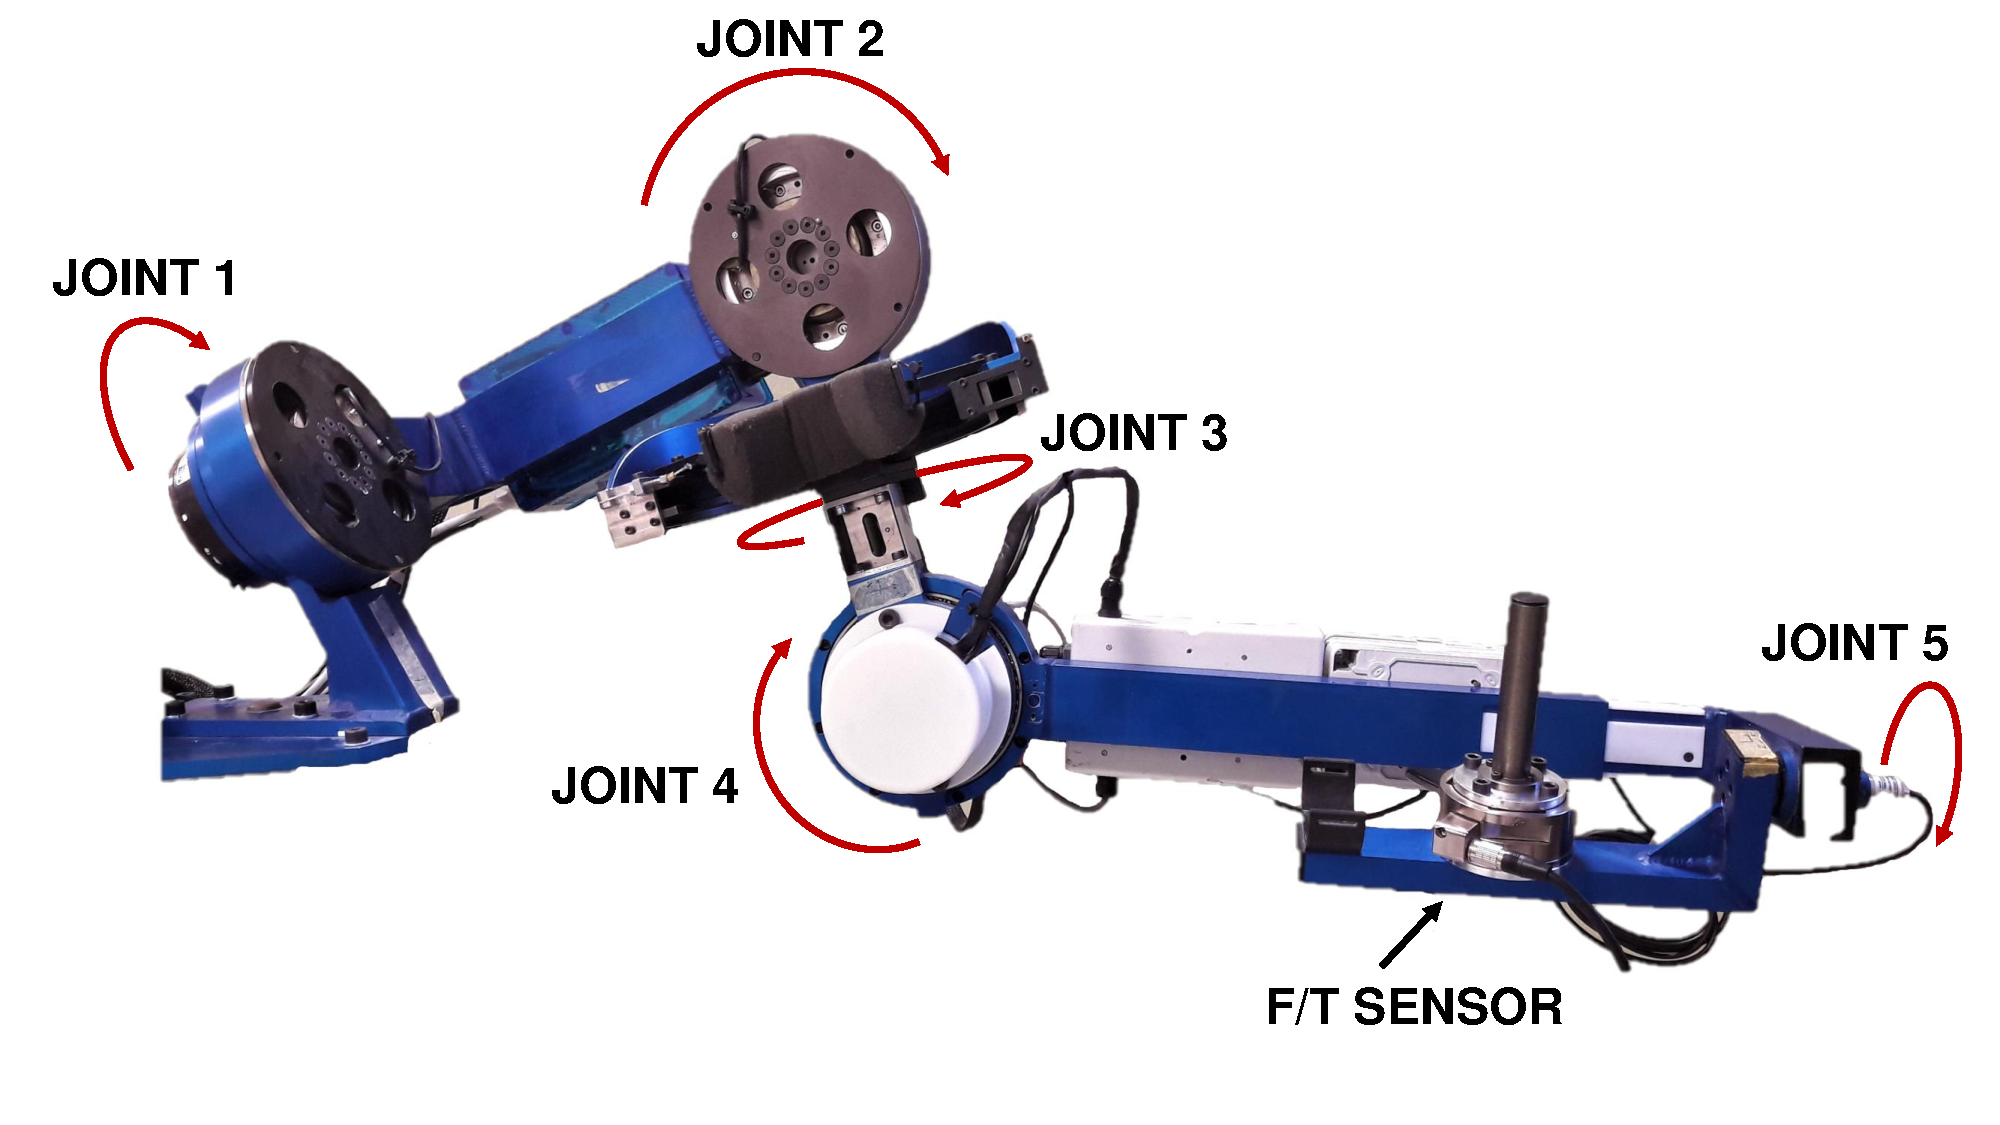
\includegraphics[width=0.95\columnwidth]{RehabDescription} 
%	\hldoing{insert here SoA transparency and issues}
%	\caption{The Rehab-Exos. It is a 5 DOF upper-limb exoskeleton  with 4 actuated joints. The joints $J_1$, $J_2$ and $J_4$ share the same characteristics: high reduction ratio (100:1) by means of harmonic drive, embedded torque sensor and maximum actuation torque of 150 \ Nm. The joint $J_3$ is composed by a semi-circular guide actuated by a DC motor through tendon transmission. Joint $J_5$ is passive and the exoskeleton is equipped of a force/torque sensor at the end-effector that is used for evaluation purposes.}
%	\label{fig:rehabexos1} 
%\end{figure}
%
\par Solutions based on joint torque sensor have been proposed in the last years mostly for example in  lower limb exoskeletons  \cite{kim2015design,aguirre2011design,hwang2015method}. 
%In  \cite{kim2015design} \cite{kim2015design,aguirre2011design,hwang2015method} and in \cite{aguirre2011design} two knee exoskeletons based on joint torque sensor were presented; the latter exoskeleton implements an admittance control based on the torque sensor readings. In \cite{hwang2015method} the torque sensor for a lower limb exoskeleton allows it to accurately estimate the human muscular torque that were exerted during the human-robot interaction. 
The advantage of joint torque sensor based solutions is their compactness and robustness, but when the torque sensor is embedded in the joint it is sensitive to the link inertia in addition to the human interaction torques, thus affecting the system {\em transparency}. A mechanical solution is presented in \cite{zanotto2013improving} where the transparency of a lower-limb exoskeleton has been improved by positioning the force/torque sensor on the supporting cuffs, that is at the interaction point between the human leg and the exoskeleton.
%%%%%%%%%COMMENTED BY ANTONIO IN SECOND REVISION
%%\par Even if SEA and VSA are less compact then traditional actuators, for example \cite{cestari2014ares} \hldoing{not clear here} proposed a solution based on a VSA for an exoskeleton of the leg that reduced the lateral size and integrates a torque sensor based on spring's deflection reads.
 Sensors used to measure these deflections are generally encoders \cite{dos2017design} and potentiometers \cite{junior2016series}; the latter usually require custom mechanical supports to avoid errors related with its sensitivity to misalignments.
While the deflection based force estimation becomes a most widely utilized method for the SEAs and VSAs and performs fidelity force control performance in various robotic applications, there are still difficulties because of the practical issues such as spring deflection measurement error or noise of the encoder signal \cite{lee2018integrated}. These factors have much negative impact on SEA with high stiffness. In \cite{leal2018polymer}, for example, a polymer optical fiber has been mounted on the torsional spring of a SEA to read angles and torques in a more accurate way without considerably enlarging the size of the actuator at the cost of a more specific system electronics.
\par Thus, the adoption of inherent compliant actuation systems rather than achieving compliance by control  is not a trivial choice and it depends on the desired mechanical features and is the result of a trade-off among compactness, weight, simplicity, costs, safety, efficiency.
A good trade-off that prefer compactness, simplicity and uses just one motor is an active impedance by closed-loop control  system that  an elastic component to transmit and to measure axial torques at the same time.


%, extending our previously work presented in \cite{solazzi2014interaction}
\par 
Based on the above, in this paper 
%we address the issue of  collaborative robot behavior,
we introduce the design and the experimental characterization of the Rehab-Exos, an upper limb exoskeleton endowed with  joint torque actuators, based on  joint torque sensors and high reduction ratio, and the design of an  interaction joint torque controller that maximizes both  {\em transparency } and  quality of {\em haptic rendering}.

%The overall control design was optimized and experimentally verified to compare the obseved performance  with two other interaction joint torque architecture used as benchmarking.

%The Rehab-Exos allows to obtain a physical interaction characterized by good {\em transparency } and  quality of {\em haptic rendering}, it is capable to exert a wide range of forces and at the same time it exhibits high position accuracy due to high gear reduction ratio.

\par In particular, to improve transparency we propose a new interaction state-feedback torque controller (JTFC1) that takes into account the multi-dof non linear system dynamics and provides a compensation of other non-linear effects, such as friction and gravity components, to achieve an accurate estimation of human interaction force.
This is accomplished by a single joint optimum observer that ensures joint torque tracking, while a centralized controller estimates and compensates for the dynamics of the whole system. 
%Moreover, we have evaluated the effect of dynamic compensation on system transparency highlighting good results.
\par To validate the proposed controller as well as the chosen mechanical architecture, the full-state feedback controller was  compared with two alternative controllers,  a  feedback controller (JTFC2) and a passivity-based feedback controller (JTFC3), in two tasks: the zero desired force tracking ({\em transparency}) and the contact with a virtual stiff wall ({\em haptic rendering}). 
The {\em transparency} benchmarking test among the 3 controllers was performed experimentally with 10 subjects and two different reference velocities, according to the evaluation procedure already tested in \cite{just2018exoskeleton}, in order to achieve comparable benchmark results.

As far as haptic rendering, the stability behavior and quality of force rendering of the proposed controller was assessed through a virtual wall simulation implemented with increasing  stiffness values and  compared it with the other two  benchmark controllers.
In  both experimental conditions,  the proposed joint torque controller allows it to achieve higher performance both in term of transparency and haptic rendering, demonstrating how an active impedance by control  can reach optimal performance if suitable state feedback is employed.
%Results reward the chosen mechanical and control strategy as presented in the last part of this paper.


%\par The first part of the paper widely treats the critical issue due to the use of a torque sensor embedded in the joint and in particular the sensitivity to non-axial load has been studied. Then, in the second part the joint model and the control technique are presented.

\par This paper is structured as follows: Section \ref{sec:systemDesign} presents the design of the Rehab-Exos with a particular focus on the strain gauge-based torque sensor design and issues. Section \ref{Single joint model} provides a mathematical model of the single joint whereas in the Section \ref{Full dynamics model} the full dynamics model of the Rehab-Exos is described. Section \ref{sec:Full_state_feedback_controllers} explains the proposed full state feedback controller and recalls two benchmark torque controllers already known in literature. Section \ref{sec:experimentsResults} presents the experiments and the obtained results.
Finally, discussions and conclusions are addressed in Sections \ref{sec:discussion} and \ref{sec:conclusion} respectively.  

%
%Active exoskeleton systems are robotic devices that can be worn on the user's body, implying that they should satisfy requirements of safety and better compliance.
%After the Fukushima event in Japan, the application of these human-robot interfaces in the area of rescue robotics and teleoperation has became an emerging field of research,
%for which the development of upper limb active exoskeletons with dexterous manipulation abilities has become a hot topic of research.
%Another relevant sector of application of active exoskeletons is represented by neuro-motor rehabilitation post-stroke \cite{lo2012exoskeleton}, where different prototypes and commercial solutions have been recently proposed.
%
%
%While the general rationale for the design of high performance haptic interfaces are the satisfaction of the requirements of high force fidelity, transparency
%and backdrivability, specific issues need to be addressed in exoskeleton design in terms of safety, kinematics and ....
%
%For what concerns, upper limb exoskeletons, we should consider:
%\begin{description}
%\item[User requirements] Safety: the structure is always in close contact with the user
%\item[Design issues, kinematics, mechanical design]
%The kinematics should be adjusted to user arm, Possibility of adjusting the size of the system to avoid internal forces
%Complexity of shoulder motion, Non periodicity of upper limb movement compared to lower limb, Intrinsic 3D spatial motion Both left and right arm schemes should be implementable
%\item[Design issues, control] Low inertia should be achieved, possibility of employing force sensors, Remote vs. local actuation, High forces required (no gravity cancellation provided by support elements e.g., support plans)
%\end{description}
%
%%In SSSA there is a consolidated experience in the design and development of new exoskeleton systems \cite{frisoli2005new}, as shown in figure~\ref{fig:exos@SSSA}.
%
%%%%%%%%%%%%%%%%%%%%%%%%%%%%%%%%%%%%%%%%%%%%%%%%%%%%%%%%%%%%%%%%%%%%%%%%%%%%%%%%%%%%%%%%%%%%%%%%%%%%%%%%%%%%%%%%%%%%
%%%%%%%%%%%%%%%%%%%%%%%%%%%%%%%%%%%%%%%%%%%%%%%%%%%%%%%%%%%%%%%%%%%%%%%%%%%%%%%%%%%%%%%%%%%%%%%%%%%%%%%%%%%%%%%%%%%%
%%%%%%%%%%%%%%%%%%%%%%%%%%%%%%%%%%%%%%%%%%%%%%%%%%%%%%%%%%%%%%%%%%%%%%%%%%%%%%%%%%%%%%%%%%%%%%%%%%%%%%%%%%%%%%%%%%%%
%%%%%%%%%%%%%%%%%%%%%%%%%%%%%%%%%%%%%%%%%%%%%%%%%%%%%%%%%%%%%%%%%%%%%%%%%%%%%%%%%%%%%%%%%%%%%%%%%%%%%%%%%%%%%%%%%%%%


\section{System design} \label{sec:systemDesign}
%\hldone{Done}
\begin{figure*}[htb]
	\centering
	%	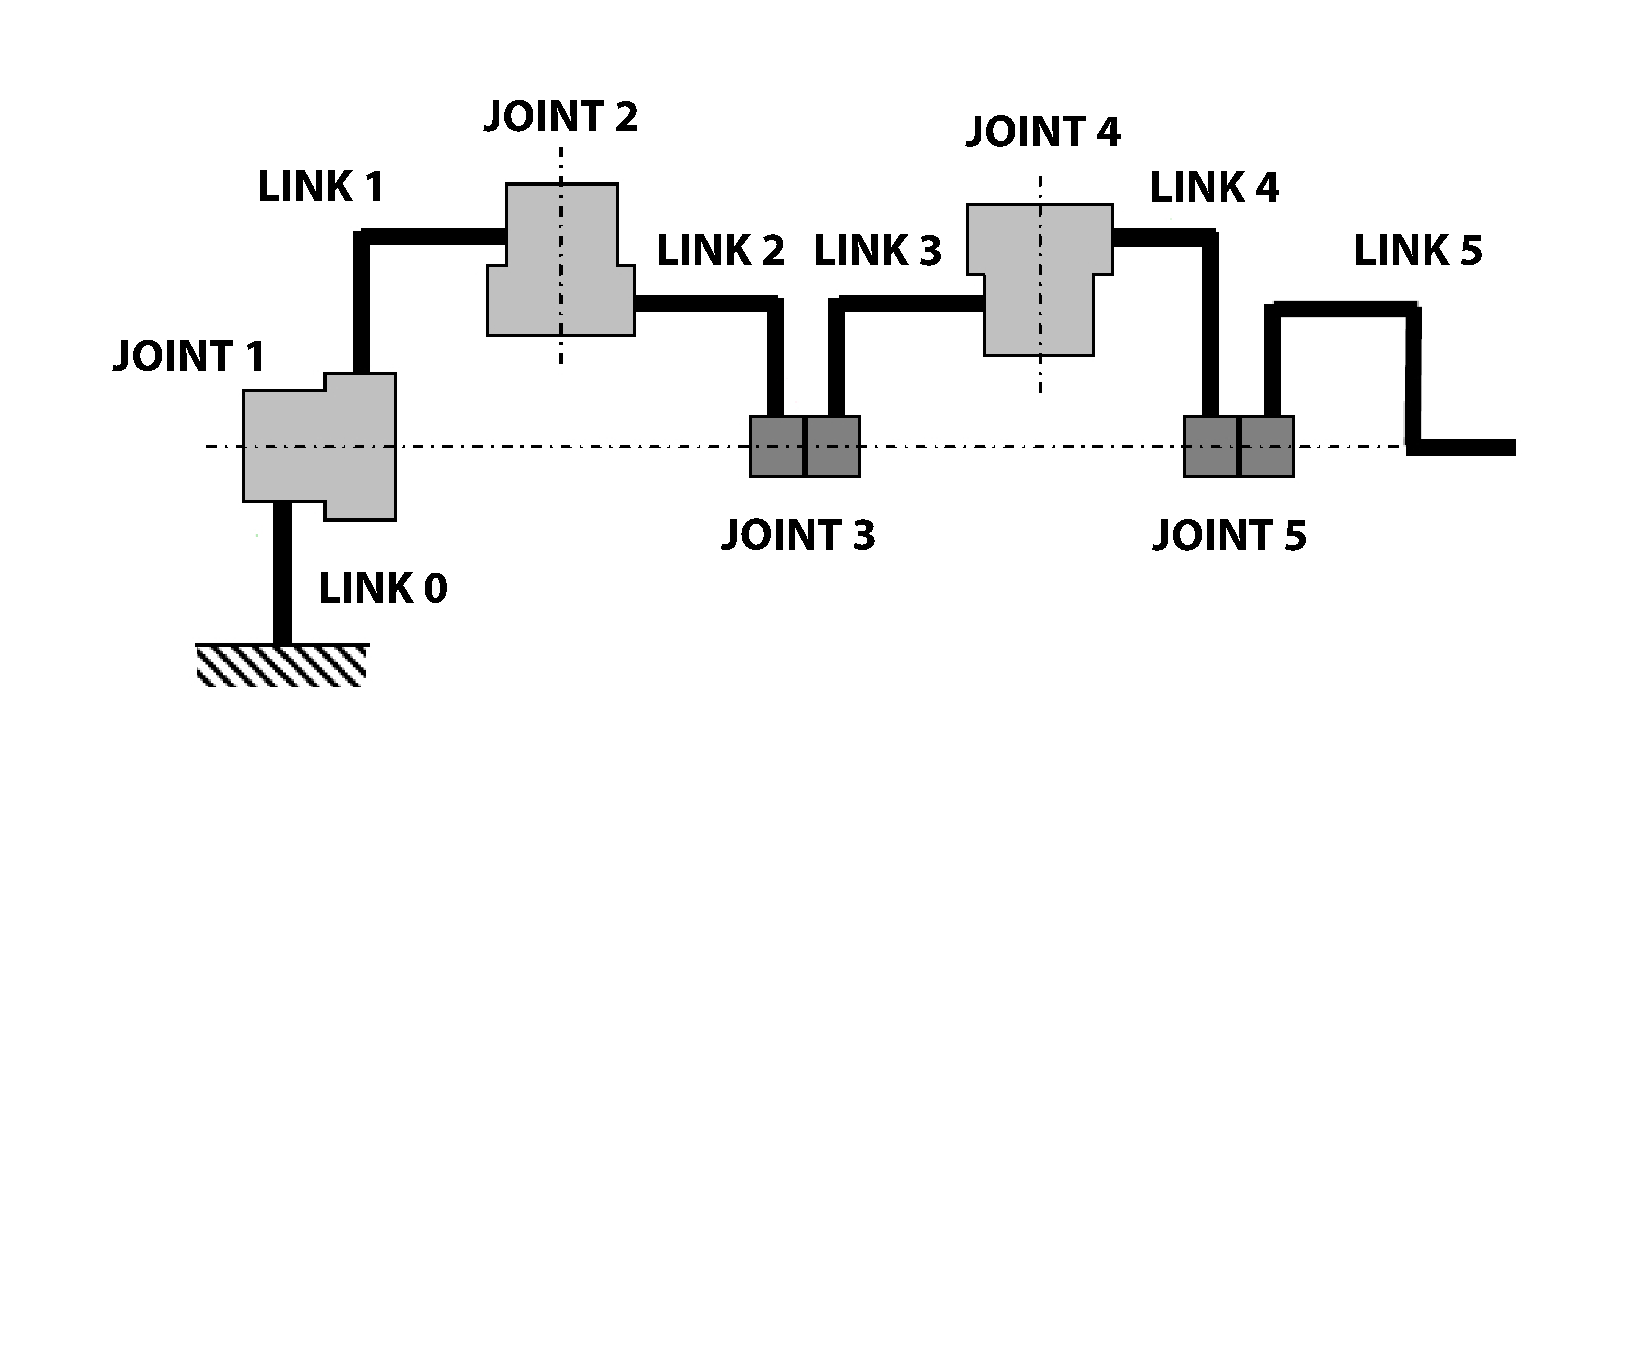
\includegraphics[width=0.9\columnwidth]{SchemaExos}
	\def\svgwidth{2\columnwidth}
	\begin{footnotesize}
		\input{imgRevised/rehab_description.pdf_tex}
	\end{footnotesize}
	\caption{(a) The Rehab-Exos. It is a 5 DOF upper-limb exoskeleton  with 4 actuated joints. The joints $J_1$, $J_2$ and $J_4$ share the same characteristics: high reduction ratio (100:1) by means of harmonic drive, embedded torque sensor and maximum actuation torque of 150 \ Nm. The joint $J_3$ is composed by a semi-circular guide actuated by a DC motor through tendon transmission. Joint $J_5$ is passive and the exoskeleton is equipped of a force/torque sensor at the end-effector that is used for evaluation purposes. (b) A schematic representation of the Rehab-Exos exoskeleton. (c) CAD section of the $J_1$, $J_2$ and $J_4$ joint actuator of the Rehab-Exos. (d) Characteristic dimensions of the torque sensor.}
	\label{fig:rehabexosSchema}
\end{figure*}

The Rehab-Exos is an active robotic exoskeleton (\figurename \ \ref{fig:rehabexosSchema})  designed with the idea to be modular, easily reconfigurable and with a good trade-off between transparency and force payload.
It was conceived for rehabilitation applications and it is designed in such a way to generate controlled contact forces/torques not only at its end-effector handle, but also at  intermediate contact points with the user arm. When the user is wearing the device he can control the full force interaction with the exoskeleton and guide/be guided by shoulder and elbow) articulations of the arm. 
The physical interaction between user and exoskeleton is monitored by the joint torque sensors, and their performance depends on several design and implementation aspects that are addressed in subsection \ref{subsec:DesignTorqueSensor}.
%%%%%%%%%%%%%%%%%%%%%%%%%%%%%%%%%%%%%%%%%%%%%%%%%%%%%%%%%%%%%%%%%%%%%%%%%%%%%%%%%%%%%%%%%%%%%%%%%%%%%%%%%%%%%%%%%%%%
%%%%%%%%%%%%%%%%%%%%%%%%%%%%%%%%%%%%%%%%%%%%%%%%%%%%%%%%%%%%%%%%%%%%%%%%%%%%%%%%%%%%%%%%%%%%%%%%%%%%%%%%%%%%%%%%%%%%
\subsection{Mechanical design of the Rehab-Exos} 
%\hldone{Done}
\label{subsec:mechanicalDesign}
As depicted  in \figurename \ \ref{fig:rehabexosSchema}, the exoskeleton has a serial architecture isomorphic with the human kinematics that comprises: a shoulder joint  fixed in space and composed by three active joints $J_1$, $J_2$ and $J_3$; an active elbow joint $J_4$; and a passive revolute joint $J_5$ allowing  wrist prono/supination.  For a more detailed description of both Rehab-Exos and actuation groups, the reader can refer to \cite{vertechy2009development}.
%\begin{figure}[htb]
%	\centering
%	\subfigure[Exoskeleton kinematics]{\includegraphics[width=0.49\columnwidth]{\figpath{exos1}}\label{fig:exos_kinematics}}
%	\subfigure[CAD section of the joint actuator ]{\includegraphics[width=0.49\columnwidth]{\figpath{JointActuator}}\label{fig:exos_actuator}}
%	\caption{The Rehab-Exos CAD model showing overall kinematics and actuator structure}
%\end{figure}

%
%
%\begin{figure}[]
%	\centering
%	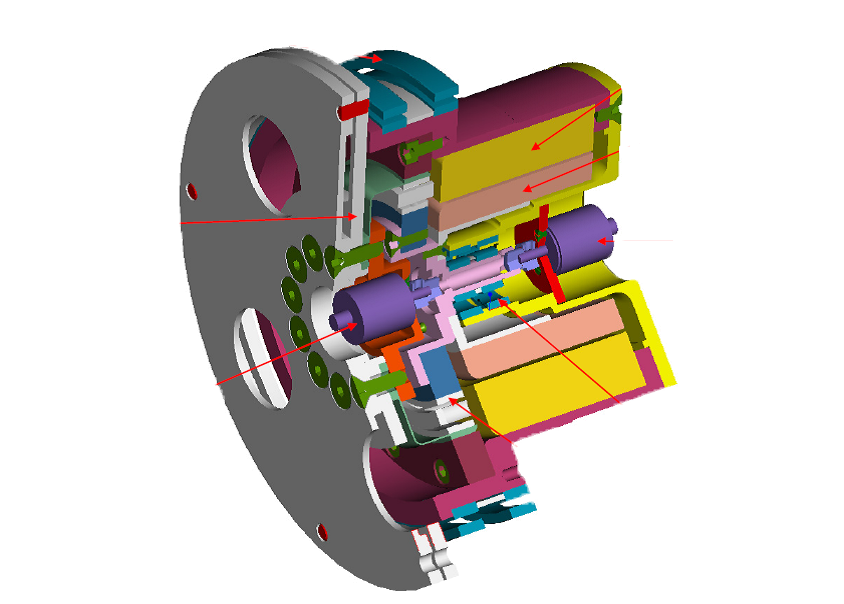
\includegraphics[width=0.7\columnwidth]{JointActuator}
%	\caption{CAD section of the $J_1$, $J_2$ and $J_4$ joint actuator of the Rehab-Exos.}
%	\label{fig:exosActuatorCAD}
%\end{figure}
%
\par The three joints $J_1$, $J_2$ and $J_4$ of the exoskeleton are motorized through identical actuation groups. Each joint features a custom-made frameless brushless torque motor integrating a compact Harmonic Drive (HD) component set. The actuator provides a joint output torque equal to $150\ Nm$ with an overall weight equal to $3.7\ Kg$ and a motor shaft inertia reduced to the joint output shaft $Jm = 2.5 \ Kgm^2$. The Harmonic Drive performs a reduction equal to 100:1. Due to the adopted mechanical components, the joints feature limited back-drivability at motor power-off and limited mechanical complexity to ease maintenance as well as reduce costs. A CAD section of the $J_1$, $J_2$ and $J_4$ joints is depicted in \figurename \ \ref{fig:rehabexosSchema} c).
Joint $J_3$ is characterized by a tendon transmission that is used to transmit the actuation torque through an open semi-circular guide. More detail on the joint $J_3$ can be found in \cite{vertechy2009development}.

\subsection{Design aspects of the strain gauge based torque sensor}
%\hldone{Done}
\label{subsec:DesignTorqueSensor}
The three joints $J_1$, $J_2$ and $J_4$ have a torque sensor featuring a four-spoke-shape geometry. 
Despite further augmenting the actuation group compliance, the availability of joint-torque sensors enables multi-contact force control at multiple points distributed over the links and, additionally, makes it possible: 1) to close a stable high-bandwidth torque inner loop around each joint which is weakly affected by robot link variable inertia; 2) to suppress robot vibrations produced by the inherent transmission compliance (Harmonic Drive); 3) to reduce internal disturbance torques caused by actuator and reducer (for instance friction losses, actuator's torque ripples and gear teeth wedging actions); to measure externally applied forces/moments and complex non-linear dynamic interactions between joints and links.
\par The sensor consists of two fully balanced strain gauge bridges placed on different beams of the spoke, which is located at the joint output shaft. 
%
%
\begin{table}[t]
	\renewcommand{\arraystretch}{1.3}
	\caption{Characteristic dimensions of the torque sensor}
	\label{tab:sensorDimension}
	\centering
	\begin{tabular}{c c}
		\hline \hline
		\bfseries Dimension & \bfseries Value [$mm$] \\
		\hline
		R & 78 \\
		r & 38 \\
		L & 24 \\
		a & 4 \\
		round radius & 2 \\
		\hline \hline
	\end{tabular}
\end{table} 
%
%\begin{figure}[]
%	\centering
%	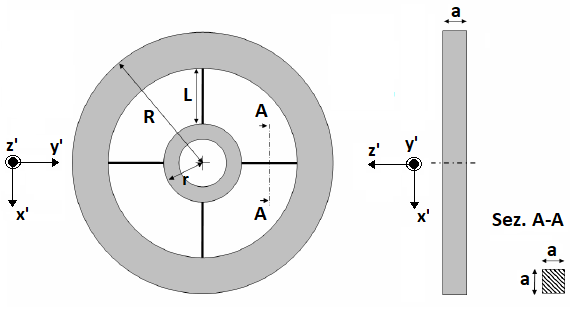
\includegraphics[width=0.7\columnwidth]{sensorDimensions}
%	\caption{Characteristic dimensions of the torque sensor.}
%	\label{fig:sensorDimensions}
%\end{figure}
%
The sensor is made by AISI 630 steel, harmonic steel exhibiting yield strength of 1950 MPa, Young's modulus of 196 GPa and has been dimensioned to exhibit low weight and high sensitivity to axial moments.
The axial torsional stiffness of the sensor is $k_s = 30$  kNm/rad and can be calculated as in \eqref{eqn:sensorStiffness}.
\begin{equation}
\label{eqn:sensorStiffness}
k_{s} = \frac{\tau}{\theta} = \frac{Ea^4(r+L(1-Q))}{3L^2(1/2-Q)}	
\end{equation}
where the adimensional parameter Q is given by
\begin{equation}
\label{eqn:adimensionalQ}
Q = \frac{3r+L}{6r+3L}	
\end{equation}
where, according to \figurename \ \ref{fig:rehabexosSchema} d), %$R$ is the radius of the external sensor ring, 
$r$ is the radius of the internal sensor ring, $L$ is length of the beams and $a$ is the side length of the beam section.
The characteristic dimensions of the sensor are reported in \tablename \ \ref{tab:sensorDimension}.
Moreover, the overall joint torsional stiffness reduced to the joint output shaft is $k = 11.38\ $kNm/rad.
\par The position of the strain gauges on the beam is a trade-off: if they were positioned in the middle of the beam the sensor sensitivity would be low, on the contrary, if they were positioned near the extremities the sensor reads would be affected by the non-linearities of the rounds of the beam. The selected distance from the extremities was $p = 1/8 \ L = 3$ mm.
To estimate the strain of the beam in a given point with distance $p$ from the inner ring under a certain axial torque $\tau$, the normal tension $\sigma_p$ that acts on that point $p$ needs to be computed as
\begin{equation}
\label{eqn:normalTensionOnBeam}
\sigma_p = \frac{3\tau((1-Q)L-p)}{2a^3((1-Q)L+r)}	
\end{equation}
and then the strain follow as 
\begin{equation}
\label{eq:strainEq}
\epsilon_A= \frac{\sigma}{E}
\end{equation} 
where $E$ is the Young's modulus.
\par Theoretically, i.e. using \eqref{eq:strainEq}, at $3 \ $mm  from the inner ring and under an axial torque of 120 Nm,  a maximum strain of $2.7\times 10^-3 $ m is obtained.
The same test has been conducted using a FEM software tool (Ansys\textregistered) because the surface of the strain gauge is not negligible compared to the beam one (see \figurename \ \ref{fig:strainGaugeDeformation}) obtaining a maximum strain of $1.98 \times 10^-3 $m.
The strain of each strain gauge when a $1 $Nm load is applied can be shown in \tablename \ \ref{tab:sensorStrain}.
\begin{table}[]
	\renewcommand{\arraystretch}{1.3}
	\caption{Strain of the 4 strain gauges}
	\label{tab:sensorStrain}
	\centering
	\begin{tabular}{c c c c}
		\hline \hline
		\bfseries Probe 1 [m] & \bfseries Probe 2 [m] & \bfseries Probe 3 [m] & \bfseries Probe 4 [m]\\
		\hline
		1.65e-5  & -1.33e-5 & -1.91e-5 & 2.2546e-5\\
		\hline \hline
	\end{tabular}
\end{table} 
%
\par An important characteristic of the torque sensor is the sensitivity to non-axial moments, thus an experimental test has been conducted to compute the sensitivity, i.e. a predetermined non-axial torque has been exerted on the sensor in 4 configurations (angle) of the sensor.
Experimental results are reported in \tablename \ \ref{tab:sensorNonAxialResults} and the sensitivity is equal to
\begin{equation}
S_S=\frac{C_{mis}}{C_S}=0.067
\label{eq:sensitivityToNonAxLoad}
\end{equation} 
%
\begin{table}[]
	\renewcommand{\arraystretch}{1.3}
	\caption{Sensor reads to non-axial moments}
	\label{tab:sensorNonAxialResults}
	\centering
	\begin{tabular}{cc}
		\hline \hline
		\bfseries Applied Torque [Nm] & \bfseries Sensor reads per angle [Nm]\\
		$\;$ &	\begin{tabular}{cccc} $0^\circ$   & $45^\circ$ & $90^\circ$ & $180^\circ$ \end{tabular} \\
		\hline
		32 & \begin{tabular}{cccc} 1.6 & 2.4 & 2.2 & 2.3 \end{tabular} \\
		64 & \begin{tabular}{cccc} 2.9 & 4.8 & 4.4 & 4.4 \end{tabular} \\
		96 & \begin{tabular}{cccc} 4.5 & 7.5 & 6.9 & 6.9 \end{tabular} \\
		\hline \hline
	\end{tabular}
\end{table} 
The sensitivity to non-axial moments is relatively high compared to one mentioned in \cite{kashiri2017sensor}. %This non-ideal and non-linear characteristic were not found in the initial test-rig, instead non-axial loads are there in the multi-link mounted exoskeleton. 
%Despite the presence of the ball bearings, two factors influence the sensor readings. The first factor is the way the mechanical parts are assembled (assembly errors), the second is the non-axial loads influence on the sensor readings. 
\par The reason of these results has been investigated and two causes (or a combination of them) have been proposed. The first cause of error could be a strain gauge mounting misalignment. The second cause could be an excessive deformation of the sensor due to the non-axial moments. 
About the first hypothesis, the sensitivity of the strain gauges to non-axial load $C_S$ (when a flexible model of the HD is considered) due to strain gauge misalignment can be modeled as
\begin{equation}
S_{misal}= k_s \cdot (k_{ex} \cdot e_x + k_{e\theta} \cdot e_{\theta})
\label{eq:sensitivityMisalignment}
\end{equation}
where $k_s$ is a scaling factor equal to $7.87e^{-3}$, $k_{ex}$ is the sensitivity to linear mounting misalignment  equal to $3$, $k_{e\theta}$ is the sensitivity to angular mounting misalignment equal to $2.3$, whereas $e_x$ and $e_{\theta}$ are the positional and angular misalignment errors respectively (see \figurename \ \ref{fig:strainGaugeDeformation} a)). Equation \eqref{eq:sensitivityMisalignment} and the measured sensitivity of 0.067 lead to a misalignment error of millimeters and decades of degree, but these values are over the actual misalignment the installation operator may have introduced as it can be seen in \figurename \ \ref{fig:strainGaugeDeformation} b).
%
\begin{figure*}[]
	\centering
%	\subfigure[]{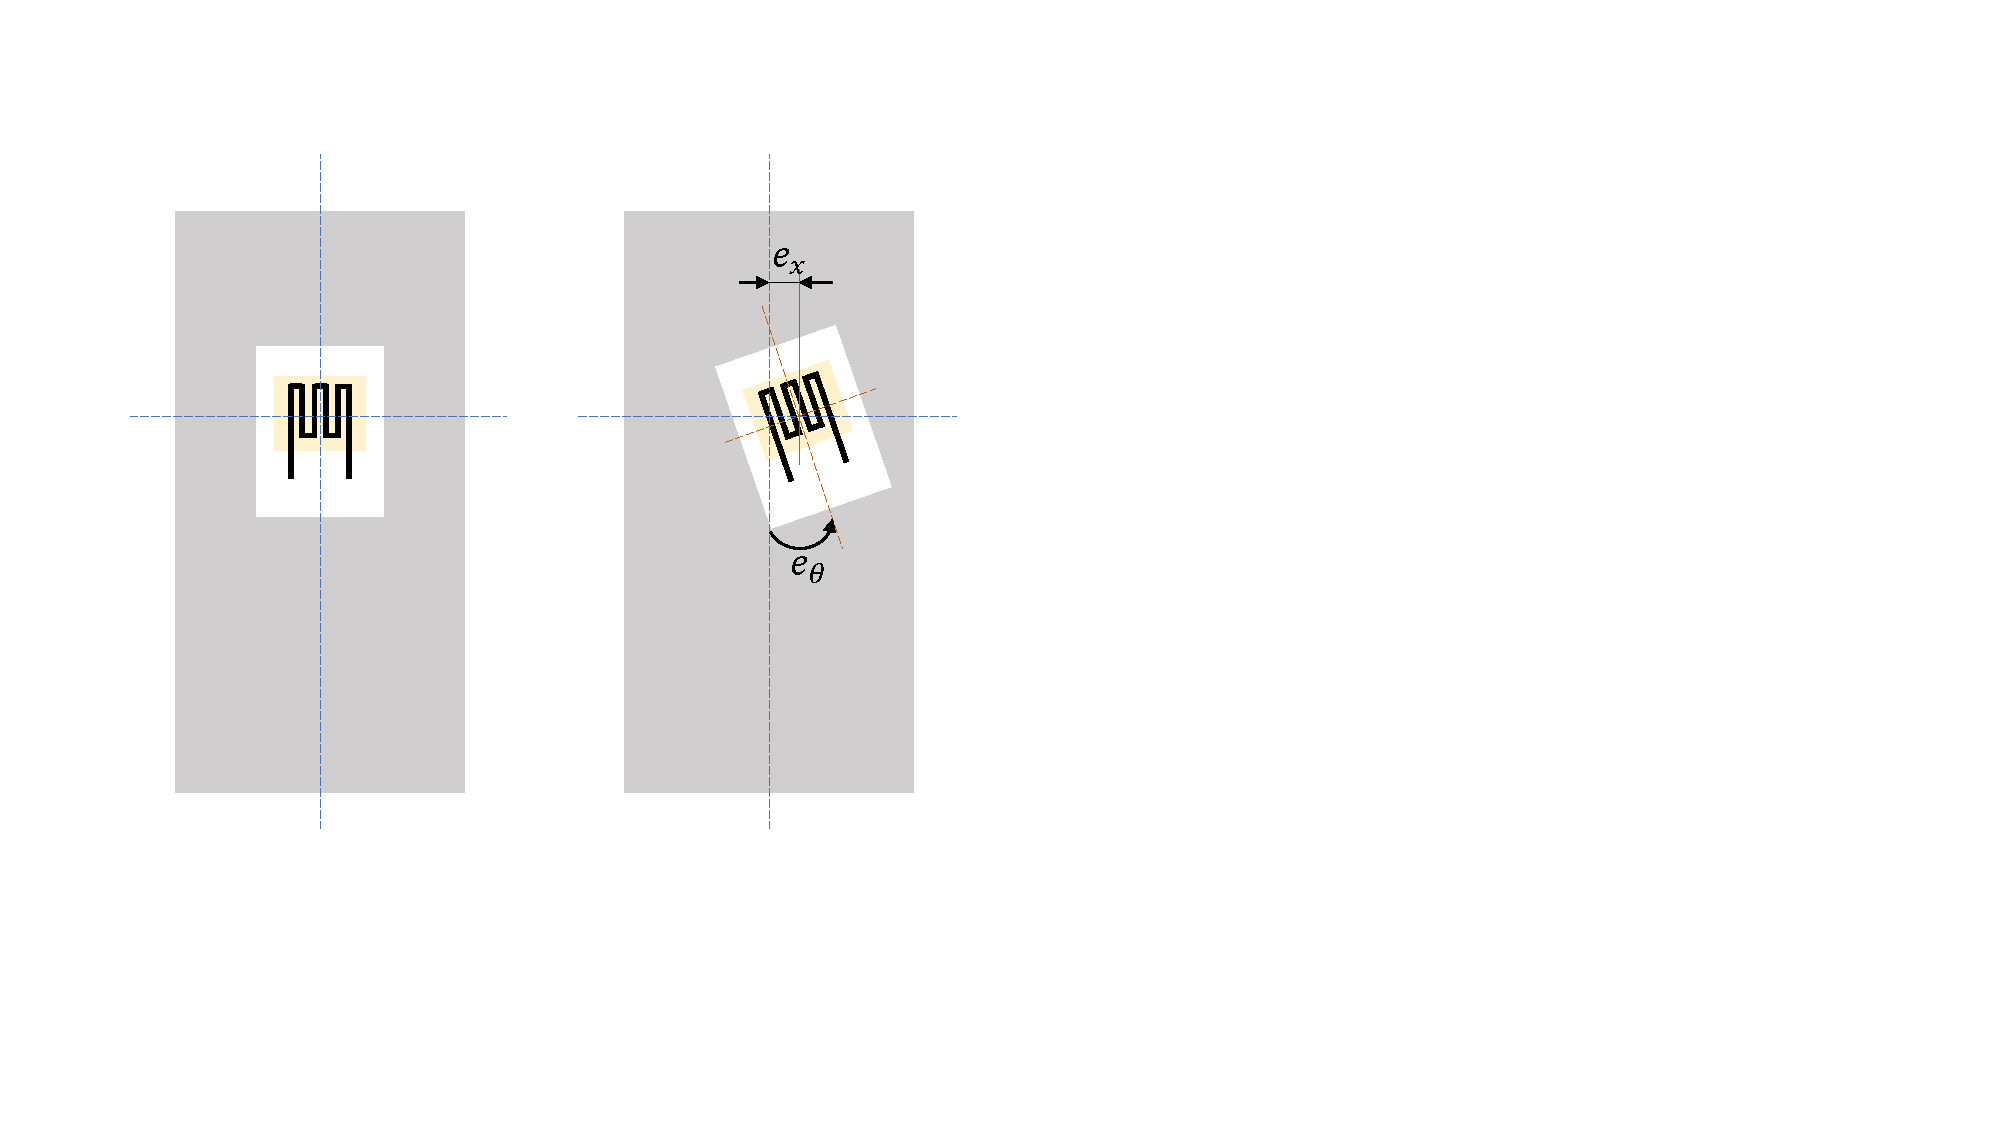
\includegraphics[height=0.35\columnwidth]{erroreMontaggioSensore} \label{fig:strainGaugeMisalignment}}
%	\subfigure[]{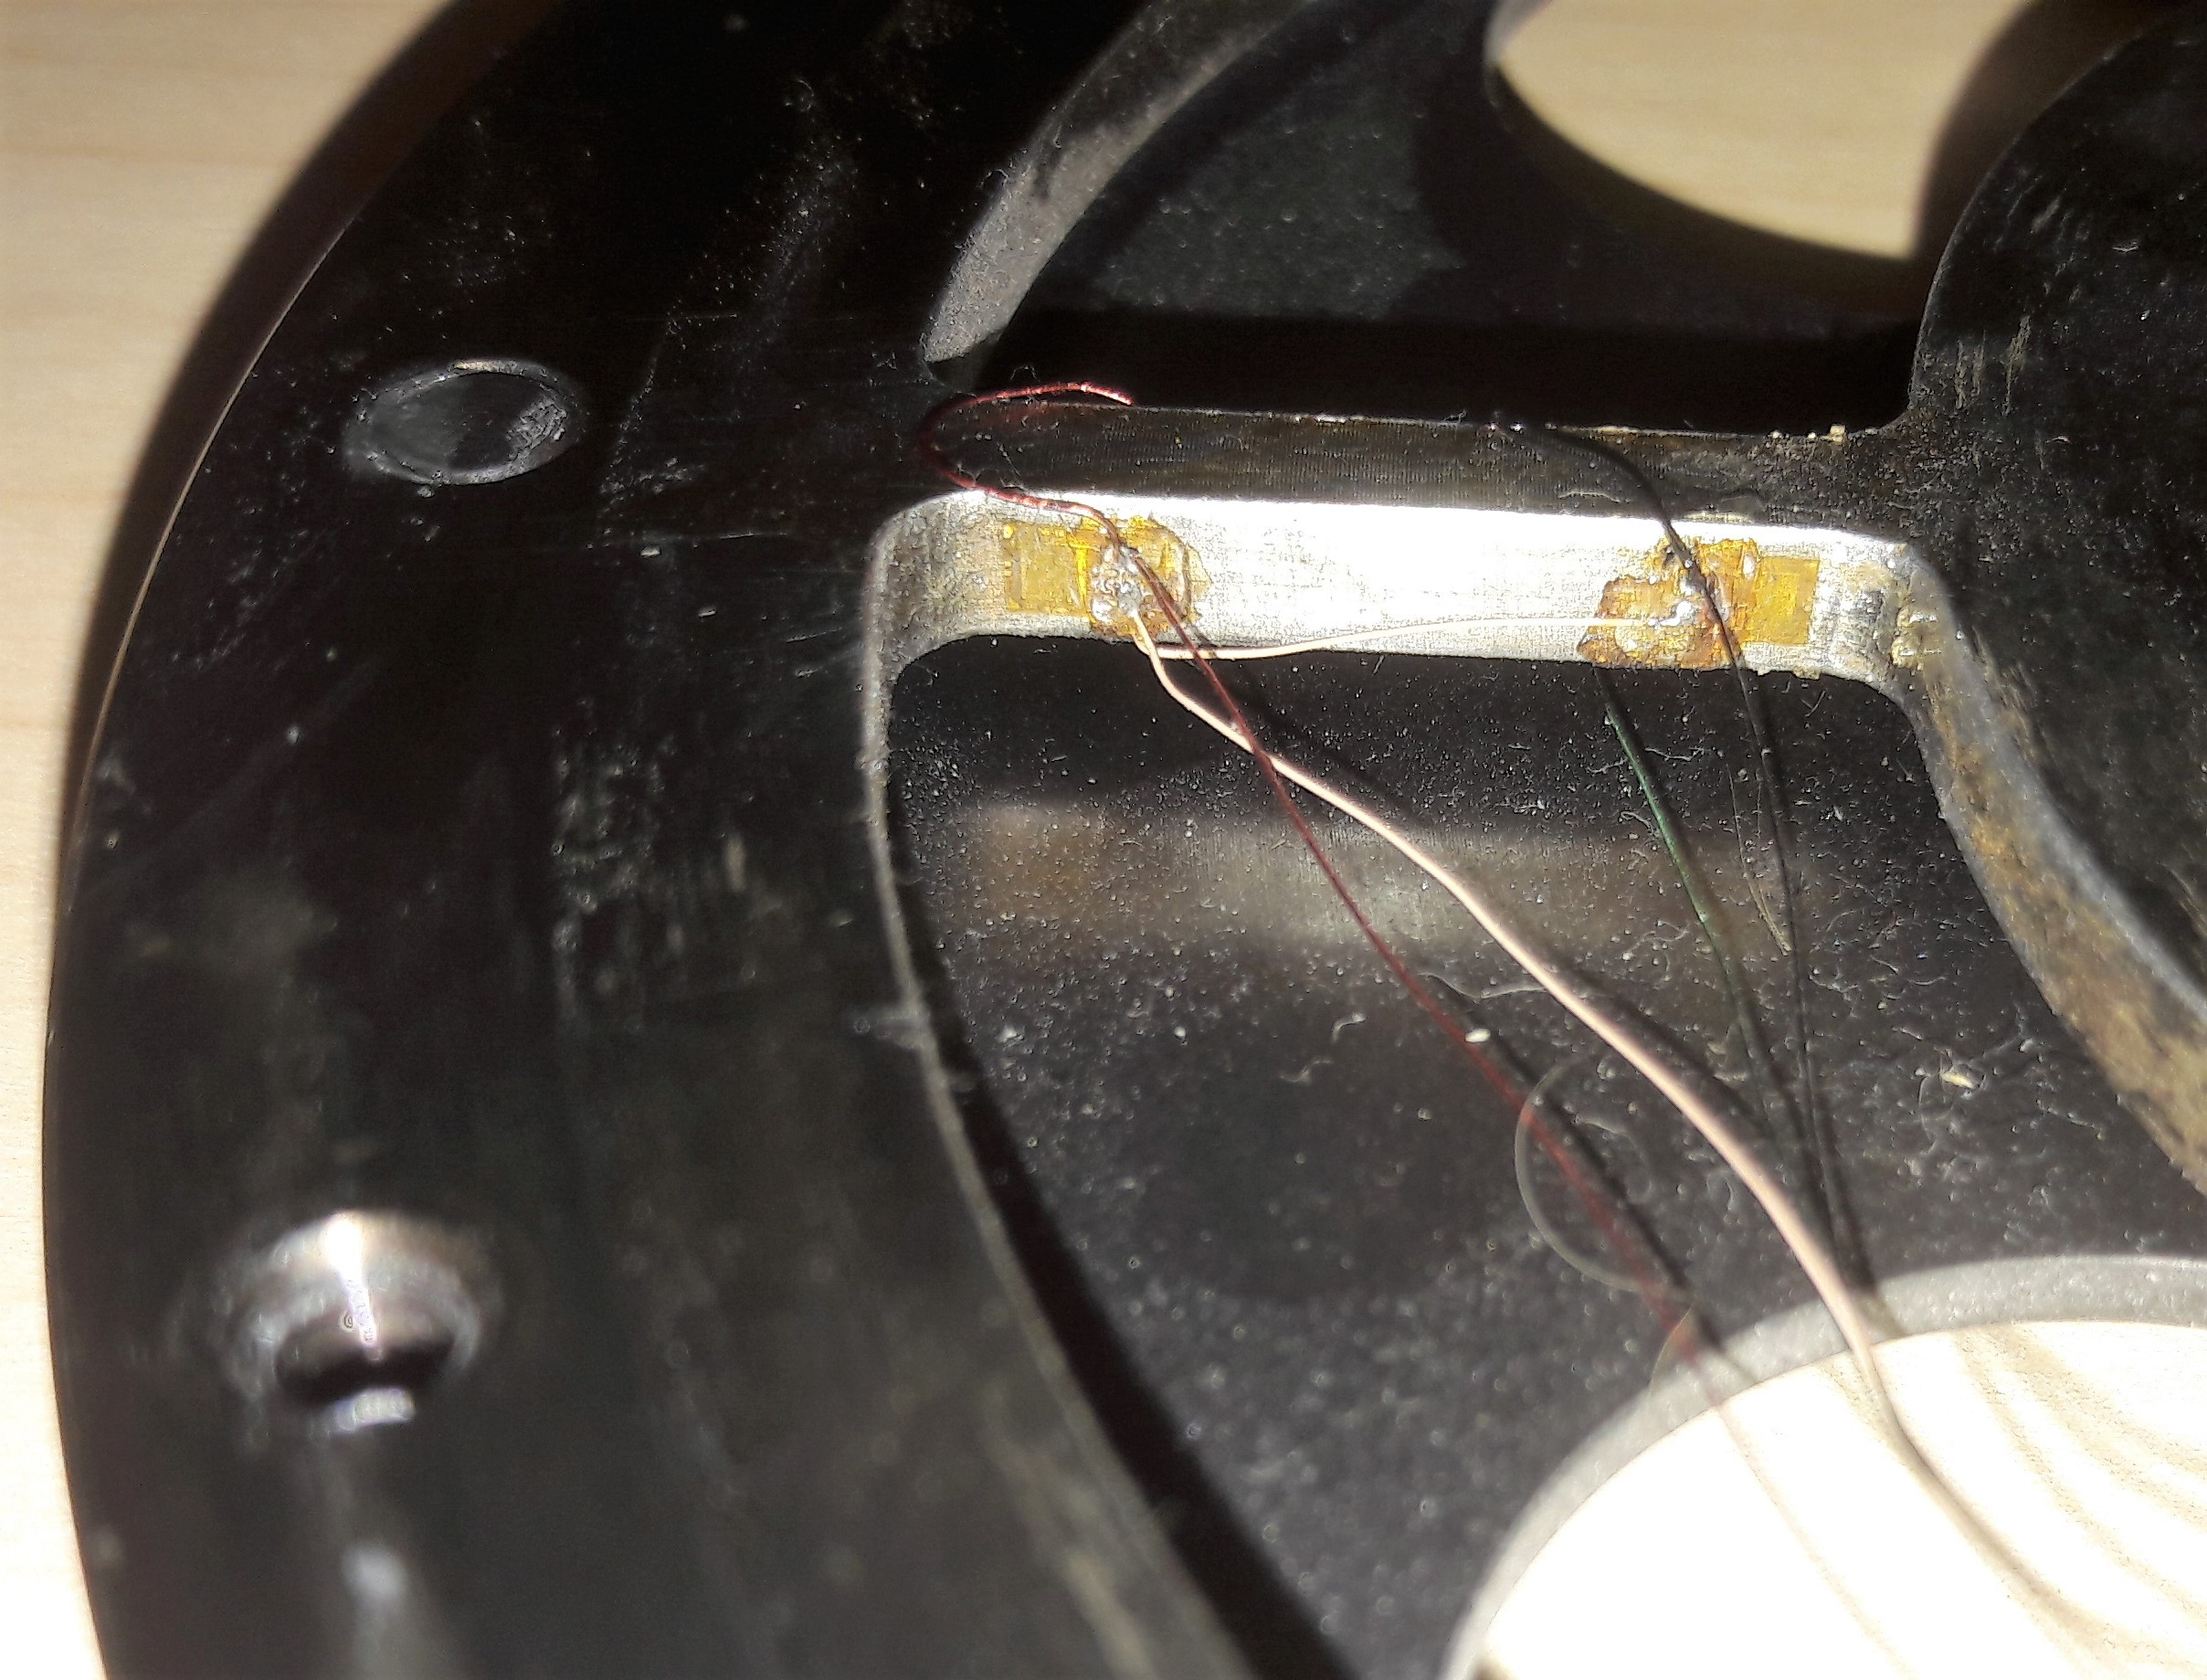
\includegraphics[height=0.32\columnwidth]{strainGaugeParticular.jpg} \label{fig:strainGaugeParticular}}
	\def\svgwidth{2\columnwidth}
	\begin{footnotesize}
		\input{imgRevised/fem_sensore.pdf_tex}
	\end{footnotesize}
	\caption{(a) A possible cause of high sensitivity to non-axial load is the strain gauges's mounting misalignment. $e_x$ is the linear displacement and the angular one is $e_{\theta}$ are highlighted. (b) A detail of the mounted strain gauges on the torque sensor. (c) For the FEM analysis a more dense grid mesh for the zone of interest has been used. For each area the average strain along the radial direction has been computed. (d) The FEM analysis results of the torque sensor, and of the flexible spline  deformation under non-axial load (e).}
	\label{fig:strainGaugeDeformation}
\end{figure*}

About the second hypothesis it is worth to notice that the sensor from a structural point of view is in series to the HD and these are in parallel with a couple of bearings. This parallel chain composes a hyper-static system (see \figurename \ \ref{fig:schemaGiuntoEMolle}), therefore the excessive sensitivity may be due to mounting misalignment of the mechanical parts of the chain. 
%
\begin{figure}[b]
	\centering
%	\subfigure[]{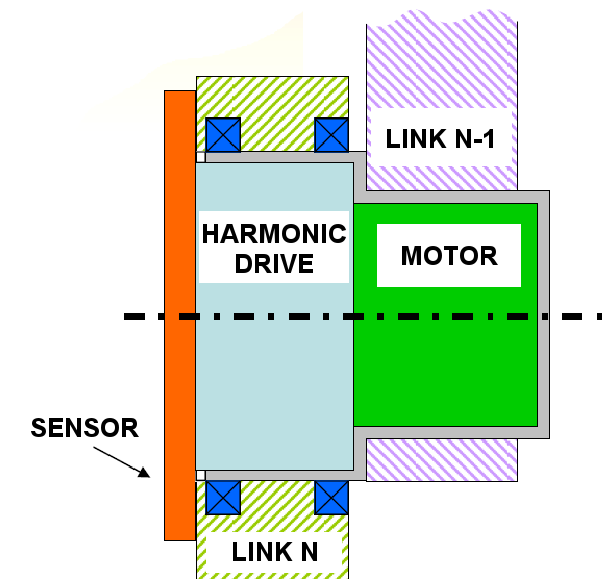
\includegraphics[width=0.49\columnwidth]{schemaGiuntoMod}\label{fig:schemaLinkGiuntoSens}}
%\subfigure[]{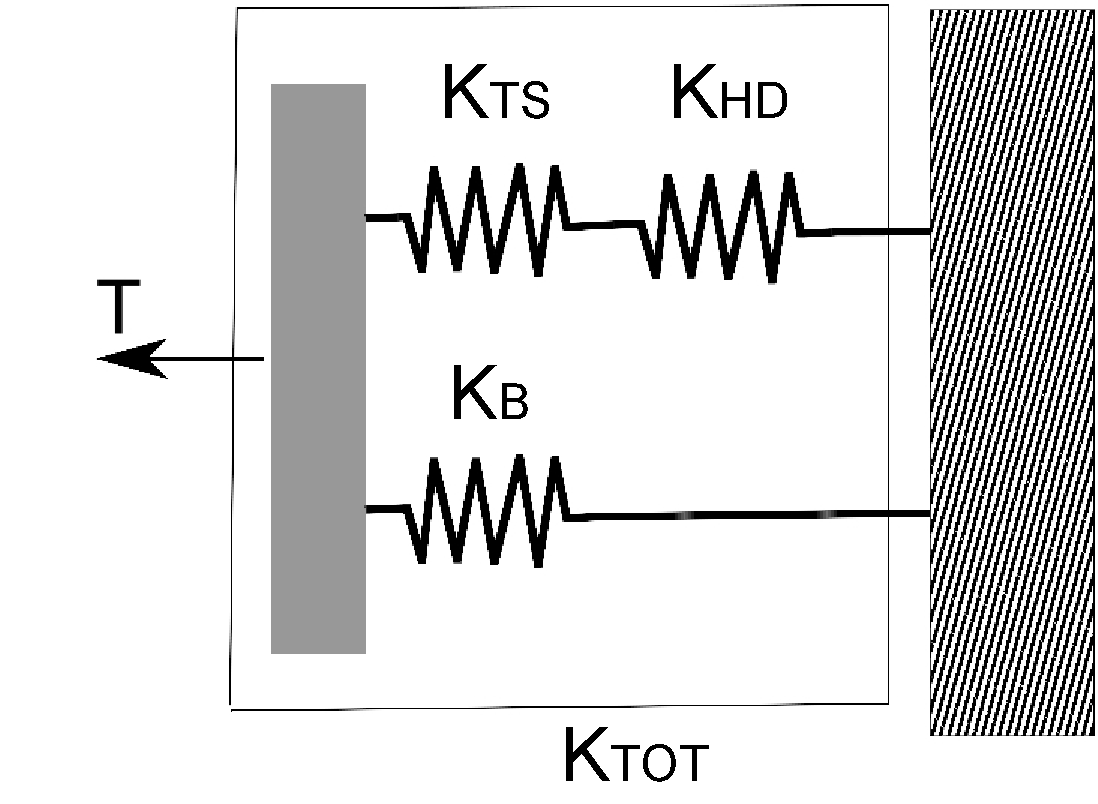
\includegraphics[width=0.49\columnwidth]{schemaMolle.pdf}\label{fig:schemaMolle}}
	\def\svgwidth{1\columnwidth}
	\begin{footnotesize}
		\input{imgRevised/Molle.pdf_tex}
	\end{footnotesize}
	\caption{(a) The schematic representation of the joint. The torque sensor is a series elastic element between the motor and the link n. The torque sensor is not structural and has been designed to transmit only axial torque. (b) The kinematic chain of the joint to non-axial loads. $K_{TS}$ and $K_{HD}$ are the stiffness of the torque sensor and of the Harmonic Drive to non-axial load respectively, whereas $K_B$ is the bearing stiffness.}
	\label{fig:schemaGiuntoEMolle}
\end{figure}
%
\par For the study of the hyper-static system a linear  elastic behavior of the system parts were supposed and the system response at non-axial moments was modeled as a mono-dimensional model. %% as in \figurename \ref{fig:schemaMolle}.
The overall joint stiffness to non-axial moments $K_{TOT}$ was experimentally evaluated, whereas the non-axial moment stiffness of the torque sensor $K_{TS}$ and of the HD $K_{HD}$ were computed via FEM analysis. The FEM results are depicted in \figurename \ \ref{fig:strainGaugeDeformation} and the stiffness values are reported in table \tablename \ \ref{tab:nonAxialStiffness}.
%
%\begin{figure}[]
%	\centering
%	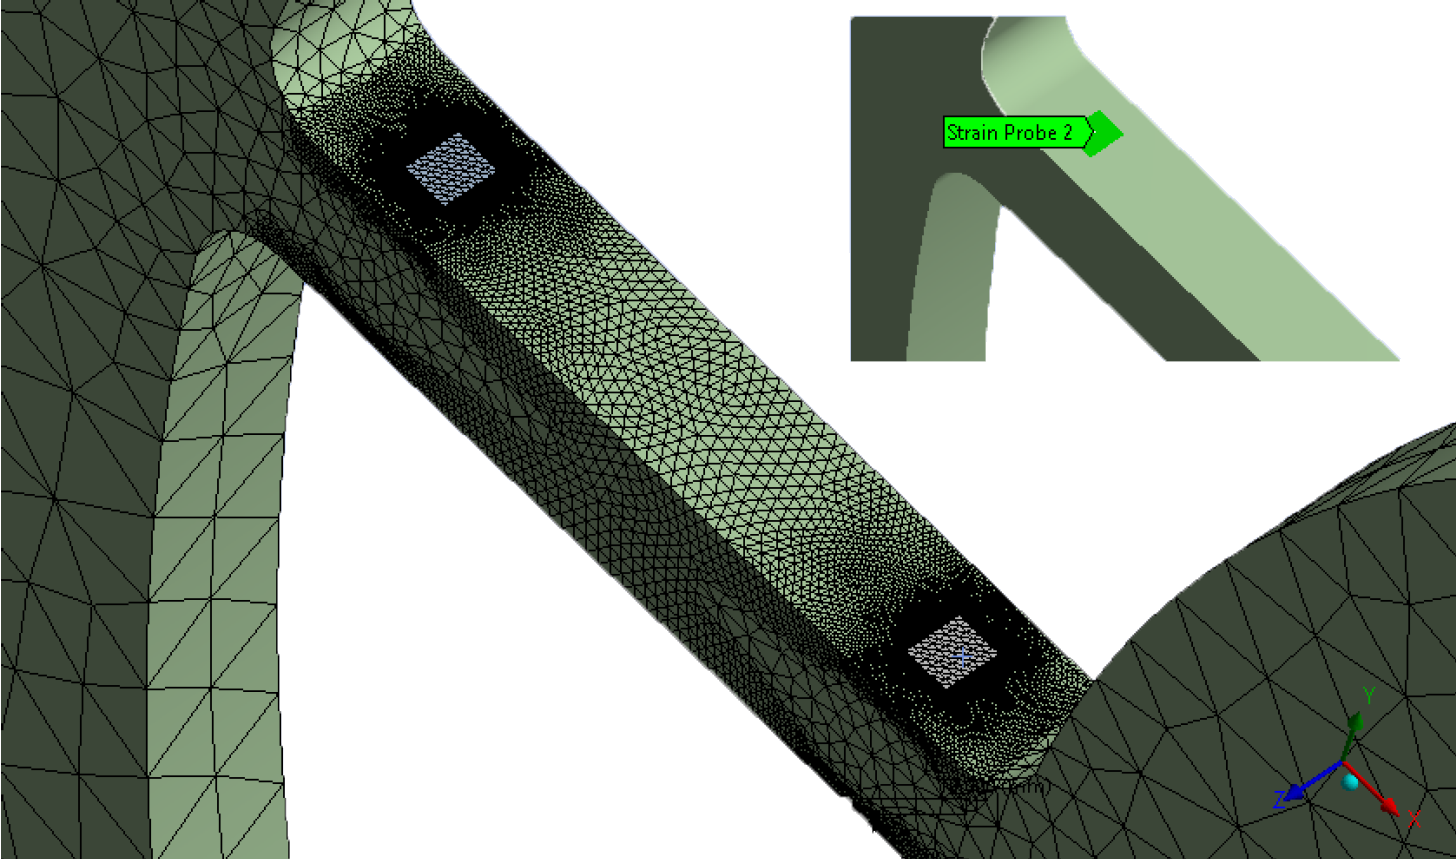
\includegraphics[width=0.7\columnwidth]{strainGaugeDeformation} 
%	\caption{For the FEM analysis a more dense grid mesh for the zone of interest has been used. For each area the average strain along the radial direction has been computed.}
%	\label{fig:strainGaugeDeformation}
%\end{figure}
%
\begin{table}[]
	\renewcommand{\arraystretch}{1.3}
	\caption{Stiffness of the components}
	\label{tab:nonAxialStiffness}
	\centering
	\begin{tabular}{c c}
		\hline \hline
		\bfseries Component & \bfseries Stiffness [kNm/rad]\\
		\hline
		$K_{TS}$  & 4.1\\
		$K_{HD}$  & 0.4\\
		$K_{B}$   & 23.6\\
		\hline
		$K_{TOT}$   & 24\\
		\hline \hline
	\end{tabular}
\end{table}
%
%
\par A possible mounting misalignment of the hyper-static chain may be a collinear and/or concentric mounting misalignment between the sensor axis and the bearing axis. In this case, the HD works as an universal joint that connect the sensor (that is connected to the n+1 link ) and the n-th link. The sensitivity to non-axial moments defined in equation \eqref{eq:sensitivityToNonAxLoad} and  the mechanical properties  in \tablename \ \ref{tab:nonAxialStiffness} lead to a theoretical mounting misalignment of about $0.5 \ mm$, but this value is not in agreement with the design tolerances and components data-sheets from which a misalignment of about $0.05 \ mm$ results in the worst case.
%
%The internal joint-torque sensor introduces controlled torsional compliance that is used at the same time to transmit joint torque actuation  from the motor to the link and to measure it. 
%The torque sensor is not structural and the mechanical transmission is parallel (see the scheme in \figurename \ \ref{fig:schemaLinkGiuntoSens}). The planar sprocket hub has been designed to be sensitive only to the torque along the motor axes exchanged between the motor on the link $n-1$ and the link $n$, while theoretically the torques along the other two axes are transmitted directly through the ball bearings between the link $n-1$ and the link $n$.
\par To summarize, unwanted sensor reads to non-axial load may be due to the combination of effects from sensor mounting misalignments and HD excessive deformation. 
\par In order to minimize this undesired effect, we adopted a  model-free adaptive method based on artificial neural networks (ANN) to characterize and compensate this non-linear response of the sensors, in alternative to modeling approaches in reason of the complexity of the phenomenon. 
% that might be difficult to model.
%
%
Considering the ideal and linear response of the sensor, the torque readings can be expressed as $\tau_s = k_v * v$, where $v$ is the measured voltage tension and $k_v$ is the torque sensor's voltage constant. In the real case it can be written $\hat{\tau}_s = k_v \cdot v + \delta\tau$, where $\delta\tau$ is the non-linear influence on the sensor readings due to the mounting and non-axial loads.
By experimental evidence, it's possible to assert that the term $\delta\tau$ varies in a non-linear way with respect to the exoskeleton pose (joint angles) and load.
\par The mounting errors influence the torque readings non-linearly with respect to the joint angle, while the non-axial torques depend in part on the interaction with the human and in part on the dynamics and gravitational torques acting on the considered joint.
%\begin{figure}[htb]
%	\centering
%	\includegraphics[width=0.55\columnwidth]{\figpath{schemaGiuntoMod}}	
%	\caption{}
%	\label{fig:schemaLinkGiuntoSens}
%\end{figure}
%
%\begin{figure}[]
%	\centering
%	\subfigure[]{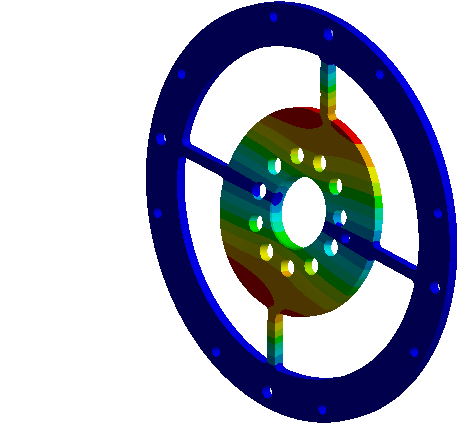
\includegraphics[height=0.4\columnwidth]{sensoreCarichiSpuri} \label{fig:sensoreCarichiSpuri}	}
%	\subfigure[]{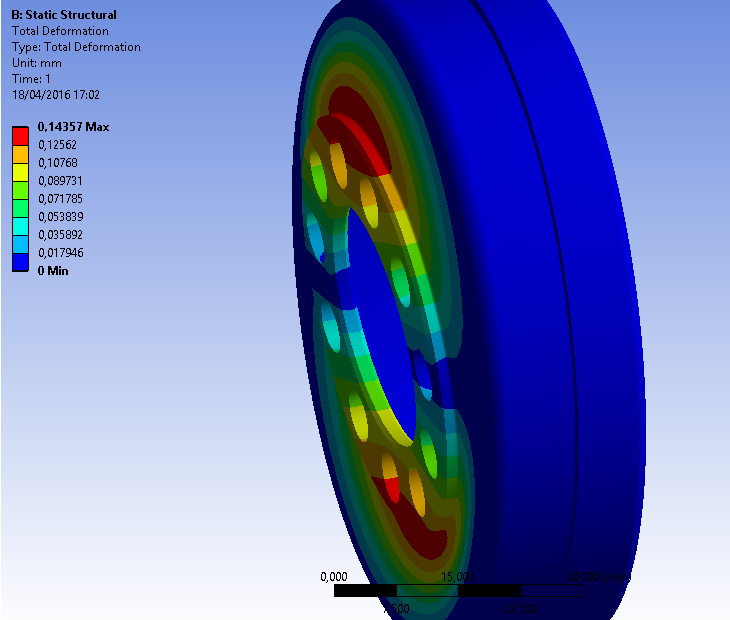
\includegraphics[height=0.4\columnwidth]{HDCarichiSpuri} \label{fig:HDCarichiSpuri} }
%	\caption{The FEM analysis results of the torque sensor (a) and of the flexible spline (b) deformation under non-axial load.}
%\end{figure}
%
%
For all three sensors, the $k_v$ constants have been experimentally evaluated. In order to minimize the effect of non-linear undesired term $\delta\tau$,  an ANN has been used. An ANN is a mathematical approximation approach that can infer non-linear behavior from experimental acquisitions. The ANN with 7 neurons in the hidden layer and sigmoid activation function are employed to estimate the error on the basis of the 4 angles and load on each axis. The angular information is useful to infer the assembly error component, whereas for the load influence the gravitational torque has been used. 
\par To train the neural network the whole workspace has been partitioned in 414 target points. The torque sensor readings were acquired while the exoskeleton was holding the target position. For each joint, the training has been done using as input the 4 angles and the gravity torque that act on the joint (computed by model), and as output the residual value $\hat{\delta\tau} = G_i(\vect{\theta_m}) - k_v * v$, where $G_i$ is the gravity load on the i-th joint when the pose is given by the angle vector $\vect{\theta_m}$. The set of target points was divided in 3 parts: 70\% for the training set, 20\% for the validation set and 10\% for the test set. The regression value between the ANN output and the target points is 0.99.
The actual sensor torque estimation is given by $\bar{\tau}_s = k_v * v + \delta\tau(\vect{\theta_m},G_i)$.%, and a scheme of this estimation is shown in the \figurename \ \ref{fig:NN_schema}.
%\begin{figure}[]
%	\centering
%	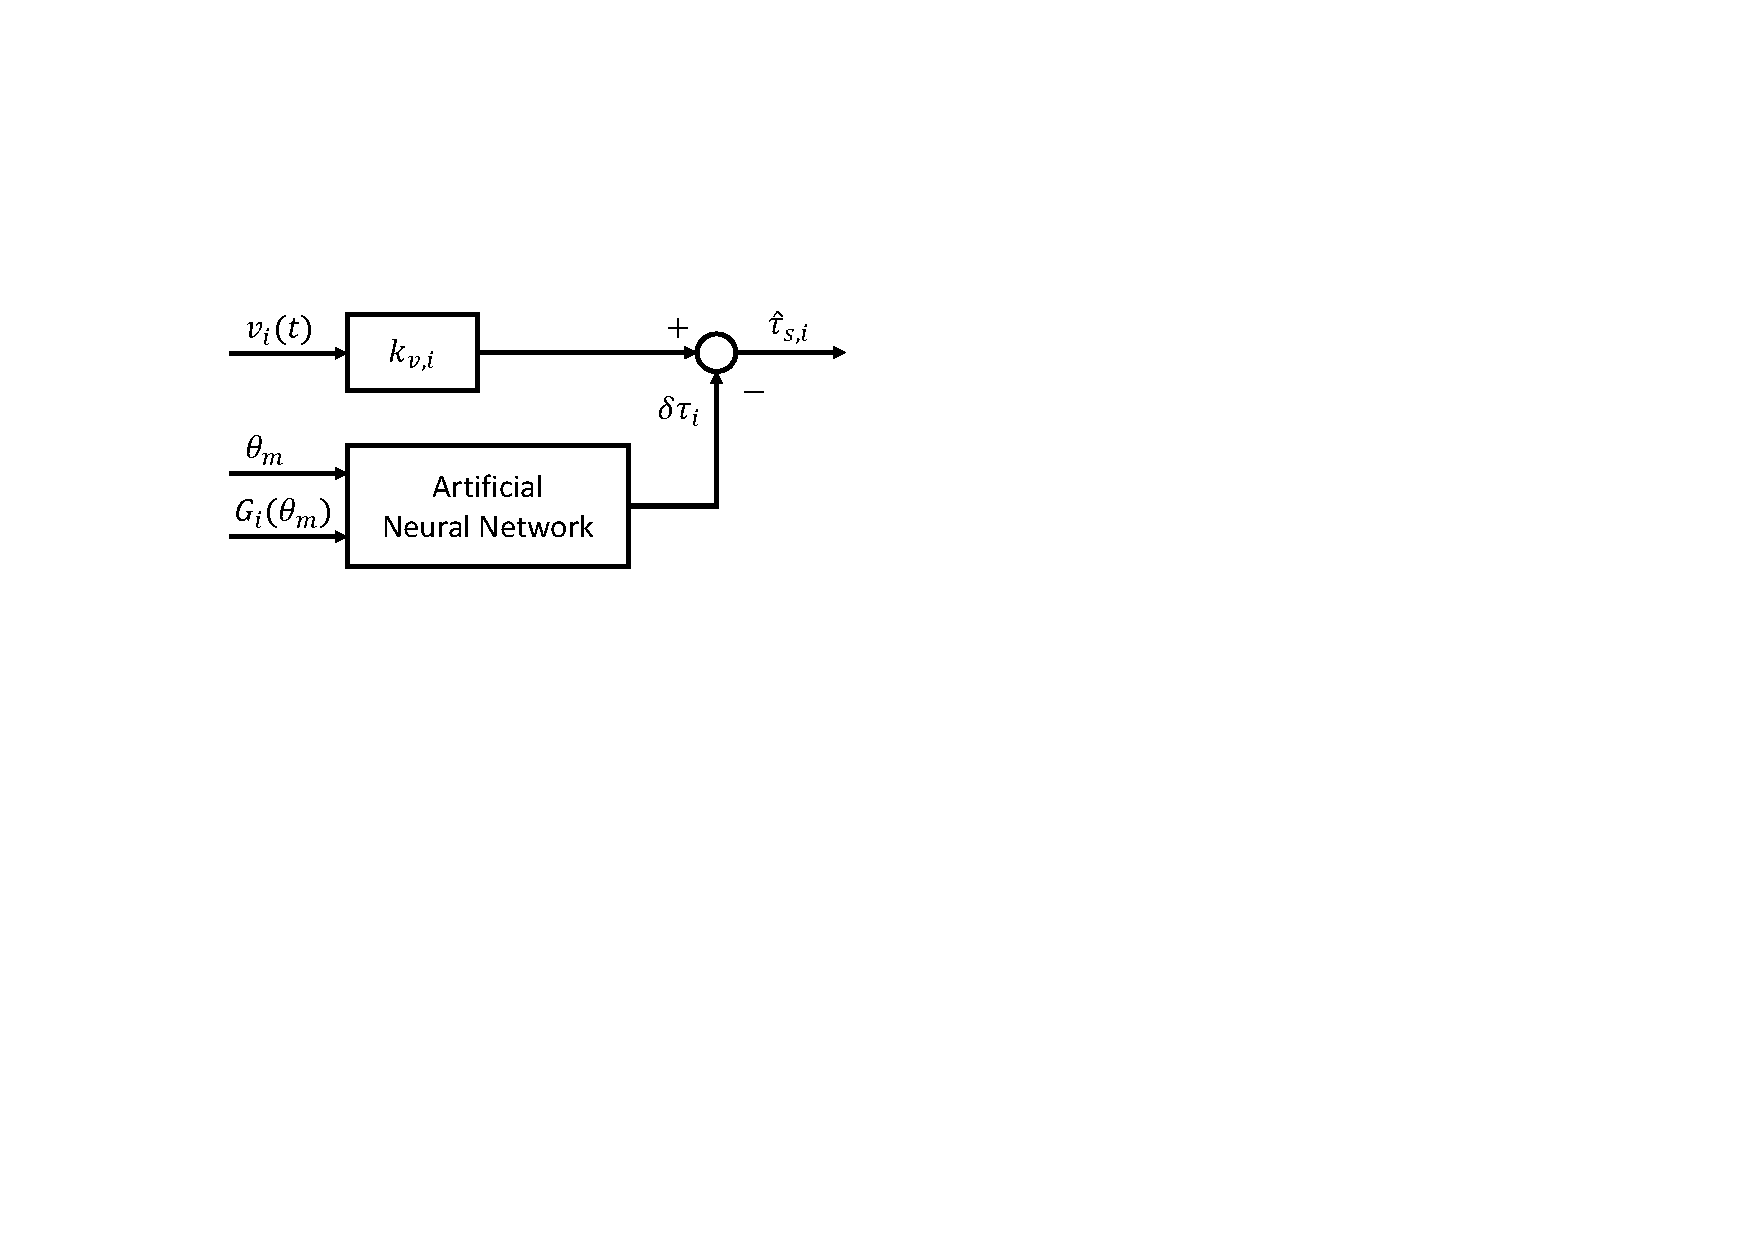
\includegraphics[width=0.7\columnwidth]{torqueEstimation}	
%	\caption{The estimated sensor torque is obtained as the sum of sensor's reading and the predicted undesired non-linear term.}
%	\label{fig:NN_schema}
%\end{figure}
%\hl{QUi} As can be shown in the \figurename \ N, the introduction of the undesired term prediction induce a reduction in interaction force while a zero torque following control is implemented (see section N). Note that the force reduction is measured by the end effector force/torque sensor, while the  torque control use only the estimated torque using the sensor readings.
%%%%%%%%%%%%%%%%%%%%%%%%%%%%%%%%%%%%%%%%%%%%%%%%%%%%%%%%%%%%%%%%%%%%%%%%%%%%%%%%%%%%%%%%%%%%%%%%%%%%%%%%%%%%%%%%%%%%
%%%%%%%%%%%%%%%%%%%%%%%%%%%%%%%%%%%%%%%%%%%%%%%%%%%%%%%%%%%%%%%%%%%%%%%%%%%%%%%%%%%%%%%%%%%%%%%%%%%%%%%%%%%%%%%%%%%
\subsection{Control Hardware}
%\hldone{Done}
The control architecture of the Rehab-Exos is decentralized and based on the EtherCAT communication bus in order to guarantee both optimal signal to noise ratio in the acquisition of analogical signals, i.e. force sensors, and higher standards of safety.
The EtherCAT communication network consists of one master controller and four Ethercat Slave Controllers (ESC), one for each actuation joint.
The master controller is handled by Simulink Real-Time\texttrademark \ Operating System that executes the centralized control model at $2 \ kHz$ frequency.

Motors of the exoskeleton consist of three $170 \ VDC$ power supplied brushless motors on the 1st, 2nd, and 4th joint each one driven by programmable current drivers and one $48 \ VDC$ power supplied DC motor on the 3rd joint.  All of them are provided with one incremental encoder and one torque sensor.

Each ESC board is a custom control board featuring an up to $72 \ Mhz$ ARM7 micro-controller, 4 14-bit DAC output interfaces (to set the reference of the current drives), 10 14-bit Analog-to-Digital Converter (ADC) channels (to acquire the torque signals through 2 Wheatstone full-bridge channels that are pre-amplified) and the EtherCAT ET1100 controller linking to double-port Ethernet interface.
%\begin{figure}[ht]
%	\centering
%	{\includegraphics[width=0.95\columnwidth]{\figpath{HWControlDiagram}}}
%	\caption{The decentralized control architecture}
%	\label{fig:ControlArchitecture}
%\end{figure}
\section{Dynamic model} \label{sec:dynamic_model}

\subsection{Single joint model} \label{Single joint model}
%\hldone{DONE}
The joints of the exoskeleton can be modeled with a lumped parameter model due to the elasticity of the harmonic drive speed reducer and torque sensor (for joints 1, 2 and 4) and of tendon transmission for joint 3. The used single joint model is a 2-mass with spring and damper (Fig. \ref{fig:exos_singlejoint_model}).

\par The single joint dynamics is formulated by the following equations:

\setlength{\arraycolsep}{0.0em}
\footnotesize
\begin{align}
%\label{eqn:dinamicaMotoreSingoloGiunto}
I_{m,i} \ddot{\theta}_{m,i}  + c_{m,i}\dot{\theta}_{m,i} + c_{t,i} (\dot{\theta}_{m,i}-\dot{\theta}_{i})  
{+}\:k_{t,i} ({\theta_{m,i}}-{\theta_i}) &= \tau_{m,i}+\tau_ {d,i} \nonumber	\\
\label{eqn:dinamicaLinkSingoloGiunto}
I_{l,i} \ddot{\theta}_{i}+c_{t,i} (\dot{\theta}_{i}-\dot{\theta}_{m,i})
+k_{t,i} ({\theta_{i}}-{\theta_{m,i}}) &= \tau_{l,i}	
\end{align}
\normalsize
\setlength{\arraycolsep}{5pt}

where referring to the i-th joint, $\theta_ {m,i}$ and $\theta_ {i}$ stand for motor and joint angles respectively, $k_{t,i}$ and $c_{t,i}$ are the stiffness and viscous coefficient of the transmission, that were experimentally characterized.
$I_{m,i}$ is motor inertia, $I_{l,i}$ is average link inertia considered as constant, $\tau_{m,i}$ is the motor torque, $\tau_{d,i}$ is a disturbance torque acting on the motor rotor  which accounts for internal friction and ripple effects of both motor and harmonic drive, while $\tau_{l,i}$ is the external torque acting directly on the output link. The $\tau_{l,i}$ torque accounts for the 
exogenous input due to the interaction  with the human, and endogenous input accounting for unmodeled non-linear effects, such as dynamic or gravity forces.
\begin{figure}[ht]
	\centering
	%{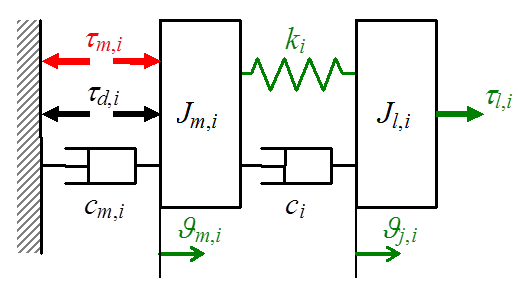
\includegraphics[width=0.5\columnwidth]{2massModel}}
	\def\svgwidth{0.7\columnwidth}
	\begin{footnotesize}
		\input{imgRevised/2MassModel.pdf_tex}
	\end{footnotesize}
	\caption{The 2-mass model for each joint.}
	\label{fig:exos_singlejoint_model}
\end{figure}
%%%%%%%%%%%%%%%%%%%%%%%%%%%%%%%%%%%%%%%%%%%%%%%%%%%%%%%%%%%%%%%%%%%%%%%%%%%%%%%%%%%%%%%%%%%%%%%%%%%%%%%%%%%%%%%%%%%%
%%%%%%%%%%%%%%%%%%%%%%%%%%%%%%%%%%%%%%%%%%%%%%%%%%%%%%%%%%%%%%%%%%%%%%%%%%%%%%%%%%%%%%%%%%%%%%%%%%%%%%%%%%%%%%%%%%%%
\subsubsection{Experimental characterization of single joint performance}
%\hldone{DONE}
%\point{Insert here experimental data and procedures with indication of dynamic bandwidth}
As described in \ref{subsec:mechanicalDesign} the joint is equipped with a torque sensor that is a part of the transmission chain and is capable of measuring the elastic torque $\tau_{s,i}$, which acts between motor rotor and joint output link. The elastic sensor torque can be expressed by $\tau_{s,i} = k_{t,i} (\theta_{i}-\theta_{m,i})$. The joint dynamics can be re-written expliciting the $\tau_{s,i}$ readings starting from  $\tau_{s,i}$ definition, its 1st and 2nd derivatives and using the equations  \ref{eqn:dinamicaLinkSingoloGiunto}. It is obtained:
\begin{equation}
\label{eqn:dinamicaSensoreCoppia}
\ddot{\tau}_{s,i} + \frac{c_{t,i}}{I_i}\dot{\tau}_{s,i} + \frac{k_{t,i}}{I_i}\tau_{s,i}= \frac{k_{t,i}}{I_{l,i}}\tau_l + \frac{k_{t,i}}{I_{l,i}}\tau_g - \frac{k_{t,i}}{I_{m,i}}\tau_d - \frac{k_{t,i}}{I_{m,i}}\tau_m
\end{equation}
where $I_i = I_l I_m /(I_l+I_m)$. The natural frequency of this system is $\omega_n = \sqrt{k_{t,i} /I_i } /2\pi$. The natural frequency has been experimentally evaluated for a single joint in a test-rig analyzing the response of the $\tau_s$ when a chirp command is used for the $\tau_m$ motor torque. 
\par From Fig. \ref{fig:OpenLoopJointBode}, use of the Half-Power Bandwidth method returns $c = 11.8 \, \text{Nms/rad}$ as the overall damping coefficient of the flexible joint (this value has also been validated via the Logarithmic Decrement method).
\begin{figure}[ht]
	\centering
%	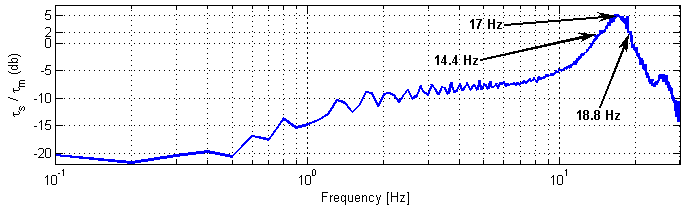
\includegraphics[width=1\columnwidth]{OpenLoopJointBode}
	\def\svgwidth{1\columnwidth}
	\begin{footnotesize}
		\input{imgRevised/bode_rehab_joint.pdf_tex}
	\end{footnotesize}
	\caption{Experimental open-loop response (Bode magnitude plot) of joints 1,2 and 4: joint sensor torque vs. motor torque command in standardized testbed conditions.}
	\label{fig:OpenLoopJointBode}
\end{figure}
Considering the exoskeleton, every joint sees a link inertia that depends on the pose so the natural frequency of each joint depends on the pose of the exoskeleton. 
Considering an average link inertia, it can be obtained the natural frequency for each joint elastic transmission. Results are shown in the \tablename \ \ref{tab:naturalFrequencies}.
%\begin{table}[!t]
%	\renewcommand{\arraystretch}{1.3}
%	\caption{The natural frequency of the joints}
%	\label{tab:naturalFrequencies}
%	\centering
%	\begin{tabular}{|c|c|c|}
%		\hline
%		\bfseries Joint & \bfseries Avg. link inertia [$Kg/m^2$] & \bfseries Natural freq. [$Hz$]\\
%		\hline\hline
%		1 & 0.9639 & 19.3930\\
%		\hline
%		2 & 1.11 & 18.3501\\
%		\hline
%		4 & 0.1925 & 39.6797\\
%		\hline
%	\end{tabular}
%\end{table}
\begin{table}[!t]
	\renewcommand{\arraystretch}{1.3}
	\caption{The natural frequency of the joints}
	\label{tab:naturalFrequencies}
	\centering
	\begin{tabular}{c c c}
		\hline \hline
		\bfseries Joint & \bfseries Avg. link inertia [$Kg/m^2$] & \bfseries Natural freq. [$Hz$]\\
		\hline
		1 & 0.9639 & 19.3930\\
		2 & 1.11 & 18.3501\\
		4 & 0.1925 & 39.6797\\
		\hline \hline
	\end{tabular}
\end{table}
For all these three joints the motor inertia is the same and it is equivalent to $3.742 \, \text{ Kg/m}^2$.


%%%%%%%%%%%%%%%%%%%%%%%%%%%%%%%%%%%%%%%%%%%%%%%%%%%%%%%%%%%%%%%%%%%%%%%%%%%%%%%%%%%%%%%%%%%%%%%%%%%%%%%%%%%%%%%%%%%%
%%%%%%%%%%%%%%%%%%%%%%%%%%%%%%%%%%%%%%%%%%%%%%%%%%%%%%%%%%%%%%%%%%%%%%%%%%%%%%%%%%%%%%%%%%%%%%%%%%%%%%%%%%%%%%%%%%%%
%%%%%%%%%%%%%%%%%%%%%%%%%%%%%%%%%%%%%%%%%%%%%%%%%%%%%%%%%%%%%%%%%%%%%%%%%%%%%%%%%%%%%%%%%%%%%%%%%%%%%%%%%%%%%%%%%%%%
%%%%%%%%%%%%%%%%%%%%%%%%%%%%%%%%%%%%%%%%%%%%%%%%%%%%%%%%%%%%%%%%%%%%%%%%%%%%%%%%%%%%%%%%%%%%%%%%%%%%%%%%%%%%%%%%%%%%
\subsection{Multiple joints model} \label{Full dynamics model}

Given the single joint two-mass model, the dynamic model of the whole exoskeleton can be formulated in matrix form as follows:
\setlength{\arraycolsep}{0.0em}


%\footnotesize

\begin{equation}
%\left \{
\begin{IEEEeqnarraybox}[][c]{l}
\overbrace{\colorboxed{red}{\vectm{I_m}    \vectm{D} \vects{\ddot{\uptheta}_m} + \vectm{B_m } \vectm{D} \vects{\dot{\uptheta}_m} }}^{\text{Motor Dynamics}}
 +
  \overbrace{  \colorboxed{green}{\vectm{C_t}  ( \vectm{D} \vects{\dot{\uptheta}_m} - \vects{\dot{\uptheta}} )+ 
  		\:\vectm{K_t}  ( \vectm{D} \vects{\uptheta_m}- \vects{\uptheta} ) }}^{\text{Elastic transmission torque}}
  =  \\ \vects{\uptau_m} +\vects{\uptau_d}   \\
\underbrace{\colorboxed{red}{\vectm{M}(\vects{\uptheta}) \vects{\ddot{\uptheta}}  + \vectm{C}( \vects{\dot{\uptheta}}, \vects{\uptheta})   \vects{\dot{\uptheta}}}}_{\text{Joint dynamics}}
 +   
 %\underbrace{  \colorboxed{green}{ }}_{\text{Joint dynamics}}
\underbrace{  \colorboxed{green}{
 \vectm{C_t}  ( \vects{\dot{\uptheta}} - \vectm{D} \vects{ \dot{\uptheta}_m} )
{+}\: \vectm{K_t}  ( \vects{\uptheta} - \vectm{D}\vects{\uptheta_m} )}}_{\text{Elastic transmission torque}} + \\ + \vect{G}( \vects{\uptheta}) = \vectm{J^T} \vect{F_h}
\label{eqn:dinamicaLinkMultiGiunto}
\end{IEEEeqnarraybox}
%\right . %\label{eqn:dinamicaMotoreMultiGiunto}
\end{equation}
%\label{eqn:dinamicaMotoreMultiGiunto} 
\normalsize
\setlength{\arraycolsep}{5pt}
%
%\fbox{$\displaystyle
%	\smash{\callout{F}{\stackunder{$1,n$}{we only consider 1 unknown}}} = 
%	\left[
%	\frac{\partial f}{\partial l_1}\quad
%	\frac{\partial f}{\partial l_2}\quad
%	\frac{\partial f}{\partial l_3}
%	\cdots
%	\frac{\partial f}{\partial l_n}
%	\right]
%	$}
%
%\vspace{2 cm }

%\begin{eqnarray}
%\label{eqn:dinamicaMotoreMultiGiunto}
%\vectm{J_m}    \vectm{D} \vects{\ddot{\theta}_m} + \vectm{B_m  D} \vects{\dot{\theta}_m}  + \vectm{C_t}  ( \vectm{D} \vects{\dot{\theta}_m} - \vects{\dot{\theta}_j} )+ 
%\:\vectm{K_t}  ( \vectm{D} \vects{\theta_m}- \vects{\theta_j} ) =  \nonumber\\ \vects{\tau_m} +\vects{\tau_d}
%\end{eqnarray}


%\begin{eqnarray}
%\label{eqn:dinamicaLinkMultiGiunto}
%\vectm{M}(\vects{\theta_j}) \vects{\ddot{\theta}_j}  + \vectm{C}( \vects{\dot{\theta}_j}, \vects{\theta_j})   \vects{\dot{\theta}_j} +   \vectm{C_t}  ( \vects{\dot{\theta}_j} - \vectm{D} \vects{ \dot{\theta}_m} )+ 
%{+}\: \vectm{K_t}  ( \vects{\theta_j} - \vectm{D}\vects{\theta_m} ) + \nonumber\\ + \vects{G}( \vects{\theta_j}) = \vectm{J}^T \vects{F_h}
%\end{eqnarray}


%where $\vectm{D}$ is a diagonal matrix modeling the reduction factor introduced by joint speed reducers, $\vectm{J_m}$ and $\vectm{B_m}$ are diagonal matrices modeling inertia and viscous friction at motor respectively; $\vectm{K_t}$ and $\vectm{C_t}$ are diagonal matrices modeling stiffness and damping associated to the elastic transmission; $\vects{G}$ models the effects of gravity force on links.
where $\vectm{I_m}$, $\vectm{B_m}$, $\vectm{D}$, $\vectm{K_t}$ and $\vectm{C_t}$ are diagonal matrices.  $\vectm{I_m}$ and $\vectm{B_m}$ model inertia and viscous friction at motor respectively, while $\vectm{K_t}$ and $\vectm{C_t}$ model stiffness and damping associated with the elastic transmission and $\vectm{D}$ models  the transmission reduction factor introduced by joint gearheads; $\vect{G}$ models the effects of gravity force on links;
$\vect{F_h}$ are the external  forces  acting on the system  due to human interaction  and the respective joint torques are computed by multiplying them by the transposed Jacobian matrix  $\vectm{J^T}$ evaluated in the actual exoskeleton configuration. The multi-joint model introduces cross-coupling among joints and non-linearities, with terms $ \vectm{C}( \vects{\dot{\uptheta}}, \vects{\uptheta})  $ that models Coriolis effects and $\vectm{M}(\vects{\uptheta}) $ that represents link inertias and that can be decomposed
into a diagonal constant component and a variable component as follows:

%By taking into account that
%that the real dynamics has terms  $\vectm{M}(\vects{\uptheta}) $  and $ \vectm{C}( \vects{\dot{\uptheta}}, \vects{\uptheta}) $ depending on the actual joint configuration, the first term can be decoupled into a diagonal constant component and a variable component as follows:
\begin{equation}
\vectm{M }  \vects{\ddot{\uptheta}}=
\underbrace{\overline{\vectm{M} } \vects{\ddot{\uptheta}}}_{\text{constant}}
 + 
\underbrace{\vects{\Delta} \vectm{M} (\vects{\uptheta}) \vects{\ddot{\uptheta}} }_{\text{variable}}
\label{eq:InertialComponent}
\end{equation}
By making a replacement of variables introducing this expression for the  joint torque 
\begin{equation} 
\vects{\uptau_s}=-\vectm{K_t}  ( \vectm{D} \vects{\uptheta_m}- \vects{\uptheta} ) \label{eq:taus} 
\end{equation}
the dynamics equations (\ref{eqn:dinamicaLinkMultiGiunto}) can be reformulated as follows in terms of new variables $\vects{\uptau_s}$ and $\vects{\uptheta_m}$:
%\footnotesize
%\begin{equation}
%\left \{
%\begin{aligned}
%\vects{\tau_s} & = - \vectm{K_t}  ( \vectm{D} \vects{\uptheta_m}- \vects{\uptheta} ) \\
%\vects{\dot{\tau_s}} & = - \vectm{K_t}  ( \vectm{D}  \vects{\dot{\uptheta}_m} - \vects{\dot{\uptheta}} ) \\
%\vects{\ddot{\tau_s}} & = - \vectm{K_t}  ( \vectm{D}  \vects{\ddot{\uptheta}_m} - \vects{\ddot{\uptheta}} ) \\
%\end{aligned}
%\right .
%\label{eq:taus}
%\end{equation}
%\normalsize


%\footnotesize
\begin{equation}
\boxed{
\left
 \{
\begin{IEEEeqnarraybox}[][c]{l}
\vectm{ I_m  D } \vects{ \ddot{\uptheta}_m} + \vectm{B_m D}\vects{\dot{\uptheta}_m}  = \vectm{K_t}^{-1} \vectm{C_t}\vects{ \dot{\uptau}_s} + \vects{\uptau_s} +\vects{\uptau_d} + \vect{u} \\ 
\vects{\ddot{\uptau}_s}  + \vectm{C_t I_i}^{-1} \vects{\dot{\uptau}_s} + \vectm{K_t I_i}^{-1} \vects{\tau_s}= \vectm{K_t I_{m}}^{-1} (\vectm{I_{m}} \overline{\vectm{M}}^{-1}  \vectm{J}^T \vects{F_l}  +  \\
{+}\:  \vectm{B_m D}\vects{\dot{\uptheta}_m}-\vects{\uptau_d} - \vect{u})
\end{IEEEeqnarraybox}
\right .
}
\label{eq:dynEqRewritten}
\end{equation}
\normalsize
%\label{eq:dynamics_eq1}
%\label{eq:dynamics_eq2}
\setlength{\arraycolsep}{0.0em}



%%%COPY MADE BY ANTONIO BEFOREMODIFYING
%
%
%%\footnotesize
%\begin{equation}
%\boxed{
%	\left
%	\{
%	\begin{IEEEeqnarraybox}[][c]{l}
%	\vectm{ I_m  D } \vects{ \ddot{\uptheta}_m} + \vectm{B_m D}\vects{\dot{\uptheta}_m}  = \vectm{K_t}^{-1} \vectm{C_t}\vects{ \dot{\uptau}_s} + \vects{\uptau_s} +\vects{\uptau_d} + \vect{u} \\ 
%	\vects{\ddot{\uptau}_s}  + \vectm{C_t I_i}^{-1} \vects{\dot{\uptau}_s} + \vectm{K_t I_i}^{-1} \vects{\tau_s}= \vectm{K_t   I_m}^{-1}  \vectm{B_m D}\vects{\dot{\uptheta}_m}+  \\
%	{+}\:\overline{\vectm{M}}^{-1} \vectm{K_t J}^T \vects{F_l} - \vectm{K_t I_{m}}^{-1} (\vects{\uptau_d} + \vect{u})
%	\end{IEEEeqnarraybox}
%	\right .
%}
%\label{eq:taus}
%\end{equation}
%\normalsize
%%\label{eq:dynamics_eq1}
%%\label{eq:dynamics_eq2}
%\setlength{\arraycolsep}{0.0em}

\setlength{\arraycolsep}{5pt}

where  $\vect{u}$ (see appendix) represents the actual control command and the external  disturbance forces  have been collected within the external load  force  $\vects{F_l}$  term (see Appendix I for detailed derivation of terms).

This form of the dynamics equation is useful for defining a full-state feedback control law and an optimal observer for the estimation of joint torque.

%\begin{multline}
%%\begin{aligned}
% \overline{M}K_t^{-1}\vects{\ddot{\tau_s}} + K_t^{-1}  C_t (I+  \overline{M} J_m^{-1}) ]\vects{\dot{\tau_s}}  +\\
% + (I+   \overline{M} J_m^{-1})\vects{\tau_s}  =  \overline{M}(\vects{q_j}) J_m^{-1}  B_m    D  \dot{\vects{\theta}}_m   \\ +  J^T  \vects{F_{l}}-\overline{M} J_m^{-1} \vects{u}- \overline{M} J_{m}^{-1}\vects{\tau_d}
%%\end{aligned}
%\label{eqdyn}
%\end{multline}


%so if 
%then it follows that 
%$$[I+  \overline{M} J_m^{-1}]=\overline{M} J_i^{-1}$$
%then by replacing $J_i$ in equation 	\eqref{eqdyn}, we find the  set of dynamic equations: 



%%%%%%%%%%%%%%%%%%%%%%%%%%%%%%%%%%%%%%%%%%%%%%%%%%%%%%%%%%%%%%%%%%%%%%%%%%%%%%%%%%%%%%%%%%%%%%%%%%%%%%%%%%%%%%%%%%%%
%%%%%%%%%%%%%%%%%%%%%%%%%%%%%%%%%%%%%%%%%%%%%%%%%%%%%%%%%%%%%%%%%%%%%%%%%%%%%%%%%%%%%%%%%%%%%%%%%%%%%%%%%%%%%%%%%%%%
%\subsection{(?) Different models for interaction torque control}
%
%\label{Centralized interaction torque control}

%%%%%%%%%%%%%%%%%%%%%%%%%%%%%%%%%%%%%%%%%%%%%%%%%%%%%%%%%%%%%%%%%%%%%%%%%%%%%%%%%%%%%%%%%%%%%%%%%%%%%%%%%%%%%%%%%%%%
%%%%%%%%%%%%%%%%%%%%%%%%%%%%%%%%%%%%%%%%%%%%%%%%%%%%%%%%%%%%%%%%%%%%%%%%%%%%%%%%%%%%%%%%%%%%%%%%%%%%%%%%%%%%%%%%%%%%

%%%%%%%%%%%%%%%PROBLEM HERE INSERTION POINT %%%%%%%%%%%%%%%%%%%%%%%%%%%%%%%%



\subsubsection{Joint acceleration estimation}  \label{acc_observer}

The full dynamics model of the exoskeleton  is dependent on the acceleration of each joint. In order to estimate and compensate for the dynamics of the device, an observer for the joint acceleration has been designed. 
The observer estimates the acceleration from motor encoder $\theta_{m,i}$,  joint torque $\tau_{s,i}$ and the imposed control torque $\tau_{m,i}$.
$\tau_{s,i}$ is the torque measured by the sensor at the joint and can be expressed as in equation (\ref{eq:taus}).

The acceleration can be estimated starting from a model of the actuation group (motor and gearhead), in particular by modeling the torque acting on the actuation group as $\tau_{m,i}-\tau_{s,i}$ and by considering the losses as a static and a velocity-dependent viscous friction. Thus, the acceleration can be estimated as:



%\begin{equation}
%\left \{
%\begin{aligned}
%\ddot{\theta}_{m,i}=0 \quad for -\tau_A<\tau_{m,i}-\tau_s<\tau_A \\
%\ddot{\theta}_{m,i}=\frac{\tau_{m,i}-\tau_{s,i}-k_f\dot{\theta}_{m,i}}{J_{m,i}}
%\end{aligned}
%\right .
%\label{tau_acc}
%\end{equation}

\begin{equation}
\label{tau_acc}
\left \{
\begin{aligned}
\ddot{\theta}_{m,i} & =0 \quad \text{for} -\tau_{A,i}<\tau_{m,i}-\tau_{s,i}<\tau_{A,i} \\
\ddot{\theta}_{m,i} & =\frac{\tau_{m,i}-\tau_{s,i}  -c_{m,i}\dot{\theta}_{m,i}}{J_{m,i}} \quad \text{ otherwise}
\end{aligned}
\right .
\end{equation}

where $\tau_{A,i}$ is the static friction torque and $c_{m,i}$ is the dynamic friction coefficient that were experimentally evaluated.
The torque saturation effects due to power supply voltage limits are modeled as:

\begin{equation}
k_c\frac{-V_{max}-k_v\dot{\theta}_{m,i}}{R}<\tau_{m,i}<k_c\frac{V_{max}-k_v\dot{\theta}_{m,i}}{R}
\label{torque_saturation}
\end{equation}
depending on the electric constants of each motor, and in particular  where $k_c$ is the associated torque constant, $k_v$ is the velocity constant, $R$ is the winding terminal resistance and $V_{max}$ is the maximum supply voltage to the motor.
An optimum  observer has been used to estimate the acceleration term $\ddot{\theta}_{m,i}$ and a diagram of the estimation of acceleration by using control and measured torques is shown in Fig. \ref{fig:acc_estimation}.

\begin{figure*}[htb]
	\centering
%	\includegraphics[width=1.0\columnwidth]{DynamicSaturation}
	\def\svgwidth{2.15\columnwidth}
	\begin{footnotesize}
		\input{imgRevised/acceleration_estimation_schema.pdf_tex}
	\end{footnotesize}
	\caption{Estimation scheme of the acceleration from torque measurement. The left side of the scheme models the motor dynamics and it considers saturation effects. The right side shows the implementation scheme of the observer.}
	\label{fig:acc_estimation}
\end{figure*}
%
%While $\tau_{s,i}$ is directly measured by the joint torque sensor  and $\tau_{m,i}$ is derived from motor command,
%an optimum Kalman observer has been used to estimate the acceleration term $\ddot{\theta}_{m,i}$
%from direct position measurements.
%

The model can be expressed in the state variable form as follows:
%

\begin{equation}
\left \{
\begin{aligned}
\vect{\dot{x}}=\vectm{A}\vect{x} + \vectmm{\Gamma}\vect{d} \\
\vect{y}=\vectm{C}\vect{x}
\end{aligned}
\right .
\end{equation}
%
where
%
\begin{equation}
\begin{aligned}
\vects{x}=\vectlong{ {\theta_{m,i}} \\ \dot{\theta}_{m,i} \\ \ddot{\theta}_{m,i}}
\vectm{A}=\mat{0 & 1 & 0  \\
	0 & 0 & 1 \\
	0 & 0 & 0 }
\vectmm{\Gamma}=\vectlong{ 0 \\ 0 \\ 1}
\vectm{C}=\mat{1 & 0 & 0  \\
	0 & 0 & 1} 
\end{aligned}
\end{equation}
%
and $\vect{d}$ is the process noise.

The observer can be formulated as:
%
\begin{equation}
\vects{\dot{\hat{x}}}=\vectm{A}\vects{\hat{x}}+\vectm{L}(\vects{y}-\vectm{C}\vects{\hat{x}})
\end{equation}
%
where L is the gain matrix of the observer. A scheme of the observer is depicted in figure \ref{fig:acc_estimation}. 
%
%\begin{figure}[htb]
%	\centering
%	\includegraphics[width=1.0\columnwidth]{aKalmanFilter}
%	\caption{Block diagram of the acceleration observer}
%	\label{fig:block_acc_observer}
%\end{figure}

The gain $L$ was found resolving the problem of a Kalman optimum observer based on the experimental covariance data of measurement and process noise. Measurement noise was derived from motor encoder ${\theta}_{m,i}$ measurements, that mainly takes into account the encoder quantization and motor acceleration $\ddot{\theta}_{m,i}$ estimation through \eqref{tau_acc}, thanks to the available torque measurement.
%The process noise was estimated based on motor command experimental data, taking into account ripple and noise on torque generation.

%optimum observer Lueberger where the gain L has been tuned based on experimentally measured covariances on $\theta_m$ and R measurement noise,  process disturance 
As an example, the comparison between the real-time estimated acceleration (gray dotted line) and the off-line calculated acceleration (black solid line) for the first two joints is shown in figure \ref{fig:acceleration_validation}.
%
\begin{figure}[htb]
	\centering
%	\includegraphics[width=1.0\columnwidth]{a1_a2_vs_ak1_ak2.pdf}
	\def\svgwidth{1\columnwidth}
	\begin{footnotesize}
		\input{imgRevised/acceleration_estimation.pdf_tex}
	\end{footnotesize}
	\caption{Comparison between the estimated (gray dashed line) and actual (solid black line) joint acceleration (joint 1 and 2 are chosen for reference only and similar results was obtained for all the joints). }
	\label{fig:acceleration_validation}
\end{figure}

%%%%%%%%%%%%%%%%%%%%%%%%%%%%%%%%%%%%%%%%%%%%%%%%%%%%%%%%%%%%%%%%%%%%%%%%%%%%%%%%%%%%%%%%%%%%%%%%%%%%%%%%%%%%%%%%%%%%
%%%%%%%%%%%%%%%%%%%%%%%%%%%%%%%%%%%%%%%%%%%%%%%%%%%%%%%%%%%%%%%%%%%%%%%%%%%%%%%%%%%%%%%%%%%%%%%%%%%%%%%%%%%%%%%%%%%%

\subsubsection{Dynamics compensation} \label{Dynamics compensation}

% Spiegare da dove viene fuori la storia della compensazione, dato che taul non è osservabile e che per imporre il meglio possible la taul mediante taum c'è bisogno di compensare\hl{TO DO}
As reported by equation (\ref{eq:extraForces}), the torques measured by joint sensors are due to the human force and any load applied on the links ($\vects{F_l}$). To have a good estimation of human forces by torque sensors, it is necessary to remove from torque measurements the gravity and dynamics loads applied to the links. The gravity contribution  depends only on the pose of the exoskeleton and it can be calculated by the position signals provided by the motor encoders. The gravitational term is already compensated in feed-forward by the term $\hat{\vectm{G}}(\vectm{D}\vects{\hat{\uptheta}_m})$ in $\vects{\tau_{m}}$,
except for the term $\vects{\delta} \vect{g}$.
On the other side, the dynamics contribution depends both on the pose and the acceleration and velocity of the links, which are not directly provided by any sensor, but are provided in first approximation as $\vectm{D} \vects{\hat{\ddot{\uptheta}}_m}$  by the observer described in section \ref{acc_observer}.

The dynamic torques due to the link inertias and measured by the joint torque sensors can be so estimated as the sum of the inertial contribution and the Coriolis effect:

\begin{equation}
\vects{\hat{\uptau}_{\text{dyn}}}  \eqsim \hat{\vectm{M}}(\vectm{D} \vects{\uptheta_m}) \vectm{D} \vects{\ddot{\uptheta}_m}+\hat{\vectm{C}}(\vectm{D} \vects{\uptheta_m},\vectm{D} \vects{\dot{\uptheta}_m})\vectm{D} \vects{\dot{\uptheta}_m}
\end{equation}

where matrices $\hat{\vectm{M}}$ and $\hat{\vectm{C}}$ are calculated taking into account for each joint the inertia of the parts supported by the torque sensor, discarding the inertia of the actuator of the joint.

The estimated dynamic torques are then used to compensate the dynamic effects of the link: the compensation torques $\alpha \vects{\hat{\uptau}_{\text{dyn}}} $, with $0<\alpha<1$, are a percentage of the estimated torques $\vects{\hat{\uptau}_{\text{dyn}}} $. The compensation torques are added to the desired torques $\vects{\uptau_s^D}$ as input to the state feedback controller and feed-back with the estimated torque $\vects{\hat{\uptau}_s}$. 
\section{Full state, basic and passivity-based feedback controllers} 
\label{sec:Full_state_feedback_controllers}

From the full dynamic model of the exoskeleton, a novel  full state feedback control law   was  derived and implemented. This control law is  identified in the following with the acronym JTFC1  and  explained in subsection \ref{subsec:JTFC1}.
To implement the control, the state of the system and, more in particular, the joint torque was estimated through a Kalman Filter described in  subsection \ref{subsec:kalmanTorque}.
To evaluate the performance of  the proposed full state feedback control,  two other torque controls inspired to existing joint torque controls available in literature have been implemented, identified respectively with the acronyms JTFC2 and JTFC3.
% We searched for torque controls designed for joint torque-based robots with a joint structure similar to the Rehab-Exos one.
\par The JTFC2, presented in subsection \ref{subsec:JTFC2}, is based on a  torque control   for  single joint based on torque sensor first  introduced by Hashimoto \cite{hashimoto1998experimental}. In order to compare the basic torque control with our full state feedback control, the Hashimoto formulation was extended and generalized to a multi-dof case. 
\par The JTFC3, reported in subsection \ref{subsec:JTFC3}, was inspired to the passivity-based control law \cite{kugi2008passivity}
implemented for the DLR Light Weight Robot III (LWR III)   that guarantees the passivity of the controlled system. The DLR LWR III shows a joint design compatible with the Rehab-Exos one, since both systems make use of the joint torque sensor to estimate the interaction torques/forces with the environment/human.


%%%%%%%%%%%%%%%%%%%%%%%%%%%%%%%%%%%%%%%%%%%%%%%%%%%%%%%%%%%%%%%%%%%%%%%%%%%%%%%%%%%%%%%%%%%%%%%%%%%%%%%%%%%%%%%%%%%%
%%%%%%%%%%%%%%%%%%%%%%%%%%%%%%%%%%%%%%%%%%%%%%%%%%%%%%%%%%%%%%%%%%%%%%%%%%%%%%%%%%%%%%%%%%%%%%%%%%%%%%%%%%%%%%%%%%%%
\subsection{An optimal observer for estimation of joint torque}\label{subsec:kalmanTorque}
Since the correct state estimation  is essential for the design of a full-state feedback joint-torque controller, the knowledge of the interaction torques between the human arm and the exoskeleton are required for  torque control implementation. The joint torque sensor provides a raw measurement $\tau_{s,i}$ that can be used together with the measured joint position $\theta_{m,i}$ to filter the sensed torque and to estimate the full system state, given by $[\tau_{s,i},\ \dot{\tau}_{s,i},\ \theta_{m,i},\ \dot{\theta}_{m,i},\ \tau_{d,i},\ \tau_{l,i}]$, where $\vects{\tau_l}=\vectm{J}^T \vects{F_l}$. 
Thus, a full-state Kalman filter has been designed to clean out both  $\theta_{m,i}$ from quantization noise $w_{\theta,i}$ and $\tau_{s,i}$ from measurement noise $w_{\tau,i}$, as well as to estimate the remaining variables.
%
\par 
Following \cite{vertechy2012interaction}, the dynamics of the two state components $\tau_{d,i}$ and $\tau_{l,i}$ can be modeled as two distinct Wiener processes (i.e. as two distinct non-stationary random processes) $\dot{\tau}_{d,i}=v_{d,i}$ and $\dot{\tau}_{l,i}=v_{l,i}$. Starting from equation (\ref{eq:dynamics_eq2}) the following meta-system can be derived:
%\ref{eq:dynamics_eq1},


%%%%%%DA VERIFICARE COSA SUCCESSO

\begin{equation}
\left \{
\begin{aligned}
\vects{\dot{\tau}_i} &=\vectm{A_i}\vects{\tau_i}+\vectm{B_i}\vects{\tau_{m,i}}+\vectmm{\Gamma}\vects{v_i} \\
		\vects{y_i} &=\vectm{C}\vects{\tau_i}+\vects{w_i}
		\end{aligned}
		\right .
		\label{eq:metasystem}
		\end{equation}
		%
		where $\vects{\tau_i}^T=[ \dot{\tau}_{s,i}\ \tau_{s,i}\ \dot{\theta}_{m,i}\ \theta_{m,i}\  \tau_{l,i} \tau_{d,i}\ ]$ is the meta-state vector, $\vects{v_i}^T=[ v_{l,i}\ v_{d,i} ]$ is the vector of process noises with variances $V_{l,i}$ and $V_{d,i}$, $\vects{w_i}^T=[ w_{\tau,i}\ w_{\theta,i} ]$ is the vector of measurement noises with variances $W_{l,i}$ and $W_{d,i}$, whereas:
		%
		\begin{equation}
		\begin{aligned}
		\vectm{A_i}=\mat{ \frac{-c_{t,i}}{J_i}  & \frac{-k_{t,i}}{J_i}& \frac{k_{t,i}b_{m,i}}{J_{m,i}} & 0 & \frac{ k_{t,i}}{J_{l,i}} &  \frac{-k_{t,i}}{J_{m,i}} \\
			1 & 0 & 0 & 0 & 0 & 0\\
			\frac{c_{t,i}}{  k_{t,i} J_{m,i} }&  \frac{1}{J_{m,i}} &  \frac{ -b_{m,i}}{J_{m,i}} & 0 & 0 &  \frac{1}{J_{m,i}}\\
			0 & 0 & 1 & 0 & 0 & 0\\
			0 & 0 & 0 & 0 & 0 & 0\\
			0 & 0 & 0 & 0 & 0 & 0} \\
		\vectm{B_i}=\vectlong{ \frac{ -k_{t,i}}{J_{m,i}} \\ 0 \\ \frac{1}{J_{m,i}} \\ 0 \\ 0 \\ 0}  \quad
		\vectmm{\Gamma}=\mat{ 0 & 0 \\ 0 & 0 \\ 0 & 0 \\ 0 & 0 \\ 1 & 0 \\ 0 & 1} \quad
		\vectm{C}=\mat{0 & 0 \\  1 & 0 \\  0 & 0  \\
			0 & 1 \\  0 & 0 \\ 0 & 0 } 
		\end{aligned}
		\label{stateobserver}
		\end{equation}
		%%%%%%%%%%%%%%%%%%%%%%%%%%%%%%%%%%%%%%%%%%%%%%%%%%%%%%%%%%%%%%%%%%%%%%%%%%%%%%%%%%%%%%%%%%%%%%%%%%%%%%%%%%%%%%%%%%%%
		%%%%%%%%%%%%%%%%%%%%%%%%%%%%%%%%%%%%%%%%%%%%%%%%%%%%%%%%%%%%%%%%%%%%%%%%%%%%%%%%%%%%%%%%%%%%%%%%%%%%%%%%%%%%%%%%%%%%


	\subsection{A full state feedback controller (JTFC1)} \label{subsec:JTFC1}
	
	The proposed control law is based on the full state obtained from the state  observer described by (\ref{eq:metasystem})  (\ref{stateobserver}), where the input control $\vect{u}$ is splitted up into one term $\vect{u_f}$, which implement control force behavior, and another term $\vects{u_g}$, which acts as a gravity compensation
	
	\begin{equation}
	\label{generic_control_law1}
	\begin{aligned}
	\vect{u} &= \vect{u_f} + \vect{u_g}
	\end{aligned}
	\end{equation}
	
The two above terms are expressed as:
	
	\setlength{\arraycolsep}{0.0em}
	
	\begin{IEEEeqnarray}{ll}
			\label{eq:JTCF1_control_law_uf_simple}
				\vect{u_g} &= \vect{G}(\vectm{D}\vects{\hat{\uptheta}_m}) \\
			\vect{u_f} &=  -\overbrace{\colorboxed{green}{\vectm{I^{-1}_i} \vectm{I_m} \vects{\uptau^D_s}}}^{\text{desired torque}}
			- \overbrace{\colorboxed{red}{\vectm{I_m} \vectm{K^{-1}_t} (\vects{\ddot{\uptau}_s^D}- \vectm{K_d} \vect{\dot{e}} -  \vectm{K_p} \vect{e}  )}}^{\text{state feedback}} + 	\nonumber \\
			&     +
			\underbrace{\colorboxed{blue}{ (\vectm{I_m} \overline{\vectm{M}^{-1}}  \vectm{J^T} \vects{\hat{F}_l}+ \vectm{B_m} \vectm{D}\vects{\dot{\uptheta}_m} {-}\:\vects{\hat{\uptau}_d} ) }}_{\text{unmodeled dynamics compensation}}
			\label{eq:JTCF1_control_law_b}
		\end{IEEEeqnarray}
			
%*****************************************
%
%TEST
%
%INSERT HERE FEEBDACK LAW
%
%
%
%%\footnotesize
%\begin{equation}
%\boxed{
%	\left
%	\{
%	\begin{IEEEeqnarraybox}[][c]{l}
%	\vects{\ddot{\uptau}_s}  + \vectm{C_t I_i}^{-1} \vects{\dot{\uptau}_s} + \vectm{K_t I_i}^{-1} \vects{\tau_s}= \vectm{K_t I_{m}}^{-1} (\vectm{I_{m}} \overline{\vectm{M}}^{-1}  \vectm{J}^T \vects{F_l}  +  \\
%	{+}\:  \vectm{B_m D}\vects{\dot{\uptheta}_m}-\vects{\uptau_d} - \vect{u})
%	\end{IEEEeqnarraybox}
%	\right .
%}
%\end{equation}
%\normalsize
%%\label{eq:dynamics_eq1}
%%\label{eq:dynamics_eq2}
%\setlength{\arraycolsep}{0.0em}
%
%
%%\footnotesize
%\begin{equation}
%\boxed{
%	\left
%	\{
%	\begin{IEEEeqnarraybox}[][c]{l}
%	\vects{\ddot{\uptau}_s}  + \vectm{C_t I_i}^{-1} \vects{\dot{\uptau}_s} + \vectm{K_t I_i}^{-1} \vects{\tau_s}= \vectm{K_t I_{m}}^{-1} (\vectm{I_{m}} \overline{\vectm{M}}^{-1}  \vectm{J}^T \vects{F_l}  +  \\
%	{+}\:  \vectm{B_m D}\vects{\dot{\uptheta}_m}-\vects{\uptau_d} - 	\overbrace{\colorboxed{blue}{ (\vectm{I_m} \overline{\vectm{M}^{-1}}  \vectm{J^T} \vects{\hat{F}_l}+ \vectm{B_m} \vectm{D}\vects{\dot{\uptheta}_m} {-}\:\vects{\hat{\uptau}_d} ) }}^{\text{full state feedforward}}
%	+ \nonumber  \\
%	  + \underbrace{\colorboxed{green}{\vectm{I^{-1}_i} \vectm{I_m} \vects{\uptau^D_s}}}_{\text{desired torque}}
%	+ \underbrace{\colorboxed{red}{\vectm{I_m} \vectm{K^{-1}_t} (\vects{\ddot{\uptau}_s^D}- \vectm{K_d} \vect{\dot{e}} -  \vectm{K_p} \vect{e}  )}}_{\text{state feedback}})
%	\end{IEEEeqnarraybox}
%	\right .
%}
%\end{equation}
%\normalsize
%%\label{eq:dynamics_eq1}
%%\label{eq:dynamics_eq2}
%\setlength{\arraycolsep}{0.0em}
%
%
%
%%\footnotesize
%\begin{equation}
%\boxed{
%	\left
%	\{
%	\begin{IEEEeqnarraybox}[][c]{l}
%	\vects{\ddot{\uptau}_s}  + \vectm{C_t I_i}^{-1} \vects{\dot{\uptau}_s} + \vectm{K_t I_i}^{-1} \vects{\tau_s}=  \\
%	\vectm{K_t I_{m}}^{-1} (	+   \underbrace{\colorboxed{green}{\vectm{I^{-1}_i} \vectm{I_m} \vects{\uptau^D_s}}}_{\text{desired torque}}
%	+ \underbrace{\colorboxed{red}{\vectm{I_m} \vectm{K^{-1}_t} (\vects{\ddot{\uptau}_s^D}- \vectm{K_d} \vect{\dot{e}} -  \vectm{K_p} \vect{e}  )}}_{\text{state feedback}})
%	\end{IEEEeqnarraybox}
%	\right .
%}
%\end{equation}
%\normalsize
%%\label{eq:dynamics_eq1}
%%\label{eq:dynamics_eq2}
%\setlength{\arraycolsep}{0.0em}
%
%
%
%%\footnotesize
%\begin{equation}
%\boxed{
%	\left
%	\{
%	\begin{IEEEeqnarraybox}[][c]{l}
%	\vects{\ddot{\uptau_s}}  + \vectm{C_t I_i}^{-1} \vect{\dot{e}} + \vectm{K_t I_i}^{-1} \vects{\tau_s}  - \vectm{K_t } 	   \underbrace{\colorboxed{green}{\vectm{I^{-1}_i} \vects{\uptau^D_s}}}_{\text{desired torque}}
%	=  \\
%	 \underbrace{\colorboxed{red}{ (\vects{\ddot{\uptau}_s^D}- \vectm{K_d} \vect{\dot{e}} -  \vectm{K_p} \vect{e}  )}}_{\text{state feedback}}
%	\end{IEEEeqnarraybox}
%	\right .
%}
%\end{equation}
%\normalsize
%%\label{eq:dynamics_eq1}
%%\label{eq:dynamics_eq2}
%\setlength{\arraycolsep}{0.0em}
%
%***********************************************			

	\setlength{\arraycolsep}{5pt}
	
	where  $\vect{e}=\vects{\uptau_s}-\vects{\uptau_s^D}$ is the error on sensor torque, given the desired sensor torque  $\vects{\uptau_s^D}$.
	Let us assume moreover that
	
	\begin{equation}
 \left\{ \,
	\begin{IEEEeqnarraybox}[][c]{l?s}
	\IEEEstrut
\vects{\dot{\uptau}_s^D=0}  & so $\vect{\dot{e}}=\vects{\dot{\uptau}_s}$, \\
\vects{\ddot{\uptau}_s^D=0} & so $\vect{\ddot{e}}=\vects{\ddot{\uptau}_s}$. 
	\IEEEstrut
	\end{IEEEeqnarraybox}
	\right.
	\label{eq:conditions}
	\end{equation}




%	 the expression \eqref{eq:JTCF1_control_law_b} of $\vects{u_f}$ can be rewritten as
%	
%	\footnotesize
%	\setlength{\arraycolsep}{0.0em}
%	\begin{IEEEeqnarray}{l}
%	\label{eq:JTCF1_control_law_uf_simple}
%	\vects{u_f} = \: \vectm{B_m}   \vectm{D}\vects{\dot{\uptheta}_m} +  \vectm{I_m} \overline{\vectm{M}^{-1}} \vectm{J^T} \vects{\hat{F}_l} - {\vectm{I_i^{-1}}} \vectm{I_m} \vects{\uptau_s^D}  {-}\:\vects{\hat{\uptau}_d} + \vectm{K_p} \vects{e} + \vectm{K_d} \vects{\dot{e}}
%	\end{IEEEeqnarray}
%	\normalsize
%	\setlength{\arraycolsep}{5pt}
	
	The modified dynamics with the control laws  (\ref{generic_control_law1}), (\ref{eq:JTCF1_control_law_uf_simple}) and (\ref{eq:JTCF1_control_law_b}), leads to a stable error dynamics equations:
	
	\begin{equation}
%	\vects{\ddot{\uptheta}_m} &= \vectm{D}^{-1} (\vects{\ddot{\uptheta}} -\vectm{K_t^{-1}} \vect{\ddot{e}})
%\\
	\vects{0}  = \vect{\ddot{e}} + ( \vectm{C_t} \vectm{I_i^{-1}} + \vectm{K_d} )\vect{\dot{e}}+ ( \vectm{K_t} \vectm{I_i^{-1}}  + \vectm{K_p}   )\vect{e}
	\end{equation}
	
	The convergence of error $\vects{e}$ to zero can so be adjusted by choosing the proportional and derivative gains $\vectm{K_p}$ and $\vectm{K_d}$, to obtain the desired dynamic response.
	
	
	Based on the above, from the double derivation of \eqref{eq:taus}, we obtain the dynamics
	\begin{equation} 
	\vects{\ddot{\uptheta}_m} = \vectm{D}^{-1} (\vects{\ddot{\uptheta}} -\vectm{K_t^{-1}} \vect{\ddot{e}}) \label{eq:taus_deriv} 
	\end{equation}	
	
	
	\par Figure \ref{fig:fullstate} reports the schema of the proposed full state feedback control that takes into account the dynamic compensation contributes. Note that the torque sensor reads $\uptau_{s,i}$ and the commanded motor torques  $\uptau_{m,i}$ are net of the gravity compensation term $u_g$.
	
	\begin{figure}[]
		\centering
	%	\includegraphics[width=1.0\columnwidth]{FullStateControlFeedback.pdf}
		\def\svgwidth{1\columnwidth}
		\begin{footnotesize}
			\input{imgRevised/feedbackController.pdf_tex}
		\end{footnotesize}
		\caption{The scheme of the full state control feedback with the dynamic compensation. Inertial and Coriolis effects make use of the estimated joint accelerations and velocities (see scheme of Fig. \ref{fig:acc_estimation}). }
		\label{fig:fullstate}
	\end{figure}
	%\subsubsection{Torque tracking}
	%
	%\hl{Queste 3 formule} sono già state scritte precedentemente. ATTENZIONE! Scegli dove metterle!
	%
	%\setlength{\arraycolsep}{0.0em}
	%\begin{equation}
	%\vects{u_g} = \vects{G}(\vects{D\hat{\theta}_m})
	%\label{eq:JTCF1_control_law_a2}
	%\end{equation}
	%\begin{eqnarray}
	%\label{eq:JTCF1_control_law_b2}
	%\vects{u_f} = && - \vects{J_m} \vects{K_t}^{-1} \vects{\ddot{\tau}_s^D} + \vects{B_m} \vects{D \dot{\theta}_m} + \vects{J_m} \vects{\overline{M}^{-1}}  \vects{J^T} \vects{\hat{F}_l}  \nonumber \\
	%&&{-}\:\vects{\hat{\tau}_d} - {\vects{J}_i^{-1}} \vects{J_m} \vects{\tau_s^D} + \vects{K_p} \vects{e} + \vects{K_d} \vects{\dot{e}}	
	%\end{eqnarray}
	%\setlength{\arraycolsep}{5pt}
	%
	%\setlength{\arraycolsep}{0.0em}
	%\begin{eqnarray}
	%\label{eq:JTCF1_control_law_uf_simple2}
	%\vects{u_f} = &&\: \vects{B_m}   \vects{D \dot{\theta}_m} +  \vects{J_m} \vects{\overline{M}^{-1}} \vects{J^T} \vects{\hat{F}_l} - {\vects{J_i^{-1}}} \vects{J_m} \vects{\tau_s^D}  \nonumber \\
	%&&{-}\:\vects{\hat{\tau}_d} + \vects{K_p} \vects{e} + \vects{K_d} \vects{\dot{e}}
	%\end{eqnarray}
	%\setlength{\arraycolsep}{5pt}
	
	%\subsubsection{Impedance control / haptic rendering} \label{subsub:impedanceCJICF2}
	%
	%For the haptic rendering test, the control law was designed as an impedance control. As internal torque loop was used the law  (\ref{eq:JTCF1_control_law_uf_simple}), while the desired end-effector force $F_{ee}^D$ was chosen as
	%%
	%\begin{equation}
	%\label{eq:desiredVE}
	%\left \{
	%\begin{aligned}
	%& F_{ee}^D = 0, \ \ \ \quad \quad \quad \quad \quad \quad \quad \quad  x < x_d \\
	%& F_{ee}^D = \vectm{K_x} (\vects{x - x_d}) - \vectm{D_x}\vects{\dot{x}}, \quad  x \geq x_d  \\
	%\end{aligned}
	%\right .
	%\end{equation}
	%%
	%%\begin{equation}
	%%\tau^D = \vects{K_x} (\vects{x - x_d}) - \vects{D_x J \dot{\theta}} \frac{\vects{x - x_d}}{\left| \vects{x - x_d} \right|}
	%%\end{equation}
	%%
	%obtaining the equivalent torque control law
	%%
	%\setlength{\arraycolsep}{0.0em}
	%\begin{eqnarray}
	%\label{eq:JICF1_control_law}
	%\vects{u_f} = &&\: \vectm{B_m}  \vectm{D}\vects{\dot{\theta}_m} + \vectm{J_m} \vectm{\overline{M}^{-1}} \vectm{J^T} \vects{F_l} -\vects{\tau_d} \nonumber \\ 
	%&&{-}\: {\vectm{J}_i^{-1}} \vectm{J_m J^T}(\vectm{K_x} (\vects{x - x_d}) - \vectm{D_x}\vects{\dot{x}}) \nonumber \\ 
	%&&{+}\: \vectm{K_p} \vects{e} + \vectm{K_d} \vects{\dot{e}}
	%\end{eqnarray}
	%\setlength{\arraycolsep}{5pt}
	%%
	%where x is coordinate along the normal axis to the surface, $x_d$ is the wall coordinate, $K_x$ and $D_x$ are the desired stiffness and damping respectively of the simulated virtual environment.
	%In (\ref{eq:JICF1_control_law}) for the computation of $\vects{J} = \vects{J}(\vects{\bar{\theta}_l})$ and for the gravity compensation term is used $\vects{\bar{\theta}_l} = \vects{D} \vects{\theta_m}$.


%%%%%%%%%%%%%%%%%%%%%%%%%%%%%%%%%%%%%%%%%%%%%%%%%%%%%%%%%%%%%%%%%%%%%%%%%%%%%%%%%%%%%%%%%%%%%%%%%%%%%%%%%%%%%%%%%%%%
%%%%%%%%%%%%%%%%%%%%%%%%%%%%%%%%%%%%%%%%%%%%%%%%%%%%%%%%%%%%%%%%%%%%%%%%%%%%%%%%%%%%%%%%%%%%%%%%%%%%%%%%%%%%%%%%%%%%
\subsection{A basic state feedback controller (JTFC2)} \label{subsec:JTFC2}

The basic state feedback controller is derived assuming the following full model dynamics, extending the model introduced for a single joint by Hashimoto \cite{hashimoto1998experimental} where feedforward compensation using desired
torque is presented for  torque control using harmonic drive built-in torque sensor. The JTFC2 model  differs from (\ref{eqn:dinamicaLinkMultiGiunto})  since has no damping contribution of the elastic transmission and external forces.

%\setlength{\arraycolsep}{0.0em}
%\begin{eqnarray}
%\label{eq:JICF1_control_law}
%\vects{u_f} = &&\: \vects{B_m}  \vects{D \dot{\theta}_m} + \vects{J_m} \vects{\overline{M}^{-1}} \vects{J^T} \vects{F_l} -\vects{\tau_d} \nonumber \\ 
%&&{-}\: {\vects{J}_i^{-1}} \vects{J_m J^T}(\vects{K_x} (\vects{x - x_d}) - \vects{D_x J \dot{\theta}} \frac{\vects{x - x_d}}{\left| \vects{x - x_d} \right|}) \nonumber \\ 
%&&{+}\: \vects{K_p} \vects{e} + \vects{K_d} \vects{\dot{e}}
%\end{eqnarray}
%\setlength{\arraycolsep}{5pt}

%
%\begin{equation}
%\left \{
%\begin{IEEEeqnarraybox}[][c]{l}
%\vectm{I_m}    \vectm{D} \vects{\ddot{\uptheta}_m} + \vectm{B_m } \vectm{D} \vects{\dot{\uptheta}_m}  + \vectm{C_t}  ( \vectm{D} \vects{\dot{\uptheta}_m} - \vects{\dot{\uptheta}} )+ 
%\:\vectm{K_t}  ( \vectm{D} \vects{\uptheta_m}- \vects{\uptheta} ) =  \\ \vects{\uptau_m} +\vects{\uptau_d}   \\
%\vectm{M}(\vects{\uptheta}) \vects{\ddot{\uptheta}}  + \vectm{C}( \vects{\dot{\uptheta}}, \vects{\uptheta})   \vects{\dot{\uptheta}} +   \vectm{C_t}  ( \vects{\dot{\uptheta}} - \vectm{D} \vects{ \dot{\uptheta}_m} )
%{+}\: \vectm{K_t}  ( \vects{\uptheta} - \vectm{D}\vects{\uptheta_m} ) + \\ + \vect{G}( \vects{\uptheta}) = \vectm{J^T} \vect{F_h}
%\end{IEEEeqnarraybox}
%\right . %\label{eqn:dinamicaMotoreMultiGiunto}
%\end{equation}
%%\label{eqn:dinamicaMotoreMultiGiunto} 
%\normalsize
%\setlength{\arraycolsep}{5pt}

%
%\begin{equation}
%\left \{
%\begin{IEEEeqnarraybox}[][c]{l}
%\vectm{I_m}  \vectm{D} \vects{\ddot{\uptheta}_m} + \vectm{K_t}  ( \vectm{D} \vects{\uptheta_m} - \vects{\uptheta} ) = \vects{\uptau_m} +\vects{\uptau_d}  \\
%\vectm{M}(\vects{\uptheta}) \vects{\ddot{\uptheta}} + \vectm{C}(\vects{\dot{\uptheta}}, \vects{\uptheta}) \vects{\dot{\uptheta}}  + \vectm{K_t}( \vects{\uptheta} - \vectm{D}\vects{\uptheta_m}) + \vects{G}(\vects{\uptheta}) = \vectm{J^T} \vects{F_h}
%\label{dynamic_model_modifiedHashimoto_1}
%\end{IEEEeqnarraybox}
%\right . %\label{eqn:dinamicaMotoreMultiGiunto}
%\end{equation}
%%\label{eqn:dinamicaMotoreMultiGiunto} 
%\normalsize
%

%\begin{equation}
%\label{dynamic_model_modifiedHashimoto_1}
%\vectm{J_m}  \vectm{D} \vects{\ddot{\uptheta}_m} + \vectm{K_t}  ( \vectm{D} \vects{\uptheta_m} - \vects{\uptheta_j} ) = \vects{\uptau_m} +\vects{\uptau_d}
%\end{equation}

%\begin{equation}
%\label{dynamic_model_modifiedHashimoto_2}
%\vectm{M}(\vects{\uptheta_j}) \vects{\ddot{\uptheta}_j} + \vectm{C}(\vects{\dot{\uptheta}_j}, \vects{\uptheta_j}) \vects{\dot{\uptheta}_j}  + \vectm{K_t}( \vects{\uptheta_j} - \vectm{D}\vects{\uptheta_m}) + \vects{G}(\vects{\uptheta_j}) = \vectm{J^T} \vects{F_h}
%\end{equation}
%
%\begin{equation}
%\label{dynamic_model_modifiedHashimoto_3}
%\vects{\uptau_s} = -\vectm{K_t} (\vectm{D}\vects{{\uptheta}_m} - \vects{\uptheta})
%\end{equation}

%**************************************************
%%%%EQUIVALENT MODEL
%EQUIVALENT MODEL
%
%%\footnotesize
%\begin{equation}
%\boxed{
%	\left
%	\{
%	\begin{IEEEeqnarraybox}[][c]{l}
%	\vectm{ I_m  D } \vects{ \ddot{\uptheta}_m}  =  + \vects{\uptau_s} +\vects{\uptau_d} + \vect{u} \\ 
%	\vects{\ddot{\uptau}_s}   + \vectm{K_t I_i}^{-1} \vects{\tau_s}= \vectm{K_t I_{m}}^{-1} (\vectm{I_{m}} \overline{\vectm{M}}^{-1}  \vectm{J}^T \vects{F_l}  +  \\
%	\:  -\vects{\uptau_d} - \vect{u})
%	\end{IEEEeqnarraybox}
%	\right .
%}
%\label{eq:taus}
%\end{equation}
%\normalsize
%%\label{eq:dynamics_eq1}
%%\label{eq:dynamics_eq2}
%\setlength{\arraycolsep}{0.0em}
%
%\begin{equation}
%\boxed{
%	\left
%	\{
%	\begin{IEEEeqnarraybox}[][c]{l}
%	\vectm{  D } \vects{ \ddot{\uptheta}_m}  = I_m ^{-1}  \vects{\uptau_s} +  I_m ^{-1}\vects{\uptau_d} + (- \vectm{I^{-1}_i} \vects{\uptau^D_s} +  \vectm{K^{-1}_t} \vectm{K_d} \vect{\dot{e}} +  \vectm{K^{-1}_t} \vectm{K_p} \vect{e} ) \\ 
%	\vects{\ddot{\uptau}_s}   + \vectm{K_t I_i}^{-1} \vect{e}= \vectm{K_t I_{m}}^{-1} (\vectm{I_{m}} \overline{\vectm{M}}^{-1}  \vectm{J}^T \vects{F_l}  +  \\
%	\:  -\vects{\uptau_d} -  ( + \vectm{I_m} \vectm{K^{-1}_t} \vectm{K_d} \vect{\dot{e}} + \vectm{I_m} \vectm{K^{-1}_t} \vectm{K_p} \vect{e} ))
%	\end{IEEEeqnarraybox}
%	\right .
%}
%\label{eq:taus}
%\end{equation}
%
%*********************************************




%Assuming the above full model dynamics, the input control $\vect{u}$ is designed as in (\ref{generic_control_law1}), where for $\vects{u}_g$ is used (\ref{eq:JTCF1_control_law_a}).



%\begin{equation}
%\label{generic_control_law2}
%\vects{u}  =  \vects{u_f} + \vects{u_g}
%\end{equation}
%
%For $\vects{u}_g$ is used (\ref{eq:JTCF1_control_law_a}). %\hl{oppure una stima del tipo $G(K^{-1}_t \uptau_s - D \uptheta_m)$}. \\
%
%The basic control law used in \cite{hashimoto1998experimental} can be generalized in case of multi-joint robot and, according to the  proposed notation, it is
%
%\setlength{\arraycolsep}{0.0em}
%\begin{eqnarray}
%\label{JTFC2_uf_control_law_noSimplified}
%\vects{u_f} = &&\: -\vectm{J_m} \vectm{{K^{-1}_t}} ( - \vects{{\ddot{\uptau}^D}_s} - \vectm{J^{-1}_i} \vectm{J_m} \vects{{\uptau^D}_s} - \vectm{K_d}(\vects{\dot{\uptau}_s} - \vects{{\dot{\uptau}^D}_s}) \nonumber \\ 
%&&\: -\vectm{K_p}(\vects{\uptau_s} - \vects{\uptau^D_s})) 
%\end{eqnarray}
%\setlength{\arraycolsep}{5pt}

The basic control law used in \cite{hashimoto1998experimental} can be generalized in case of multi-joint robot. Thus using the same notation and conditions of \eqref{eq:conditions}, the control law $\vects{u}_f$  can be written as a function of desired torque, where for $\vects{u}_g$ is used (\ref{eq:JTCF1_control_law_uf_simple}):
%according to the  proposed notation, if one assumes  $\vect{e}=\vects{\uptau_s}-\vects{\uptau_s^D}$ as the error on sensor torque, given the desired sensor torque  $\vects{\uptau_s^D}$, ans one assume moreover
% that $\vects{\dot{\uptau}^D}=\vect{0}$ and  $\vects{\ddot{\uptau}^D}=\vect{0}$, so that 
%$\vect{\dot{e}}=\vects{\dot{\uptau}_s}$ and  $\vect{\ddot{e}}=\vects{\ddot{\uptau}_s}$, 



\setlength{\arraycolsep}{0.0em}
\begin{equation}
\label{JTFC2_control_law_final}
\vect{u_f} = - \underbrace{\colorboxed{green}{\vectm{I^{-1}_i} \vectm{I_m} \vects{\uptau^D_s}}}_{\text{desired torque}}
 - \underbrace{\colorboxed{red}{\vectm{I_m} \vectm{K^{-1}_t} (\vects{\ddot{\uptau}_s^D}- \vectm{K_d} \vect{\dot{e}} -  \vectm{K_p} \vect{e}  )}}_{\text{state feedback}}
\end{equation}
\setlength{\arraycolsep}{5pt}



The modified dynamics with the control law  (\ref{JTFC2_control_law_final}), leads to the following error dynamics equation:

\setlength{\arraycolsep}{0.0em}
\begin{IEEEeqnarraybox}[][c]{l}
%\label{JTFC2_error_equation1}
%\vects{\ddot{\uptheta}_m} &= \vectm{D^{-1}} \vects{\ddot{\uptheta}} - \vectm{D^{-1}} \vectm{K_t^{-1}} \vects{\ddot{e}}
%\\
\label{JTFC2_error_equation2}
\vectm{K_t}   \overline{\vectm{M}}^{-1}   \vectm{J^T} \vect{F_l} + \vectm{B_m D}\vects{\dot{\uptheta}_m}- \vectm{K_t} \vectm{I^{-1}_m} \vects{\uptau_d} \\= \vect{\ddot{e}} + (\vectm{K_d} + \vectm{I^{-1}_i} \vectm{C_t}) \vect{\dot{e}} + (\vectm{K_p} + \vectm{I^{-1}_i} \vectm{K_t}) \vect{e}
\end{IEEEeqnarraybox}
\setlength{\arraycolsep}{5pt}

%HOW IT SHOULD BE THE NEW EQUATION
%
%\setlength{\arraycolsep}{0.0em}
%	\begin{IEEEeqnarraybox}[][c]{l}
%%\label{JTFC2_error_equation1}
%%\vects{\ddot{\uptheta}_m} &= \vectm{D^{-1}} \vects{\ddot{\uptheta}} - \vectm{D^{-1}} \vectm{K_t^{-1}} \vects{\ddot{e}}
%%\\
%\label{JTFC2_error_equation2}
%\vectm{K_t}   \overline{\vectm{M}}^{-1}   \vectm{J^T} \vect{F_l} + \vectm{B_m D}\vects{\dot{\uptheta}_m}- \vectm{K_t} \vectm{I^{-1}_m} \vects{\uptau_d} \\= \vects{\ddot{e}} + (\vectm{K_d} + \vectm{I^{-1}_i} \vectm{C_t}) \vects{\dot{e}} + (\vectm{K_p} + \vectm{I^{-1}_i} \vectm{K_t}) \vects{e}
%\end{IEEEeqnarraybox}
%\setlength{\arraycolsep}{5pt}







%****************************
%EQUATION VERIFICATION
%
%%\footnotesize
%\begin{equation}
%\boxed{
%	\left
%	\{
%	\begin{IEEEeqnarraybox}[][c]{l}
%	\vects{\ddot{\uptau}_s}  + \vectm{C_t I_i}^{-1} \vects{\dot{\uptau}_s} + \vectm{K_t I_i}^{-1} \vects{\tau_s}= \vectm{K_t I_{m}}^{-1} (\vectm{I_{m}} \overline{\vectm{M}}^{-1}  \vectm{J}^T \vects{F_l}  +  \vectm{B_m D}\vects{\dot{\uptheta}_m} \\
%	{+}\:  \vectm{B_m D}\vects{\dot{\uptheta}_m}-\vects{\uptau_d} - \vect{u})
%	\end{IEEEeqnarraybox}
%	\right .
%}
%\end{equation}
%\normalsize
%%\label{eq:dynamics_eq1}
%%\label{eq:dynamics_eq2}
%\setlength{\arraycolsep}{0.0em}
%
%
%
%
%%\footnotesize
%\begin{equation}
%\boxed{
%	\left
%	\{
%	\begin{IEEEeqnarraybox}[][c]{l}
%	\vects{\ddot{\uptau}_s}  + \vectm{C_t I_i}^{-1} \vects{\dot{\uptau}_s} + \vectm{K_t I_i}^{-1} \vects{\tau_s}= \vectm{K_t I_{m}}^{-1} (\vectm{I_{m}} \overline{\vectm{M}}^{-1}  \vectm{J}^T \vects{F_l}  +  \\
%	{+}\:  \vectm{B_m D}\vects{\dot{\uptheta}_m}-\vects{\uptau_d}  \\
%+	\underbrace{\colorboxed{green}{\vectm{I^{-1}_i} \vectm{I_m} \vects{\uptau^D_s}}}_{\text{desired torque}}
%	+ \underbrace{\colorboxed{red}{\vectm{I_m} \vectm{K^{-1}_t} (\vects{\ddot{\uptau}_s^D}- \vectm{K_d} \vect{\dot{e}} -  \vectm{K_p} \vect{e}  )}}_{\text{state feedback}})
%	\end{IEEEeqnarraybox}
%	\right .
%}
%\end{equation}
%\normalsize
%%\label{eq:dynamics_eq1}
%%\label{eq:dynamics_eq2}
%\setlength{\arraycolsep}{0.0em}
%
%
%
%
%
%%\footnotesize
%\begin{equation}
%\boxed{
%	\left
%	\{
%	\begin{IEEEeqnarraybox}[][c]{l}
%	\vects{\ddot{\uptau}_s}  + \vectm{C_t I_i}^{-1} \vects{\dot{\uptau}_s} + \vectm{K_t I_i}^{-1} \vects{\tau_s}= \vectm{K_t I_{m}}^{-1} (\vectm{I_{m}} \overline{\vectm{M}}^{-1}  \vectm{J}^T \vects{F_l}  +  \\
%	{+}\:  \vectm{B_m D}\vects{\dot{\uptheta}_m}-\vects{\uptau_d}  \\
%	+	\underbrace{\colorboxed{green}{\vectm{I^{-1}_i} \vectm{I_m} \vects{\uptau^D_s}}}_{\text{desired torque}})
%	+ \underbrace{\colorboxed{red}{ (\vects{\ddot{\uptau}_s^D}- \vectm{K_d} \vect{\dot{e}} -  \vectm{K_p} \vect{e}  )}}_{\text{state feedback}})
%	\end{IEEEeqnarraybox}
%	\right .
%}
%\end{equation}
%\normalsize
%%\label{eq:dynamics_eq1}
%%\label{eq:dynamics_eq2}
%\setlength{\arraycolsep}{0.0em}
%
%**********************************

%\subsubsection{Torque tracking}
%
%\setlength{\arraycolsep}{0.0em}
%\begin{eqnarray}
%\label{JTFC2_control_law_noSimplified}
%\vects{u_f} = &&{-}\: \vects{J_m} \vects{K^{-1}_t} ( -\vects{\ddot{\tau}^D_s} - \vects{J^{-1}_i} \vects{J_m} \vects{\tau^D_s} - \vects{K_d} (\vects{\dot{\tau}_s} - \vects{\dot{\tau}^D_s})  \nonumber \\
%&&{-}\: \vects{K_p}(\vects{\tau_s} - \vects{\tau^D_s})) 
%\end{eqnarray}
%\setlength{\arraycolsep}{5pt}
%
%If one assume  $\vects{e}=\vects{\tau_s}-\vects{\tau_s^D}$ as the error on sensor torque, given the desired sensor torque  $\vects{\tau_s^D}$, ans one assume moreover that $\vects{\dot{\tau}^D}=\vects{0}$ and  $\vects{\ddot{\tau}^D}=\vects{0}$,
%so that 
%$\vects{\dot{e}}=\vects{\dot{\tau}_s}$ and  $\vects{\ddot{e}}=\vects{\ddot{\tau}_s}$, the (\ref{JTFC2_control_law_noSimplified}) can be rewritten as
%
%\begin{equation}
%\label{JTFC2_control_law}
%\vects{u_f} = - \vects{J^{-1}_i} \vects{J_m} \vects{\tau^D_s} + \vects{J_m} \vects{K^{-1}_t} \vects{K_d} \vects{\dot{e}} + \vects{J_m} \vects{K^{-1}_t} \vects{K_p} \vects{e}
%\end{equation}

%\subsubsection{Impedance control / haptic rendering}
%
%The impedance control law for the JTFC2 uses the same desired end-effector force as in (\ref{eq:desiredVE}) that leads to the equivalent torque control law
%%
%\setlength{\arraycolsep}{0.0em}
%\begin{eqnarray}
%\label{eq:JICF2_control_law}
%\vects{u_f} = &&{-}\: \vectm{J^{-1}_i} \vectm{J_m J^T}(\vectm{K_x} (\vects{x - x_d}) - \vectm{D_x}\vects{\dot{x}}) \nonumber \\
%&&{+}\: \vectm{J_m}  \vectm{K^{-1}_t} \vectm{K_d} \vects{\dot{e}} + \vectm{J_m} \vectm{K^{-1}_t} \vectm{K_p} \vects{e} 
%\end{eqnarray}
%\setlength{\arraycolsep}{5pt}
%%
%whit the same terms' meaning.
%%%%%%%%%%%%%%%%%%%%%%%%%%%%%%%%%%%%%%%%%%%%%%%%%%%%%%%%%%%%%%%%%%%%%%%%%%%%%%%%%%%%%%%%%%%%%%%%%%%%%%%%%%%%%%%%%%%%
%%%%%%%%%%%%%%%%%%%%%%%%%%%%%%%%%%%%%%%%%%%%%%%%%%%%%%%%%%%%%%%%%%%%%%%%%%%%%%%%%%%%%%%%%%%%%%%%%%%%%%%%%%%%%%%%%%%%
\subsection{A passivity-based feedback controller (JTFC3)} \label{subsec:JTFC3}

The passivity-based state feedback is derived assuming the following full model dynamics (introduced by Ott in \cite{kugi2008passivity}), that differs from  (\ref{eqn:dinamicaLinkMultiGiunto}) for the absence of the motor's viscous friction term $\vectm{B_m } \vectm{D} \vects{\dot{\uptheta}_m} $. 
%and modeling of disturbance forces $\vects{\uptau_d} $:


%
%%\footnotesize
%\begin{equation}
%\left \{
%\begin{IEEEeqnarraybox}[][c]{l}
%\label{dynamic_model_modifiedKugi_1}
%\vectm{I_m}  \vectm{D} \vects{\ddot{\uptheta}_m} + \vectm{C_t}(\vectm{D}\vects{\dot{\uptheta}_m} - \vects{\dot{\uptheta}}) + \vectm{K_t}(\vectm{D}\vects{\uptheta_m} - \vects{\uptheta_j}) = \vects{\uptau_m}  \\
%\vectm{M}(\vects{\uptheta}) \vects{\ddot{\uptheta}} {+}\: \vectm{C}(\vects{\dot{\uptheta}},\vects{\uptheta}) \vects{\dot{\uptheta}} + \vectm{C_t}(\vects{\dot{\uptheta}} - \vectm{D}\vects{\dot{\uptheta}_m})   +\vectm{K_t}(\vects{\uptheta} - \vectm{D}\vects{\uptheta_m}) +\\
% + \vects{G}(\vects{\uptheta})  = \vectm{J^T} \vects{F_h} 
%\end{IEEEeqnarraybox}
%\right . %\label{eqn:dinamicaMotoreMultiGiunto}
%\end{equation}
%\normalsize
%
%
%\setlength{\arraycolsep}{0.0em}
%\begin{equation}
%\label{dynamic_model_modifiedKugi_1}
%\vectm{J_m}  \vectm{D} \vects{\ddot{\uptheta}_m} + \vectm{C_t}(\vectm{D}\vects{\dot{\uptheta}_m} - \vects{\dot{\uptheta}_j}) + \vectm{K_t}(\vectm{D}\vects{\uptheta_m} - \vects{\uptheta_j}) = \vects{\uptau_m} 
%\end{equation}
%\begin{eqnarray}
%\label{dynamic_model_modifiedKugi_2}
%\vectm{M}(\vects{\uptheta_j}) \vects{\ddot{\uptheta}_j} &&{+}\: \vectm{C}(\vects{\dot{\uptheta}_j},\vects{\uptheta_j}) \vects{\dot{\uptheta}_j} + \vectm{C_t}(\vects{\dot{\uptheta}_j} - \vectm{D}\vects{\dot{\uptheta}_m}) \nonumber \\
%&&{+}\: \vects{G}(\vects{\uptheta_j}) + \vectm{K}(\vects{\uptheta_j} - %\vectm{D}\vects{\uptheta_m}) = \vectm{J^T} \vects{F_h} 
%\end{eqnarray}
%\begin{equation}
%\label{dynamic_model_modifiedKugi_3}
%\vects{\uptau_s} = - \vectm{K_t} (\vectm{D} \vects{\uptheta} - \vects{\uptheta_j})
%\end{equation}
%\setlength{\arraycolsep}{5pt}
%
%In \cite{kugi2008passivity} the control law is
%
%\begin{equation}
%\label{generic_control_law3}
%\vects{u} =  \vects{u_f} + \vects{u_g}
%\end{equation}

%
%**************************************************
%%%%EQUIVALENT MODEL
%EQUIVALENT MODEL OTT
%
%%\footnotesize
%\begin{equation}
%\boxed{
%	\left
%	\{
%	\begin{IEEEeqnarraybox}[][c]{l} 
%	\vects{\ddot{\uptau}_s}  + \vectm{C_t I_i}^{-1} \vects{\dot{\uptau}_s} + \vectm{K_t I_i}^{-1} \vects{\tau_s}= \vectm{K_t I_{m}}^{-1} (\vectm{I_{m}} \overline{\vectm{M}}^{-1}  \vectm{J}^T \vects{F_l}  +  \\
%	  - \vect{u})
%	\end{IEEEeqnarraybox}
%	\right .
%}
%\label{eq:taus}
%\end{equation}
%\normalsize
%%\label{eq:dynamics_eq1}
%%\label{eq:dynamics_eq2}
%\setlength{\arraycolsep}{0.0em}

%
%
%%\footnotesize
%\begin{equation}
%\boxed{
%	\left
%	\{
%	\begin{IEEEeqnarraybox}[][c]{l}
%	\vects{\ddot{\uptau}_s}  + \vectm{C_t I_i}^{-1} \vects{\dot{\uptau}_s} + \vectm{K_t I_i}^{-1} \vects{\tau_s}= \vectm{K_t I_{m}}^{-1} (\vectm{I_{m}} \overline{\vectm{M}}^{-1}  \vectm{J}^T \vects{F_l}  +  \\
%	{+}\:  \vectm{B_m D}\vects{\dot{\uptheta}_m}-\vects{\uptau_d} - \vect{u})
%	\end{IEEEeqnarraybox}
%	\right .
%}
%\end{equation}
%\normalsize
%%\label{eq:dynamics_eq1}
%%\label{eq:dynamics_eq2}
%\setlength{\arraycolsep}{0.0em}

%************************************************
%
%
%
%%\footnotesize
%\begin{equation}
%\boxed{
%	\left
%	\{
%	\begin{IEEEeqnarraybox}[][c]{l}
%	\vect{\ddot{e}}  + \vectm{C_t I_i}^{-1} \vect{\dot{e}} + \vectm{K_t I_i}^{-1} \vects{\tau_s}= \vectm{K_t I_{m}}^{-1} (\vectm{I_{m}} \overline{\vectm{M}}^{-1}  \vectm{J}^T \vects{F_l}  +  \\
%	+ {\colorboxed{green}{\vectm{I^{-1}_\theta} \vectm{I_m} \vects{\uptau^D_s}}} +
%	(\vectm{I}-\vectm{I_m} \vectm{I^{-1}_{\theta}} )  (\vects{\uptau_s}+  \vectm{C_t}  \vectm{K_t}^{-1}\vect{\dot{e}})  )
%	\end{IEEEeqnarraybox}
%	\right .
%}
%\label{eq:taus}
%\end{equation}
%\normalsize
%%\label{eq:dynamics_eq1}
%%\label{eq:dynamics_eq2}
%\setlength{\arraycolsep}{0.0em}
%
%
%
%%\footnotesize
%\begin{equation}
%\boxed{
%	\left
%	\{
%	\begin{IEEEeqnarraybox}[][c]{l}
%	\vect{\ddot{e}_s}  + \vectm{C_t I_i}^{-1} \vect{\dot{e}} + \vectm{K_t I_i}^{-1} \vects{\tau_s}= \vectm{K_t I_{m}}^{-1} (\vectm{I_{m}} \overline{\vectm{M}}^{-1}  \vectm{J}^T \vects{F_l}  +  \\
%	+ {  {\vectm{I^{-1}_{\uptheta}} \vectm{I_m} \vects{\uptau^D_s}}} -
%	(\vectm{I}-\vectm{I_m} \vectm{I^{-1}_{\uptheta}} )  (\vects{\uptau_s}+  \vectm{C_t}  \vectm{K_t}^{-1}\vect{\dot{e}})  )
%	\end{IEEEeqnarraybox}
%	\right .
%}
%\label{eq:taus}
%\end{equation}
%\normalsize
%%\label{eq:dynamics_eq1}
%%\label{eq:dynamics_eq2}
%\setlength{\arraycolsep}{0.0em}
%
%
%
%*********************************************

In \cite{kugi2008passivity} the control law $\vect{u}$ is designed as in (\ref{generic_control_law1}) where $\vect{u_g}$ are the torques due to the gravity, while %For this work $\vect{u_g}$ is calculated as in (\ref{eq:JTCF1_control_law_a}). 
the controller input $\vect{u_f}$  can optimize
the matching  with a desired impedance $\vectm{I}_{\theta}$, based on which the term $\vect{u_f}$ after some algebraic transformations can be written as:
%\hl{oppure una stima del tipo $\vects{G}(\vects{K^{-1}_t \uptau_s} - \vects{D \uptheta_m})$ OPPURE la loro}, while the term $\vects{u_f}$ is given by
%
%\begin{equation}
%\label{control_law_Kugi_1}
%\vects{u_f} = - \vectm{J_m} \vectm{J^{-1}_{\uptheta}} \vects{\uptau^D_s} - (\vectm{I} - \vectm{J_m} \vectm{J^{-1}_{\uptheta}})(\vects{\uptau_s} + \vectm{B_m} \vectm{K^{-1}_t} \vects{\dot{\uptau}_s})
%\end{equation}
%
%that can be rewritten as
%\begin{equation}
%\label{control_law_Kugi_2}
%\vect{u_f} =  -\vects{\uptau^D_s} + (\vectm{I_m} \vectm{I^{-1}_{\uptheta}} - \vectm{I}) \vectm{B_m} \vectm{K^{-1}_t} \vect{\dot{e}} + (\vectm{I_m} \vectm{I^{-1}_{\uptheta}} - \vectm{I}) \vect{e}
%\end{equation}

\begin{equation}
\label{control_law_Kugi_2}
\vect{u_f} =  -  \underbrace{\colorboxed{green}{\vectm{I_m} \vectm{I^{-1}_{\uptheta}}  \vects{\uptau^D_s}}}_{\text{desired torque}}- 
 \underbrace{\colorboxed{red}{(\vectm{I}-\vectm{I_m} \vectm{I^{-1}_{\uptheta}}  )  (\vects{\uptau_s}+  \vectm{C_t}  \vectm{K_t}^{-1}\vects{\dot{\uptau}_s})  }}_{\text{state feedback}}
% \label{control_law_Kugi_3}
\end{equation}


%\begin{equation}
%\label{control_law_Kugi}
%\begin{align}
%\vects{u}_f &= \vects{J}_m \vects{J}^{-1}_{\uptheta} \vects{u}' + (\vects{I} - \vects{J}_m \vects{J}^{-1}_{\uptheta})(\vects{\uptau}_s + \vects{B}_m \vects{K}^{-1}_t \vects{\dot{\uptau}}_s) + \vects{K}_d(\vects{\dot{\uptau}}_s - \vects{\dot{\uptau}}^D_s) + \vects{K}_p(\vects{\uptau}_s - \vects{\uptau}^D_s) 
%\end{align}
%\end{equation}
%
%Ott explains the function of joint torque feedback like a motor inertia reducer, that brings the value of $\vects{B}$ to $\vects{B}_\uptheta$ (in our model $\vects{J}_m$ to $\vects{J}_i$). Using  \eqref{control_law_Kugi} the resulting system dynamics are given by
%
%\begin{equation}
%\label{dynamic_model_modifiedKugi_reducedInertia}
%\begin{align}
%\vects{J}_i \vects{\ddot{\uptheta}}_m + \vects{C}_t(\vects{D\dot{\uptheta}}_m - \vects{\dot{\uptheta}}_j) + \vects{K}_t(\vects{D\uptheta}_m - \vects{\uptheta}_j) &=  \vects{u}' \\
%\vects{M}(\vects{\uptheta}_j) \vects{\ddot{\uptheta}}_j + \vects{C}(\vects{\dot{\uptheta}}_j,\vects{\uptheta}_j) \vects{\dot{\uptheta}}_j + G(\vects{\uptheta}_j) + \vects{C}_t(\vects{D\dot{\uptheta}}_m - \vects{\dot{\uptheta}}_j) + \vects{K}_t(\vects{\uptheta}_j - \vects{D\uptheta}_m) &= \vects{J}^T \vects{F}_h \\
%\vects{\uptau}_s &= - \vects{K}_t (\vects{D\uptheta}_m - \vects{\uptheta}_j)
%\end{align}
%\end{equation}
%
%where
%
%\begin{equation}
%\label{kugi_control_input}
%\begin{align}
%\vects{u}' &= -\vects{ \uptau}^D_s
%\end{align}
%\end{equation}
So that the modified dynamics adopting the above control law  %(\ref{control_law_Kugi_2})
 leads to the following error dynamics equations where the error convergence can be set according to the selected value for $\vectm{I_{\uptheta}}$:

\setlength{\arraycolsep}{0.0em}

%%prova
%\footnotesize
\begin{equation}
\begin{IEEEeqnarraybox}[][c]{ll}
\label{JTFC3_error_equation_1}
%\vects{\ddot{\uptheta}_m} = \vectm{D^{-1}} \vects{\ddot{\uptheta}_j} - \vectm{D^{-1}} \vectm{K_t^{-1}} \vects{\ddot{e}}  
%\\
%\label{JTFC3_error_equation_2}
\vectm{K_t} \overline{\vectm{M}}^{-1}  \:(-\vects{\uptau_s^D} + \vectm{J^T} \vects{F_l}) +\\
%\vectm{K_t}   \overline{\vectm{M}}^{-1}   \vectm{J^T} \vect{F_l} 
+ \vectm{B_m D}\vects{\dot{\uptheta}_m}- \vectm{K_t} \vectm{I^{-1}_m} \vects{\uptau_d}= \nonumber \\
\vect{\ddot{e}} {+}\: \vectm{C_t} (  \vectm{I^{-1}_{\uptheta}} +  \vectm{\overline{M}^{-1}  } ) \vect{\dot{e}} 
{+}\: \vectm{K_t} (  \vectm{I^{-1}_{\uptheta}} +  \vectm{\overline{M}^{-1}  } ) \vect{e} 
\end{IEEEeqnarraybox}
\end{equation}
\setlength{\arraycolsep}{5pt}
\normalsize

%\subsubsection{Torque tracking}
%
%\begin{equation}
%\label{control_law_Kugi_torque}
%\vects{u_f} = -\vects{J_m} \vects{J^{-1}_{\theta}} \vects{\tau^D_s} - (\vects{I} - \vects{J_m} \vects{J^{-1}_{\theta}})(\vects{\tau_s} - \vects{B_m} \vects{K^{-1}_t} \vects{\dot{\tau}_s})
%\end{equation}
%
%that can be rewritten as
%
%\begin{equation}
%\label{control_law_Kugi}
%\vects{u_f} =  -\vects{\tau^D_s} + (\vects{J_m} \vects{J^{-1}_{\theta}} - \vects{I}) \vects{B_m} \vects{K^{-1}_t} \vects{\dot{e}} + (\vects{J_m} \vects{J^{-1}_{\theta}} - \vects{I}) \vects{e}
%\end{equation}

%\subsubsection{Impedance control / haptic rendering}
%
%The impedance control law for the JTFC3 uses the same desired end-effector force as in (\ref{eq:desiredVE}) that leads to the equivalent torque control law
%%
%\setlength{\arraycolsep}{0.0em}
%\begin{eqnarray}
%\label{eq:JICF3_control_law}
%\vects{u_f} = &&{-}\: \vectm{J^T}(\vectm{K_x} (\vects{x - x_d}) - \vectm{D_x} \vects{\dot{x}}) \nonumber \\
%&&{+}\: (\vectm{J_m} \vectm{J^{-1}_{\theta}} - \vectm{I}) \vectm{B_m} \vectm{K^{-1}_t} \vects{\dot{e}} + ( \vectm{J_m} \vectm{J^{-1}_{\theta}} - \vectm{I}) \vects{e}
%\end{eqnarray}
%\setlength{\arraycolsep}{5pt}
%%
%whit the same terms' meaning.

%In (\ref{JICF2_control_law}) for the computation of $\vects{J} = \vects{J}(\vects{\bar{\theta}_l})$ and for the gravity compensation term is used:
%
%\begin{equation}
%\label{JICF2_control_law_theta_l_1}
%\vects{\bar{\theta}_{l,n+1}} = \vects{T_c} (\vects{\theta_{l,n}})
%\end{equation}
%\begin{equation}
%\label{JICF2_control_law_theta_l_2}
%\vects{T_c} (\vects{\theta_l}) = \vects{\theta_m} - \vects{K^{-1}_t} (\vects{G}(\vects{\theta_l}) - \vects{J^T}(\vects{\theta_l}) \vects{K_x} (\vects{x - x_d}))
%\end{equation}


%%%%%%%%%%%%%%%%%%%%%%%%%%%%%%%%%%%%%%%%%%%%%%%%%%%%%%%%%%%%%%%%%%%%%%%%%%%%%%%%%%%%%%%%%%%%%%%%%%%%%%%%%%%%%%%%%%%%
%%%%%%%%%%%%%%%%%%%%%%%%%%%%%%%%%%%%%%%%%%%%%%%%%%%%%%%%%%%%%%%%%%%%%%%%%%%%%%%%%%%%%%%%%%%%%%%%%%%%%%%%%%%%%%%%%%%%
\subsection{Haptic rendering} \label{sub:impedanceCJICF}

The three torque control laws are used as inner feedback loop of the impedance control used to test the exoskeleton in the haptic rendering task. The desired end-effector force $F_{ee}^D$ is due to the interaction with the virtual environment impedance. More in detail, the desired force is defined by:
%
\begin{equation}
\label{eq:desiredVE}
\left \{
\begin{aligned}
& \vect{ F_{ee}^D} = 0, \ \ \ \quad \quad \quad \quad \quad \quad \quad \quad  x < x_d \\
& \vect{F_{ee}^D} = \vectm{K_x} (\vects{x - x_d}) - \vectm{D_x}\vects{\dot{x}}, \quad  x \geq x_d  \\
\end{aligned}
\right .
\end{equation}
%
%\begin{equation}
%\tau^D = \vects{K_x} (\vects{x - x_d}) - \vects{D_x J \dot{\theta}} \frac{\vects{x - x_d}}{\left| \vects{x - x_d} \right|}
%\end{equation}
%
%obtaining the equivalent torque control law
%%
%\setlength{\arraycolsep}{0.0em}
%\begin{eqnarray}
%\label{eq:JICF1_control_law}
%\vects{u_f} = &&\: \vectm{B_m}  \vectm{D}\vects{\dot{\theta}_m} + \vectm{J_m} \vectm{\overline{M}^{-1}} \vectm{J^T} \vects{F_l} -\vects{\tau_d} \nonumber \\ 
%&&{-}\: {\vectm{J}_i^{-1}} \vectm{J_m J^T}(\vectm{K_x} (\vects{x - x_d}) - \vectm{D_x}\vects{\dot{x}}) \nonumber \\ 
%&&{+}\: \vectm{K_p} \vects{e} + \vectm{K_d} \vects{\dot{e}}
%\end{eqnarray}
%\setlength{\arraycolsep}{5pt}
%
where $\vect{x}$ is the coordinate along the normal axis to the surface, $\vect{x_d}$   is the wall coordinate, $\vectm{K_x}$ and $\vectm{D_x}$ are the desired stiffness and damping respectively of the simulated virtual environment.

%%%%%%%%%%%%%%%%%%%%%%%%%%%%%%%%%%%%%%%%%%%%%%%%%%%%%%%%%%%%%%%%%%%%%%%%%%%%%%%%%%%%%%%%%%%%%%%%%%%%%%%%%%%%%%%%%%%%
%%%%%%%%%%%%%%%%%%%%%%%%%%%%%%%%%%%%%%%%%%%%%%%%%%%%%%%%%%%%%%%%%%%%%%%%%%%%%%%%%%%%%%%%%%%%%%%%%%%%%%%%%%%%%%%%%%%%
\section{Experiments and Results} \label{sec:experimentsResults}

The performance of the torque and impedance controllers were assessed by experimental tests  both in terms of {\em transparency} and {\em haptic rendering} performance measures. 
The tests show how the torque controls behave in constant and varying desired torque tracking.
The first one is the transparency test in which the robot tries to keep the joint torque at zero Nm while the user is moving the exoskeleton.
The second test is the haptic rendering with a slanted flat surface with different simulated stiffness.
More details on each test are reported in the subsections below.
\par The implemented control laws (\ref{eq:JTCF1_control_law_uf_simple}), (\ref{JTFC2_control_law_final}) and (\ref{control_law_Kugi_2}) have been set using the model parameters. The proportional and derivative PD gains ($K_p$ and $K_d$) have been chosen to obtain a desired error dynamics, specifically the form that guarantees the minimum ITAE index. Notice that the control laws (\ref{eq:JTCF1_control_law_uf_simple}) and (\ref{JTFC2_control_law_final}) have two degrees of freedom, i.e. $K_p$ and $K_d$ can be independently chosen, whereas the control law (\ref{control_law_Kugi_2}) exhibits only one degree of freedom, thus the two control gains are linked and they are calculated as a function of the desired inertia $I_{\theta}$.

%%%%%%%%%%%%%%%%%%%%%%%%%%%%%%%%%%%%%%%%%%%%%%%%%%%%%%%%%%%%%%%%%%%%%%%%%%%%%%%%%%%%%%%%%%%%%%%%%%%%%%%%%%%%%%%%%%%%
%%%%%%%%%%%%%%%%%%%%%%%%%%%%%%%%%%%%%%%%%%%%%%%%%%%%%%%%%%%%%%%%%%%%%%%%%%%%%%%%%%%%%%%%%%%%%%%%%%%%%%%%%%%%%%%%%%%%
\subsection{Transparency} \label{subsec:transparency}

For the transparency test, 
a performance measurements was adopted based on multi-joint transparency as in \cite{just2018exoskeleton} were the pHRI torque on each joint has been analyzed.
More in detail, two kinds of trials have been done.
The first type of trial uses the JTFC1 control law described in the subsection \ref{subsec:JTFC1} in order to verify how much the dynamics compensations improve the desired torque tracking.
The second type of trials compare the three control laws and its aim is to understand how the terms of the controllers are related to the desired torque tracking.

The transparency tests were performed recruiting 10 healthy subjects (males, 8 right-handed) with a mean age: 30.9 $\pm$ 5.2 years. All  subjects were asked to sign a written informed consent for participating to the study.

The two transparency tests have a slightly difference: in the first trials the user moves  the exoskeleton wit no constraints, grabbing the end-effector handle (interaction forces are exerted only at the end-effector). Whereas, during the second transparency test, the user is linked with the exoskeleton at 2 anchor points at the  arm and the forearm (by grasping the end-effector handle).
An additional force sensor was mounted on the end-effector of the exoskeleton to measure the actual forces $\vects{F_h^*}$  applied by the user at the handle interface. 

\par  As transparency index we evaluated the mean absolute pHRI torque and the mean peak absolute pHRI torque as in \cite{just2018exoskeleton}. The measured end-effector forces provides only a qualitative index in the transparency test when a multi-contact interaction with the exoskeleton occurs. Conversely, the measured end effector norm force have been used to quantitative evaluate the controller performances during single-contact interactions.
%The reflected torques at the joint are calculated as $\vects{\tau_s^*}=\vects{J^T F_h^*}$ and then compared to the interaction torques estimated by the optimal observer.

\subsubsection{How dynamic compensation affects the transparency} \label{subsubsec:compensationAndTransparency}

In order to understand how the dynamic compensation affects the transparency the scheme of figure \ref{fig:fullstate} has been implemented using the JTFC1 control law plus the dynamics terms multiplied by $\alpha$, with $0 \leq \alpha \leq 1$.

In this test, the subject is asked to perform sinusoidal movements at each joint with a range of $10 ~ deg \simeq 0.2 ~ rad $ with a frequency of $0.5 ~ Hz$, thus similar acceleration are imprinted to the exoskeleton joint for both \textquotedblleft dynamic compensation\textquotedblright \ and \textquotedblleft no compensation conditions\textquotedblright.

The experimental results for torque tracking, with a desired torque $\vects{\tau_s^D=0}$, are shown for the second joint $J_2$ in \figurename \ \ref{fig:torque_validation}, that is the joint with the highest link inertia.  The control was set to follow his movement at zero-torque with (\figurename \ \ref{fig:torque_validation}, left) and without (\figurename \ \ref{fig:torque_validation}, right) dynamics compensation.
 
\par The upper plots show the joint position (black solid line), the central plots display the estimated acceleration (gray dashed line), to demonstrate the movements were similar in both cases. The lower plots represent the interaction torques estimated by the observer (gray dashed line) and measured by the force sensor (black solid line). Even if the estimated torques are similar in both cases, with dynamics compensation the actual interaction forces are lower, demonstrating that torque tracking is more precise and the user has to compensate less for the link dynamics.

%\begin{figure}[htb]
%	\centering
%	\subfigure[Without dynamics compensation]{ \includegraphics[width=1\columnwidth]{a_p_ts2_vs_ets2_nocomp.pdf}\label{fig:torque_validation_nocomp}}
%	\subfigure[With dynamics compensation]{  \includegraphics[width=1\columnwidth]{a_p_ts2_vs_ets2_comp.pdf}\label{fig:torque_validation_comp}}
%	\caption{Comparison between the measured torque $\tau_s$ and calculated torque by force sensor \hldoing{units of acc wrong, which joint??}}
%	\label{fig:torque_validation}
%\end{figure}

\begin{figure*}[htb]
	\centering
	\def\svgwidth{2\columnwidth}
	\begin{footnotesize}
		\input{imgRevised/dynamic_compens_vs_no_compens.pdf_tex}
	\end{footnotesize}
	\caption{Comparison between the estimated torque $\tau_s$ and the actual torque that is calculated by force sensor for joint $J_2$ (third row). Experiment was carried out providing dynamics compensation (left side) and without dynamics compensation (right side, in gray). For the two conditions, angular position and acceleration are reported in the first and second row respectively. Without dynamics compensations, the actual torques differs from the estimated ones resulting in a loss of transparency. }
	\label{fig:torque_validation}
\end{figure*}

\subsubsection{Comparison between the three torque controllers JTFC1, JTFC2 and JTFC3}

\begin{figure}[htb]
	\centering
	\includegraphics[width=1\columnwidth]{experiment_setup}
	\caption{Experimental setup of the transparency test. The user is linked to the exoskeleton at the shoulder level and at the end-effector (it grabs the handle).  The user's elbow and the exoskeleton's one enter in contact during the trial execution. The subject moved the exoskeleton performing a circular trajectory at constant angular speed which reference is shown on a screen.}
	\label{fig:experimentalSetup}
\end{figure}

For this kind of trials the three joint torque controls presented in the section \ref{sec:Full_state_feedback_controllers} were tested with a desired torque set to zero ($\vects{\tau_s^D=0}$).% as for the trials in the subsection \ref{subsubsec:compensationAndTransparency}. 
The tests were conducted as in \cite{just2018exoskeleton}: the participants were asked to track a reference point on a circular path, displayed on a screen, with the end-effector parallel to the coronal plane in front of them. Figure \ref{fig:experimentalSetup} shows a subject while performing the transparency task.
The diameter of the circle was equal to $0.3 ~ m$ and the center position was set to the subject's chest height to move in a typical activities of daily living workspace. Circles have been performed at two speed levels: slow ($45 ~ \frac{deg}{s}$) and fast ($90 ~ \frac{deg}{s}$) in accordance with \cite{just2018exoskeleton}. 10 repetitions for each speed level. 
Moreover, the sequence of the controllers was randomly assigned to each participant to mitigate potential order effects.


%\hldoing{adding a figure showing circle location}

%\hldoing{simulating test with two more subjects??.}
%Despite the user tried to track the desired trajectory, the executed ones and their speeds were someway influenced by the used torque control. The average speed at the end effector of the three controls are listed in the \tablename \ \ref{tab:transparencySpeeds}.
%
%\begin{table}[!t]
%	\renewcommand{\arraystretch}{1.3}
%	\caption{The natural frequency of the joints}
%	\label{tab:transparencySpeeds}
%	\centering
%	\begin{tabular}{|c|c|c|}
%		\hline
%		\bfseries Control & \bfseries Avg. speed [$m/s$] & \bfseries Std. dev. [$m/s$]\\
%		\hline\hline
%		JTFC1 & 0.4198 & 0.0810\\
%		\hline
%		JTFC2 & 0.4460 & 0.1374\\
%		\hline
%		JTFC3 & 0.3867 & 0.1213\\
%		\hline
%	\end{tabular}
%\end{table}
%\begin{table}[]
%	\renewcommand{\arraystretch}{1.3}
%	\caption{Mean and Std. Dev. of the e.e. speed in the transparency experiments}
%	\label{tab:transparencySpeeds}
%	\centering
%	\begin{tabular}{c c c}
%		\hline \hline
%		\bfseries Control & \bfseries Avg. speed [$m/s$] & \bfseries Std. dev. [$m/s$]\\
%		\hline
%		JTFC1 & 0.4198 & 0.0810\\
%		JTFC2 & 0.4460 & 0.1374\\
%		JTFC3 & 0.3867 & 0.1213\\
%		\hline \hline
%	\end{tabular}
%\end{table}
%
The comparative multi-joint transparency study is depicted in Fig. \ref{fig:transparencyJointErrors} whereas the real trajectories performed by a representative subject can be shown in the \figurename \ \ref{fig:traittorie3D}. 

\begin{figure}[htb]
	\centering
%	\includegraphics[width=0.99\columnwidth]{traiettorieCircolari2}
\def\svgwidth{0.95\columnwidth}
	\begin{footnotesize}
		\input{imgRevised/circles2.pdf_tex}
	\end{footnotesize}
	\caption{The trajectories performed during the transparency test using the three control laws in the slow (first row) and fast (second row) conditions.}
	\label{fig:traittorie3D}
\end{figure}

Fig. \ref{fig:transparencyJointErrors} shows that the full-state feedback controller (JTFC1) had the lowest mean torque and mean peak torque in the slow scenario and is more transparent respect to JTFC2 and JTFC3 in terms of interaction torques. Data were statistically compared with a paired t-test ($\alpha=$ 0.05) between the JTFC1 and JTFC2 conditions, and JTFC1 and JTFC3 conditions. Outliers were removed before any further analysis using a Thompson Tau test. The obtained  mean torque results are statistically significant ($p < 0.01$) for joints J1, J2 and J4 in both slow and fast conditions. The joint J3 implements the same PD feedback control in all the experiments and it performs equally in all speed and controllers conditions.
The obtained results for JTFC1 are comparable with ones presented in \cite{just2018exoskeleton} and are reported in detail in \tablename{} \ref{tab:meanTorquesTransparency}.

\begin{table}[b]
	\renewcommand{\arraystretch}{1.3}
	\caption{Mean torque and mean peak torque for JTFC1}
	\label{tab:meanTorquesTransparency}
	\centering
	\begin{tabular}{c c c c c c}
		\hline \hline
		\bfseries & Speed & \bfseries J1 & \bfseries J2 & \bfseries J3   & \bfseries J4 \\
		\hline
		\multirow{2}*{Mean torque [Nm]} & Slow  &  0.54 & 0.77 & 0.57 & 0.39\\ 
		& Fast & 0.58  & 0.88 & 0.63 & 0.44\\
		\hline
		\multirow{2}*{Mean peak torque [Nm]} & Slow  &  1.35 & 2.05 & 1.07 & 0.93 \\ 
		& Fast & 1.36  & 2.36 & 1.24 & 1.06\\
		\hline \hline
	\end{tabular}
\end{table}

\begin{figure*}[htbp]
	\centering
	%\includegraphics[width=1\columnwidth]{figure/FDT_Act.pdf}
	\def\svgwidth{1.8\columnwidth}
	\begin{footnotesize}
		\input{imgRevised/multijoint_transparency_analysis.pdf_tex}
	\end{footnotesize}
	\caption{Multi-joint transparency study. Mean absolute torque and mean absolute peak toque for the four Rehab-Exos actuated joints for the 10 subjects visualized as boxplots. The interaction torques have been evaluated for the 3 controllers in slow ($45 ~ \frac{deg}{s}$) and fast ($90 ~ \frac{deg}{s}$) speed conditions as proposed in \cite{just2018exoskeleton}. JFFC1 offered the lowest resistive toque in both conditions for all the joints with high statistical significance ('**', $p < 0.01$). }
	\label{fig:transparencyJointErrors}
\end{figure*}

%

The control JTFC1 that implements a full-state feedback control performs better because it models in a more accurate and general way the joint dynamics. Moreover, the control JTFC1 compensates for the modeled effects. Notice that, at joint level, the control JTFC3 behaves more similar to JTFC1 rather than to the control JTFC2, in fact the torque errors of the control JTFC1 and JTFC3 seems to be correlated to the link inertia.
Moreover, from the analysis of the control torque errors at the joints (\figurename \ \ref{fig:transparencyJointErrors}), it can be seen that the control JTFC2 exhibits an average error that is independent from the link inertia. The torque error over link inertia ratio for the elbow joint is the highest.

For the sake of completeness, we reported measured end-effector position, joint torques and e.e. forces of a part of the transparency test in \figurename \ \ref{fig:transparencyEeErrors} that allows for qualitative analysis.
\begin{figure}[htb]
	\centering
	%	\includegraphics[width=1\columnwidth]{erroreForzaEETrasparenza}
	\def\svgwidth{1\columnwidth}
	\begin{footnotesize}
		\input{imgRevised/transparency_JTFC1_example.pdf_tex}
	\end{footnotesize}
	\caption{An extract of the result of the transparency test using the JTFC1 controller. The user is not hindered by performing a circular trajectory in the XY plane (the z coordinate has a small variation compared to the x and y axis) at constant speed (first row). The
		joint torques (second row) are small compared to the maximum torque that can be exerted by the joints and only the
		$J_3$ torque (the dashed gray line) exhibits a sinusoidal evolution. The third row plot reports the forces measured at the
		end-effector that are always smaller than 25 N.}
	\label{fig:transparencyEeErrors}
\end{figure}
%

\par To complete the transparency analysis, we performed a \emph{smoothness} analysis as proposed in equation 3 of \cite{jarrasse2010methodology}. It is a jerk metric, i.e. the average rate of change of acceleration during a movement. Large values of the smoothness index indicate that many corrections are made during the movement by the subject. 
The values of the smoothness index for the 3 controllers have been reported in \tablename{} \ref{tab:jerkTransparency}.
Differently from the mean torque index, the controller JTFC1 do not exhibit the lowest smoothness value. We suppose this result is related to the less damped behavior performed by the exoskeleton with JTFC1, whereas both JTFC2 and JTFC3 offer a "viscous-like" resistance to the user motion that help smoothing the e.e. trajectory.

\begin{table}[b]
	\renewcommand{\arraystretch}{1.3}
	\caption{Smoothness index for the 3 controllers}
	\label{tab:jerkTransparency}
	\centering
	\begin{tabular}{c c c c}
		\hline \hline
		\bfseries Speed & \bfseries JTFC1 & \bfseries JTFC2 & \bfseries JTFC3 \\
		\hline
		Slow  &  80.87 & 47.10 & 47.80\\ 
		Fast & 107.46  & 85.48 & 119.08 \\
		\hline \hline
	\end{tabular}
\end{table}
%%%%%%%%%%%%%%%%%%%%%%%%%%%%%%%%%%%%%%%%%%%%%%%%%%%%%%%%%%%%%%%%%%%%%%%%%%%%%%%%%%%%%%%%%%%%%%%%%%%%%%%%%%%%%%%%%%%%
%%%%%%%%%%%%%%%%%%%%%%%%%%%%%%%%%%%%%%%%%%%%%%%%%%%%%%%%%%%%%%%%%%%%%%%%%%%%%%%%%%%%%%%%%%%%%%%%%%%%%%%%%%%%%%%%%%%%
\subsection{Haptic rendering}

The implemented torque controls can be used to render the interaction forces exchanged with a virtual surface of a given stiffness and damping, acting as impedance controls. In these tests the contact forces at the end-effector are proportional to the penetration length of the end-effector into the virtual wall surface and to its speed. The force is then converted to desired torques at the joints by multiplying the equation defined in (\ref{eq:desiredVE}) by the transpose of the Jacobian, where the control commands (\ref{eq:JTCF1_control_law_uf_simple}), (\ref{JTFC2_control_law_final}) and (\ref{control_law_Kugi_2} have been used respectively for JFTC1, JFTC2 and JFTC3.
%The design of the exoskeleton allows to control the torque on every joint, so it is possible to render an interaction force not only at the end effector but on every link of the robot. In this case, in equation (\ref{jacobian}) a modified Jacobian will be used to convert forces not applied on the end effector.
\par In the experiments the user grabs the exoskeleton only at the end effector without applying any other force on the links. In this way, the forces measured by the end-effector's force sensor have been used to evaluate the overall system performance since these forces are not involved for the torque control.
\par The rendering experiments were composed by four different type of trials as depicted in \figurename \ \ref{fig:renderingTestType}:
\begin{IEEEdescription}
\item[{\bf T1 }] \hspace{0.5 cm} {\em  "Slide on surface"} experiment with moderate forces;
\item[{\bf T2 }] \hspace{0.5 cm} {\em "Slide on surface" } experiment with high forces;
\item[{\bf T3 }] \hspace{0.5 cm} {\em "Collision with a surface"}  experiment with moderate speed;
\item[{\bf T4 }] \hspace{0.5 cm} {\em "Collision with a surface" } experiment with high speed.
\end{IEEEdescription}

During the T1 and T2 trials the experimenter slided the end-effector on the surface without sudden variations of penetration. The difference between the T1 and T2 trials is the average level of force along the orthogonal axes at the surface.
In the T3 and T4 trials the aim is to test the dynamic performance of the controls, so the experimenter pushed the end-effector on the surface. The difference between the T3 and T4 trials is the average slope of the desired force profiles.
The 4 tests have been evaluated for each controls and with three different environment parameters, in order to consider a low, an intermediate and a high stiff wall. 
\begin{figure}[htb]
	\centering
%	\includegraphics[width=1\columnwidth]{proveRendering}
\def\svgwidth{1\columnwidth}
	\begin{footnotesize}
		\input{imgRevised/hapticTest.pdf_tex}
	\end{footnotesize}
	\caption{The four trial types during an haptic rendering test. The desired forces $F_{y,des}$ are plotted with black solid line whereas the measured orthogonal forces $F_{y,meas}$ are plotted with gray dotted line in the first row. The two tangential components  $F_{x,meas}$ and $F_{z,meas}$ are shown in the second and third rows  respectively.}
	\label{fig:renderingTestType}
\end{figure}

\par The \tablename \ \ref{tab:meanForcesRendering} reports the three environment parameters, the average forces involved in the T1 and T2 trials, the average force peaks and the average slope of the T3 and T4 trials.
%\begin{table}[!t]
%	\renewcommand{\arraystretch}{1.3}
%	\caption{The average forces involved in the T1 and T2 trials, the average force peaks and the average slope of the T3 and T4 trials.}
%	\label{tab:meanForcesRendering}
%	\centering
%	\begin{tabular}{|c|c|c|c|c|}
%		\hline
%		\bfseries Env. Params. & \bfseries T1 & \bfseries T2 & \bfseries T3 & \bfseries T4 \\
%		\hline\hline
%		5 kN/m  &  22.22 $N$ & 50.79 $N$ & 83.33 $N$ & 112.33 $N$\\ 2 Ns/m & - & - & 127.28 $N/s$ & 518.49 $N/s$\\ 
%		\hline
%		20 kN/m &  22.81 $N$ & 66.14 $N$ & 103.97 $N$ & 136.97 $N$\\ 7 Ns/m & - & - & 159.25 $N/s$ & 550.99 $N/s$\\
%		\hline
%		40 kN/m  &  24.98 $N$ & 59.37 $N$ & 88.32 $N$ & 126.20 $N$\\ 10 Ns/m & - & - & 120.39 $N/s$ & 616.03 $N/s$\\
%		\hline
%	\end{tabular}
%\end{table}
\begin{table}[]
	\renewcommand{\arraystretch}{1.3}
	\caption{The average forces involved in the T1 and T2 trials, the average force peaks and the average slope of the T3 and T4 trials.}
	\label{tab:meanForcesRendering}
	\centering
	\begin{tabular}{c c c c c}
		\hline \hline
		\bfseries Env. Params. & \bfseries T1 & \bfseries T2 & \bfseries T3 & \bfseries T4 \\
		\hline
		5 kN/m  &  22.22 $N$ & 50.79 $N$ & 83.33 $N$ & 112.33 $N$\\ 2 Ns/m & - & - & 127.28 $N/s$ & 518.49 $N/s$\\ 
		\hline
		20 kN/m &  22.81 $N$ & 66.14 $N$ & 103.97 $N$ & 136.97 $N$\\ 7 Ns/m & - & - & 159.25 $N/s$ & 550.99 $N/s$\\
		\hline
		40 kN/m  &  24.98 $N$ & 59.37 $N$ & 88.32 $N$ & 126.20 $N$\\ 10 Ns/m & - & - & 120.39 $N/s$ & 616.03 $N/s$\\
		\hline \hline
	\end{tabular}
\end{table}

\par To evaluate the performances of the three different torque controls three indexes have been proposed, i.e. 

\setlength{\IEEEiednormlabelsep}{0.7 cm}
\begin{IEEEitemize}
	\item the mean of the norm of the error force vectors;
	\item the mean of the absolute value of the error of the orthogonal component;
	\item the mean of the angle between the desired forces and the measured ones.
\end{IEEEitemize}

\begin{figure}[htb]
	\centering
%	\includegraphics[width=1\columnwidth]{erroriForzeAngoliRendering}
	\def\svgwidth{1\columnwidth}
	\begin{footnotesize}
		\input{imgRevised/hapticRendResults.pdf_tex}
	\end{footnotesize}
	\caption{In the first row, the average of the modulus of the error force vectors at the end effector of the 3 controllers in the rendering task. For this test, 3 stiffness has been evaluated: 5kN/m (small), 20 kN/m (medium) and 40 kN/m (high). In the second row, the average error forces of the orthogonal component. In the third row, the average angle between the desired force vectors and the measured ones.}
	\label{fig:renderingErrors}
\end{figure}

\par The results can be shown in the \figurename \ \ref{fig:renderingErrors}. The first graph shows the average difference between the rendered forces by the controls and the desired forces with an aggregate index, i.e. the norm of the error vector. From this graph the reader can see that in all the condition the JTFC1 control performs better then the others, in fact the mean of the error is around 10 N in all the three cases.
\par To decompose the informations given in the first graph, other two indexes are considered, that are the average error of the orthogonal component of the force and the angle between the desired and the rendered forces. Unlike the norm of the error vector, these two indexes give information on the amplitude and the direction of the undesired force components. The second graph highlights that the JTFC1 control leads to an average error of 5 N along the task direction independently from the environment parameters, that is a good result coupled with the exhibited stable contact with the surface in every condition.
The third graph is substantially in agreement with the previous ones.
\DIFaddend \section{Discussion} \label{sec:discussion}

The results highlight the advantages of using a full-state feedback controller that compensates also for estimated disturbance torques and for viscous torque losses of the motor. The major benefit on the use of the full state feedback control is high exhibited transparency during the free motion task. This means that the exoskeleton can affect less the user desired motion and at the same time the robot is able to more accurately identify the user intention (the human forces/torques).
\par Although the basic state feedback control (JTFC2) presents an average force modulus at the end-effector similar to the passivity-based feedback control (JTFC3), it hinders the user voluntary motion more than the other controls do. In fact the end-effector trajectory due to the control JTFC2 is the farthest from the desired one. This is because the JTFC1 and the JTFC3 take into account (although different ways) both the link's inertia and the motor's inertia, whereas the JTFC2 control considers only the motor's inertia. The full state controller explicitly estimates the load torques and feed-forwards this contribution by multiplying it by a gain. On the other side, the passivity-based controller imposes by control the desired link's inertia, thus this is a direct objective of the control.
\par The high transparency (the average force modulus at the end-effector is less than 6 N for JTFC1) is also due to the effect of the dynamic compensations. A correct estimation of the joint acceleration is crucial to obtain a transparency enhancement. This is the reason why the dynamic contributions are weighted by a constant less than 1. In fact only with a perfect acceleration estimation, a high transparency can be obtained  exhibiting a stable behavior. The proposed methodology for the estimation of the acceleration through torque sensor data and motor data can help to improve the acceleration estimation.
\par An important result is the wide range of stable impedances that the system is capable of rendering. The Rehab-Exos was able to render a flat surface with a stiffness equal to 40 kN/m with all the three compared control laws with different performance but still preserving stability. This is certainly due to inherent mechanical damping of the system.
\par The mechanical design of the exoskeleton influences its performance. The residual torques at the joint are basically the effects of  unmodeled link inertia and  joint friction. A  lighter design obtained with smaller motors and lower transmission ratio will lead to a more backdrivable solution at the cost of a less torque available at the joint. This could be a trade-off  solution to achieve a more transparent device. Last but not least the torque sensor requires a more robust design; more in detail, to obtain a smaller sensitivity to non-axial loads a spoke with wider beams can be implemented.
\par The choice of a joint with an active impedance by control based on a torque sensor presents a valid alternative to the passive inherent compliant actuators in order to achieve a more compact and simpler mechanics and electronics. The proposed torque control combined with the joint mechanics allow building safe and responsive control strategies suitable for rehabilitation and assistance.
\section{Conclusion} \label{sec:conclusion}
This paper presents the Rehab-Exos exoskeleton design and in particular the design of the joint torque sensors based on strain gauges. Some sensor's issue have been explained and two possible hypotheses have been proposed. Then an interaction torque control has been developed and validated by experimental tests such as the transparency test and the haptic interaction tasks. The kinematics and dynamics of the device are calculated by a full dynamics model implemented in a centralized torque control. The torque tracking for each joint is performed by single-joint full-state Kalman filter and a torque feedback controller. The centralized control provides to each single-joint observer the desired torque for force feedback and an estimation of the joint torques due to links dynamic loads to be compensated by the control as feed-forward contributions. The developed full-state feedback control was then compared with a basic feedback control and a passivity-based feedback control. Results show how the  full-state approach is effective for estimating the human interaction force cleaned up of the inertial and gravity contributions due to the non negligible mechanical properties of the exoskeleton structure. The full-state feedback control is more accurate and transparent than the other two controls. The proposed control strategy combined with the presence of a joint torque sensor can enhance the performances of the human-robot interaction based on exoskeleton even in the presence of non backdrivability.

% use section* for acknowledgment
\section*{Acknowledgments}
The authors would like to thank Marco Graffiedi for his contribute on the study of the torque sensor cross-talk reading.

\section{Appendix I}

Let us study the effect under static condition of the application of a motor torque compensating for the non-linearity due to gravity, estimated as 
$\vect{\hat{G}}(\vectm{D} \vects{\hat{\uptheta}_m})$, with:

\begin{equation}
\vects{\uptau_m}=  \vect{\hat{G}}(\vectm{D} \vects{\hat{\uptheta}_m})+\vect{u}
\label{eq:inputForce}
\end{equation}

where  $\vect{u}$ represents the actual control command.
Under static conditions it can be found that:

\begin{equation}
\vect{u}=-  \vectm{J}^T \vect{F_h} +\vect{G}( \vects{\uptheta}) - \vect{\hat{G}}(\vectm{D} \vects{\hat{\uptheta}_m})  \simeq - \vectm{J}^T \vect{F_h}
\label{eq:inputInStaticCondition}
\end{equation}
since $\vect{\hat{G}}(\vectm{D} \vects{\hat{\uptheta}_m}) \simeq \vect{G}( \vects{\uptheta})$. Under dynamic conditions, the incomplete cancellation of the gravity component due to the elasticity of the joint transmission can be modeled by introducing a disturbance term $\vects{\delta} \vect{g}=\vect{G}( \vects{\uptheta}) - \vect{\hat{G}}(\vectm{D} \vect{\hat{\uptheta}_m})$, that can be summed up 
to $\vect{F_h}$ as a disturbance noise supported by the operator.


So a variable apparent dynamic force $\vect{F_{dyn}}$ can be defined   such that
$\vectm{J}^T \vects{\Delta} \vect{ F_{dyn}}( \vects{\dot{\uptheta}}, \vects{\uptheta})  =- \vects{\Delta} \vectm{M} ( \vects{\uptheta}) \vects{\ddot{\uptheta}} - \vectm{C}( \vects{\dot{\uptheta}}, \vects{\uptheta})  \vects{\dot{\uptheta}}  $
The new variable $\Delta \vect{F_{dyn}}$,  representing uncompensated and/or unmodeled dynamics, can be considered as a disturbance force and considered as a contribution term to the overall external load  force  $\vect{F_l}$ expressed by:
\begin{equation}
\vect{F_l}= \underbrace{\vects{F_h}}_{\text{exogenous}} +  \underbrace{\vects{\delta}\vect{g}  +  \vects{\Delta} \vect{F_{dyn}}}_{\text{endogenous}}
\label{eq:extraForces}
\end{equation}



This in general states that the external forces are the sum of exogenous $\vects{F_h} $ and endogenous inputs  $ \delta \vects{g} + \Delta \vects{F_{dyn}}$ . While exogenous inputs are unknown a priori and depending on human operator behavior, endogenous inputs can be estimated and compensated to some extent.

So introducing the variable substitution expressed by \eqref{eq:taus}, dynamic equations can be reformulated as follow:

\setlength{\arraycolsep}{0.0em}
\begin{eqnarray}
\label{eq:eq1}
\vectm{I_m  D} \vects{\ddot{\uptheta}_m} + \vectm{B_m  D}  \vects{\dot{\uptheta}_m} += \vectm{C_t} \vectm{K_t}^{-1} \vects{\dot{\uptau}_s} + \vects{\uptau_s} + \vect{u} + \vects{\uptau_d} \label{eq_first_formulation_ddthetam}
\end{eqnarray}
\begin{eqnarray}
\label{eq:eq2}
{\vectm{\overline{M}}} \vects{\ddot{\uptheta}}  +  \vectm{C_t} \vectm{K_t}^{-1} \vects{\dot{\uptau}_s} + \vects{\uptau_s} = \vectm{J}^T  \vect{F_{l}}
\end{eqnarray}
\setlength{\arraycolsep}{5pt}

But we know that

\begin{equation}
\label{eq:thetadotand2dot}
\begin{aligned}
\vectm{K_t}^{-1}\vects{\ddot{\uptau}_s} + \vectm{D} \vects{\ddot{\uptheta}_m}  & =   \vects{\ddot{\uptheta}}  \\
%\vectm{K_t}^{-1}\vects{\dot{\uptau}_s} + \vectm{D} \vects{\dot{\uptheta}_m}   & =    \vects{\dot{\uptheta}}  
\end{aligned}
\end{equation}

Then making substitution of (\ref{eq:thetadotand2dot}) in  (\ref{eq:eq2}) to eliminate $ \vects{\ddot{\uptheta}}$, we obtain:

\begin{equation}
\overline{\vectm{M}} \vectm{ D}\vects{\ddot{\uptheta}_m } + \overline{\vectm{M}}\vectm{ K_t}^{-1} \vects{\ddot{\uptau}_s} + \vectm{C_t} \vectm{K_t}^{-1} \vects{\dot{\uptau}_s}  + \vects{\uptau_s}  =  \vectm{J}^T \vects{F_l}
\end{equation}

and then replacing from \eqref{eq_first_formulation_ddthetam} $\vectm{D}\vects{\ddot{\uptheta}_m}=\vectm{I_m}^{-1} \{ -\vectm{B_m  D}  \vects{\dot{\uptheta}_m} +  \vectm{C_t} \vectm{K_t}^{-1} \vects{\dot{\uptau}_s} + \vects{\uptau_s} +\vects{u}  +\vects{\uptau_d} \} $
and defining  $\vectm{I_i}^{-1}= \overline{\vectm{M}}^{-1}+\vectm{I_m}^{-1}$,  dynamics equations can be put in the following form:





\setlength{\arraycolsep}{0.0em}
%\begin{equation}
%\vectm{ I_m  D } \vects{ \ddot{\uptheta}_m} + \vectm{B_m D}\vects{\dot{\uptheta}_m} = \vectm{K_t}^{-1} \vectm{C_t}\vects{ \dot{\uptau}_s} + \vects{\uptau_s} + \vect{u} + \vects{\uptau_d}
%\label{eq:dynamics_eq1}
%\end{equation}
\begin{eqnarray}
\label{eq:dynamics_eq2}
\vects{\ddot{\uptau}_s} && + \vectm{C_t I_i}^{-1} \vects{\dot{\uptau}_s} + \vectm{K_t I_i}^{-1} \vects{\uptau_s} =\vectm{K_t } \overline{\vectm{M}}^{-1} \vectm{ J}^T \vect{F_l}  \nonumber \\
&&{+}\:   \vectm{K_t   I_m}^{-1} ( \vectm{B_m D}\vects{\dot{\uptheta}_m}  -  \vects{\uptau_d} - \vect{u})
\end{eqnarray}
\setlength{\arraycolsep}{5pt}


%
%*****************************
%CALCOLI DI VERIFICA
%
%\begin{eqnarray}
%(\vectm{I_m}^{-1} \{ -\vectm{B_m  D}  \vects{\dot{\uptheta}_m} +  \vectm{C_t} \vectm{K_t}^{-1} \vects{\dot{\uptau}_s} + \vects{\uptau_s} + \vects{u}  +  \vects{\uptau_d} \}) +\\ +  \vectm{ K_t}^{-1} \vects{\ddot{\uptau}_s} + \overline{\vectm{M}}^{-1} \vectm{C_t} \vectm{K_t}^{-1} \vects{\dot{\uptau}_s}  +   \overline{\vectm{M}}^{-1} \vects{\uptau_s}  = \overline{\vectm{M}}^{-1} \vectm{J}^T \vects{F_l}
%\end{eqnarray}
%
%some matrices are diagonal so we can reduce
%
%\begin{multline}
%  - \vectm{I_m}^{-1}\vectm{B_m  D}  \vects{\dot{\uptheta}_m} + \vectm{I_m}^{-1} \vectm{C_t} \vects{\dot{\uptau}_s} \\+\vectm{I_m}^{-1} \vects{\uptau_s} +\vectm{I_m}^{-1}  \vects{u} \\ + \vectm{I_m}^{-1} \vects{\uptau_d}   +  \vectm{ K_t}^{-1} \vects{\ddot{\uptau}_s} + \overline{\vectm{M}}^{-1} \vectm{C_t} \vects{\dot{\uptau}_s}  +\\   \overline{\vectm{M}}^{-1} \vects{\uptau_s}  = \overline{\vectm{M}}^{-1} \vectm{J}^T \vects{F_l}
%\end{multline}
%
%
%\begin{multline}
% +  \vects{\ddot{\uptau}_s}+ \vectm{K_t}\vectm{I_m}^{-1} \vectm{C_t} \vects{\dot{\uptau}_s} +\vectm{K_t} \vectm{I_m}^{-1} \vects{\uptau_s} + \vectm{K_t}\vectm{I_m}^{-1}  \vects{u} \\ + \vectm{K_t} \vectm{I_m}^{-1} \vects{\uptau_d}    + \overline{\vectm{M}}^{-1} \vectm{C_t}  \vects{\dot{\uptau}_s}  +   \vectm{K_t} \overline{\vectm{M}}^{-1} \vects{\uptau_s}  = \\ \vectm{K_t} \vectm{I_m}^{-1}\vectm{B_m  D}  \vects{\dot{\uptheta}_m}+ \vectm{K_t} \overline{\vectm{M}}^{-1} \vectm{J}^T \vects{F_l}
%\end{multline}
%
%
%some matrices are diagonal so we can reduce
%
%\begin{multline}
%+  \vects{\ddot{\uptau}_s}+   \overline{\vectm{M}}^{-1} \vectm{C_t}  \vects{\dot{\uptau}_s} + \vectm{I_m}^{-1} \vectm{C_t}   \vects{\dot{\uptau}_s} +\vectm{K_t} \vectm{I_m}^{-1} \vects{\uptau_s}  \\   +   \vectm{K_t} \overline{\vectm{M}}^{-1} \vects{\uptau_s}  = \\ \vectm{K_t} \overline{\vectm{M}}^{-1} \vectm{J}^T \vects{F_l} + \\+\vectm{K_t} \vectm{I_m}^{-1} (\vectm{B_m  D}  \vects{\dot{\uptheta}_m}-  \vect{u})-  \vectm{K_t} \vectm{I_m}^{-1} \vects{\uptau_d} 
%\end{multline}
%
%*************************************

This form of the dynamics equation is useful for defining a full-state feedback control law and an optimal observer for the estimation of joint torque.

% Can use something like this to put references on a page
% by themselves when using endfloat and the captionsoff option.
\ifCLASSOPTIONcaptionsoff
  \newpage
\fi



% trigger a \newpage just before the given reference
% number - used to balance the columns on the last page
% adjust value as needed - may need to be readjusted if
% the document is modified later
%\IEEEtriggeratref{8}
% The "triggered" command can be changed if desired:
%\IEEEtriggercmd{\enlargethispage{-5in}}

% references section

% can use a bibliography generated by BibTeX as a .bbl file
% BibTeX documentation can be easily obtained at:
% http://mirror.ctan.org/biblio/bibtex/contrib/doc/
% The IEEEtran BibTeX style support page is at:
% http://www.michaelshell.org/tex/ieeetran/bibtex/
%%\bibliographystyle{IEEEtran,../bibtex/HS2014}


\bibliographystyle{IEEEtran}
% argument is your BibTeX string definitions and bibliography database(s)
%\bibliography{IEEEabrv,../bib/paper}
\bibliography{referencesTRO}

% biography section
% 
% If you have an EPS/PDF photo (graphicx package needed) extra braces are
% needed around the contents of the optional argument to biography to prevent
% the LaTeX parser from getting confused when it sees the complicated
% \includegraphics command within an optional argument. (You could create
% your own custom macro containing the \includegraphics command to make things
% simpler here.)
\begin{IEEEbiography}[{\includegraphics[width=1in,height=1.25in,clip,keepaspectratio]{bioImg/DomenicoChiaradia.png}}]{Domenico Chiaradia}
received the B.S. and M.S. degrees with honours in control theory and automation engineering from the Polytechnic University of Bari, Italy, in 2011 and 2014 respectively.  He is currently pursuing the Ph.D. degree in robotics engineering at Perceptual Robotics (PERCRO) Laboratory, TeCIP Institute, Sant'Anna School of Advanced Studies, Pisa, Italy.
His research interest includes control of rigid and soft exoskeletons for assistance and rehabilitation, torque control, control of haptic interfaces and physical human-robot interaction.
%
\end{IEEEbiography}

% if you will not have a photo at all:
\begin{IEEEbiography}[{\includegraphics[width=1in,height=1.25in,clip,keepaspectratio]{bioImg/MassiSmall2.jpg}}]{Massimiliano Solazzi} (Eng., Ph.D.) is Assistant Professor in Applied Mechanics at the Sant'Anna School of Advanced Studies in Pisa, Italy. He carries out his research at the Percro laboratory - TeCIP.  In 2010 he received the PhD Degree in Innovative Technologies from the Sant'Anna School of Advanced Studies. 
His research interests concerns: the design of robotic interfaces for virtual reality, teleoperation and rehabilitations, and the psychophysical validation of HMI.
\end{IEEEbiography}


\begin{IEEEbiography}[{\includegraphics[width=1in,height=1.25in,clip,keepaspectratio]{bioImg/r_vertechy.jpg}}]{Rocco Vertechy} (Eng., Ph.D.)  is Associate Professor at the Industrial Engineering Department of the School of Engineering and Architecture of the University of Bologna in Italy, where he leads the group on advanced actuation technologies and renewable energy robotic systems. He is Mechanical Engineer (2001) and PhD in Mechanics of Machines (2005). He was: Research Assistant at the Department of Mechanical Engineering, University of Canterbury (New Zealand); Visiting Researcher at the Robotics Locomotion Laboratory, Stanford University (California); Contract Professor at the University of Bologna; Assistant Professor at the Perceptual Robotics Laboratory of the Scuola Superiore Sant’Anna (Italy).
	
\end{IEEEbiography}

% insert where needed to balance the two columns on the last page with
% biographies
%\newpage

\begin{IEEEbiography}[{\includegraphics[width=1in,height=1.25in,clip,keepaspectratio]{bioImg/frisoli3.jpg}}]{Antonio Frisoli} (Eng., PhD) is Professor of Robotics and Mechanical Engineering at the Sant'Anna School of Advanced Studies, Pisa-Italy, where he is head of the Human-Robot Interaction area at PERCRO laboratory of TeCIP Institute. He received his PhD (2002) with honors in Industrial and Information Engineering from the Sant'Anna School of Advanced Studies, Italy and the MSc (1998) in Mechanical Engineering, minor Robotics, from University of Pisa-Italy.  He has been chair of the IEEE Technical Committee on Haptics, the general chair of the Eurohaptics 2018 conference in Pisa and Human-Machine Interaction summer school HMISS 2017. In the field of robotics and haptics he acts as associated editor in numerous international conferences, such as IEEE Worldhaptics, IEEE Roman, IEEE Haptic Symposium among many others, and journals, such as IEEE Robotics and Automation Letters and MIT Press Presence.

%Antonio Frisoli’s research interests are in the field on design and control of haptic devices and robotic systems, rehabilitation robotics and human motor control, virtual reality, advanced human computer interfaces for  training, Brain Computer Interfaces. Currently he is studying new designs for  exoskeletons systems, portable fingertip haptics and new brain-robot interfaces.
%He is author of more than 200 papers in peer-reviewed international conferences and scientific journals.

\end{IEEEbiography}


% You can push biographies down or up by placing
% a \vfill before or after them. The appropriate
% use of \vfill depends on what kind of text is
% on the last page and whether or not the columns
% are being equalized.

%\vfill

% Can be used to pull up biographies so that the bottom of the last one
% is flush with the other column.
%\enlargethispage{-5in}


% that's all folks
\end{document}


